%%%%%%%%%%%%%%%%%%%%%%%%%%%%%%%%%%%%%%%%%%%%%%%%%%%%%%%%%%%%%%%%%%%%%%%%%%%%%%
% Pioneering Irrigation in Australia to 1920
% 
% Gerard Blackburn
%
% $Id$
%%%%%%%%%%%%%%%%%%%%%%%%%%%%%%%%%%%%%%%%%%%%%%%%%%%%%%%%%%%%%%%%%%%%%%%%%%%%%%
\documentclass[11pt,b5paper,titlepage]{book}
\usepackage{palatino}     % Roman <-- Palatino, SansSerif <-- Helvetica.
\usepackage{pifont}       % Just to get the copyright symbol.
\usepackage{endnotes_mod} % Local revison of endnotes.
\usepackage{graphicx}     % For maps.
\usepackage{pstricks}     % Map repositioning.
\usepackage{setspace}     % To close up Quotes and Contents page.
\usepackage{makeidx}
\usepackage{fancyhdr}

%%%%%%%%%%%%%%%%%%%%%%%%%%%%%%%%%%%%%%%%%%%%%%%%%%%%%%%%%%%%%%%%%%%%%%%%%%%%%%
% We use the jurabib package (with some fixes, see below) to get
% the endnotes in humanities syntax.

\usepackage[%
  authorformat=year,%
  titleformat=italic,%
  titleformat=commasep,%
  ibidem=strict,%
  opcit,%
  citefull=first,
  oxford,%
  commabeforerest,%
]{jurabib}

\AddTo\bibsenglish{%
  \renewcommand{\ibidemname}{\textit{Ibid}.}%
  \renewcommand{\ibidemmidname}{\textit{ibid}.}%
        \def\volumename{vol.\ }%
        \def\Volumename{Vol.\ }%
}

%%%%%%%%%%%%%%%%%%%%%%%%%%%%%%%%%%%%%%%%%%%%%%%%%%%%%%%%%%%%%%%%%%%%%%%%%%%%%%

% -- Workarounds for Jurabib problems from Jens Berger.

\makeatletter
\newif\ifendnotessection
\renewcommand\subsection{%
\ifendnotessection% check if we are in \theendnotes, you have
                   % to set this to true manually, we do not want to have
                   % this feature in the whole document!
% reset citefull manually at every section inside \theendnotes
\@for\jb@list@tempa:=%
\jb@list\do{\expandafter\gdef\csname\jb@list@tempa\endcsname{}}
% reset opcit manually at every section inside \theendnotes
\@for\jb@list@tempa:=%
\jb@opcit@list\do{\expandafter\gdef\csname\jb@list@tempa\endcsname{}}
\fi
% leave the definition of \section untouched ...
%                       \@startsection {section}{1}{\z@}%
%                                    {-3.5ex \@plus -1ex \@minus -.2ex}%
%                                    {2.3ex \@plus.2ex}%
%                                    {\normalfont\Large\bfseries}}
% But we're using subsection now:
  \@startsection{subsection}{2}{\z@}%
                {-3.25ex\@plus -1ex \@minus -.2ex}%
                {1.0ex \@plus .2ex}%
                {\normalfont\sffamily\large\slshape\bfseries}}
% workaround to reset the counter for cites inside one note, to
% capitalize Ibid., the
\g@addto@macro\enoteformat{\setcounter{jb@cites@in@footnote}{0}}%
\makeatother

%%%%%%%%%%%%%%%%%%%%%%%%%%%%%%%%%%%%%%%%%%%%%%%%%%%%%%%%%%%%%%%%%%%%%%%%%%%%%%

% -- The following for A4 paper.

%\setlength{\textheight}    {230mm}
%\setlength{\textwidth}     {155mm}
%\setlength{\topmargin}     {5mm}
%\setlength{\parskip} 	   {5pt}
%\setlength{\parindent}     {2ex}

%\setlength{\unitlength}    {1mm}

% -- The following for B5 paper.

\setlength{\textheight}    {200mm}
\setlength{\textwidth}     {120mm}
\setlength{\topmargin}     {-6mm}
\setlength{\parindent}     {2.5ex}
\setlength{\parsep}        {0ex}
\setlength{\topsep}        {0ex}
\setlength{\headsep}       {4mm}
\setlength{\oddsidemargin} {0mm}
\setlength{\evensidemargin}{5.5mm}

\renewcommand{\baselinestretch}{1.0}

\newcommand{\clearemptydoublepage}{\newpage{\pagestyle{empty}\cleardoublepage}}

\newcommand{\closure}{%
  \smallskip%
  \begin{center}$\diamond\qquad\diamond\qquad\diamond$\end{center}%
  \noindent%
}

\let\footnote=\endnote
\newcommand{\fn}[1]{\footnote{#1}}

\fancypagestyle{plain}{%
  \fancyhf{}%
  \fancyfoot[C]{\sffamily \small \thepage}%
  \renewcommand{\headrulewidth}{0pt}%
  \renewcommand{\footrulewidth}{0pt}}

\newenvironment{Quote}
  {\begin{spacing}{0.95}\begin{quote}}
  {\end{quote}\end{spacing}}

%%%%%%%%%%%%%%%%%%%%%%%%%%%%%%%%%%%%%%%%%%%%%%%%%%%%%%%%%%%%%%%%%%%%%%%%%%%%%%%

\includeonly{
   ack
% ,maps
% ,ch01
% ,ch02
% ,ch03
% ,ch04
% ,ch05
% ,ch06
% ,ch07
% ,ch08
% ,ch09
% ,ch10
% ,ch11
% ,ch12
% ,ch13
% ,ch14
% ,ch15
% ,ch16
% ,notes
% ,selectbib2
}

\makeindex

%%%%%%%%%%%%%%%%%%%%%%%%%%%%%%%%%%%%%%%%%%%%%%%%%%%%%%%%%%%%%%%%%%%%%%%%%%%%%%
\begin{document}

\frontmatter

\begin{titlepage}
\pagestyle{empty}

%%%%%%%%%%%%%%%%%%%%%%%%%%%%%%%%%%%%%%%%%%%%%%%%%%%%%%%%%%%%%%%%%%%%%%%%%%%%%%
\begin{center}

\vspace*{60mm}

%{\bfseries\sffamily\Huge Pioneering Irrigation \\[0.5ex]
%in Australia to 1920}


\includegraphics{Figures/fixedtitle.eps}

\end{center}
\clearemptydoublepage

%%%%%%%%%%%%%%%%%%%%%%%%%%%%%%%%%%%%%%%%%%%%%%%%%%%%%%%%%%%%%%%%%%%%%%%%%%%%%%
\begin{center}
\vspace*{30mm}

%{\bfseries\sffamily\Huge Pioneering Irrigation \\[0.5ex]
%in Australia to 1920}
\includegraphics{Figures/new03.eps}

\vspace{30mm}
{\bfseries\sffamily\huge Gerard Blackburn}

\vspace*{\fill}
{\sffamily\slshape\Large Australian Scholarly Publishing\\Melbourne}
\end{center}
\newpage

%=============================================================================

\begin{raggedright}

\vspace*{15ex}

\Pisymbol{psy}{211} Gerard Blackburn 1999

\bigskip
First published 2004 by Australian Scholarly Publishing Pty Ltd\\
PO Box 299, Kew, Victoria 3101\\
Suite 102, 282 Collins Street, Melbourne, Victoria 3000\\
Tel: (03) 9817 5208 \quad Fax: (03) 9817 6431\\
Email: aspic@ozemail.com.au


\bigskip
National Library of Australia cataloguing-in-publication data:\\

\medskip
Blackburn, Gerard, 1918--1999.
\begin{list}{}{\setlength{\topsep}{0ex}\setlength{\itemsep}{0ex}\setlength{\leftmargin}{2.5ex}}
\item
Pioneering Irrigation in Australia to 1920.
\item
Bibliography.\\
Includes index.\\
ISBN 1 740970 46 2.
\item
1. Irrigation -- Australia -- History. 2. Irrigation\\
districts -- Australia -- History. I. Title.
\end{list}
3339130994

\bigskip
Reproduced from camera-ready copy typeset in \LaTeX\\
Printing and binding by Mercury Printeam\\
Cartography by Ophelia Leviny\\
Cover design by Amelia Walker

\end{raggedright}
\clearemptydoublepage

%%%%%%%%%%%%%%%%%%%%%%%%%%%%%%%%%%%%%%%%%%%%%%%%%%%%%%%%%%%%%%%%%%%%%%%%%%%%%%
\end{titlepage}

\pagestyle{plain}
\begin{spacing}{0.93}
\tableofcontents
\end{spacing}
\newpage
% $Id$

\setcounter{endnote}{0}

%\chapter{Maps}
\label{ch:maps}
\addcontentsline{toc}{chapter}{Maps}

\begin{pspicture}(0,0)(120mm,190mm)
\rput(62.2mm,96.2mm){
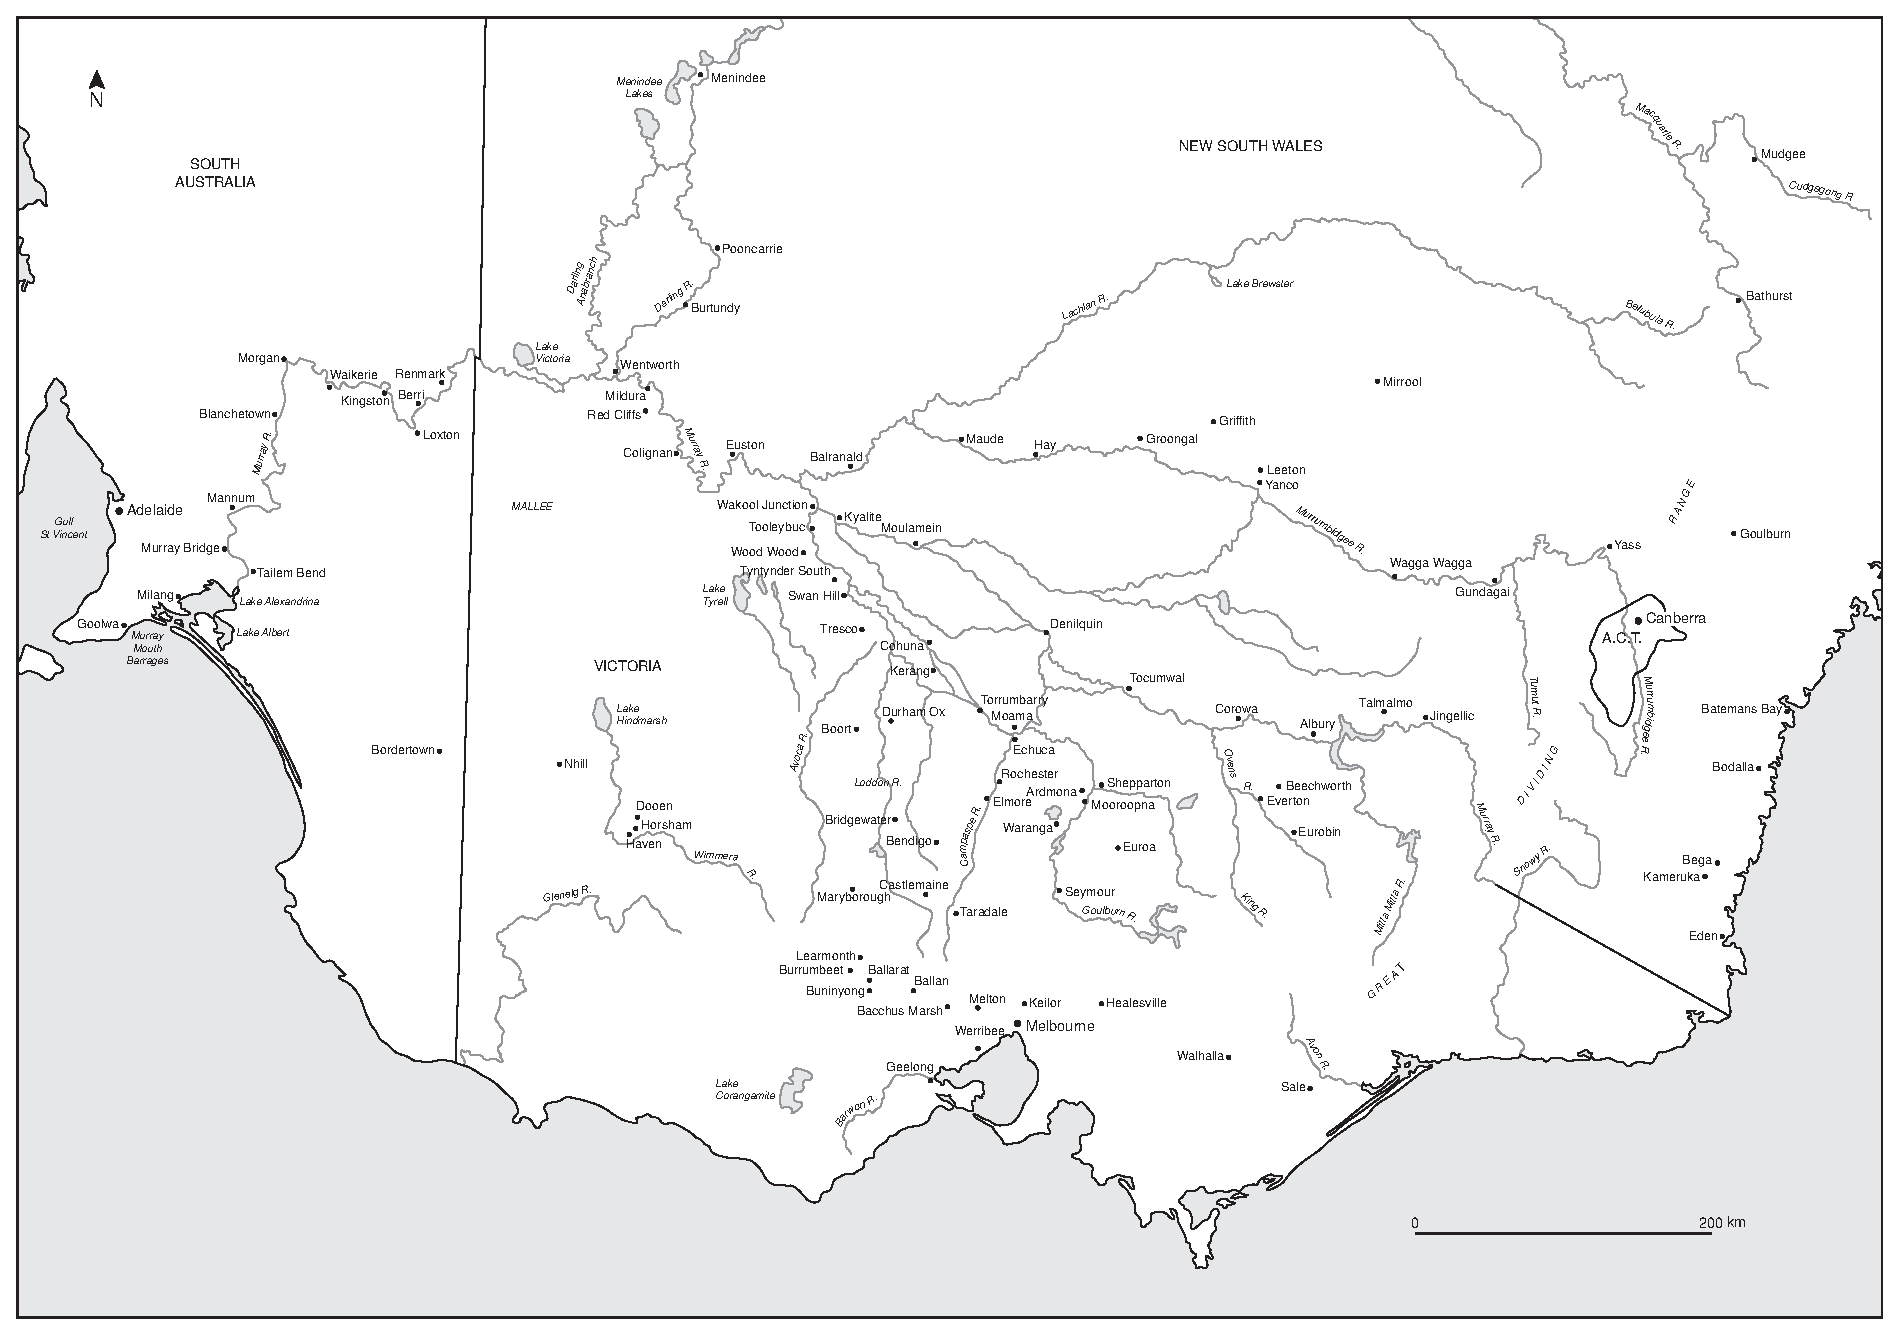
\includegraphics[bb=0 0 448 626,clip,width=1.123\textwidth]
{Figures/NSW_DOUBLE_PAGE.eps}}
\end{pspicture}
\newpage

\begin{pspicture}(0,0)(120mm,190mm)
\rput(48mm,96.2mm){
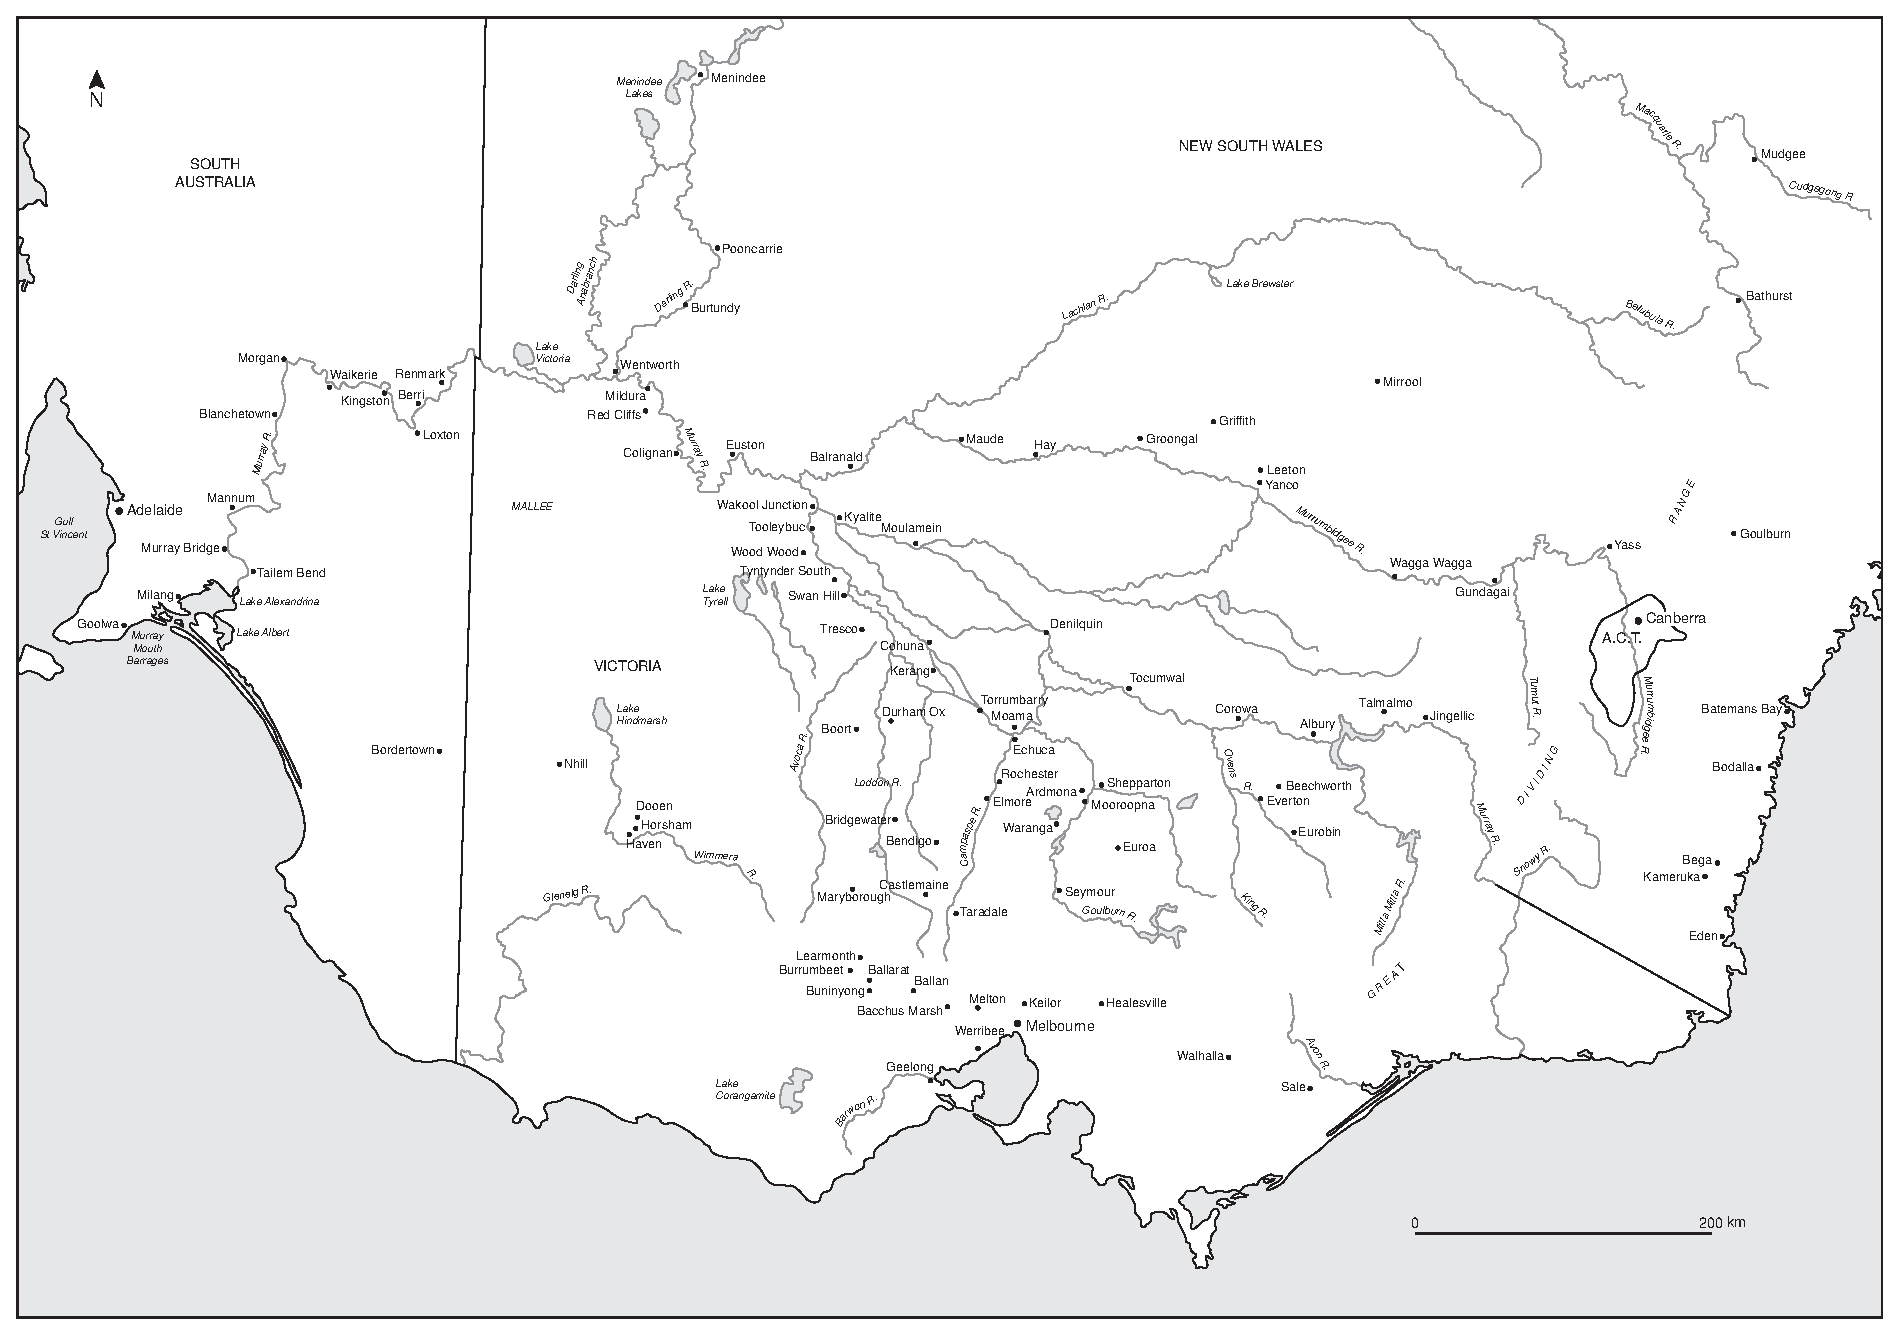
\includegraphics[bb=449 0 896 626,clip,width=1.123\textwidth]
{Figures/NSW_DOUBLE_PAGE.eps}}
\end{pspicture}
\vspace*{\fill}
\begin{center}
\sffamily
\textit{Rivers and sites of early irrigation in}\,
\textbf{South-Eastern Australia}
\end{center}
\newpage

\begin{pspicture}(0,0)(120mm,190mm)
\rput(55.5mm,96.2mm){
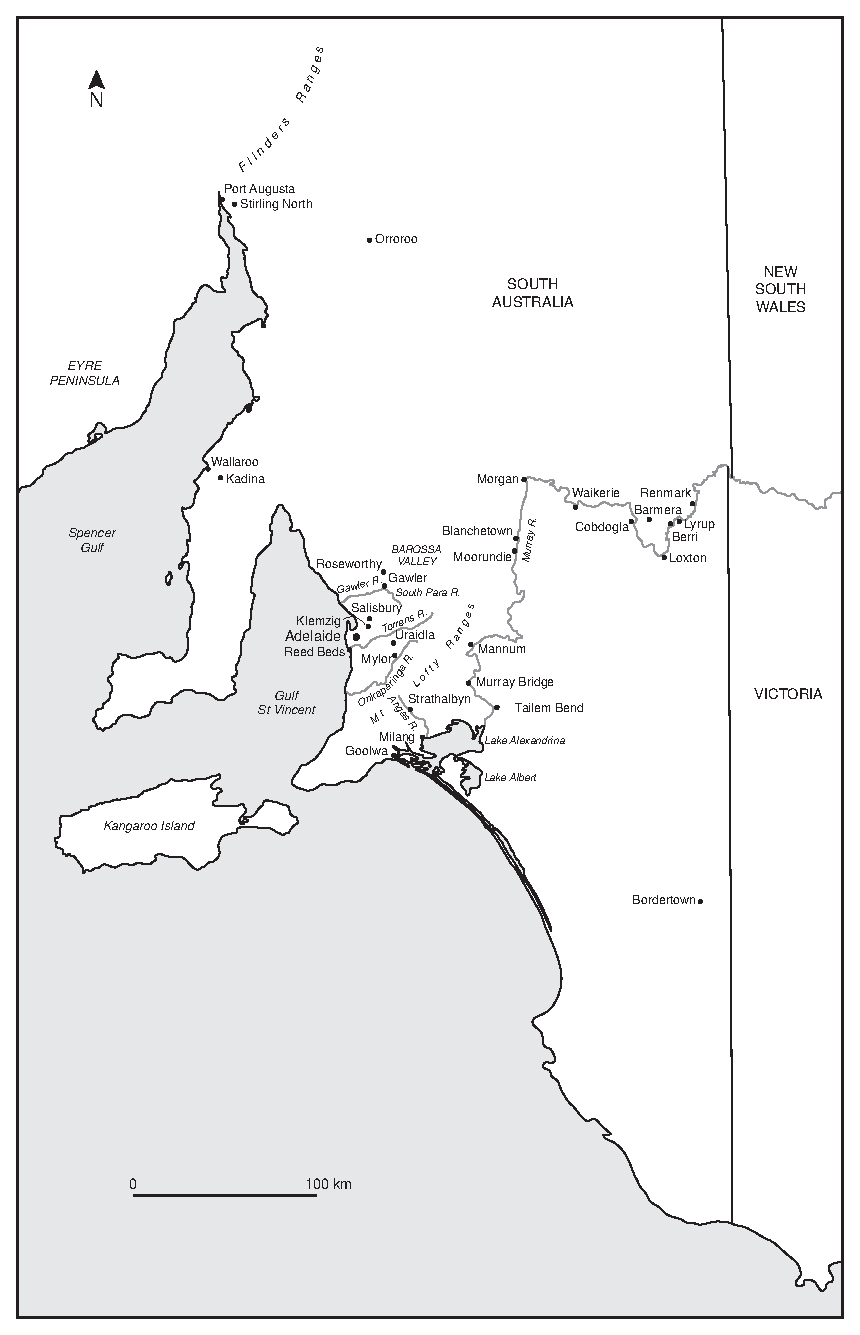
\includegraphics[width=\textwidth]{Figures/South_Australia.eps}}
\end{pspicture}
\vspace*{\fill}
\begin{center}
\sffamily
\textit{Rivers and sites of early irrigation in the} \textbf{Adelaide Region}
\end{center}
\newpage

\begin{pspicture}(0,0)(120mm,190mm)
\rput(55.5mm,96.2mm){
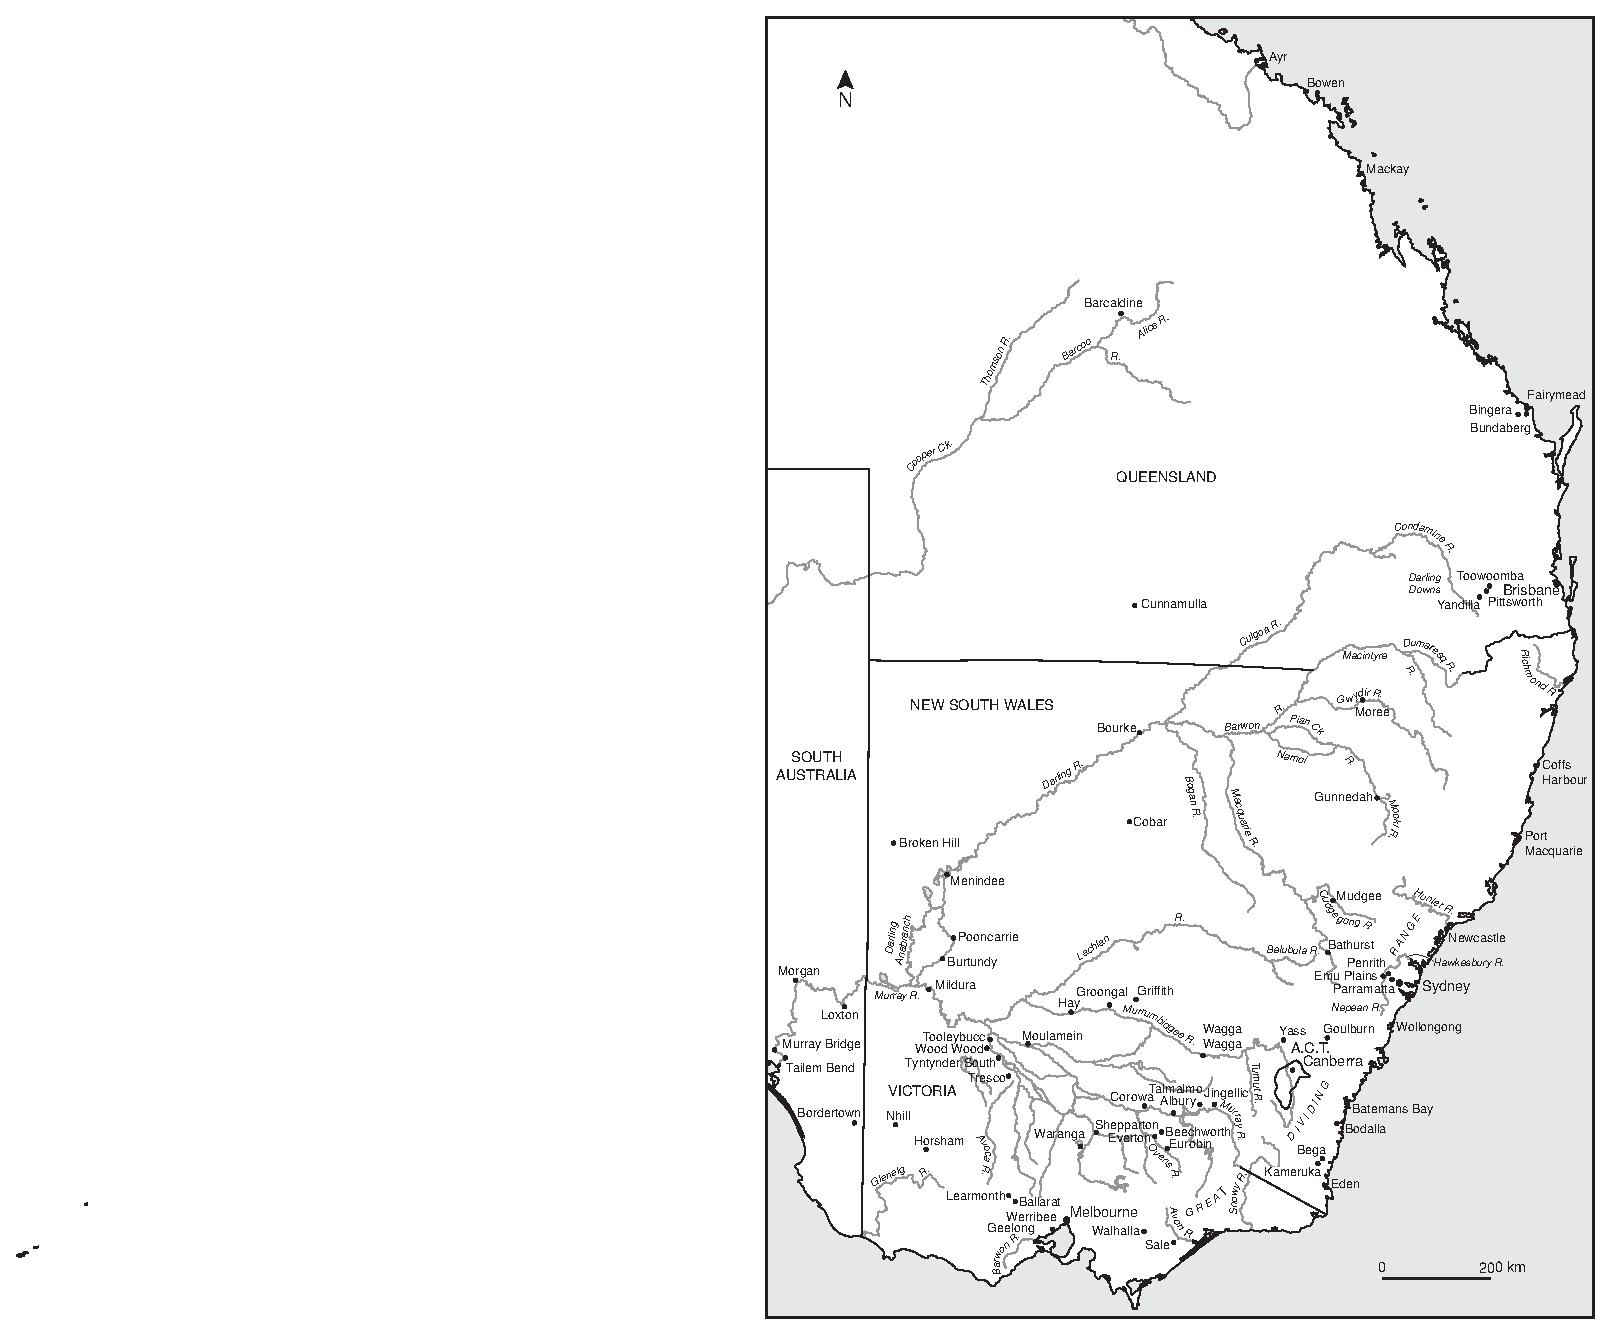
\includegraphics[width=\textwidth]{Figures/NSW_VIC.eps}}
\end{pspicture}
\vspace*{\fill}
\begin{center}
\sffamily
\textit{Rivers and sites of early irrigation in}\, \textbf{Eastern
Australia}
\end{center}
\newpage

\begin{pspicture}(0,0)(120mm,190mm)
\rput(55.5mm,96.2mm){
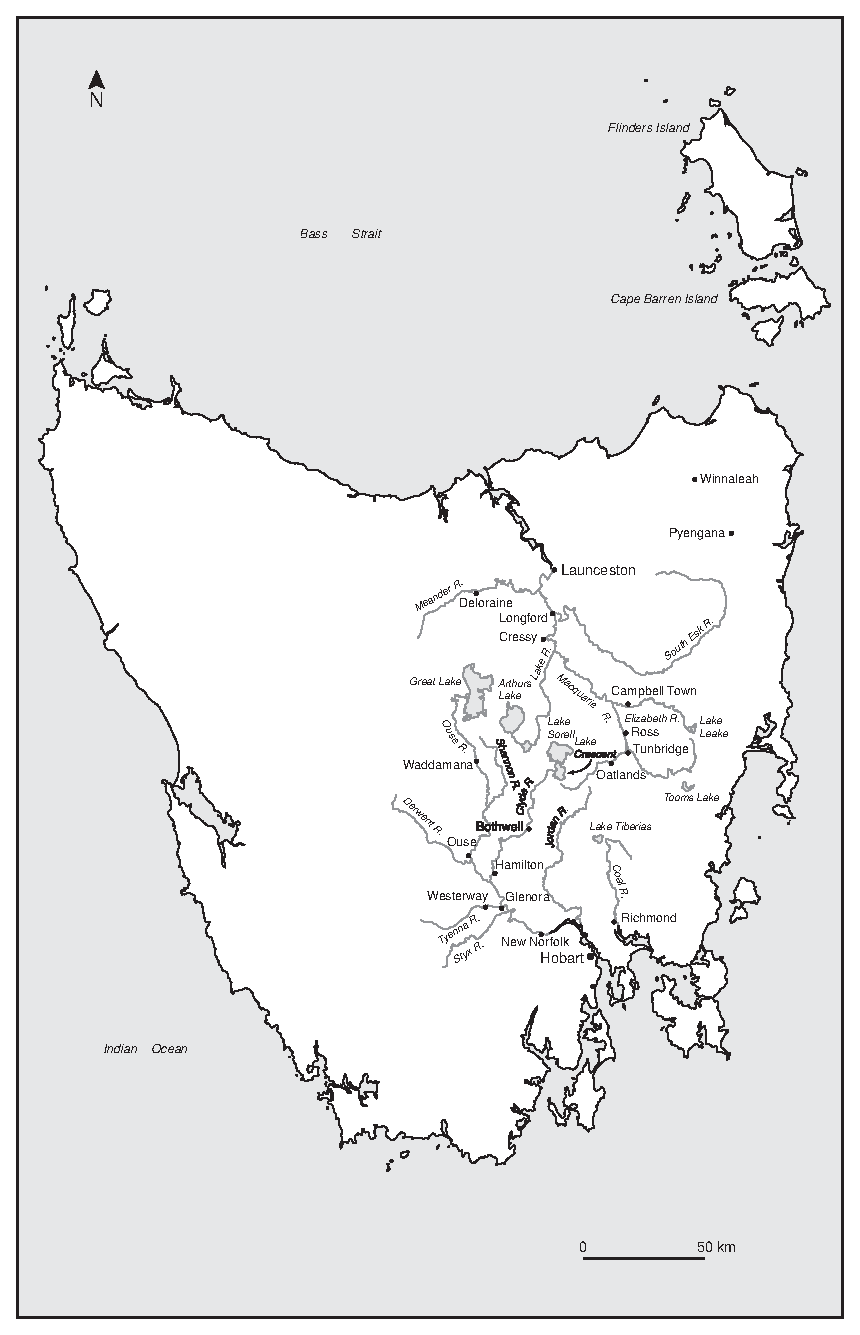
\includegraphics[width=\textwidth]{Figures/Tasmania.eps}}
\end{pspicture}
\vspace*{\fill}
\begin{center}
\sffamily
\textit{Rivers and sites of early irrigation in}\, \textbf{Tasmania}
\end{center}

% $Id$
% CHAPTER ONE
% 1389 words at 26/4/99

\setcounter{endnote}{0}

\chapter{Preface}
\label{ch:intro}
\addtoendnotes{\protect\subsection*{Preface}}

Irrigation was introduced to Australia by European settlers, probably
no earlier than the 1820s.  The Aboriginal people
constructed weirs and excavated channels but only to trap fish.
Accordingly there was no long-term experience of irrigation as in many
other parts of the world, but it has achieved great importance in
Australia, with impact in cities as well as the countryside.
Development at first depended on the skill and enterprise of
individual landholders, notably in Tasmania, who were able to draw on
nearby rivers.  Unsuccessful efforts were made in the 1840s and 1870s
to develop complex irrigation schemes and until the 1880s most
irrigation involved pumping rather than gravitation from perennial
streams.

When agricultural settlement extended on the mainland to inland tracts
with low unreliable rainfall the need for water soon led to interest
in irrigation and help was sought from colonial governments.  The
advice they first obtained from hydraulic engineers did not favour
irrigation but its progress in the United States encouraged popular
agitation in favour of government action at a time when the advantages
were being demonstrated in many parts of Australia by pastoralists,
farmers and Chinese market-gardeners.  At last steps
were taken in Victoria to establish irrigation through government
loans to locally based irrigation trusts and by agreement with two
Canadians who had developed irrigation settlements in California.
These projects were sustained for a time by the prosperity which then
prevailed in Victoria; they suffered during the subsequent depression
but provided valuable though costly experience.

A major outcome in the 20th century was to enshrine irrigation as a
matter primarily dependent on government intervention.  In
south-eastern Australia the governments of the three south-eastern
states on the mainland set up bodies with authority to establish
irrigation settlements catering for local residents and migrants, and
to regulate the use of water for irrigation.  In Tasmania, however,
different arrangements were made.

My interest developed through work as a soil scientist with the
Commonwealth Scientific and Industrial Research Organisation
(CSIRO). Its Division of Soils had been established in 1929, mainly in
response to problems of waterlogging and salinity affecting irrigated
lands in the Murray River valley.  It undertook classification and
mapping of soils, concentrating at first on the numerous irrigation
settlements and extending gradually to other areas.  When I joined
that Division in 1946 it was providing information on the soils of
areas intended for war service land settlement and one of my first
assignments was to take part in a survey of farm land at Loxton, South
Australia, before establishment there of an irrigated horticultural
settlement.  Related work was undertaken elsewhere by colleagues in
CSIRO and by others in state government bodies.  The publication of
soil maps and information on irrigation problems provided me with an
introduction to the complexity of irrigation in Australia.

Extending the domain of irrigation was widely accepted as progress
during the mid-20th century but the 1970s brought doubts, with the
focus on Murray Valley salinity problems and criticial studies of the
economics of irrigation.  These concerns influenced the changes in the
1980s affecting management of the River Murray and control of the
water industry in different States.  However, serious problems
continue to arise with irrigation.

During the 1970s I realised that the history of Australian irrigation
had attracted little attention and began its study.  The main
contributions then included the essay by Alfred Deakin, the biography
of George Chaffey, which provided information on the Chaffey
irrigation colonies of Mildura and Renmark on the River Murray, a
popular account of irrigation in the Murray valley and near the
Murrumbidgee River, and a chapter of a book mainly concerned with
economic aspects of Australian irrigation.\fn{\cite{deakin1892};
\cite{alexander1928}; \cite{hill1937}; \cite{davidson1969}.}

In the last quarter of the 20th century, the history of Australian
irrigation has been referred to in works dealing with institutions
responsible for water supply and irrigation, the celebration of the
Australian bicentenary, and the centenary of the Mildura and Renmark
settlements.  Only one of these publications is devoted entirely to
the development of irrigation in an Australian state: Tasmania. It was
followed recently by an account of the history of Australian
irrigation, which deals mainly with engineering aspects of events in
the twentieth century.\fn{\cite{masoncox1994}; \cite{hallows1996}.}

My aim has been for a comprehensive treatment of the pioneering period
of irrigation, showing the diffusion of experience among the colonies
or states, the contributions made by particular landholders,
engineers, and public figures, and the involvement of people from
various ethnic origins.  This book is concerned with developments up
to 1920 when the contemporary mix of government and private enterprise
was achieved.  While irrigation was always undertaken primarily for
better production by landholders in country districts, it had begun to
affect urban life through involvement with sewerage and by the
watering of parks, gardens and playing fields.

What is meant by irrigation?  Although definitions vary, they all
agree that the practice involves the application of water to the land.
Some assume that irrigation is concerned only with crop production,
but would exclude certain arrangements involving methods regarded as
primitive.  George Gordon, the hydraulic engineer with wide interest
in Victorian irrigation, advised that it is to be understood as:
%\begin{spacing}{1.0}
\begin{Quote}
	the conveyance of water without labour from a point where it
	is collected, or made available, to the lands to which it is
	to be applied, and its distribution over these lands. The term
	is also so used in connection with the utilisation of the
	sewage water of towns \ldots\fn{\cite{gordon1878}.}
\end{Quote}
%\end{spacing}
Another view is that irrigation includes `any process, other than
natural precipitation, which supplies water to crops'.  Irrigation
will be regarded in this account in the widest sense as the
application of water to land for a particular purpose.  Generally in
Australia it has been used in support of rural
industries.\fn{\cite{stern1979}.}

This book considers development of irrigation through three
significant periods.  The earliest runs from the establishment of
penal colonies to the impact of gold discoveries.  The unusual feature
of Australian irrigation is its lack of antiquity, and
chapter\,\ref{ch:early} concerns initiation of the practice.  The
remarkable early Tasmanian interest in its use and the relative lack
of it on the mainland are dealt with in chapters\,\ref{ch:tas}
and~\ref{ch:mainland}.  For the next period, distinguished by
Roberts\fn{\cite{roberts1924}.}  as marking the emergence of
agriculture, chapter\,\ref{ch:emergence} deals with irrigation in
south-eastern Australia by European farmers and Chinese
market-gardeners and with the campaign for an ambitious scheme for
provision of irrigation and transport by an extensive canal in
Victoria.

Irrigation in the last period, starting about 1875, became involved
with closer settlement in forms which included the gradual selection
of small holdings, the planned irrigation areas, and various
cooperative settlements.  Independent irrigators made an impressive
contribution, shown in chapter\,\ref{ch:indep}, the first for this
period, but they were gradually overshadowed by the involvement of
some colonial or state governments in irrigation following official
enquiries and legislation as outlined in chapter\,\ref{ch:inquiries}.
Then follow several chapters roughly in chronological order: four
dealing with irrigation used under different arrangements for closer
settlement (chapters\,\ref{ch:trusts}--\ref{ch:groups}), and others
concerning the association of irrigation with cities
(chapter\,\ref{ch:sewage}), the development of relations between
states concerning irrigation in the Murray--Darling drainage basin
(chapters\,\ref{ch:murray} and~\ref{ch:stateint}), and with the use of
underground water (chapter\,\ref{ch:underground}).

The fact that irrigation is a human accomplishment determined that my
account of its pioneering phase in Australia should give attention to
the interests and attitudes of the main players in the story together
with the engineering and agricultural aspects of the development.  My
study showed that progress in the pioneering phase of Australian
irrigation has involved serious controversy, occasional romanticism,
and technology transfer combined with local innovation; these
considerations should be reflected in the following account.


%\vspace{\fill}
%{\slshape
%\noindent
%Gerard (`Dick') Blackburn died on 6th August 1999, after completing
%the manuscript for this book.
%\begin{flushright}
%Hugh Blackburn\\
%Susan Blackburn\\[5pt]
%Melbourne, 2003
%\end{flushright}
%}
%%\section{References}
%%1. A.Deakin, Irrigation in Australia, in the Year-Book of Australia
%%   for 1892,pp 81-96.
%%2. J.A.Alexander, The Life of George Chaffey; A Story Of Irrigation
%%    Beginnings In California And Australia. 1928.
%%3. Ernestine Hill, Water Into Gold,1937.
%%4. B.R.Davidson, Australia Wet Or Dry?; The Physical And Economic
%%    Limits To The Expansion Of Irrigation, 1969.
%%5. Margaret Mason-Cox, Lifeblood Of A Colony; A History Of Irrigation
%%    In Tasmania, 1994.
%%6. P.J.Hallows \& D.G.Thompson, The History Of Irrigation In Australia,
%%   (1996?).
%%7.  G.Gordon, Lecture on Irrigation . . . and Drainage, 1878-79.
%%8. P.Stern, Small-scale Irrigation, 1979, as cited by A.Pacey,
%%    Technology In World Civilization, 1990.
%%9. S.H.Roberts,  History of Australian Land Settlement (1788-1920), 19 4.

\clearemptydoublepage
% $Id$

\chapter{Acknowledgments}
\label{ch:ack}

Considerable use was made of libraries and public records, including
the State Library of New South Wales (Mitchell Library and Archives
Authority), State Library of Victoria (La Trobe Library and Public
Rec\-ords Office), State Library of Tasmania, State Library of South
Australia (Mortlock Library and Bray Library, State Records Office of
South Australia, John Oxley Library, J.\,S.~Battye Library of Western
Australian history, Flinders University Library and libraries of the
University of Adelaide.

\medskip
Useful information or advice was given during a period of over
twen\-ty years by Ms~E.\,M.~Agar, Salomon Alba, Weston Bate, Susan
Blackburn, Hume Dow, G.\,P.\,H.~Dutton, R.\,W.~Gowlland, Mary Healy,
G.\,D. Hubble, C.~Mort, Esther Murray, Tom Patterson, Albert Rovira,
Lyndall Ryan, J.\,K.~Taylor, Elizabeth Whitcombe, L.\,W.~Weickhardt,
P.\,J.~Wischer, and by the Hawkesbury Historical Society, Mildura and
District Historical Society and the Shepparton and Goulburn Valley
Historical Society.

\medskip
Eunice Wilson undertook genealogical research in England and Anne Rand
supplied valuable information from Tasmanian archival material.

\clearemptydoublepage

%%%%%%%%%%%%%%%%%%%%%%%%%%%%%%%%%%%%%%%%%%%%%%%%%%%%%%%%%%%%%%%%%%%%%%%%%%%%%%
\mainmatter
\pagestyle{fancy}
\renewcommand{\headrulewidth}{0.4pt}
\fancyhead[LE,RO]{\sffamily \small \thepage}
\fancyhead[LO]{\sffamily \small Pioneering Irrigation in Australia}
\fancyfoot{}

% $Id$
% CHAPTER TWO
%3584 wds at 29/4/99

\setcounter{endnote}{0}

\chapter{The Earliest Irrigators}
\label{ch:early}
\addtoendnotes{\protect\section*{Chapter \thechapter}}
\markboth{\textsc{Chapter \thechapter. The Earliest Irrigators}}{}

Deliberate application of water from streams or springs to land in
Australia apparently began between 1820 and 1830.  There is no
indication that this practice followed direction from British
authorities, nor could it have been a response to the advice of
E.\,G.~Wakefield, the celebrated theorist of colonisation, whose
interest in Australian irrigation was expressed in 1829 and 1834.
Whether entirely fortuitous or owing something to contemporary usage
in Britain, its adoption certainly relied on the interest and
ingenuity of individuals far apart.  The first irrigation was
undertaken either in New South Wales or in Tasmania.  Elsewhere there
is evidence of irrigation before 1835 only from Western Australia
where settlement began in 1829.

\section*{New South Wales}
\label{sec:nsw}

It may appear curious that practical interest in irrigation in New
South Wales was not shown until at least thirty years after the
settlement at Port Jackson though probably much sooner in Tasmania.
The delay in starting the practice in New South Wales arose
principally from environmental constraints: climate and hydrology.

Governor Phillip's decision in 1788 to locate the penal settlement at
Sydney was more or less forced by his objections to Botany Bay and the
urgency of finding an alternative site to accommodate more than a
thousand people soon arriving in the First Fleet.  Though suitable for
mariners, Sydney Cove gave immediate access only to land which was
either too rocky or too sandy for successful food production, provided
only a small stream draining nearby swamps, and was encumbered by many
trees too hard for the axes brought from England.  A better site for
agriculture was soon found near the head of Port Jackson; the
settlement there came to be known as Parramatta and its growth for a
few years outstripped that of Sydney --- testifying to the
disadvantages of its site.  But the environs of Parramatta and its
residents, who generally had no previous agricultural experience,
failed to produce the amounts of food required; grain still had to be
imported.

Early exploration near Sydney had revealed the existence of a large
river draining from the distant hills known as the Blue Mountains and
discharging to the sea at Broken Bay, an inlet about 20 miles north of
Port Jackson.  This river, designated the Hawkesbury, was found to
traverse an extensive alluvial plain regarded as having great
potential for food production but too isolated at that stage from
Sydney or Parramatta.  Its occupation then by Aborigines was a further
initial deterrent to British intrusion.  Farming began there in 1794
after~22 settlers were each granted small holdings near the Hawkesbury
and a road was made from Sydney. Transport of goods to and from the
new settlement relied on the river until Governor Macquarie's order
for road improvement was achieved with completion in 1813 of the
turnpike road from Sydney to the river at Windsor.\fn{HRA I 1, 470,
483; \textsl{Sydney Gazette}, 27/11/1813, cited by
\citet[p.\,57]{bowd1982}.}

The Hawkesbury River generated many floods; there were ten between
1799 and 1819 which devastated crops nearby but despite this handicap
the district gradually came to be regarded as the granary of New South
Wales. Many settlers there had been convicts who qualified for small
grants of land after completion of their term of punishment. One was
Lawrence May who may have been the earliest irrigator in Australia. At
the age of eighteen he had been sentenced to death for breaking into a
shop in Dublin but the penalty was changed to transportation and he
arrived in Australia in 1791 aboard the Queen, known as a horror
ship. He began farming near the Hawkesbury after being granted a small
holding in 1800 and was successful enough to establish a horse-driven
flour mill in 1815; by 1828 he held 96\,ac at Pitt
Town.\fn{\citet[p.\,22]{johnson1991}; 
\citet[p.\,143]{bowd1982}.}

Floods on the Hawkesbury were a response to high rainfall in nearby
mountains, though the plain which the river traverses is by no means a
dry area.  The average annual rainfall at Sydney exceeds 47\,in, much
more than at any other early settlement on the Australian coast, while
at Windsor on the Hawkesbury the average is near 35\,in. The annual
rainfall is variable but its seasonal distribution is fairly uniform
except for a relatively dry spring.  Neither farmers nor pastoralists
had serious lack of water in most seasons and in the event of drought
there was generally scope for moving livestock to fresh grazing areas
on the Cumberland Plain between the mountains and the coast, or even
beyond the mountains to the Bathurst district following its discovery
after the drought of 1813.  There had been prolonged droughts in the
Sydney region frequently since 1788, but that commencing in 1826 was
the longest and most widespread yet known.\fn{J.\,B.~Henson, Eng.\
Assoc.\ NSW Proc.\ \textbf{6}, 1889; Comm.\ Bur.\ Meteorol.\ Bull.\
\textbf{48}, 1967.}

In describing this difficult period, the explorer Charles Sturt wrote:
\begin{quote}
	The year 1826 was remarkable for the commencement of one of
	those fearful droughts to which we have reason to believe the
	climate of New South Wales is periodically subject.  It
	continued during the following years with unabated severity.
	The surface of the earth became so parched that minor
	vegetation ceased upon it.  Culinary herbs were raised with
	difficulty, crops failed even in the most favourable
	situations.  Settlers drove their flocks and herds to distant
	tracts for pasture and water, neither remaining in the located
	districts.  The interior suffered equally with the
	coast.\fn{\citet{sturt1833}.}
\end{quote}

Conditions at Dunheved, about 12 miles south of Pitt Town on the
Hawkesbury, were described in some detail during the drought by
Harriet King in letters to her husband, Phillip Parker King, during
1827 and 1828. There was no complete lack of rain there but livestock
and crops suffered greatly until the spring of 1828 when falls of rain
ensured some return from the wheat crop.\fn{\citet{walsh1967}.}

It was during this serious drought that Lawrence May drew attention to
his efforts at irrigation.  The \textsl{Sydney Gazette} of
September~1, 1828, reported news it gathered a week previously:
\begin{quote}
	A Mr Lawrence May, a respectable settler at Pitt Town, has had
	the courage to erect a pump for the purpose of irrigating his
	land, an experiment, we believe, perfectly novel and
	unprecedented in the Colony. The pump is placed on the margin
	of the river, and conveys the water through lead pipes into a
	ditch, or trench, where it is conducted at pleasure, by means
	of furrows to any part of his farm. It is calculated that it
	will discharge 20 tons an hour, and requires only two men to
	work it. The first trial is to be made on Monday next, and a
	considerable number of respectable gentlemen intend to be
	present at so interesting a scene.
\end{quote}

Whether this trial was actually made is uncertain --- the Sydney
Gazette carried no news of it.  Lawrence May would have abandoned the
demonstration in the event of timely rainfall; it is possible that the
rain in the spring of that year, as mentioned by Harriet King, made
May's trial unnecessary.  There is another consideration which may
have deterred him.  Water then available for irrigation had become
brackish near Pitt Town and other farming settlements due to influx of
tidal water during the diminished flow of the Hawkesbury; normally the
river was fresh there and for 30~miles downstream.\fn{D.\,G.~Bowd,
personal communication.}  Whether the scheme reported in the press was
realistic for coping with a drought-stricken crop is uncertain: it
appears that arrangements for pumping would have provided water to a
depth of less than a quarter of an inch over 8\,ac after eight hours
of pumping.  Nevertheless nothing detracts from Lawrence May's
originality and ingenuity in his scheme for irrigation, apparently for
the first time in the colony.  His use of lead piping indicates a
capacity for procuring material then relatively scarce, though
probably used in construction of the first fountain erected in Sydney
at about that time.

Another indication of early interest in irrigation in the colony is
the report that James Macarthur, son of the pioneer wool-grower,
invented a scheme for mechanical irrigation in the late 1820s.  The
time of this development --- assuming it occurred in Australia ---
would have been before he travelled to England in 1828, where he
remained for a few years.  As with Lawrence May, experience of the
protracted drought of 1826--29 probably impelled Macarthur to devise
some means of watering plants of some value to him.  These were in the
gardens, orchards and vineyards at his
residence.\fn{\citet[p.\,492]{ellis1978}.}

During a further dry period during 1834--35 in the Sydney area, Sir
John Jamison took some interest in irrigation from the Nepean River,
which is continuous with the Hawkesbury, but it is uncertain whether
his plans came to fruition.  Jamison owned the imposing Regentville
mansion and land on the Nepean near Penrith; he was a wealthy man and
a leading member of the Agricultural and Horticultural Society of New
South Wales, founded in 1822.  Early in 1835 a Sydney newspaper
reported the importation of machinery for use in irrigation at
Regentville.  James Backhouse visited the property in October 1835,
noticed the effects of the prolonged dry season on the state of
Jamison's vineyard, but made no mention of irrigation undertaken by
the owner.\fn{\textsl{Sydney Monitor}, 3 Jan.\ 1835; 
\citet[p.\,338]{backhouse1843}.}

\section*{Tasmania}
\label{sec:tas}

In 1830 there was reference in the Hobart Town Almanack to irrigation
of a property near Hobart.  This may seem quite out of character with
the circumstances of land use on the island at the time; drought was
never the serious handicap it so often proved to be on the mainland.
Yet apparently irrigation was contemplated in Tasmania in little more
than twenty years after settlement at Hobart and it achieved some
popularity in the next two decades.  The developments depended on the
association of settlement with river valleys, experience gained
locally in the control of water resources, and the availability of
convict labour.

George Arthur arrived in Hobart in 1824 as the new
lieutenant-governor, shortly before Tasmania was made a colony
separate from New South Wales.  As a young army officer he had served
his regiment in different parts of the Mediterranean region.  Later he
was put in charge of the Colonial Office's interests in British
Honduras, where one of his activities during an eight-year term as
superintendent was to begin drainage of its swamps.  The latter
experience may have had significance for his private interest in
draining a swamp on the Derwent River near Bridgewater, upstream of
Hobart though still in its tidal reaches. The swamp covered
approximately 200\,ac of his farm which has been referred to as Dutch
or Marsh Farm.  An embankment was constructed with sluice gates to
allow drainage to the river at low tide, preparatory to the production
of meadow hay.  The sluice gates also may have been intended to allow
the entry of water for irrigation during periods of high river levels,
when the stream provided water of good quality.  The levels of the
river near the farm were subject to a tidal range of 3 to 4 feet at
the highest spring tide.\fn{\citet{shaw1967}; \citet{mckay1962}; 
J.~Moore-Robinson, The Haunted House, \textsl{Hobart Mercury}, 6 July
1935.}

Dr James Ross made reference to irrigation of this swamp in his
Almanack for 1830:
\begin{quote}
	A noble embankment has been completed, damming out the river
        effectually, which can, by sluices, be again let in so that
        about 200 acres may be most successfully irrigated in summer
        time, an advantage unequalled in the island, particularly in a
        dry summer. The quantity of rich meadow thus recovered from
        the river will always afford an adequate supply of
        hay.\fn{\textsl{Hobart Town Almanack} 1830, p.\,186.}
\end{quote}

Arthur's interest in this swamp started in 1826 when he began
acquiring properties which together made up Marsh Farm with an area of
almost 1400\,ac, including the swamp.  Productivity of the drained
swamp brought favourable comment from visitors; it became a show place
during the 1830s as indicated in 1833 by Mrs~Princeps.  Almost
directly across the river, a similar formation was reclaimed by Arthur
Davies and managed by the distinguished convict Henry Savery; its
embankment also involved sluice gates but no indication of their use
for irrigation is given in a comprehensive account of both swamps.
The main problem in using these areas was apparently drainage: wide
internal drains were needed as well as maintenance of the sluice
gates.\fn{\citet{gowlland1980}.}

When George Arthur left Tasmania in 1836 his properties were
administered by his former secretary, William Thomas Parramore, who in
March 1849 wrote to Arthur about drainage of the swamp.  His letter
tells of advice given by James Blackburn, the engineer then engaged on
bridge construction nearby at Bridgewater, and by Roderic O'Connor,
well known for his practical knowledge of farming in Tasmania.  The
engineer proposed the installation of pumps to improve the swamp and
in view of the probable expense Parramore consulted O'Connor.  The
latter advised Parramore that:
\begin{quote}
	\ldots he had a strong Lincolnshire navigator who understood
	drainage and banking by practice and that if it was possible
	to recover the Marsh this man would do it. \ldots His opinion
	I regret to say is far from encouraging.  The Fens, he says,
	in Lincolnshire that have been reclaimed rest on a substratum
	of clay four or five feet beneath the surface, upon this the
	banks are made and they are puddled with the clay.  Now at the
	Marsh there is peat to the depth of ten feet at least, a pole
	can be thrust down to that depth and no solid bottom is
	reached.\fn{Sir George Arthur papers, ML Ref.\ FM4/2688,
	Letter 13 March 1849, from W.~Parramore to Sir George Arthur.}
\end{quote}
This information suggests that the swamp could not be drained
successfully because of the depth of peat, so a need for irrigation
was unlikely to arise.  This farm was sold in 1854.

Another use of irrigation, associated with water-powered mills, may
have preceded the drainage of Governor Arthur's farm.  In one case,
relating to the property on the Derwent River once known as
Humphreyville but later as Bushy Park, `extensive irrigation works
with a flour mill' were reported as installed about 1820 by the owner,
Adolarius William Henry Humphrey, an important public servant.
Humphrey's farm was visited in December 1826 by the land commissioner
Roderic O'Connor, who found it presented `one of the most gratifying
sights in the colony', commented on the crops and livestock but failed
to mention any use of irrigation.  However, there were facilities for
diversion of water from an adjoining stream when the property was
bought by Ebenezer Shoobridge in 1864.\fn{\citet{stancombe1968};
\citet[pp.\,56--58]{masoncox1994}; \citet{mckay1962}.}

Irrigation in the Midlands as early as 1825 has been suggested by
reference to diaries kept by James Cubbiston Sutherland. He has been
credited with construction in March 1825 of an `irrigation channel
from a brook to his farm'. However, Sutherland's diary for~1 and~2
March 1825 shows that one of his assigned servants and another man
worked with Andrew Gatenby `in cutting a course for the water through
the lagoon'.  Gatenby and Sutherland had travelled together to
Tasmania in 1823 and soon obtained grants of land on the Isis River
near its confluence with the Macquarie, Gatenby's Barton homestead
being two miles from Sutherland's Rothbury.  Later in March, when
water was flowing after rain, Sutherland's men spent three days with
Gatenby `securing the embankment for his mill dam', and Gatenby's mill
was recorded as `at work' before April.  These entries indicate that
Sutherland had no direct involvement in cutting a channel but was
providing help to a neighbour and friend who sought adequate water for
his mill.\fn{\citet[p.\,138]{morgan1992}; J.\,C. Sutherland Diaries,
TA, \textbf{1}; \citet[p.\,64]{brown1941};
\citet[pp.\,22--23]{mckay1962}.}

In 1829 there were 29 flour mills operating on the island, with all
but four driven by water.  Practically all had been installed since
1818.  Whether the water leaving such mills was returned to its
natural course or allowed to spread over the ground was possibly not a
matter deserving comment although irrigation may have been
involved. However, by the late 1830s at least one instance of the
association of water-mills with irrigation had become known to a
Tasmanian writer, David Burn.\fn{\citet[p.\,129]{linge1979}; 
\citet[p.\,96]{burn1840}.}

\section*{Western Australia}

British settlement on the Swan River began in 1829 and irrigation was
undertaken by 1834.  The town of Perth was established in 1830 on the
banks of the Swan River in its tidal reach but fresh water was
available from local swamps and springs.  Captain Frederick Irwin, in
charge of the military detachment to protect the new settlement,
reported the use of irrigation before 1835 on his property in the Swan
River valley.  He came to Western Australia in June 1829, remained
there more than four years, and returned in 1837 for seventeen years.
Irwin soon had a house on land acquired in Perth and later added to
his property by acquisitions further inland.  Together with his
cousin, William Mackie, the advocate-general, he took up 3240\,ac in
the Swan River valley in 1829--30 and 7000\,ac near York on the Avon
River.  Their farm known as Henley Park was on the Helena River,
tributary to the Swan.  It was one of several properties in the
district that were acquired by members of the new colonial
administration.  A prime attraction there was the extent of alluvial
soils superior in quality to the sandy types so prevalent on the Perth
coastal plain.  However, it shared the general lack of adequate rain
in summer.  The locality had the advantages of being just beyond the
tidal influence on the river and accessible by boat from Fremantle and
Perth.  Guildford, 7~miles northeast of Perth, became its main
township.\fn{\citet{mossenson1967}; \citet{honniball1967};
\citet[appendix]{ogle1839}.}

Irwin and Mackie were extremely fortunate in having Richard Edwards as
manager of their rural properties.  He was one of the hundreds brought
out in 1830 by Thomas Peel, whose late arrival led to a debacle for
his grandiose scheme to settle up to a million\,ac south of the Swan
River.  His chosen area had then been allotted to others and Peel was
offered inferior land further south; various upsets to his plans made
the hundreds of prospective settlers discontented and his scheme
failed by 1833.  Edwards had skills in brick and tile-making as well
as in farming, gardening, brick-laying, lime-burning, and brewing.
One of his sons was a carpenter; another was a ploughman.  It was
Edwards who carried out irrigation at Henley Park.

Irwin gave handsome testimony to Edwards and his work in his book
written early in 1835 in England.
\begin{quote}
	In the improvement of the gardens he takes peculiar delight,
	and is very successful, having a good knowledge of
	horticulture, acquired by serving an apprenticeship to a
	market gardener.  The spot he fixed upon for his first one was
	a somewhat elevated morass, on sloping ground, separated from
	the house by a ravine, and covered with rank vegetation owing
	to latent springs.  These, after burning off the surface, he
	dug out, and formed into circular wells of close and
	substantial brickwork, rising several layers above the
	surface; from these wells, at different elevations, he is
	enabled to conduct the water in channels to almost every part
	of the garden.  When the last accounts left, he was
	constructing earthen pipes for the purpose of completing his
	plans of irrigation, and also for conveying water across the
	ravine to the height on which the house is situated.  In this
	garden, and in another larger one, hereafter to be noticed,
	almost every kind of vegetable, and as many sorts of
	fruit-trees as have been introduced from tropical and
	extra-tropical countries, are found to flourish.  Among the
	former was the mangel-wurzel, already mentioned as having a
	root six feet in circumference, the tomato grows luxuriantly,
	weighed down with the load of its beautiful
	fruit.\fn{\citet[pp.\,57--60]{irwin1835}.}
\end{quote}

\section*{Conclusion}
\label{sec:conc}

The several references to early irrigation include those with some
telling details concerning use of water in aid of plant growth and
others giving only the bare mention of irrigation. These latter
references are unsatisfactory since in one case the term irrigation
related to channeling to convey water to a mill.  The most compelling
evidence for early irrigation clearly relates to Lawrence May in 1828,
but so far there is nothing to show that his plans for irrigation were
actually carried out.\fn{\citet{morgan1992}.}

%\section*{References}
%1. HRA I 1, 470,483.
%2. Sydney Gazette,27/11/1813, cited by D.G. Bowd, Macquarie Country
%   1982, p.57.
%3. K.Johnson \& M.Flynn, Convicts Of The Queen, p.22, in Exiles From
%     Erin (ed R.Reece), 1991.
%4. Bowd 1982, p.134, \& K.Johnson \& M.Flynn, Convicts Of The Queen, 1991.
%5. J.B.Henson, Eng.Assoc.NSW Proc. vol.6, 1889.
%6. Comm.Bur.Meteorol.Bull. 48, 1967.
%7. C.Sturt, Two Expeditions Into The Interior Of Southern
%   Australia,1833,vol.1,p.1.
%8. Dorothy Walsh(ed), The Admiral's Wife. Mrs Phillip Parker King, A
%    Selection Of Letters 1817-56, 1967.
%9. Sydney Gazette, 1/9/1828.
%10. Pers. comm. D.G.Bowd.
%11. M.H.Ellis, John Macarthur, 1978, p.492.
%12. Sydney Monitor, 3/1/1835.
%13. J.Backhouse, A Narrative Of A Visit To The Australian Colonies,
%    1843, p.338.
%14. A.G.L.Shaw, Sir George Arthur, ADB vol.1,p.32.
%15. J.Moore-Robinson, The Haunted House, Hobart Mercury, 6/7/1935.
%16. Anne McKay(ed), Journals Of The Land Commissioners For Van
%      Diemen's Land, 1826-28, Hobart, 1962, p.114.
%17. Hobart Town Almanack 1830, p.186.
%18. R.W.Gowlland, Some Van Diemens Land Affairs, 1980, p.118.
%19. R.W.Gowlland, 1980.
%20. Sir George Arthur papers, ML Ref. FM4/2688, Letter 13 March
%      1849,from W.Parramore to Sir George Arthur.
%21. G.H.Stancombe, ADB vol.1,1968, p.565, \& Margaret Mason-Cox,
%      Lifeblood Of A Colony, A History Of Irrigation In Tasmania,
%      1994, pp56-58.
%22. Anne McKay(ed), 1962.
%23. Margaret Mason-Cox, 1994 pp.56-58.
%24. Sharon Morgan, Land Settlement In Early Tasmania, 1992, p.138.
%25. P.L.Brown(ed). Clyde Company Papers, vol.1, 1941 p.64.
%26. J.C.Sutherland Diaries, TA, Vol.1, \& Anne McKay(ed),1962  pp22-23.
%27. G.J.R.Linge, Industrial Awakening, 1979, p.129.			
%28. David Burn, A Picture Of Van Diemens Land, 1840/1973,p.96.
%29. D.Mossenson, F.C.Irwin, ADB vol.2, 1967, p.5.
%30. J.H.M.Honniball, W.H.Mackie, ADB vol.2,p.174, \& N.Ogle, The Colony
%      of Western Australia, 1839/1977, Appendix.
%31. F.C.Irwin, The State And Position Of Western Australia, 1835, pp57-60.
%32. Sharon Morgan, 1992.

\clearemptydoublepage
% $Id$
% CHAPTER THREE
% at 29/4/99 4898 wds

\setcounter{endnote}{0}
\chapter{Tasmania 1835--1855}\index{Tasmania}
\label{ch:tas}\addtoendnotes{\protect\subsection*{Chapter \thechapter}}
\markboth{Chapter \thechapter. Tasmania}%
{Pioneering Irrigation in Australia}

Although irrigation apparently failed to take hold in Tasmania in the
1820s, it certainly flourished in the late 1830s to a much greater
extent than in any mainland colony.  This development on land rarely
troubled by serious drought may seem remarkable.  Once adopted, the
practice continued in several parts of Tasmania for many years.
Individual landholders displayed initiative, technical advice was
available, and the authorities took some action to develop this
facility.

Although dominated by use as a penal settlement, Tasmania attracted
many settlers, able until 1834 to secure free grants of land, to an
environment somewhat comparable to parts of the British isles.
Attractive valleys with rivers fed from lakes and mountains, a mild
climate, and low frequency of widespread droughts appealed to British
adventurers, farmers, and retired army officers.  A further appeal for
prospective settlers was the availability of convict
labour. \index{convict labour} Under the assignment system then in
force, a landholder was allotted a number of servants in proportion to
the size of his property on condition that he clothed, supported and
accommodated them at his own expense.  This supply of labour was
additional to other servants brought from Britain or India. The
settlement in Tasmania had a dual-purpose nature: `both a free colony
and a gaol'.\fn{\citet[p.\,97]{roberts1924}; K. Fitzpatrick~(1967),
ADB
\textbf{1}, p.\,413.}

Contemporary accounts point to use of irrigation between 1835 and 1840
but the identity of some operators is unknown and details of its
application are generally unavailable.  James
Backhouse,\index{Backhouse, J.} the Quaker missionary who travelled
widely in Australia and recorded much of its natural and social
features, lived in Tasmania during 1832--34 and made a return visit in
February 1836 when he first learnt of irrigation recently undertaken
near the town of New Norfolk on the Derwent
River.\index{river!Derwent} David Burn's\index{Burn, D.} well-informed
articles
\citep{burn1840} were published in London, with the claim that
irrigation in Tasmania was `a practice that has recently become one of
general adoption.'  Arthur Cotton,\index{Cotton, A.} an engineer who
took a special interest in Tasmanian irrigation from 1839 to 1843,
wrote in 1840 that several landowners in different parts of the island
had increased production by irrigation which was used on improved and
natural pasture and in wheat-growing.  He also wrote under a pseudonym
in 1849 that for the previous fifteen years in Tasmania,
lucerne\index{lucerne} under irrigation had provided a cutting `about
fifteen inches high every three weeks, throughout the spring and
summer'.\fn{\citet[p.\,348]{backhouse1843}; \citet{cotton1842};
\citet{cotton1849}.  `Delta' was identified as Authur Cotton by G.~Gordon
\citeyearpar{gordon1900}.}

\section*{The Irrigators}

One of the earliest irrigators was Alexander Reid\index{Reid, A.}
(1783--1858), who came to the island in 1822 and obtained grants of
land on the River Clyde,\index{river!Clyde} a tributary of the
Derwent. On this property of 1400\,acres known as Ratho,\index{Ratho
estate} Reid gained success as a wool producer.  Ratho was advertised
for sale in 1837 with advice that the English grass paddocks were then
under irrigation from the Clyde.\fn{\textsl{Hobart Town Courier}, 20
Oct.\ 1837, as cited by
\citet[p.\,17]{masoncox1994}.}

Michael Fenton\index{Fenton, M.} (1789--1874) was probably the first
to combine irrigation with the use of a water-mill.
\index{water-mill} He came to the
island in 1828 after twenty years with the British army in India and
obtained a grant of 1970\,acres on a tributary of the Derwent River
near New Norfolk.\index{New Norfolk, Tas.} In 1829 he went to live on
the property, later identified as Fenton Forest, where a few years
later a group of 76 men, women, and children arrived as his indentured
servants.  David Burn mentioned his use of irrigation, apparently
before 1840:
\begin{quote}
	Taking advantage of the latter river (Russell Falls), \ldots
	Captain Fenton \ldots has formed a watercourse whereby he
	drives a threshing machine and flour mill, supplies his house,
	and then irrigates an extended flat of the richest
	soil.\fn{\citet{robson1967}; \citet[p.\,96]{burn1840}}
\end{quote}

Another early irrigator may have been Francis Bryant,\index{Bryant,
F.} who leased Redlands\index{Redlands, Tas.} comprising 1550\,acres
on the Derwent River near New Norfolk.  The \textsl{Austral-Asiatic
Review} claimed in 1843 that Bryant was the first settler in the
colony to practice irrigation.\fn{\citet[p.\,6]{masoncox1994}.}

From 1840 there was greater interest.  One of the first to become
involved then was William Kermode.\index{Kermode, W.}  In that year he
tried irrigation on his Mona Vale\index{Mona Vale, Tas.} estate in the
Midlands, using water from a tributary of the Macquarie
River.\index{river!Macquarie} Neighbours who soon followed suit
included Thomas Parramore\index{Parramore, T.} of
Wetmore\index{Wetmore, Tas.} (3062\,acres), Samuel
Horton\index{Horton, S.}  of Somercotes (1045\,acres) and Phillip
Smith\index{Smith, P.} of Syndal.  At about the same time irrigation
was begun at Lawrenny, a large estate lying between the Clyde
\index{river!Clyde} and Ouse Rivers\index{river!Ouse} and owned by
Edward Lord,\index{Lord, E.} one of the richest men in the colony.
Kingston,\index{Kingston, Tas.} a property 12 miles south-east of
Launceston\index{Launceston, Tas.} was advertised for sale by Edmund
Bryant in 1841 as having 200\,acres sown down to English grass and
clover, all under irrigation from the Ben Lomond
Rivulet.\index{river!Ben Lomond} Hunterston, a property of more than
4000\,acres held by the family of Myles Patterson\index{Patterson, M.}
on the Shannon River\index{river!Shannon}\,---\,part of the Derwent
river system\,---\,was irrigated from January 1842.  David
Jamieson\index{Jamieson, D.}  irrigated wheat before 1843 on his
property, Glen Leith, near New Norfolk.  The property of 1800\,acres
known as Blair on the Clyde River was advertised for sale in 1843 on
the death of its owner, William Allardyce,\index{Allardyce, W.} with
information that 60\,acres of English grasses were under
irrigation.\fn{\citet[p.\,40]{masoncox1994}, `Bruni', Irrigation in
Tasmania; \textsl{Australasian}, 3 Nov.\ 1883;
\textsl{Hobart Town Courier}, 12 Nov.\ 1841; K.\,R.~von~Steiglitz, The
History Of Bothwell, 1958, cited by \citet[p.\,26]{masoncox1994};
\citet[p.\,417]{strzelecki1845}; \citet[p.\,20]{masoncox1994}.}

The popularity of irrigation in Tasmania in the early 1840s is
suggested by advertisements of properties for sale.  Prospective
buyers of the Rosenvale estate of Anthony Williams\index{Williams, A.}
on the Back River,\index{river!Back} New Norfolk, were advised that
its area of 160\,acres included a dam and sluice gate with troughing
erected for irrigating the meadow land, through which the Back River
flowed with a sufficiency of water at all times to turn a mill.  The
Ashby estate of 2800\,acres on the Macquarie
River\index{river!Macquarie} was advertised with the claim that
following the successful outcome of water conservation at Tooms
Lake,\index{lake!Tooms} `a very large proportion of the property
\ldots may be subjected to irrigation.'  Several notices in March and
April 1842 concerning properties to let or for sale in northern
Tasmania made reference to possibilities for irrigation: several farms
to let in the Deloraine\index{Deloraine district, Tas.} district,
about 25\,miles west of Launceston, were claimed as `being capable of
irrigation'; another four properties were similarly mentioned
later.\fn{\textsl{Hobart Town Courier}, 8 Mar.\ 1840;
\textsl{Launceston Advertiser}, 18 Feb.\ 1841; \textsl{Cornwall
Chronicle}, 5 Mar.\ 1842, 9 Apr.\ 1842.}

Even more telling of the vogue for irrigation was the publication of a
news item under the heading `Want of Water' which reported the plight
of those whose mills were `unable to work at present for the want of
water; the cause of which is ascribed to be the mania for
irrigation'.\fn{\textsl{Cornwall Chronicle}, 9 Apr.\ 1842.}  This may
be the earliest indication that irrigation in Tasmania might lead to
disputes over the riparian rights of landholders with river frontages.
However, irrigation in the early 1840s does not appear to have
involved a very large area: half of the dozen or so properties then
involved no more than 2500\,acres under irrigation.

In the period 1845--50 there were apparently few additions to the
irrigated properties.  Part of an area of 6000\,acres near Deloraine
in northern Tasmania, granted to Thomas Archer\index{Archer, T.} in
the 1820s; was irrigated from the Meander River\index{river!Meander}
by 1848, when his son William Archer\index{Archer, W.} went to live
there, designed the house named Ches\-hunt, and later used his
engineering skill to develop irrigation on the property.  Isaac
Sherwin,\index{Sherwin, I.} a Launceston merchant, retired in 1845 to
Sherwood, his father's property near the Clyde.  He began irrigation
there about 1847 and later extended its use after constructing a
tunnel to provide more water.  It is probable that irrigation at
Dennistoun,\index{Denniston, Tas.} also near the Clyde River,
\index{river!Clyde} was begun in
this period.  Irrigation for hop-growing\index{hops} may have been
started by Ebenezer Shoobridge\index{Shoobridge, E.} about 1849 at
Glen Ayr, near Richmond.\fn{\citet[pp.\,28, 24, 50]{masoncox1994};
Tasm.\ J.\,Agric.~\& Hortic.\ August 1860}

During 1850--55 irrigation failed to attract more landholders, though
there is evidence of additional areas provided by William Archer at
Saundridge near Cressy.\index{Cressy,
Tas.}\fn{\citet[p.\,30]{masoncox1994}.}

\section*{Motivation}

Tasmanian irrigation developed in response to favourable opportunities
for exports.  Sales of wool\index{wool} to Britain became significant
by the mid 1820s and in 1830 the island supplied more wool than the
mainland.  Rapid extension of sheep-grazing in south-eastern Australia
during the 1830s involved many Tasmanians who crossed Bass Strait to
become squatters on new sheep runs south of the River
Murray\index{river!Murray} or made settlements soon designated as
Melbourne\index{Melbourne, Vic.} and Geelong\index{Geelong, Vic.} on
Port Phillip Bay.\index{Port Phillip Bay} The initial success of
pastoralists in this part of the mainland created a demand for sheep
to stock the extensive natural pastures, both in the Port Phillip
District and, after 1836, in the new colony of South
Australia.\index{South Australia} The new settlements also required
foodstuffs and for a period Tasmania became the granary for people
everywhere on the mainland and was also an important source of
potatoes.  The area under wheat in Tasmania rose from 31\,156\,acres
in 1830 to 60\,813\,acres in 1840.  These favourable conditions for
landholders during the 1830s enabled some to build mansions, or to
make farm improvements including irrigation which would both increase
production and enhance the market value of properties.  A vast amount
of agricultural and construction work before the early 1840s was done
by assigned convicts.\fn{\citet[p.\,207]{fitzpatrick1941};
\citet[p.\,133]{hartwell1954};
\citet[p.\,445]{coghlan1918}.}

The principal use of irrigation in this period was to improve fodder
production in summer and autumn for sheep and cattle. Summer grazing
was available on river flats, parts of which were swamps of no value
in wetter seasons.  Irrigation of these lowlands in drier seasons gave
better production of fodder; it generally relied on gravitation of
stream water diverted by a weir upstream.  This arrangement, most
appropriate for a property large enough to embrace the stream frontage
suitable for a gravitational system, was also generally required for
water-mills, so an association of milling and irrigation developed in
some places and proved advantageous in summer and autumn.  Utilisation
of low-lying areas by drainage combined with their irrigation in drier
seasons was apparently intended before 1830 for Governor Arthur's
Marsh Farm; it was certainly achieved by William Kermode on his
property in the Midlands.  Irrigation was used for some crops of
wheat, though rainfall in winter and spring was generally sufficient
to produce good crops.

\section*{Technology Transfer}

The early irrigation in Tasmania may be related to
British\index{Britain} experience following invention of artificial
flooding or `floating meadows' by Rowland Vaughan\index{Vaughan, R.}
in Herefordshire during the 16th century.  By the 1850s irrigated
meadows in eleven English counties accounted for more than 8~per cent
of their total area under grass, so the practice may have been known
to Tasmanian landholders trying to follow the best British farming
methods.  `Floating the meadows' has been compared with the `marcite'
system of irrigation used in northern Italy,\index{Italy} where
relatively warm river water is applied to meadows in winter and early
spring with the aim of displacing the colder stagnant water in the
soil and stimulating early production of fodder.  This winter
irrigation is referred to in English references as floating the
meadows, but the title of Robert Vaughan's book (1610) shows a wider
interpretation: `The Most Approved and Long Experienced Water Workes.
Containing the Manner of Winter and Summer Drowning of Meadow and
Pastures.'\fn{\citet[pp.\,110--5]{kerridge1973};
\citet[p.\,1042]{mingay1989}.}

Adoption of irrigation on the island may have been influenced also by
the arrival of British people aware of its value from residence in
India.  The attractions of Tasmania for these people probably became
known through movement of British regiments between India\index{India}
and Australia, The most obvious early example of reference to Indian
experience is given by the activities of Arthur Cotton\index{Cotton,
A.} in Tasmania.  After service with the East India Company's military
forces as an irrigation engineer in southern India, he arrived late in
1838 on the first of two long periods of sick leave.  He visited
different parts of the settled districts during 1839 and 1840,
witnessed the existing use of irrigation, and personally advised
landholders on the technical measures
involved.\fn{\citet{blackburn1985}.}

Arthur Cotton had been involved with the maintenance of
long-est\-ab\-li\-shed irrigation systems dependent on monsoon rains.
He had experience of diverting water from a large river to supply an
extensive irrigation system at Tanjore, and he was familiar with the
widespread use of reservoirs (tanks) to conserve water for crop
production in the dry season.  In Tasmania he was thus able to advise
on dams, water conservation, and irrigation systems.  The full extent
of his assistance to individual landholders is unknown but many
details of his activity in the Macquarie River\index{river!Macquarie}
valley have been recorded.  Before returning to duty in India in 1840,
Cotton set out his views on irrigation in Tasmania in a paper
published later by the Tasmanian Society.  His statement notes the
opportunities for irrigation in a land where streams generally had
either a lake or lagoon at their headwaters, thus providing
opportunities for storage by construction of embankments or dams.  He
also gave estimates of evaporation, detailed advice on construction of
dams and races, and discussed various mechanical ways of raising water
from streams.\fn{\citet{cotton1842}.}

Finding that much Tasmanian land was capable of improvement and that
agricultural production would remain the main source of wealth on the
island for many years, Arthur Cotton emphasised the first-rate
importance of irrigation.  Accordingly he maintained that before
private rights and interests became well entrenched, community
interests in natural resources should be affirmed, and in particular:
\begin{quote}
	Care should at once be taken that every river and natural
	reservoir should be, as far as possible, kept from falling
	into the hands of individuals, in such a manner as to place
	the districts connected with them in a situation of dependence
	upon them for this invaluable
	treasure.
\end{quote}

There was further recourse to British experience in India after the
appointment of Hugh Cotton\index{Cotton, H.} as Deputy Surveyor
General in 1842.  He had served the East India Company in the same
capacity as his brother and showed his continuing interest in
irrigation in a lecture on that subject given to the Hobart Mechanics'
Institute in July 1843.  On that occasion Hugh Cotton quoted
extensively from his brother's paper after dealing with the
`principles of irrigation as a science' and their application in
southern India.  He then proposed in November 1843 that surveys be
made with respect to possible irrigation of land on the extensive
plains traversed by the Macquarie, Elizabeth,\index{river!Elizabeth}
and Lake Rivers;\index{river!Lake}
Eardley-Wilmot,\index{Governor!Eardley-Wilmot} the governor following
Franklin, approved this move in November 1843, instructing him to
commence the work and providing technical assistance for the
survey.\fn{H.\,C.~Cotton (1843), Lecture on Irrigation, delivered at
the Hall of the Mechanics' Institute, Hobart Town, Jul.\ 14, Papers
Relative to the Irrigation of Lands in Tasmania, Tas.\ Govt Printer
1855.}

\section*{Science and Irrigation}

Hugh Cotton's reference to science would have been well received by
members of his audience.  Five years previously, Governor
Franklin,\index{Governor!Franklin} a distinguished arctic explorer,
had begun regular meetings in Hobart of gentlemen with firm interests
in natural science.  Thus began the Tasmanian Society which soon
became the leading scientific society in Australia with 70 members in
Australian colonies, New Zealand, and Europe.  Franklin welcomed
several visitors with scientific interests, including Arthur Cotton
and Paul Strzelecki,\index{Strzelecki, P.} two men with marked
interests in Australian irrigation.  During his two years (1840--42)
in Tasmania, Strzelecki visited many parts of the island and
determined altitudes of many mountains, inland lakes, and estates as
data useful for development of irrigation.  He also recorded the use
of irrigation on several estates, and by publication brought
irrigation in Australia to the attention of readers there and
overseas.  Both men were honoured in 1842 by the Midland Agricultural
Association when they were elected as honorary members.\fn{\textsl{Van
Diemen's Land Chronicle} 30 July 1841; \citet{strzelecki1845}.}

During the period of greatest interest in irrigation development, when
Paul Strzelecki and Arthur Cotton were displaying their interest in
this matter, Governor Franklin was receptive to calls from the
Midlands for State control of reservoir sites and he later tried to
give some support to water conservation schemes by interpreting them
as in the public interest and therefore eligible for a supply of
convict labour.

\section*{Water Conservation for Irrigation}\index{water conservation}

Details of irrigation development before 1845 in different parts of
the island are unrecorded except for part of the Macquarie
River\index{river!Macquarie} valley where several landholders had
unofficial help from Arthur Cotton from 1840 to 1843 and where Hugh
Cotton was active later.  The Macquarie is a major tributary of the
Tamar,\index{river!Tamar} whose discharge compares with those of
important streams in southern Australia. According to David Burn, `no
river can be more dangerous and uncertain than the Macquarie\,---\,in
winter an impetuous torrent; in summer a mere chain of occasional
stagnant pools'.\fn{\citet{burn1840}.}

All development began from William Kermode's\index{Kermode, W.}
ineffective efforts to irrigate from a dam on the Blackman River, a
tributary of the Macquarie, and Arthur Cotton's help in searching for
a better supply.  They first considered Cotton's scheme for a canal
diverting water to the Blackman River\index{river!Blackman} from Lake
Sorell\index{lake!Sorell} at the west; this proved beyond the capacity
of the landowner.\fn{\citet[p.\,93]{masoncox1994}.}

\section*{Tooms Lake and Long Marsh}\index{lake!Tooms}\index{Long
Marsh, Tas.}

The alternative\,---\,to conserve water at Tooms Marsh at the
headwaters of the Macquarie River\index{river!Macquarie}\,---\,was
most attractive as it required only construction of a dam.  The
promising scheme was put to a meeting of local landholders in autumn
of 1840, when in order to proceed with the project they sought and won
government action to reserve the marsh from private occupation.  Then
they erected a dam, later raised to 14\,feet, which effectively held
back water soon known as Tooms Lake and provided a beneficial release
of water in the following autumn.\fn{\textsl{Hobart Town Courier}, 16
Apr.\ 1841.}

Later in 1840, Adam Jackson \index{Jackson, A.} made a survey on a
northern branch of the Macquarie River and discovered a long marsh
which drained via a gorge suitable for the erection of a high dam with
much greater capacity than Tooms Lake.  Before the year ended, Arthur
Cotton \index{Cotton, A.} had returned to duty in India after writing
his long paper on irrigation.  The fact that Tooms Lake was holding a
satisfactory volume of water stimulated local landholders to act
jointly for conservation of even more water for irrigation.

Before Cotton's return from India in the spring of 1841, the local
land-holders, notably Robert Kermode, \index{Kermode, R.} Andrew
Smith, \index{Smith, A.} and George Scott, \index{Scott, G.} worked to
improve the dam at Tooms Lake and to win government support for a dam
at Long Marsh.  In the autumn of 1841 they asked for that site and
Tooms Lake to be reserved by government for the benefit of irrigation.
This was soon agreed to but no further steps were taken then, probably
due to uncertainty about the availability of labour during changes in
the control of convicts.\fn{\textsl{Launceston Examiner}, 18 Dec.\
1847.}

The long-established system of convict assignment \index{convict
labour} to settlers ended in 1840 on introduction of the probationary
system decided on by authorities in Britain.  This change coincided
with the end of transportation to New South Wales.  Tasmania then
received more convicts at a time when there were many problems in
organising the probation gangs of 200 to 300 men and allocating them
to road works and other tasks of public interest.  These difficulties,
in a time of economic depression, tried the capabilities of three
Governors: Franklin, Eardley-Wilmot, and
Denison. \index{Governor!Franklin}
\index{Governor!Eardley-Wilmot}
\index{Governor!Denison}

In the autumn of 1842 the local settlers resumed their campaign for a
dam at Long Marsh with a request that a probation gang should be
allocated for its erection.  This was agreed to by Governor Franklin
\index{Governor!Franklin} 
on the basis that the work would be of public interest.  However, the
settlers were required to provide a survey of the site for barracks,
meet the cost of their erection, pay the wages of an overseer for the
gang, and supply estimates for the dam construction.  After agreeing
to Franklin's decision, the settlers arranged for a further survey of
the Long Marsh site with a view to estimates for a dam to be 70\,feet
high.  Arthur Cotton \index{Cotton, A.} contributed to the project by
providing comments in July 1842 on the estimates, offered to give
further advice, and declined to undertake supervision of the
construction work.  A request for his supervisory help was repeated
later and in October Cotton made a visit to the Long Marsh site, not
long before his return to India.\fn{\textsl{Launceston Examiner}, 18
Dec.\ 1847, Boyes to Kermode; \citet[p.\,69]{gowlland1980}; personal
communication, R.\,W.~Gowlland.}

The barracks were completed in 1843 and work then began on the Long
Marsh dam, to be 60\,feet high with the aim of flooding an area
greater than 400\,acres to an average depth of
30\,feet.\fn{\citet{scarborough1975}.}

Late in 1843 Hugh Cotton, \index{Cotton, H.} the deputy
surveyor-general, was made responsible for an irrigation survey in the
valley of the Macquarie River; \index{river!Macquarie} he visited the
Long Marsh site and reported that the dam was under construction and
might be finished by June 1845.  Governor Eardley-Wilmot
\index{Governor!Eardley-Wilmot} had directed Cotton to undertake the
survey and was apparently in favour of irrigation development, but he
was soon obliged to end government expense on the Long Marsh dam as it
was no longer deemed in the public interest.  Local settlers were
given the option, which they declined, of meeting all costs for use of
convict labour \index{convict labour} at Long Marsh.  Operations there
were suspended early in 1844 but Cotton's irrigation surveys were not
completed until mid-1845, when he was given other duties.

The relative importance of Tooms Lake and Long Marsh for water
conservation and the scope for local irrigation are indicated in
Cotton's report to the Colonial Secretary on 13 July 1844:
\begin{quote}
	Tooms Lake is an extensive shallow reservoir formed by a low
	embankment, reclaiming when full about 14 million cubic yards
	of water.  It is complete, having been formed with the
	assistance of Government by the efforts of a body of settlers
	possessing property on the banks of the river below.  The Long
	Marsh is an extensive flat, receiving the drainage of a far
	greater tract of country than Tooms Lake; and may, by means of
	a short but high embankment, be made to retain 50 or 60
	million cubic yards of water. This work was undertaken, and
	carried out to a certain extent by government labour,
	conjointly with private subscription, but has been
	discontinued.  The first work to be done is the completion of
	the embankment; and I give it in my plan a base sufficient for
	its being raised to a height of 80 feet, when I calculate that
	it will retain all the water flowing into the marsh in one
	season.\fn{J. \& PP Tas.\ 1886, vol.\,IX, Paper~140,
	Irrigation: Report \& Estimates by Major Cotton, Longford 13
	Jul.\ 1844.}
\end{quote}

In that report, Cotton estimated that distribution of water to be held
in Tooms Lake and at Long Marsh by way of two main channels would
allow irrigation of 18\,000\,acres near the Macquarie River and
provide water to Tunbridge, \index{Tunbridge, Tas.} Ross, \index{Ross,
Tas.} and Campbell Town, \index{Campbell Town, Tas.} all at a cost of
\pounds40\,000 using free labour.  He later reported that another project
using water to be retained in a reservoir proposed at Kearneys Bogs
\index{Kearneys Bogs, Tas.} on
the Elizabeth River \index{river!Elizabeth} would provide for
irrigation of a further 20\,000\,acres.\fn{Cotton (1844); Tas.\ H/A
1879, vol.\,37, Paper no.\,69. Rept by H.\,C.~Cotton, 2 Apr.\ 1845.}

Repeated efforts were made over several years to resume construction
of the Long Marsh dam, \index{Long Marsh, Tas.} all without success.
Despite this failure, settlers still had the benefit of irrigation
from Tooms Lake, \index{lake!Tooms}the arrangements being controlled
by their own committee of management.  There was a noticeable benefit
on Mona Vale,
\index{Mona Vale estate} the large estate owned by William
Kermode. \index{Kermode, W.}  Strzelecki \index{Strzelecki, P.} gave
high praise to its farm improvements, especially the drainage of a
marshy area and its irrigation with water stored in Tooms
Lake.\fn{\textsl{Launceston Examiner} 18 Dec.~1947;
\citet[pp.\,283--5]{strzelecki1845}.}  Another distinguished visitor
who gave a glowing account of the irrigation at Mona Vale a few years
later was the soldier and author, Godfrey Charles Mundy. \index{Mundy,
G.\,C.} He reported that
\begin{quote}
	Mr Kermode has \ldots carried irrigation to a greater
	perfection than any other person perhaps in the Australian
	colonies.  Of this he presently gave us proof by diverging
	from the direct road to the house, and bringing us to a wide
	tract of refreshing verdure lying in a gentle hollow.  Here
	are 500 acres laid down in English grasses, divided by English
	quick hedges into convenient enclosures, along each of which
	are water-ducts with dam-gates where\-by he is enabled to
	throw the whole or part under water in the driest season. This
	valuable plot of ground, which will probably feed as many
	sheep as 15\,000 acres of the native pastures, was originally
	a swamp \ldots The swamp was by him thoroughly drained and
	cleared, the brook that supplied it was dammed back so as to
	form a reservoir and the precious element was thus rendered
	available when and where
	wanted.\fn{\citet[p.\,235]{mundy1852}.}
\end{quote}

\section*{Governor Denison and Irrigation}

William Denison, a military engineer, became Governor
\index{Governor!Denison} in January 1847
and left that post in January 1855 to become Governor-General of
Australia in Sydney.  He saw agricultural production as the basis of
the colonial economy and accordingly gave some support to development
of irrigation: he helped Hugh Cotton, \index{Cotton, H.} once in
charge of the irrigation survey, and contributed a paper in 1851 on
dams in relation to irrigation to the Royal Society of Tasmania, which
he had helped to establish.

Denison followed previous governors of Tasmania in acquiring land; he
engaged in agriculture near Launceston, where he drained a swamp with
convict labour \index{convict labour} and grew turnips and potatoes.
He corresponded with Deas Thomson, \index{Thompson, D.} the Colonial
Secretary in Sydney on several matters, including personal exchanges
of farm produce.  Deas Thomson had three letters in 1850 from Denison
with opinions about legislation he was considering for irrigation.  In
June 1850 he was contemplating the introduction of legislation `to
enable the people on the banks of any river to meet and constitute
themselves into a municipal body for the purpose of regulating the
supply of water
\ldots' However, this matter was put aside because of greater concern with
transportation, the effects of the gold rushes, \index{gold!rush} and
constitutional issues.\fn{\citet[vol.\,1, p.\,203]{denison1870}; Deas
Thomson Papers, ML A1531--2, vol.\,II, pp. 534--546.}

During Denison's term of office, several prominent landowners were
confirmed as nominated members of the Legislative Council, to which
they were later elected.  The fact that some of these men had taken up
irrigation entirely on their own initiative had significance for
future development of this facility.

\closure
The progress of irrigation in the early part of the period relied on
fav\-our\-able economic conditions and the many opportunities to make
use of perennial streams.  Export of livestock to new settlements on
the nearby coast of the mainland, good prices for wool, \index{wool}
and sale of grain to the Sydney settlement all favoured adoption of a
practice recommended by engineers coming to Tasmania from India and
possibly known also from its use in Britain.  Moreover, the penal
system provided many free settlers with convicts as servants under the
assignment system.  Landholders enjoyed relatively prosperous
conditions in the late 1830s, when interest in irrigation was
particularly evident.

From 1840 there was gradual deterioration in the economy with decline
in wool prices and at the same time the assignment system was
abolished in favour of the probation system.  Opportunities for export
of livestock and grain to the mainland declined, as did the Tasmanian
revenue from land sales.  Neither the Governors nor the landholders
could be so optimistic in their support of irrigation development,
though Governor Franklin \index{Governor!Franklin} even in 1842
promised to provide a convict labour gang for construction of a dam at
Long Marsh.  That work was terminated abruptly next year by
Eardley-Wilmot, \index{Governor!Eardley-Wilmot} the next governor, and
the settlers who stood to benefit from the project refused the
opportunity of funding the scheme themselves.  Irrigation continued as
a private responsibility except for the cooperative arrangements
concerning use of water from Tooms Lake. \index{lake!Tooms}

%\section*{References}
%1. S.H.Roberts, History Of Australian Land Settlement(1788-1920),1924,
%   p.97.
%2. Kathleen Fitzpatrick, ADB vol.1,p.413.
%3. J.Backhouse, A Narrative Of A Visit To The Australian Colonies,
%   1843, p.348.
%4. D.Burn, A Picture Of Van Diemen's Land, 1840, p.141.
%5. A.T.Cotton, 1842, On Irrigation In Tasmania,
%   Tasm. J.Nat.Sci. 1:81-93, 161-187.
%6. Delta, Australia Felix Monthly Magazine, June 1849, p.34. The
%    author of this anonymous article was identified as Arthur Cotton
%    by G.Gordon in his paper Irrigation in Victoria,
%    Min.Proc.Inst.Civil Eng.,vol.CXLII, 1900,pp 326-333.
%7. Hobart Town Courier, 20/10/1837, as cited by M.Mason-Cox, Lifeblood
%    Of A Colony, 1994,p.17.
%8. L.L.Robson, Michael Fenton, ADB vol.1,p.371.
%9. D.Burn, 1840, p.96.
%10. Margaret Mason-Cox, 1994, p.6.
%11. Margaret Mason-Cox, 1994, p.40, \& 'Bruni',Irrigation in Tasmania,
%      Australasian.3/11/1883.
%12. Hobart Town Courier, 12/11/1841.
%13. K.R.von Steiglitz, The History Of Bothwell, 1958, cited by
%    Mason-Cox 1994,p.26.
%14. P.E.de Strzelecki, Physical Description Of New South Wales And Van
%      Diemen's Land 1845, p.417.
%15. Margaret Mason-Cox, 1994, p.20.
%16. Hobart Town Courier, 8/3/1840.
%17. Launceston Advertiser, 18/2/1841.
%18. Cornwall Chronicle, 5/3/1842, 9/4/1842.
%19. Cornwall Chronicle, 9/4/1842.
%20. Margaret Mason-Cox, 1994, p.28.
%21. Tasm.J.Agric.\& Hortic. August 1860.
%22. Margaret Mason-Cox,1994, p.24.
%23. Margaret Mason-Cox, 1994, p.50.
%24. Margaret Mason-Cox, 1994 p.30.
%25. B.Fitzpatrick, The British Empire In Australia, 1941, p.207.
%26. R.M.Hartwell, Economic Development Of Van Diemen's Land 1820-1854,
%       1954, p.133.
%27. T.A.Coghlan, Labour And Industry In Australia, 1918/1969, p.445.
%28. E.Kerridge, The Farmers Of Old England, 1973, pp110-115.
%29. G.E.Mingay(ed), The Agrarian History Of England And Wales, Vol.VI,
%       1989, p.1042.
%30. G.Blackburn, Arthur Cotton And Irrigation In Tasmania 1839-43,
%      1985 Pap.Proc.R.Soc.Tasm. 119: 1-5.
%31. A.T.Cotton, 1842. 
%32. A.T.Cotton, 1842, pp177-78.
%33. H.C.Cotton, Lecture On Irrigation Delivered At The Hall Of The
%      Mechanics' Institute, Hobart Town, July 14th, 1843.
%34. Papers Relative To The Irrigation Of Lands In Tasmania,
%    Tasm.Govt.Printer 1855.
%35. Van Diemen's Land Chronicle 30/7/1841.
%36. P.E.de Strzelecki, 1845.
%37. D.Burn, 1840.
%38. Margaret Mason-Cox, 1994, p.93.
%39. Hobart Town Courier, 16/4/1841.
%40. Launceston Examiner, 18/12/1847.
%41. Launceston Examiner, 18/12/1847, Boyes to Kermode.
%42. R.W.Gowlland, Some Van Diemens Land Affairs, 1980, p.69, \&
%      Pers.Comm.  R.W.Gowlland 4/5/1984.
%43. D.H.Scarborough \& I.M.Brand, Tasm.J.Agric. 1975,pp. 227-230.
%44. J.\& Pap.Parl Tasm. 1886, vol.IX, Paper 140, Irrigation, Report \&
%     Estimates By Major Cotton, Longford 13/7/1844.
%45. Tas. H/A 1879, v.37, Paper No.69. Rept by H.C.Cotton, 2/4/1845.
%46. Launceston Examiner 18/12/1847.
%47. P.E.de Strzelecki 1845, pp. 283-285.
%48. G.Mundy, Our Antipodes, 1852, p.235.
%49. W.Denison, Varieties Of Vice-Regal Life, 1870, vol. 1, p.203.
%50. Deas Thomson Papers, ML A1531-2, vol.II, pp. 534-546.

\clearemptydoublepage
% $Id$
% CHAPTER FOUR
% 5977 wds at 29/4/99

\setcounter{endnote}{0}

\chapter{Australian Mainland 1835--1855}
\label{ch:mainland} \addtoendnotes{\protect\section*{Chapter \thechapter}}
\markboth{\textsc{Chapter \thechapter. Australian Mainland}}{}

At the beginning of this period, British settlement on the mainland
was confined to nineteen counties of New South Wales with 39
million\,ac (61\,000 sq\,miles)---not three times the area of
Tasmania---and ten counties of the smaller area occupied in Western
Australia.  From 1835 the initiatives at several places on the coast,
leading to permanent occupation with land sales, gave scope for
agriculture while vast inland tracts of New South Wales were being
taken for pastoral runs by numerous squatters without secure rights of
occupation.

Until 1851 the territory later known as Victoria was identified as the
Port Phillip District of New South Wales, the colony so affected by
wool production that its number of sheep increased to 13 million in
1850.  At that time, the South Australian colony, begun in 1836, held
only a million sheep.  Queensland was not separated from New South
Wales until 1859.\fn{\citet[p.\,137]{fitzpatrick1941}.}

Irrigation was a matter almost ignored by officials and landholders.
For pastoralists the main problems then were to secure herdsmen and
water for livestock; farmers in most districts were more concerned
with market prospects than with lack of rain for crops.  The colony to
record most instances of irrigation was South Australia where many
settlers were intent on farming yet found themselves in a tract of
land not well endowed with rainfall.

This chapter considers both the evidence of irrigation undertaken and
the views of prominent observers on the need and scope for irrigation.

\section*{New South Wales \& Victoria}

There was movement inland by pastoralists from the nineteen counties
administered from Sydney and from Port Phillip and other places on the
south coast.  Sheep and cattle were soon grazing in semi-arid country
with palatable herbage and major streams.  Graziers liked to select
sites for their headquarters close to rivers but above flood level and
thus might irrigate small areas by pumping.  The only person known to
do this was J.\,L.~Phelps of Canally, a pastoral station on the
Murrumbidgee River near its junction with the Murray.  His practice
was reported by Nehemiah Bartley who spent a few weeks at Canally in
November 1853:
\begin{quote}
	Mr John Lecky Phelps of Canally\ldots was a man much in
	advance of his time.  While other people, for 150 miles
	around, had no vegetables, he cultivated a half-acre on the
	river bank, with potatoes, green peas, French beans, cabbages,
	and kept it irrigated by a very simple process for rain was
	uncertain in that far inland spot.  He had a Californian
	wooden pump, about six inches square, with its end fixed in
	the river, and about 150 feet of `Osnaburg' hose from it to
	the top of the garden which was, perhaps, three feet higher
	then the lower end by the river and, half an hour of hand
	pumping every morning, sent the water flowing zig zag,
	backwards and forwards, and in and out, through all the
	well-kept furrows and beds of the enclosure, and the
	vegetation was always fresh and green at Canally
	garden.\fn{\citet[p.\,62]{bartley1892}.}
\end{quote}

Irrigation was certainly used by the late 1840s at Buninyong, 56~miles
west of Melbourne.  This was the base for the large area held by the
Learmonth brothers and at the time it was the only inland township,
though unofficial, south of the River Murray.  Among its facilities
were an inn and a boarding school.

Arthur Cotton, the irrigation engineer who made two visits from India
to Tasmania during 1838--43, came to Buninyong in 1848 as guest of the
Learmonths, his brothers-in-law.  Wool prices were then low and many
pastoralists had turned to producing tallow by boiling down the
carcases of their sheep.  Some cauldrons used in this process could
hold 300 sheep.\fn{\citet[p.\,205]{roberts1935}.}  Francis Peter
Labilliere, an historian of early Victoria, described the irrigation
carried out by Cotton:
\begin{quote}
	The Messrs Learmonth at Buninyong\ldots annually `boiled down'
	so many of their sheep, that they found that it answered their
	purpose to have a place of their own, instead of sending their
	fat stock, as was generally done, to a public `boiling down'
	establishment.  The author well remembers visiting it a year
	or two before the gold discovery and seeing numbers of sheep
	prepared for the process.  No finer mutton could have existed.
	The workingmen came in and helped themselves to whatever
	joints or slices they liked to take out of the sheep, as they
	hung skinned and ready to be cut up, before being thrown into
	the melting vat.  This was of large size, and in it the meat
	was left till all the tallow was extracted from it.  The offal
	remaining consisted of flesh, and of rich liquid which would
	have made fine soup or jelly.  This was applied to the
	strangest purpose for which such a thing was ever used.
	Major, now Sir Arthur Cotton---being on furlough from India,
	on a visit to his brothers-in-law the Messrs Learmonth---tried
	an irrigation experiment at their place on a limited scale.
	He had a dam thrown across a small creek, and with some
	sluices and trenches to convey the water, was able to carry
	the soup or gravy and other offal from the boiling down
	establishment over some of the adjoining land.  Magnificent
	crops were thus produced on some of the fields and splendid
	vegetables and fruit in the
	garden.\fn{\citet[p.\,331]{labilliere1878}.}
\end{quote}

Pastoralists were prohibited from cultivating the land they held under
licence except for their own use, but it is doubtful if this condition
was strictly enforced.  It has been claimed that in the Port Phillip
District `definite records can be cited showing that pastoralists as
long ago as 1842 cultivated and irrigated by the furrow system
considerable areas of land'.\fn{\citet[p.\,166]{billiss1930}.}

The probability of irrigation on pastoral stations is suggested also
by experience recorded by William Howitt, the author and traveller who
spent two years in Victoria at the height of the gold rushes.  William
Howitt was relatively fortunate during his travels to various
goldfields in having support from Lieutenant-Governor La Trobe in the
form of introductions to several pastoralists, some of whom supplied
vegetables and fruit to his party.  Prominent among these landholders
were the Forlonges of Seven Hills (Euroa) in north-eastern Victoria.
Howitt called at their homestead in the late summer of 1853 when water
and fodder for horses were exceedingly scarce along the main road.
The Forlonges provided plentiful supplies of fruit and vegetables:
\begin{quote}
	The garden lies on the other side of the creek, in the flat a
	quarter of a mile from the house. It is, I suppose, five or
	six acres in extent and is full of splendid fruit in
	season---loads of grapes and melons of all kinds
	especially.\fn{\citet[pp.\,146--7]{howitt1885}.}
\end{quote}

This description suggests some supply of water to the garden from the
creek but Howitt made no reference to irrigation there or elsewhere in
his travels.  In another episode, Howitt in October 1853 reported on a
pastoral station near Bendigo with `a fine market for all its
produce':
\begin{quote}
	I have seen a man from this station going through the diggings
	with a horse and cart, the cart piled with cabbages, and a
	cabbage stuck on a broomstick as a sign that they were for
	sale\ldots\fn{\citet[p.\,247]{howitt1885}.}
\end{quote}

The farming carried on in New South Wales, apparently without
irrigation, was undertaken at many places near the coast, from the
Hunter River in the north to Melbourne, Geelong, Portland and Port
Fairy in the south, as well as inland at Bathurst and Goulburn.  Most
of the farms involved would have received rainfall generally
sufficient for crops of wheat and hay.

The apparent general lack of attention by landholders to irrigation
occurred despite reference to it in various publications circulating
in Australia.  The earliest of these were the tracts on colonisation
by E.\,G.~Wakefield~(1829, 1834), who drew on his experience in Italy
to recommend use of irrigation in Australia.  Thomas Mitchell was the
first to foresee the opportunity for irrigation in eastern Australia,
where he conducted four expeditions.  He saw the scope for irrigation
in the Murray valley during his 1836 expedition from Sydney to
Portland on the Victorian coast. His conclusions, probably composed
during a period of leave in England, show enthusiasm for the use of
irrigation:
\begin{quote}
	The Murray, fed by the lofty mountains on the east, carries to
	the sea a body of fresh water, sufficient to irrigate the
	whole country, which is, in general, so level, even to a great
	distance from its banks, that the abundant waters of the
	river, might probably be turned into canals, for the purpose,
	either of supplying deficiencies of natural irrigation at
	particular places, or of affording the means of transport,
	across the wide plains.\fn{\citet[vol.\,II,
	p.\,332]{mitchell1839}.}
\end{quote}

From the last of his expeditions out of Sydney, Mitchell offered
further advice on water conservation and irrigation in the colony of
New South Wales, including the southern portion of what is now
Queensland.  He concluded that rocky ranges he saw `afforded the means
of forming reservoirs of water' to be filled by the erratic but
abundant falls of rain.  `Irrigation\ldots has not been yet attempted;
the natural fertility of the soil has alone been relied on\ldots So
generally available is the structure of the country for the
reservation of water by dams\ldots the undulations of the land present
everywhere facilities for constructing reservoirs, which heavy showers
would fill, and thus afford means sufficient for the purpose of
irrigation were not labour now so scarce there\ldots' He also
considered that lands along the eastern coast, `under a lofty range
which supplies abundance of water for the purposes of irrigation, are
well adapted for the cultivation of cotton and
sugar'.\fn{\citet[pp.\,421--4]{mitchell1848}.}

It is interesting that Mitchell's earlier view of irrigation includes
reference to use of canals for transport but this aspect is ignored in
his later book with, instead, some consideration of railways.  This may
reflect Mitchell's experience of the fervour for canal construction in
England during the 1830s and the growing popularity of railways there
during the 1840s.

Peter Cunningham (1789--1864) spent years at sea as a naval surgeon
and also in the period 1825--1830 acquired more than 1200\,ac in
the Hunter valley.  His experience of Australia is given in two books
published in 1827 and 1841.  The first was issued before the
experience of the serious drought of 1826--29; the second makes
several references to droughts and to irrigation. His practical
interest is shown in the view:
\begin{quote}
	I have little doubt\ldots that many portions of Australia
	which seem to the eye incapable of irrigation by canals from
	the rivers will turn out to the contrary when levels are
	taken; these canals only requiring to be commenced at points
	up the rivers where their beds are higher than the land to be
	irrigated, such canals often running many miles (in irrigating
	countries) before reaching the
	latter.\fn{\citet[p.\,4]{cunningham1841}.}
\end{quote}

The \textsl{Sydney Gazette} referred a letter read to a meeting of the
Legislative Council on 31 August 1841 from a Tasmanian gentleman
concerning his irrigation of 2000\,ac and offered its view that there
was
\begin{quote}
	very little prospect of this or any other useful project being
	set on foot until such time as that element of agricultural
	prosperity is in full operation; we mean an `Agricultural
	Association' without which it is in vain to look for a change
	in the present defective agricultural system as practised in
	this colony.\fn{\textsl{Sydney Gazette}, 2 Sept.\ 1841.}
\end{quote}

No contribution to discussion of irrigation in Australia could have
had wider impact than the book by Strzelecki in 1845.  He spent four
years (1839--43) in the country during which he made an exploration
including ascent of Australia's highest peak, studied geology and
mineralogy of eastern Australia and Tasmania, made soil analyses and
took an active interest in land use including irrigation.  The
distinction associated with his naming of Mount Kosciusko helped to
make his book well-known in Australia.

On return to New South Wales from Tasmania in September 1842,
Strzelecki renewed friendly association with James Macarthur, his
companion on the exploration in the Australian Alps but then involved
with affairs of the Australian Agricultural Company which had
ambitious plans for land settlement.  He visited the district north of
Sydney where the Company had secured a large grant of land embracing
the valley of the Karua, a stream discharging near Port Stephens.
Strzelecki stayed at Port Stephens with Phillip Parker King, then in
charge of the Company's operations, and for a few months followed his
interests in geology and agriculture before returning to Sydney early
in 1843.\fn{\citet{kaluski1985}.}

Strzelecki must have been impressed with the scope for irrigation in
this northern part of the colony, for he gave it prominence in his
views on irrigation:
\begin{quote}
	In New South Wales, the river Karua, and the tributaries of
	the Hunter, afford a most extensive range for the introduction
	of irrigation: the whole country of Cumberland may also be
	laid out in irrigated lands by means of the Grose and
	Warragambia, Hawkesbury and Nepean rivers, and with the aid of
	cheap wooden aqueducts.  The river Nepean for the county of
	Campden; the Wollondilly, for Argyleshire; the river Cox for
	the Vale of Clywd; and the Campbell and Macquarie, for
	Bathurst; all offer most valuable water-courses for reclaiming
	and for increasing the productiveness of the comparatively
	sterile lands. The lower portion of Gippsland, sheltered as it
	is, to the northwest and westward by the Dividing range, and
	watered by five fine rivers, may be rendered, by irrigation, a
	most flourishing portion of the
	colony.\fn{\citet[p.\,446--7]{strzelecki1845}.}
\end{quote}

In London during 1853 he became managing director of the Peel River
Land and Mineral Company associated with the Australian Agricultural
Company and thus may have attempted the settlement of migrants on its
Peel River block.\fn{\citet[p.\,263]{paszkowski1997}.}

Quite apart from all these contributions by men with direct experience
of Australia, there is one instance of an initiative for irrigation
coming from British authorities.  This occurred in 1847, when the
Colonial Secretary, Earl Grey, sent documents to the Australian
colonial governors concerning irrigation in Italy and requested their
circulation, apparently to encourage use of the practice in Australia.
The Governor of New South Wales, Sir Charles Fitzroy, apparently
failed to make a positive response to the documents.  However, the
lieutenant-governors of South Australia and Tasmania directed
publication in government gazettes.\fn{\citet[p.\,164]{lloyd1988}; SA
Government Gazette, 28 Oct.\ 1847; \textsl{Hobart Town Gazette}, 28
Sept.\ 1847, cited by \citet[p.\,114]{masoncox1994}.}


The initiative in securing the information from Italy was taken by
Palmerston, then Minister for Foreign Affairs.  The British Consul in
Milan furnished several documents concerning various types of
irrigation and drainage in northern Italy, together with references to
crops involved and the administrative arrangements.  All this material
covered the period 1804--1846.\fn{HRA I, vol.\,XXV, pp.\,457--79.}

Another contribution to the discussion appeared in the
\textsl{Australia Felix Monthly Magazine}, a short-lived periodical
published in Geelong in 1849.  This was the series of articles
attributed anonymously to `Delta' but actually the work of Arthur
Cotton during his last visit to Australia when he was based at
Buninyong, the site of his novel experiment with irrigation.

Cotton's articles took up the interests of pastoralists.  The first
one, in June 1849, described the lessons on water conservation as he
knew it in India and Tasmania and considered the main needs of
pastoralists: water for livestock, sheep-washes, power supply, and
irrigation.  His only reference to local irrigation concerned its use
in the boiling-down industry---his own personal experience mentioned
above.  His next two articles, entitled `The Supply of Water in the
Basin of the Murray' were concerned mainly with detailed measures
needed to provide water for pastoralists: especially the excavation of
tanks (dams) and diversion of water from streams.  His article
referred to his own experience in the pastoral country where a
brother-in-law then held the Avoca and Wycheproof run. Irrigation was
not regarded as an immediate issue but the author envisaged that the
Murray Basin would be developed with irrigation of cereals.  This
aspect of water use was to be dealt with in a later contribution, but
there was no further publication of the magazine after October
1849.\fn{\citet[p.\,168]{billiss1930}.}

There is at least one other echo of Tasmanian experience of irrigation
in the development of a satisfactory water supply for Melbourne during
the early 1850s.  By 1849, before the discovery of gold, its
population of 15\,000 depended on water taken from the Yarra river
alongside the town; this was no longer satisfactory.  The new city
surveyor appointed that year had previously been involved in a company
pumping river water; he was now called on to find a way of improving
the water supply.  His proposal in January 1851 was to conduct water
by an aqueduct from marshes at the headwaters of the Plenty River, a
tributary to the Yarra, thus ensuring an unpolluted supply and
avoiding the expense of pumping.  His modified scheme, submitted later
that year, incorporated a reservoir to be located in a natural
depression near the headwaters.  This scheme would provide for a
larger population in the future and envisaged irrigation of several
hundred acres from the aqueduct in the meantime.\fn{Vic. Rept of
Select Comm.\ Sewerage and Supply of Water, 1853.}

The surveyor, James Blackburn, had arrived in Melbourne in 1849 after
years of experience as an engineer and architect in Tasmania,
including a period of employment assisting Hugh Cotton with the
irrigation survey in the Macquarie River valley in 1843.  The adoption
of his proposal led to construction of the Yan Yean reservoir.
Blackburn's scheme of water conservation may have been inspired by the
basic proposition of Arthur Cotton in Tasmania that the headwaters of
many streams there presented swampy areas which could be turned into
reservoirs; his suggestion regarding irrigation shows an interest also
probably connected with his Tasmanian experience.  Water was brought
to Melbourne from the Yan Yean reservoir in December 1857.

\section*{South Australia}

After Charles Sturt explored the River Murray to its mouth in 1826,
his reports encouraged the establishment of a new distinctive
settlement inspired by the views of E.\,G.~Wakefield, promoted by an
unofficial Colonisation Society, and supported by the South Australian
Land Company.  When plans for settlement were finalised, the
arrangements agreed to by the British government were a departure from
those of the penal settlements elsewhere and were intended to
facilitate production of primary products by free settlers.  The first
settlement was made in July 1836 on Kangaroo Island by the South
Australian Land Company to provide a base for whaling, but the lack of
adequate supplies of fresh water forced its abandonment a few years
later by settlers.

Meanwhile the advantages of alternative settlement on the eastern
margin of Gulf St Vincent had been recognised by the official
surveyors and the site for Adelaide had been chosen after the River
Torrens had been discovered.  During inspections of the coast in this
region, John Morphett in November 1836 recorded impressions of the
coastal plain and the mountain range further inland.  No doubt
influenced to some extent by his four year's residence in Egypt, he
ventured the opinion that most of the plain `is a rich light soil,
wanting nothing but irrigation, during the four or five hottest summer
months, to make it eminently productive all the year round.'  His
interest in irrigation was further shown in remarks on the inland
mountain range:
\begin{quote}
	Mount Lofty bears nearly east, and the whole of this side of
	the range is intersected with gullies, ravines, and water
	courses, of the deepest kind, bearing evident marks of being
	acted on by powerful torrents.  All the hilly country along
	the coast has a similar character, but in no place is it so
	conspicuous as here.  The facilities for damming up, and the
	creation of water power, are greater than I have seen in any
	country in an equal area, and as a probability exists that it
	will be advisable to irrigate during the summer, for the
	second and third crops, this is an inestimable
	advantage.\fn{\citet[p.\,12]{morphett1836}.}
\end{quote}

The River Torrens is very small in comparison with the Murray, but as
the major stream discharging westward from the Mount Lofty Range it
proved invaluable as the source of fresh water for residents of the
township on its banks.  It also provided water for the first
irrigation in the young colony.  This was undertaken not by the
observant John Morphett or his English colleagues but by about 200
German migrants who arrived in November 1838 with August Kavel, their
Lutheran pastor.  They came to South Australia under the patronage of
George Angas, a major supporter of the new colony who advanced the
money for their transport. On arrival at Port Adelaide many were
suffering from scurvy and all lacked proper shelter and
occupation. George Flaxman, chief clerk to Angas, accompanied the
party to South Australia and took responsibility for the migrants.
They could not obtain sufficient employment but Flaxman arranged their
lease of an Angas property on the bank of the Torrens, about 4~miles
north-east of Adelaide, where in December they started building houses
and growing much-needed vegetables and other food.  Their settlement
came to be known as Klemzig.

The Germans at Klemzig were already in debt to Angas for their passage
money and now owed him for the rent of the land; they would also have
to pay dearly for imported cereals and potatoes.  However, their
settlement close to the river gave access to water for domestic use,
gardening, and livestock.  The Torrens flows strongly for only six
months of the year in response to high rainfall over its headwaters;
it then provided a good supply at Klemzig even in summer from `a
series of lakes connected by rivulets which in some places are very
narrow and in others shallow but which always ran briskly'.  At that
time Adelaide had a population greater than 5000 but Ferdinand Kavel,
one of the Klemzig settlers, found that the English residents were not
agriculturalists and his compatriot August Fiedler found that `The
English had not cultivated any gardens because they did not like the
watering'.\fn{\textsl{South Australian Register}, 30 Jan.\ 1878;
\citet[p.\,96]{schubert1985}.}

Growing vegetables at Klemzig was a necessity to combat the scurvy
contracted during the voyage to Australia.  Whether they carried water
from the river up its steep bank or used a pump is uncertain, but
watering was a time-consuming task after sundown, understandably so
considering that in 1840 the gardens extended over almost 7\,ac. The
settlers were soon raising enough vegetables to sell in Adelaide;
although there was no abundant rain in 1839 until June, production was
maintained by the regular hand-watering.  The adequacy of river water
at Klemzig is indicated by the fact that apart from its use for
gardening, `the women did almost all the washing for the people in the
town and had earned a good deal of money from it'.  Some indication of
the variety of vegetables grown by the settlers in 1839 is given in
the \textsl{Southern Australian} which mentioned lettuces, potatoes,
cucumbers, French, broad, and scarlet beans, carrots, turnips, onions,
radishes, spinach, broccoli, cabbage, and green peas. Clearly these
German migrants were important initiators of irrigated market
gardening, a practice for which another group---the Chinese---later
achieved distinction throughout Australia.\fn{\citet[pp.\,88, 97, 113,
131]{schubert1985}.}

There was one German, Johann Menge, who made a plea for irrigation in
South Australia before the arrival of Kavel's people and whose helpful
association with them extended to their gardening at Klemzig.  Menge
has been described as eccentric, enigmatic and visionary, but his help
to the Klemzig group appears to have been practical and timely.  In
1838, on leaving employment at Kangaroo Island with the South
Australian Land Company, of which Angas was director, he sent a
scathing letter to the resident manager in which he recommended
irrigation on the island.  He was to have been responsible to Angas
for establishing Kavel's group remote from Adelaide near the junction
of the Darling and the Murray rivers, but this plan was abandoned.
However, Menge did accompany Pastor Schurmann, of the Dresden Mission
Society, on a visit in October 1838 to the Murray at North-west Bend.
During this or another visit northerly from Adelaide, Menge was
impressed with the quality of country now identified as the Barossa
Valley, and his proposal early in 1839 for its occupation by Kavel's
group was soon realised.  He lived at Klemzig during 1839 with the
Fiedler family, and supplied vegetable seed gathered from his own
garden on Kangaroo Island.  There appears to be no evidence of Menge's
involvement in the initiation of the settlement at Klemzig, but it is
improbable that Pastor Kavel and Charles Flaxman, both newcomers to
South Australia, would have made the choice without special
advice---and who better to give it than Johann Menge?\fn{Letter by
J.~Menge, 17 Oct.\ 1838, SRSA item\,986/9;
\citet[p.\,29]{oneill1988}; \citet[p.\,96]{schubert1985}.}

The first attempt at irrigation from the River Murray was made by
Edward John Eyre, who in 1841 became a settler on 1400\,ac at
Moorundie, 70~miles north-east of Adelaide.  Previously he had worked
on pastoral holdings in New South Wales, made two overland trips with
livestock from that colony to Adelaide, and gained distinction as an
explorer---notably for his epic journey in 1841 along the coast to
Albany in Western Australia.  Eyre's intention to resume life as a
pastoralist had been demonstrated in 1839 when he acquired land by the
Murray; he was able to occupy the holding after appointment by
Governor Grey in September 1841 as Resident Magistrate on the Murray
and Protector of Aborigines, with a salary of \pounds300 a year.
Grey's decision reflected concern at serious clashes earlier that year
between overlanders and Aborigines near the River Murray; it also
recognised Eyre's reputation for good relations with the natives and
may have been intended as a reward for his recent success in
exploration at a time when he had no income.

Eyre went to live on the river bank in October 1841. The nearest
European along this stream was then more than 60 miles south at
Wellington, but he was soon joined by E.\,B.~Scott, his friend and
companion on some explorations, who also settled near the river and
gave important help to Eyre during residence there.  Early in 1842
Eyre set about preparing to grow wheat as well as arranging for the
sale of small allotments to provide a township.  Few sales were
completed and the projected town, to be named for Sturt the explorer,
was never realised.  However, that year found soldiers, mounted
police, and building workers numbering altogether more then 40 living
at the settlement.\fn{\citet[p.\,152]{dutton1977}.}

Eyre's agricultural efforts suffered setbacks.  These derived partly
from his travels on duty as Protector of Aborigines and in the spring
of 1842 when he was employed to search for a missing settler on Eyre
Peninsula.  More significantly there was marked variation in annual
rainfall at Moorundie and a serious risk of flooding by the river in
springtime.  Reporting to Governor Grey in January 1844, Eyre
mentioned major difficulties in his farming: in 1842 rainfall was
insufficient for cropping but in 1843 the wheat grew luxuriantly after
good rains only to be ruined when the river flooded from September to
November.\fn{\citet{eyre1985}.}

Towards the end of 1842, Eyre had the satisfaction of raising a good
crop of wheat from half an acre of land moistened by soakage when the
river level rose.  He proposed then to erect sluice dams across
channels normally allowing flood water entry to his river flats, so
that this flow could be regulated to provide for irrigation and for
retention of a supply behind the banks, yet guarding against serious
flooding of his land.\fn{\citet[p.\,14]{hawker1901}.}  The
necessary work was to be undertaken in 1843.  Eyre's 1844 report to
Grey also stated that:
\begin{quote}
	From previous experience it had been apparent that the river
	rose periodically several feet and usually overflowed many of
	the alluvial flats lying between the river bank and the fossil
	cliffs---considerable labor and expense were bestowed in
	damming up the entrances by which the water escaped from the
	river to lower levels and in digging canals for the purpose of
	irrigation---these were completely successful as long as the
	river did not attain a greater height than it had risen to in
	1841 and 1842 but upon its rising several feet beyond this
	level there were of course no impediments to its
	progress---the dam and ditches were all destroyed and the
	whole expanse of alluvial flats were again laid under water,
	in some places fully six feet deep and of course all
	cultivation was completely annihilated.
\end{quote}

This reverse did not deter Eyre; he advised that:
\begin{quote}
	the ensuing year will I trust see these difficulties fully
        conquered and good embankments thrown up at all the openings
        through the river bank---so as to effectively block out the
        highest flood---at the same time that a few shallow ditches
        cut across these lands intended for cultivation will afford
        the important and in Australia almost unknown power of
        completely irrigating at pleasure all such lands. Thus what
        has been inconsiderably deemed as an insuperable objection to
        the Valley of the Murray will I believe eventually prove its
        highest recommendation.\fn{\citet[pp.\,67--9]{eyre1985}.}
\end{quote}

Apparently the embankments were renewed after 1843 but the river rose
high again in 1844 and Eyre expected that much of his crop would be
lost and the balance cut for hay.  This was Eyre's last year at
Moorundie---he resigned his official post and left for England in
December.  Further flooding in later years brought more damage to his
dams; in 1856 the Moorundie settlement was abandoned in favour of a
higher site, several kilometres upstream, where the township of
Blanchetown developed.\fn{Moorundie and E.\,J.~Eyre, SRSA item 951/9,
Letter from Eyre to E.\,B.~Scott, 1 Nov.\ 1844}

Eyre left no details of results of his irrigation.  Whether or not he
had real success with it, there is no doubt that he made every effort
to pioneer its use on this river.

There is no doubt about the practice of irrigation near Adelaide in
1843, using the discharge of the River Torrens onto lowland near the
coast, where occasional floods affected an area known as the Reed
Beds.  By 1843 wheat-growing was well established in South Australia.
Its cultivation then involved more than 23\,000\,ac, mainly on the
Adelaide plains, and exports of grain had begun.  The colony easily
outstripped cereal production in the area later known as Victoria,
which then had less than 5000\,ac under wheat and depended on imports
of grain.  The spring season in Adelaide during 1843 was relatively
dry, with only 2.14\,in.\ in Sept.--Oct.\ compared with a long-term
mean of 3.72\,in.  One unnamed farmer at the Reed Beds experimented
with irrigation and as a result the crop yield from the irrigated
portion was one-third better than from the rest.  This locality was
subdivided soon after settlement and by 1843 had many landholders,
some with scores of hectares devoted to
wheatgrowing.\fn{\citet[p.\,104]{dutton1892}; Commonwealth Yearbook
1972; \textsl{Southern Australian}, 26 Dec.\ 1843.}

Tasmanian irrigation also got attention in South Australia, when the
\textsl{Southern Australian} (29 Dec.\ 1843) included a lengthy report of
the lecture on irrigation given in Hobart during 1843 by Major Hugh
Cotton who considered its use in India and Tasmania.  The decision to
reprint this material from the Hobart press was made in view of
topical interest following news of irrigation at the Reed Beds.

Irrigation at the Reed Beds was repeated in 1844 when it was reported
that
\begin{quote}
	The beneficial effects of irrigation have never been more
	clearly demonstrated than by this season's crops at the Reed
	Beds.  Of fruit the produce is abundant, but the wheat crops,
	generally good, are on some sections extraordinary. At
	Wymondlybury (Dr Addison's farm) the wheat crop is unusually
	heavy, that of the `White Talavera' standing about 6 feet in
	height, the ears exceedingly well filled, and several we have
	seen (plucked indiscriminately) measure seven inches in
	length.  The produce is estimated by competent judges at about
	45 bushels per acre.\fn{\textsl{Southern Australian}, 31 Dec.\
	1844.}
\end{quote}

This farm, the property of Dr Joseph Addison, covered 133\,ac on the
north side of the River Torrens, the land lies in the modern suburb of
Fulham.  Addison then had 42\,ac under wheat. He was one of those
medical men who gave up their profession on migration to
Australia.\fn{J.\,B.~Cleland, \textsl{Med.\ J.\,Aust.}, 29 Oct.\ 1938,
p.\,732.}

Rainfall amounting in places to more than 40\,in.\ annually feeds
streams on both sides of the Mount Lofty range, and it was not long
before irrigation was taken up on its eastern side.  This use also
involved another who gave up medicine in favour of farming.n John
Rankine, regarded as the founder of Strathalbyn, 35 miles south-east
of Adelaide, obtained land in 1839 on the Angas River after arriving
in Adelaide with two brothers and their families together with other
Scottish migrants.  They settled in the Strathalbyn district in 1841
where John Rankine's property, at the junction of the Angas River and
Gould Creek, was known as Blackwood.  Before 1846, Rankine, according
to Robert Davenport, diverted water from the river `to irrigate his
fertile garden and potato crop'.\fn{\citet{stowe1973};
\citet[p.\,159]{dutton1892}.}

During the 1840s vineyards were established near Adelaide and the
first winery was built in 1845.  In 1850--52, Alexander Boord
established and irrigated a vineyard at Freshford---near Athelstone
seven miles from Adelaide---using water from the River
Torrens.\fn{\citet{fornachon1958}; \citet[p.\,22]{bishop1977}.}

\section*{Conclusion}

Irrigation failed to secure a firm place on the mainland where
resources---human and physical---were concentrated on producing wool
for export and essential foodstuffs: cereals and meat.  Only a few
well-established men undertook irrigation and then only on a limited
scale; there is no indication that the practice became firmly
established anywhere as it had done in Tasmania.  Most irrigation was
recorded from the southern part of the continent, particularly in
South Australia.  However, greater acquaintance with parts of the
mainland previously unknown to Europeans brought an appreciation of
the value of irrigation in the future.

The discoveries of gold in New South Wales in 1851 led to great
dislocation of pastoral and agricultural production for a few years,
thus impeding further development of irrigation in that colony.

%\section*{References}
%1. B.Fitzpatrick, The British Empire In Australia, 1941, p.137.
%2. N.Bartley, Opals And Agates, 1892, p.62.
%3. S.H.Roberts, The Squatting Age In Australia 1835-1847,1964, p.205.
%4. F.P.Labilliere, Early History Of The Colony Of Victoria, 1878, vol.II,
%    p.331.
%5. R.V.Billis \& A.S.Kenyon, Pastures New, 1974, p.166.
%6. W.Howitt, Land, Labour And Gold, 1855/1972, p.146.
%7. W.Howitt, 1972, p.147. 
%8. W.Howitt, 1972, p.247.
%9. T.L.Mitchell, Three Expeditions Into The Interior Of Eastern Australia,
%    1839, vol.II.
%10. T.L.Mitchell, 1839, vol II, p.332.
%11. T.L.Mitchell, Journal Of An Expedition Into The Interior Of Tropical 
%      Australia, 1848, pp. 421-24.	
%12. P.Cunningham, Hints For Australian Migrants, 1841, p.4.
%13. Sydney Gazette, 2/9/1841.
%14. M.Kaluski, Sir Paul E. Strzelecki, 1985.
%15. P.E.de Strzelecki, Physical Description Of New South Wales. . ., 1845,
%      p.446-47.          		
%16. L.Paszkowski, Sir Paul Edmund de Strzelecki, 1997, p.263. 
%17. C.J.Lloyd, Either Drought Or Plenty, 1988, p.164.
%18. SA Government Gazette, 28/10/1847, \&  Hobart Town Gazette,
%      28/9/1847, cited by Margaret Mason-Cox, Lifeblood Of A   
%      Colony,1993,p.114.
%19. HRA I, vol XXV, pp. 457-79.
%20. R.V.Billis \& A.S.Kenyon, Pastoral Pioneers Of Port Phillip, 
%      1974,p.168.
%21. VicRept.Select Comm. Sewerage and Supply of Water, 1853.
%22. J.Morphett, South Australia, 1836/1962, p.12.
%23. South Australian Register, 30/1/1878.
%24. D.Schubert, Kavel's People, 1985, p.96.
%25. D.Schubert, 1985, p.113, 131.
%26. D.Schubert, 1985, p.97.
%27. Southern Australian, 1/5/1839, cited by Schubert 1985, p.88.
%28. Letter by J.Menge, 17/10/1838, SRSA. item 986/9.
%29. B.O'Neill, The German Experience Of Australia, 1988, p.29.
%30. D.Schubert, 1985, p.96.
%31. G.Dutton, Edward John Eyre, 1977, p.152.
%32. E.J.Eyre, Reports and letters to Governor Grey from E.J.Eyre at
%     Moorunde, 1985.
%33. J.C.Hawker, Early Experiences In South Australia, 1899/1975, 2nd
%      Series, p.14.
%34. E.J.Eyre, Reports And Letters. . .1985, pp.67-69.
%35. Moorundie and E.J.Eyre, SRSA item 951/9, Letter from Eyre
%       to E.B.Scott, 1/11/1844
%36. F.S.Dutton, South Australia And Its Mines, 1846, p.104, \& 
%      Commonwealth Yearbook 1972..
%37. Southern Australian, 26/12/1843.
%38. Southern Australian, 31/12/1844. 
%39. J.B.Cleland, Med.J.Aust. 29/10/1938, p.732. 
%40. H.J.Stowe, They Built Strathalbyn, 1973.
%41. F.S.Dutton, 1846, p.159.
%42. J.Fornachon, The Wine Industry Of South Australia, in R.J.Best(ed),
%      Introducing South Australia, 1958.		   
%43. G.C.Bishop, The Vineyards Of Adelaide, 1977, p.22.

\clearemptydoublepage
% $Id$
% CHAPTER FIVE
% 8681 words at 30/4/99

\setcounter{endnote}{0}

\chapter{Irrigation and Water Conservation 1855--1880}
\index{water conservation}
\label{ch:emergence}\addtoendnotes{\protect\subsection*{Chapter \thechapter}}
\markboth{Chapter \thechapter. Irrigation and Water Conservation}%
{Pioneering Irrigation in Australia}

The Australian colonies were greatly affected in this period by the
impact of mining. Discoveries of gold in New South Wales and Victoria
during 1851 lured thousands of people\,---\,Europeans and
Chinese\,---\,from abroad, to such an extent that the Australian
population rose from less than 450\,000 in 1851 to almost two million
in 1875.  Gold-mining relied heavily on the use of water in alluvial
mining, thus the appropriate techniques for control of water became
widely known in Australia.  Agriculture gradually developed in the
colonies most involved with gold-mining.  Irrigation was taken up in
favoured localities and ambitious plans for its extension attracted
much attention in one colony.  This chapter deals with the gradual
emergence of irrigation in this dynamic period following the squatting
age in Australia.\fn{Comm.\ Bur.\ Census \& Statistics, Demography
Bull.\ no.\,67, 1949.}

\section*{Water, Mining, and Miners} \index{mining} \index{gold}

Water was important in gold mining either as a hindrance to miners or
from its scarcity.  Alluvial \index{gold!alluvial} mining was often so
temporary an activity that elaborate measures for de-watering or
providing a supply were not required at many places.  Instead there
was reliance on portable equipment, including buckets for baling and
the relatively simple Californian pump, described by Howitt who
regarded it as of Chinese origin.  There was also recourse in these
situations to temporary dams and races to deliver water as needed.  An
example in water control was given by miners who had gained experience
in California.\fn{\citet[p.\,99]{howitt1885};
\citet[pp.\,397--409]{smyth1869}.}

Water races became important in several mining districts.  By 1869
their total length in Victoria was 2430 miles , with 1011 in the
Beechworth \index{Beechworth, Vic} district, 418 around Maryborough,
\index{Maryborough, Vic.} 396 at Ballarat, \index{Ballarat, Vic.} 266 in
Gippsland, \index{Gippsland, Vic.} and 264 near Castlemaine.
\index{Castlemaine, Vic.} There were also many reservoirs
constructed in Victoria by the government and in New South Wales by
private companies.  Supervision of water use was a responsibility of
officials on mining fields; these were generally on land still held by
the crown so riparian rights \index{riparian rights} conferred by
freehold land title were rarely involved.  Disputes on mining fields
over use of water are thought to be largely responsible for some of
the clashes between European and Chinese \index{Chinese}
miners.\fn{\citet{smyth1869}; Vic.\ Yearbook 1973, pp.\,161, 215;
\citet[p.\,79]{lloyd1988}.}

As the most superficial deposits of gold became exhausted, there was a
search for gold in the valleys buried beneath lava flows and known as
deep leads.  These required more elaborate methods for removal of
sediment and excess water.  A further development was the reef mining,
undertaken notably at Bendigo, \index{Bendigo, Vic.} Victoria, one of the
richest gold fields in the world during 1870--90.  For this type of
mining, often to depths of several hundred feet, special machinery and
engineering skills were required.  Reef mining determined the
persistence of mining in some localities for decades, thus giving a
basis for several large inland towns with needs for water supply.

Victoria was the colony most notable for its gold resources.  Over the
years more than four times as much gold was mined in Victoria as in
New South Wales.  As a consequence the population of Victoria rose
considerably to be almost 800\,000 in 1875 compared with 600\,000 in
New South Wales, 200\,000 in South Australia, 170\,000 in Queensland,
104\,000 in Tasmania, and 27\,000 in Western Australia.\fn{Comm.\
Bur.\ Census and Statistics, Demography Bull. no.\,67, 1949.}

Miners on the alluvial fields generally had a most demanding and
turbulent life.  The basic diet was meat, bread, sugar, and tea.
Vegetables were expensive if available at all, though many imported
luxury foods were sold to those who `struck it rich'.  Chinese miners
were numerous and distinctive on the alluvial goldfields where many of
them operated in groups organised by creditors who supported their
travel to Australia and to whom the miners had various obligations,
including the discharge of communal duties for cooking and growing
vegetables.  Their diet was based on imported rice, local vegetables,
and dried fish either imported or Australian.  Special areas were
established on the major goldfields as encampments for Chinese subject
to the authority of European protectors.  The more successful Chinese
miners were able to return to their homeland; their less successful
compatriots had to take up other occupations when alluvial mining
declined in the 1860s, or move to newly found goldfields in Queensland
or the Northern Territory of South
Australia.\fn{\citet[p.\,75]{gittins1981}.}

\section*{Agricultural Development}

Agriculture extended in Australia to meet the demand of the growing
population.  At first the gold rushes drew men from pastoral and
agricultural activities.  Many shepherds left their flocks and the
area cultivated for wheat at first declined in gold-mining colonies
but recovered by 1855.  Land was surveyed for new towns and sales
began to provide small holdings offering scope for food production.

A restriction on the use of land for farming arose from the entrenched
position of pastoralists, \index{pastoralists} which continued after
the partial failure of the initial legislation by the early 1860s in
New South Wales and Victoria to allow settlement by selectors in the
pastoral areas.  However, while there was little change in New South
Wales beyond the nineteen counties established much earlier, Victoria
achieved many small holdings, chiefly in its western
district.\fn{\citet[fig.\,42]{roberts1924}.}

The difficulty of land transport also restricted agriculture.  Bullock
teams had long been the mainstay of inland transport during the lack
of country roads, as shown by Howitt.  Farming was largely confined to
coastal areas of the colonies until roads were made, horses largely
replaced bullocks, and railways were begun.  In Victoria
\index{Victoria} the number of
horses \index{horses} rose from less than 30\,000 in 1855 to almost
200\,000 in 1875, and rural holdings increased tenfold in the same
period.  The development of horse-drawn traffic also put a demand on
agriculture through the need for oaten hay.\fn{\citet{howitt1885};
Vic.\ Yearbook, 1973, p.\,1090; \citet{peel1974}.}

In New South Wales \index{New South Wales} gold-mining failed to
sustain major populated centres comparable with those in Victoria.
Instead its farming areas remained at first within the nineteen
counties which included inland towns of Bathurst, \index{Bathurst, NSW}
Mudgee, \index{Mudgee, NSW} Goulburn,
\index{Goulburn, NSW} and Yass, \index{Yass, NSW} all served with
railways by 1880.

South Australian \index{South Australia} agriculture developed first
on the Adelaide plains and extended northwards in proximity to ports
on Gulf St Vincent.  This gave the opportunity to export wheat by sea
to other parts of the mainland as well as developing trade to Victoria
and New South Wales via the Murray River. \index{river!Murray} Apart
from cereal production, the Adelaide plains offered opportunities for
orchards and vineyards.

Agriculture in Tasmania \index{Tasmania} at first declined with the
exodus of people to Victoria but was favoured later by the growing
market for grain and potatoes grown near the northern coast and
shipped to mainland ports.

\section*{Irrigation Used}

References to the use of irrigation are made in many contemporary
publications; they vary greatly in the details concerning area, crop,
and methods of watering.  Knowledge of irrigation during the period is
likely to be incomplete through destruction or loss of relevant
diaries or other personal papers, the inability of journalists to
report all instances of irrigation, and a general disregard of market
gardeners as irrigators.  In those colonies where public interest in
irrigation developed there was some incentive for irrigators to come
forward and report their experience.  Thus in Victoria a conference of
irrigators held in 1890 was attended by men who told of their
irrigation undertaken a few decades earlier.

\subsection*{Tasmania}
\index{Tasmania}

In Tasmania irrigation was still used on several large estates as it
had been during the 1830s and 1840s and several hop-growers later
adopted its use at New Norfolk. \index{New Norfolk, Tas.} Alessandro
Martelli, \index{Martelli, A.} an engineer whose business in Melbourne
dealt with irrigation, visited Tasmania in 1860 to report to an
official commission on irrigation and provided information from the
Derwent river \index{river!Derwent} system and the Macquarie river
\index{river!Macquarie} system in the midlands.

Martelli's first report mentions eleven landholders who were then
using irrigation from the Derwent River or its tributaries.  His
information indicates a supply of water either for horticulture or
pasture for sheep and is more detailed concerning the method of
irrigation which mainly depended on gravitation.  The areas under
irrigation are given only for four landholders, with a total of
approximately 400\,acres.  His second report dealt with irrigation
from the Macquarie River and although it gives no details of its users
or use, the Irrigation Commission to which Martelli reported mentioned
Messrs Kermode, Parramore, Horton and Smith as irrigators in that
district.  The area irrigated by those gentlemen was supplied from
Tooms Lake \index{lake!Tooms} since the 1840s and from details
published in 1883 it appears that not less than 400\,acres were
irrigated from that source during the period.  Martelli's inquiries
did not provide details of irrigation in the northern part of the
island; where William Archer, \index{Archer, W.} chairman of the
irrigation commission, had undertaken before 1855 an elaborate scheme
of irrigation on his Cheshunt property of several thousand acres near
Deloraine.\fn{TasPP nos.~42, 43 of 1861;
\textsl{Australasian}, 3 Nov.\ 1883, `Irrigation in Tasmania', by
`Bruni'; \citet[p.\,28]{masoncox1994}.}

A significant use of irrigation by hop-growers \index{hops} at New
Norfolk was reported in 1874.  Excluding those who were mentioned in
the report by Martelli as irrigators, this group of about 15
landholders irrigated a total of almost 180\,acres of hops in
1874.\fn{\textsl{Hobart Mercury}, 2 Mar.\ 1874, cited by
\citet[p.\,74]{masoncox1994}.}

These sources of information indicate that during the period the total
area under irrigation in Tasmania was probably not more than 2000
acres.

\subsection*{South Australia}
\index{South Australia}

Reports of irrigation in South Australia \index{South Australia} refer
principally to its use for horticultural production.  By 1861 there
were more than 14\,000 people living within 10 miles of the capital
city.  Much of the high rainfall area in the nearby Mount Lofty Ranges
is drained by the River Torrens \index{river!Torrens} crossing the
Adelaide \index{Adelaide, SA} plains.  This stream is markedly inferior in
discharge to rivers associated with other Australian capitals but it
gave opportunities for irrigation, either by pumping from the main
stream or gravitation from its five
tributaries.\fn{\citet[p.\,227]{hirst1973}.}

First Creek \index{creek!First} gave a dependable supply of water in
the section known as Waterfall Gully, \index{Waterfall Gully, SA}
sufficient to power a saw mill \index{sawmill} erected in 1839 at the
end of this gully on the plain.  In 1854 Wilhelm and Augustine Mugge
rented \index{Mugge, W.} \index{Mugge, A.}land in the gully and began
to establish their most successful nursery, market-garden and orange
grove which for at least 30 years were sustained by water channelled
from the creek.  Out on the plain, the same creek supplied channels
and races made by the Clark family to water their garden at
Hazelwood.\fn{\citet[p.\,26]{warburton1981};
\citet[p.\,30]{warburton1977}; \citet[p.\,28]{ward1862}.}

Third Creek \index{creek!Third} enabled C.\,G.~Gwynne, \index{Gwynne,
C.\,G.} previously a legislator and then a judge, to irrigate his
eight acres of oranges and a vineyard at Glynde \index{Glynde, SA} by
1866.  Further downstream, near the Torrens, Rev.\ Thomas Stow
\index{Stow, Rev.\,T.} diverted water to supply his one-acre orangery,
\index{oranges} established in 1854, and a vineyard. \index{vineyard}
At Morialta
\index{Morialta, SA} on the upper reaches of Fourth Creek,
\index{creek!Fourth} John Baker
\index{Baker, J.} had vines, pear \index{pears}
trees and oranges under irrigation by 1862.\fn{\textsl{Adelaide
Observer}, 21 July 1866,
\citet[p.\,64]{warburton1977}, \citet[pp.\,12, 77]{ward1862}.}

Brownhill Creek, \index{creek!Brownhill} rising south of Adelaide, was
utilised by two irrigators.  At Torrens Park, \index{Torrens Park, SA}
R.\,R.~Torrens, \index{Torrens, R.\,R.} a distinguished public
servant, pumped water from it in 1862 for his bananas \index{bananas}
and three acres of oranges.  Dr C.\,G.~Everard \index{Everard, C.\,G.}
made a sluice at Ashford \index{Ashford, SA} to carry creek water to his
garden.\fn{\citet[pp.\,50, 75]{ward1862};
\citet{priess1991}.}

Two owners of land bordering the foothills near Glen Osmond
\index{Glen Osmond, SA} used
irrigation, even though they lacked access to streams, by collecting
runoff from their hills and springs to supply vines, oranges and other
fruit trees.  One was Arthur Hardy \index{Hardy, A.} of Birksgate;
\index{Birksgate, SA} the
other William Milne \index{Milne, W.} at Sunnyside, near
Beaumont.\fn{\citet[pp.\,24, 55]{ward1862}.}\index{Beaumont, SA}

To the west of Adelaide, A.\,H.~Davies \index{Davies, A.\,H.} began
irrigation in 1861 by using a double-action horse-driven pump
\index{pump!horse-driven} at his
well on Moore Farm \index{Moore Farm, SA} near Lockleys
\index{Lockleys, SA}
and running the flow through galvanised pipes laid on the ground to
serve his trees and shrubs.\fn{\citet[p\,15]{ward1862}.}

Only a few irrigators beyond the Adelaide district were known in 1862
to Ebenezer Ward.  \index{Ward, E.} Mr~Winckel was irrigating fruit
trees near Gawler and Joseph Gilbert \index{Gilbert, J.} had prepared
a small reservoir for irrigation in the Barossa \index{Barrossa, SA}
district, apparently at Pewsey
Vale.\fn{\citet[p.\,73]{barker1991}.}\index{Pewsey Vale, SA}

Streams discharging east of the Mount Lofty Ranges were also used for
irrigation; in December 1859 a meeting of 40 farmers at Langhorne
Bridge considered diversion of the Bremer River \index{river!Bremer}
into Mosquito Creek \index{creek!Mosquito} and installation of sluice
gates. \index{sluice gates} It was at Langhorne Creek,
\index{creek!Langhorne} east of the
Mount Lofty Ranges, that the Potts family started to irrigate, at
first using a pump driven by horse power and later, in the 1860s, with
a distinctive system for diverting water from the Bremer river to
inundate their Bleasdale \index{Bleasdale, SA} vineyard.\fn{\textsl{SA
Weekly Chronicle} 24 Aug.\ 1876;
\citet{smith1950}.}\index{vineyard}

\subsection*{New Wouth Wales}
\index{New South Wales} 

Irrigation in New South Wales in the period is recorded from several
widely scattered localities.  On the outskirts of
Sydney,\index{Sydney, NSW} J.\,R.~Atkinson \index{Atkinson, J.\,R.} was
reported as installing an irrigation system in 1856, planned by a
civil engineer, on his Sophienberg property, apparently near George's
River.  \index{river!George's} At the inland mining centre of Mudgee,
\index{Mudgee, NSW} Mr~Dickson in 1868 used a centrifugal pump
\index{pump!centrifugal} to raise
water 15\,feet from a creek for irrigation.  At Bodalla
\index{Bodalla, NSW}
on the south coast, the well-known entrepreneur Thomas Mort
\index{Mort, T.} had
drained swampy land for his dairy farm only to find a need for
irrigation during the serious drought of 1863--65.  He ordered a
horse-drawn pump \index{pump!horse-driven} from England with the
intention of using it for irrigation on the Tuross River
\index{river!Tuross} flats, by
means of a long hose fitted in turn to seven outlets from a branching
system of pipes.  In this way he expected to water up to 45\,acres.

The irrigation before 1855 by Phelps at Canally \index{Canally, NSW} in the
far west of New South Wales was followed in the 1860s by the supply of
water to an orchard \index{orchard} and garden on the Murray Downs
\index{Murray Downs, NSW} pastoral station across the Murray from the
Victorian town of Swan Hill. \index{Swan Hill, Vic.} Suetonius Officer
\index{Officer, S.} had
taken over this holding in 1862 and lived there until 1881.  He
`installed pumps worked by horses, windmills and later steam pumps
\index{pump!steam} and
irrigated large paddocks for lucerne \index{lucerne} and maize
\index{maize} as well
as orchards and groves of Jaffa oranges' \index{orchards}
\index{oranges} apparently
established by 1867.  Another early irrigator in that region was the
pastoralist D.\,H.~Cudmore \index{Cudmore, D.\,H.} who told a
Victorian Royal Commission in 1896 of his irrigation of lucerne and
other crops with Darling River \index{river!Darling} water for `the
past 26 years'.\fn{J.\,R.~Aust.\ Hist.\ Soc., vol.\,34, 1948, p.\,387;
\textsl{Australasian}, 23 Sept.\ 1871, `Irrigation', by T.\,Bath,
p.\,409; Personal communication, C.~Mort, 1992; \citet{hone1967};
G.\,K.~Chapman, Vict.\ Hist.\ Mag., vol.\,22, 1947, p.\,1; Vic.\
RC~Veg.\ Products, 1887, 4th Prog.\ Rept, p.\,109; VicPP no.\,19 of
1896, RC~Mildura, MoE, p.\,16.}

\subsection*{Victoria}
\index{Victoria}

Victoria was the scene of activity by a number of irrigators who
watered pastures, \index{pasture} fruit, \index{fruit} and vegetables
\index{vegetables} in places where water was available from str\-eams,
lakes, springs, or underground supplies.  Before 1860 irrigation had
been started near Melbourne \index{Melbourne, Vic.} and in parts of western
Victoria including the bank of the Murray River
\index{river!Murray} close
to South Australia.  Possibly the earliest record of Victorian
irrigation in this period concerns Rev.\ Thomas Goodwin,
\index{Goodwin, Rev.\,T.} an Englishman
who travelled to Victoria in 1852 and undertook an Anglican mission to
Aborigines.\fn{\citet[p.\,13]{massola1970}.}
\begin{quote}
	In 1855, I went to establish a mission to the Aborigines at
	Yelta, on the lower Murray, about 25 miles below where the
	Mildura \index{Mildura, Vic.} irrigation colony now is.  I was
	told when I went there, `You will not grow a cabbage!.'  I
	said, `I will try!'.  One gentleman told me he would eat his
	hat if I would ever have a garden there.  I knew I would not
	without irrigation.  I first of all erected a hand pump.
	\index{pump!hand} In a few years after I found it necessary to
	construct a windmill \index{windmill} for the working of this
	pump, and I gradually brought about three quarters of an acre
	under cultivation, growing vines, figs and other fruit and
	vegetables.\fn{Vic.\ RC~Veg.\ Products, 8th Prog.\ Rept,
	pp.\,1--3.}
\end{quote}

In one of his annual reports, Goodwin stated that water for the
gardens `had to be pumped from 20 to 30 feet, according to the height
of the flood'.  Aborigines \index{aborigines} undertook some of the
cultivation; Goodwin reported in 1863 that `some achieved quite a
degree of success in this pursuit'.\fn{\citet{massola1970}.}

This achievement and the earlier success on the Murrumbidgee
\index{river!Murrumbidgee}at Canally \index{Canally, NSW} with small-scale 
irrigation may have spurred others to follow their example.  This
probably happened in the case of the well-known garden and orchard
started by the Jamieson brothers on the Victorian side of the Murray
River \index{river!Murray} at Mildura, \index{Mildura, Vic.} the
pastoral station they held from 1847 to 1874.  Their garden apparently
became known to travellers on the river boats \index{river boats} by
the 1870s and it is claimed that Captain Barber of the
\textsl{Cumberoona} obtained fruit from Mildura in
1874.\fn{\citet{hill1937};
\citet[p.\,233]{mudie1965}.}

David Milburn \index{Milburn, D.} began by watering an acre or two of
orchard at Keilor, \index{Keilor, Vic.} 10 miles northwest of
Melbourne, in 1857, using a hand-pump \index{pump!hand} to draw a
supply from the Maribyrnong river. \index{river!Maribyrnong} At first
he held only seven acres of land under lease; later he brought more
than 45\,acres, increased his orchard area, and used horse power
\index{pump!horse-driven} for pumping.  Then in
1870 he purchased an additional 70\,acres, planted more fruit trees,
and erected a chain water-lifter worked by horse power.  This was
supplemented by a windmill \index{windmill} to pump water. His last
improvement for delivering water was to make a weir \index{weir}
across the stream and install hydraulic rams.\fn{Procs First Vic.\
Irrig.\ Conf.~1890; Aqua, vol.\,10, 1959, p.\,189, \& vol.\,13,
p.\,152.}

Others at the 1890 conference of irrigators who referred to their
early use of irrigation were G.~Eason
\index{Eason, G.} who in 1858 took water from a spring near Buninyong
\index{Buninyong, Vic.} to irrigate vegetables at first and later
established fruit trees; John Garden
\index{Garden, J.}  who
irrigated vines \index{vineyards} at Taradale \index{Taradale, Vic.} in
1861; Charles Hugh Lyon \index{Lyon, C.\,H.} who irrigated at Ballan
\index{Ballan, Vic.} on the property he held there from 1853 to 1866;
T.\,G.~Pearce \index{Pearce, T.\,G.} who began irrigating at Bacchus
Marsh \index{Bacchus Marsh, Vic.} in 1867; and Daniel Vince
\index{Vince, D.} whose orchard at Bridgewater \index{Bridgewater,
Vic.} was first irrigated about 1865.\fn{\citet[p.\,170]{billis1930};
Procs First Vic.\ Irrig.\ Conf.~1890.}

Some early irrigators failed to attend the 1890 conference though
their activity is known from other records.  One of them is indicated
in the Victorian prize essay by F.~Acheson~(1860), \index{Acheson, F.}
whose only mention of Victorian irrigation referred to Bacchus Marsh.
This was probably undertaken by Mr~James, reported by James Young
\index{Young, J.} in
1866 as an irrigator some six years previously.  Another reference to
early irrigation is given in the report of a resources survey
undertaken by the Philosophical Institute in 1860.  It mentions
irrigation of potatoes \index{potatoes} at Glendaruel,
\index{Glendaruel, Vic.} near the Clunes goldfield.\fn{\citet{acheson1860};
J.~Young, `Irrigation', A lecture delivered in the Mechanics'
Institute, Bacchus Marsh, 28 Sept.\ 1866; Trans.\ Phil.\ Inst.\ Vic.,
vol.\,4, 1860.}

An ambitious scheme of irrigation was begun in 1859 near the Yarra
River \index{river!Yarra} at Heidelberg, \index{Heidelburg, Vic.} now
a Melbourne suburb, by Sydney Ricardo.  \index{Ricardo, S.} He began
with a system adopted in England by a prominent agriculturist
J.\,J.~Mechi of \index{Meci, J.\,J.} Tiptree Hall in Essex.  Ricardo's
farm included 185\,acres on the south bank of the river, with land up
to 120\,feet above the river and alluvial flats to be used with
irrigation.  He relied on a 12\,horsepower steam engine and
double-action pump
\index{pump!steam-driven} to raise
about 200\,gallons per hour through a main pipe to an earthen storage
dam of large capacity on the high ground.  Water then gravitated
through underground pipes to outlets at intervals of 78\,yards, from
which two men could water the land with a hose at the rate of five
acres per day.  Ricardo's irrigation first involved a crop of turnips.
\index{turnips} He did not
complete the installation over all the suitable land: the Mechi system
was abandoned in favour of an Italian one which distributed water
along surface channels and required levelling of the ground.  Late in
1860 this alternative system was tried on the first area to be
prepared\,---\,approximately 10\,acres.  This undertaking had involved
employment of an irrigation engineer and the outlay of several
thousand pounds for equipment and earthworks.  When complete it would
have allowed irrigation of
100\,acres.\fn{\citet[p.\,174]{thomson1972};
\textsl{Victorian Farmers Journal and Gardeners' Friend}, 7 July 1860.}

The irrigation works installed for Sidney Ricardo were referrred to in
an advertisement which announced that a similar scheme was being
installed by Mr~Teague, an engineer, for Messrs Elms and Bladier at
Adelaide Vale, a locality on the Campaspe River \index{river!Campaspe}
near Bendigo. \index{Bendigo, Vic.} James Bladier, \index{Bladier, J.}
a Frenchman, was one of the first vignerons \index{vineyards} in the
Bendigo district.  No record of irrigation by Elms and Bladier at
Adelaide Vale \index{Adelaide Vale, Vic.} has been found, but when
Andrew O'Keefe \index{O'Keefe, A.} purchased the property of
1600\,acres in 1868 there was equipment to irrigate 20\,acres with an
orchard,
\index{orchard} garden, \index{garden} and a
vineyard \index{vineyards} of excellent varieties which had previously
produced thirty hogsheads of wine annually.  O'Keefe used irrigation
at Adelaide Vale for dairy \index{dairy} production in the 1870s.  A
description of his irrigation system mentions its use of hydrants and
hoses, indicating similarity to the first system installed for Sidney
Ricardo at Heidelberg in 1859.  O'Keefe's irrigation at Adelaide Vale
was described by Sankey in 1871.\fn{\textsl{Victorian Farmers Journal
and Gardeners' Friend}, 6 Oct.\ 1860; \citet[p.\,129]{benwell1960};
\citet[p.\,27]{healy1990}; VicPP no.\,48 of 1871, Appendix 28.}

The Learmonth brothers, \index{Learmonth Bros.} whose involvement with
Arthur Cotton's irrigation at Buninyong in 1849 is reported above,
moved to the Burrumbeet \index{Burrumbeet, Vic.} district during the
1850s and established Ercildoun \index{Ercildoun, Vic.}
homestead. Their irrigation of lucerne \index{lucerne} in 1860--61 was
reported by G.~Graham.\fn{\citet{brown1967}; Footnote, A.\,S.~Kenyon,
J.\,Agric.\ Vic., vol.\,10, 1912, pp.\,658--661.}\index{Graham, G.}

Probably the largest single area under irrigation during this period
in Victoria was the 500\,acres of sown pasture watered in summer by
Thomas Bath \index{Bath, T.} from Lake Learmonth
\index{lake!Learmonth} in the Ballarat \index{Ballarat, Vic.}
district from 1867.\fn{\textsl{Australasian}, 23 Sep.\ 1871, p.\,409.}

Information on the irrigation of vegetables in this period is very
limited.  Chinese miners \index{Chinese} grew vegetables for
themselves at many mining fields and made use of traditional methods
including application of matured human excrement. \index{human
excrement} An early reference to Chinese gardening on the Ballarat
goldfields appeared in the 1860 report of the Victorian Central Board
of Health:
\begin{quote}
	The Chinese cultivate gardens at several of the encampments
	where they raise a good quantity of vegetables peculiar to
	their country.  Urine is carefully preserved at such
	encampments and is universally used for watering the
	plants.\fn{VicPP no.\,71, 1859--60. Fifth Ann.\ Rept
	Central Board of Health, Vic.\ V\&P, LA vol.\, 4.}
\end{quote}

Market-gardening \index{market gardens} by Chinese and Europeans began
to flourish as the population increased; the number of Chinese
market-gardeners at Ballarat \index{Ballarat, Vic.} in 1868 was given
as 150.  In the Melbourne suburb of Brighton, \index{Brighton, Vic.}
market-gardening by Europeans developed in the widespread sandy soils
which received manure and night-soil transported from the city and
water obtained from shallow wells.\fn{\citet{cannon1974};
\textsl{Ill.\ Aust.\ News}, 1 Jan.\ 1869.}

Edwin Carton Booth, \index{Booth, E.\,C.} author of two books on life
in Australia, was one of the first to indicate Chinese in Victoria as
irrigators:
\begin{quote}
	The Chinese gardeners of the colony have shown that with a
	sufficient water supply they could grow any and every thing
	and at any time of the year. A Chinese gardener in Victoria
	would be esteemed a very poor hand at his trade if he did not
	take half a dozen crops of his ground in the course of a
	twelvemonth.\fn{\citet[p.\,185]{booth1869}.}
\end{quote}

The variety of garden produce offered by Chinese in Victoria during
the 1870s was record\-ed:
\begin{quote}
	In Melbourne and its suburbs, in Bendigo and Beechworth and
	Castlemaine, wherever men were gathered together, there, by
	the earliest dawn would be seen the Chinese market gardener
	with his wicker baskets of cool fresh lettuce and cabbage
	along on either end of a long bamboo.  The reign of `mutton
	and damper' with, in the cynically jocular language of the
	shepherd and digger `damper and mutton for a change' was over;
	cabbage and lettuce, potatoes, turnips and carrots, then
	bunches of grapes and baskets of tomatoes, fruits and flowers
	in plenty, and at cheap rates. They became teachers of the
	people.\fn{\citet[pp.\,31--32]{booth1873}.}
\end{quote}

Details of irrigation undertaken by Chinese or European market
gardeners in this period have not been obtained, though the locations
then recorded for these producers near streams and other sources of
water suggest that this practice was widely used.

\section*{Irrigation Advised}

Sir William Denison, Governor of New South Wales,
\index{Governor!Denison} gave an address to
the Philosophical Society of New South Wales in November 1856 on
irrigation.  He gave details of irrigation in Italy and India,
referred to the use of sewerage water near Milan and Edinburgh, and
recommended the adoption of a scheme which he was confident `holds out
the prospect of increased prosperity to the great staple interests of
New South Wales'.  A long report of Denison's paper was published in
the \emph{Sydney Morning Herald} of 13 Nov.\ 1856 and a short report
was given in the \emph{Melbourne Argus} of 1 Dec.\ 1856. 

At much the same time there were expressions of interest in irrigation
by scientists in Victoria.  In 1857 the Philosophical Institute of
Victoria published a paper on irrigation by F\,.C.~Christy
\index{Christy, F.\,C.} which considered some oportunities for water
conservation and irrigation in Victoria, and the contribution by
C.~Hodgkinson \index{Hodgkinson, C.}  on development of the productive
capacity of the country adjacent to the upper Murray River, which
estimated the scope for increased production there by use of
irrigation.  Discussion of Christy's paper in May 1856 led to
appointment of a commission of inquiry into irrigation, including
Christy, Hodgkinson, G.~Holmes, \index{Holmes, G.} Prof~Hearn,
\index{Hearn, Prof} R.~Brough Smyth, \index{Smyth, R.\,B.} J.~Brache,
\index{Brache, J.} and Prof~Wilson. \index{Wilson, Prof} No statement
of activity by this group appeared in subsequent publications by the
Institute, but a few years later it published a long report from its
Committee on Resources of the Colony of Victoria.  Agriculture and
horticulture provided one of the seven headings considered;
agricultural resources were reported at length by Professor Mueller
\index{Mueller, Prof} and four colleagues.  They considered three main
geographical divisions of the State, referred to current use of
irrigation, and recommended it as an aid to production in western and
northern Victoria.  This report must have influenced the Institute,
which became the Royal Society of Victoria,
\index{Royal Society!Victoria} to draw
public attention to questions of Victorian
resources.\fn{\textsl{Melbourne Argus}, 1 Dec.\ 1856; Trans.\ Phil.\
Inst.\ Vic., vol.\,1. 1857, Proc.\ p.\,xxvi; Trans.\ Phil.\ Inst.\
Vic.\ vol.\,4, 1860, Rept Resources Colony Vic.}

A competition was announced by the Royal Society of Victoria in 1860
for prize essays on Victorian resources. Four topics were given,
including water, agriculture, gold and manufactures. Competitors were
given six months to complete their entry for one of the four prizes
given by the Victorian government, each worth \pounds125. Frederick
Acheson, \index{Acheson, F.} a civil engineer, won a prize for his
essay on water storage, which made several references to prospects for
irrigation in different parts of the colony and mentioned current
benefits of irrigation at Bacchus Marsh. \index{Bacchus Marsh, Vic.}
He provided particulars for different streams, including their rates
of discharge at specified localities in December 1859.  For irrigation
on the northern plains he proposed a scheme of artificial channels to
distribute water from streams across the adjacent country; these were
shown on a map included in the collection of prize essays published by
the government in 1861.  The potential value of irrigation was
referred to also in the prize essay by Charles Mayes,~CE,
\index{Mayes, C.} on
development of resources.\fn{The Victorian Government Prize Essays
1860, 1861.}

The sources available to newspapers for information and views on
irrigation included the lectures delivered at Mechanics Institutes
\index{Mechanics Institutes} and
papers read at meetings of scientific societies.  So, in 1860, John
Julius Stutzer, \index{Stutzer, J.\,J.} public school inspector in
Tasmania, lectured on irrigation at the Mechanics Institute in Hobart
and was reported in the \textsl{Hobart Mercury}. His address referred to
recent interest in irrigation in England and Italy and mentioned
Tasmanian attention to the use of Blackman River,
\index{river!Blackman} which might be supplied from Lake Sorell
\index{lake!Sorell} by means of a connecting tunnel.  Soon after this
Stutzer transferred to Victoria to become editor firstly of the weekly
\textsl{Yeoman and Australian Acclimatizer} and later of the
\textsl{Australasian}.  In 1857 H.\,M.~Hull,
\index{Hull, H.\,M.} erstwhile colleague of Denison, addressed the
Royal Society of Tasmania \index{Royal Society!Tasmania} on irrigation
in the district of Cumberland, where irrigation had been practised for
15 or 16 years.  At the conclusion of the meeting, the society passed
a resolution recommending the government to help with development of
irrigation in various districts.\fn{\textsl{Hobart Mercury}, 10 Aug.\
1860;
\textsl{Hobart Town Courier}, 7 Aug.\ 1857.}

\section*{Water Conservation and Irrigation\\ Schemes}
\index{irrigation schemes}

Alluvial mining \index{gold!alluvial} in the Bendigo \index{Bendigo,
Vic.}  district of Victoria had made it one of the richest goldfields
in the world by 1860 despite a scarcity of water.  A private company
formed in 1859 to provide waterworks was unable to cope with the
problem and the Victorian Government accepted responsibility a few
years later.  In 1864, James Brady, \index{Brady, J.} a civil engineer
who had been involved with the supply of water to Melbourne from the
Yan Yean reservoir, won the competition for the best proposal for an
improved water supply for Bendigo and Castlemaine. \index{Castlemaine,
Vic.}  His scheme covered the main requirements\,---\,for alluvial
mining and urban water supply\,---\,and introduced the matter of
irrigation, to be developed as alluvial mining declined.  His
proposal, which involved harnessing the Coliban River,
\index{river!Coliban} draining better watered land at the south, was
undertaken with the agreement of J.\,F.~Sullivan, \index{Sullivan,
J.\,F} the Minister of Mines and a Bendigo
resident.\fn{\citet{quaife1976}.}

Mr Sullivan as the Minister for Mines also had an interest in the
scheme under consideration for irrigation and water supply in the
Bacchus Marsh \index{Bacchus Marsh, Vic.} and Melton \index{Melton,
Vic.}  districts west of Melbourne.  Irrigation had been undertaken
for some years previously in the former district and unsuccessful
proposals involving government support had been made as early as 1859
for its more extended use there.  Interest was revived later, as
reported by James Young, \index{Young, J.} a prominent resident, in
his lecture in Bacchus Marsh in September 1866.  Mr Young explained
that recent legislation on Victorian waterworks allowed the government
to advance funds to provide water supply for irrigation and domestic
purposes.  Accordingly a scheme had emerged which would provide water
for irrigation of thousands of acres at the Marsh
\index{marsh!Bacchus; see Bacchus Marsh, Vic.} and for domestic
supply at Melton.  It would depend on creation of a reservoir five
miles north of Bacchus Marsh, with distribution by channels.  The
scheme had been put to the Minister (Mr~Sullivan) with favourable
response, and now required the potential ratepayers for irrigation to
guarantee repayment of funds advanced.  This scheme was not realised
but irrigation at the Marsh was soon used by several
landholders.\fn{J.~Young, Irrigation, A Lecture Delivered In The
Mechanics' Institute, Bacchus Marsh, 28 Sept.\ 1866.}

By 1868 one of the main reservoirs in the Coliban scheme was
incomplete and another had not been started yet expenditure was
mounting.  After a few years of inconclusive investigations by
Victorian engineers, the government decided to call in
Lieutenant-Colonel R.\,H.~Sankey \index{Sankey, R.\,H.} of the Royal
Engineers in India.  He was asked to answer 16 questions concerning
the Coliban scheme and a reservoir near Geelong, \index{Geelong, Vic.}
and invited to comment on any other related matters he chose. Sankey
spent several months in Victoria during 1871 and in August and
September submitted reports to the Minister of Mines. His main report
with numerous appendices runs to nearly 120 pages.\fn{VicPP no.\,48 of
1871.}

Sankey advised that despite evidence of faulty design and extravagance
in the Coliban project, \index{irrigation!scheme!Coliban} the
government should proceed to complete the works.  In responding to the
Minister's invitation, he considered that inclusion of irrigation as
one of the aims for the Coliban scheme was inappropriate because
provision of water for mining required elevated reservoirs and
channels but irrigation should involve low-level reservoirs and very
large volumes of water.  However, no effort was made by the government
to exclude possible irrigation from the scheme.

Another matter raised by Sankey was the need to establish a government
office concerned with `waterworks as a special branch of the
department charged with execution of public works in the colony.
Further, that it would be of the utmost importance to the country to
obtain the service of a thoroughly trained hydraulic engineer to act
as head of this special branch'.  Sankey also advocated establishing
careful registration of rainfall and discharge of rivers as
`professional knowledge and research, time and patience are in these
matters necessary'.\fn{\citet[quotation, pp.81--82]{powell1989}; VicPP
no.\,48 of 1871, appendix no.\,28, p.\,113.}

Before returning to India, Sankey also reported on a scheme proposed
for water supply in Adelaide, where there was some interest in its
possible use for irrigation.\fn{SAPP no.\,97 of 1871.}

The Coliban project was continued, leading to completion of the
Mal\-msbury reservoir in 1873--74, and steps were taken, in line with
Sankey's advice, to appoint an experienced hydraulic engineer to deal
with water supply problems in Victoria.  George Gordon
\index{Gordon, G.} was chosen for this work; he had been deputy chief
engineer of the Madras Irrigation and Canal Company before its
collapse.  It had been formed in 1863 to construct canals for
irrigation and navigation between the Tungabhadra River \index{India}
and the coast, but it failed to complete more then one section,
between Kurnool and Cuddapah in Andhra Pradesh.  In 1872 Gordon became
chief hydraulic engineer for the Victorian Board of Land and
Works.\fn{George Gordon papers, LaTL.}

Detailed proposals for greater use of irrigation in Tasmania
\index{Tasmania} received
attention by legislators in 1861.  In July 1860, the Governor, Sir
Henry Young, \index{Governor!Young} opened the parliamentary session
and announced the Government's intention to introduce legislation
concerning irrigation.  Isaac Sherwin, \index{Sherwin, I.} a prominent
irrigator and member of the House of Assembly, later moved for the
appointment of a Select Committee on legislation concerning
irrigation. The Committee met four times and its work was criticised
as slovenly by the
\textsl{Hobart Mercury}.  A fresh approach was made in the House of
Assembly during October by William Archer \index{Archer, W.} and
Dr~Officer, with the result that an Irrigation Commission was agreed
on and its members were appointed by the Governor.  These were Philip
Gell, \index{Gell, P.} who had worked on the irrigation survey of the
1840s, and William Langdon, \index{Langdon, W.} both from the
Legislative Council; William Archer, \index{Archer, W.} James
Maclanachan \index{Maclanachan, J.} and Dr~Robert Officer
\index{Officer, R.} from the
House of Assembly, together with Richard Dry, \index{Dry, R.}
erstwhile legislator, and the Surveyor-General, James
Erskine\index{Calder, J.\,E.}  Calder.\fn{\textsl{Hobart Mercury}, 10
Aug., 2 Oct., 31 Oct., 6 Nov.\ 1860.}

The Irrigation Commission's report advocated legislation declaring all
str\-eams and lakes to be public property, and included the
Surveyor-General's comments on proposals by Alessandro Martelli
\index{Martelli, A.} 
concerning Tasmanian irrigation, Major Cotton's \index{Cotton, A.}
reports in the 1840s, and three draft Bills dealing with irrigation.
Martelli's further report was also presented as Paper no.~43 at the
same time.  In it he provided proposals for greater use of irrigation
in addition to the fairly detailed statement, referred to above, of
existing irrigation in the Derwent valley. \index{irrigation
scheme!Derwent valley} He detailed the cost of works in the Derwent
valley to provide for a Weasel Plains channel, \index{Weasel Plains, Tas.}
irrigating 4000\,acres and supply water to the town of Bothwell,
\index{Bothwell, Tas.} a High
Plains channel irrigating 6000\,acres and supplying the town of
Hamilton,
\index{Hamilton, Tas.} and a Derwent channel to irrigate 800\,acres to the
plains opposite New Norfolk.  \index{New Norfolk, Tas.} These works
together with improvements to existing irrigation on three larger
properties would enable almost 15\,000\,acres to be
irrigated.\fn{Tas.\ HA Paper no.\,43, Sep.\ 1861.}

The Irrigation Commission was followed by another select committee of
the House of Assembly, which was appointed in September 1861, with
William Archer \index{Archer, W.} as chairman, and presented its
report next month.  The committee recommended that the Government
should frame and introduce a Bill dealing with irrigation. It proposed
23 provisions to be included in legislation, including streams and
lakes to be declared public property, the power to proclaim any
portion of the colony as an Irrigation District, and the appointment
of elected trustees to manage irrigation in each District.\fn{Tas.\ HA
Paper no.\,112 of 1861.}

Despite the prolonged interest of Tasmanian legislators in irrigation
and the obvious concern of several to introduce enabling legislation,
no statute dealing with this matter was effected until the Irrigation
and Drainage Act of 1868.  This provided only the legal framework to
sanction the installation of drains or irrigation channels by a
landowner across the land of a
neighbour.\fn{\citet[p.\,143]{masoncox1994}.}

The increase in the population of Sydney \index{Sydney, NSW} led to
the substitution of one water supply scheme for another: at first the
Tank Stream, then Busby's Bore, to be followed by reliance on Botany
Swamps.  During the 1860s parliamentary committees considered problems
of the water supply and in 1867 a Royal Commission was appointed to
make a full inquiry into the water supply for Sydney and suburbs.  It
found the existing supply inadequate and recommended that the Upper
Nepean River \index{river!Nepean} should be the city's principal water
source.  The possibility of a dual use for the recommended scheme was
shown in the Commission's finding that it would allow for irrigation
near the city.  \index{irrigation!scheme!Nepean river} It was not till
1880 that construction began on this project; it was extended
later.\fn{\citet[pp.\,133-36]{lloyd1988}.}

\section*{The Victorian Canal Scheme}\index{canal}

Northern Victoria was the scene of the first effort to irrigate a
large tract of inland Australia.  The proposal in 1871 of a canal drew
attention to a way of using local water resources for irrigation and
transport in a relatively dry, unproductive, and sparsely populated
part of the colony.  Its extensive northern plains stretch from a
chain of uplands to the Murray River. \index{river!Murray} They are
crossed by several streams, perennial at the east where they drain
extensive mountainous terrain but intermittent in the west where some
fail to reach the Murray River.

The entry of pastoralists \index{pastoralists} into northern Victoria
completed the occupation by squatters \index{squatters} of all land in
the colony suitable for grazing.  They were soon issued with licences
for temporary leases, uncontested by other migrants until the decline
of alluvial gold-mining in the uplands made many miners look forward
to settling on the land.  To meet this demand, Victorian legislation
on land tenure provided for the selection of 640-acre holdings, but
many pastoralists found ways of using its provisions to acquire
freehold title to large areas.  Most of the arable land with good
rainfall in south-western Victoria thus continued in pastoral
use. Later, legislation with the requirement of residence by selectors
on blocks of 320\,acres facilitated agricultural settlement on crown
land, though at that stage the bulk of arable land still held by the
crown was extensive only in northern Victoria.

By 1870 selectors were moving north into the former pastoral runs.
Transport facilities were generally inadequate; the only railway was
the line from Melbourne to Bendigo \index{Bendigo, Vic.} thence along
the Campaspe River \index{river!Campaspe} to Echuca.  \index{Echuca,
Vic.}  Settlement along this stream gave rise to the towns of
Rochester \index{Rochester, Vic.} and Elmore, \index{Elmore, Vic.}
with Bendigo as the virtual capital of the region.

Canals had previously been suggested for different parts of Australia:
for inland irrigation or transport and for shipping near the coast.
The early proposals were inspired by widespread use of canals in
Europe before the success of railways.  Benjamin Hawkins Dods
\index{Dods, B.\,H.} (1834--1896) initiated the Victorian canal
scheme.  He came to Australia from Scotland in 1849, worked on the
Bendigo goldfields in 1851, supplied hydraulic equipment from his
Melbourne Pump Warehouse in the early 1860s, served the Department of
Mines later in its water supply office, and in 1890 described himself
as an engineer.  He envisaged a canal taking water westward to the
Mallee country
\index{Mallee district} from the Goulburn River. \index{river!Goulburn} 
That perennial stream, wide and deep enough to require ferries at
crossing places, was used by paddle steamers in the 1870s and 1880s to
carry wool and wheat down to Echuca \index{Echuca, Vic.} on the
Murray. \index{river!Murray} Occasionally it generated floods, the
record being in 1870\,---\,probably significant for Dods' proposal a
year later.  The proposed canal would be more than 200 miles long; it
would supply water to irrigate six million acres and provide a means
of transport.  Construction would be undertaken by a company requiring
a free grant from the government of millions of acres as the basis for
its profit.\fn{\citet[p.\,214]{flett1970};
\citet[p.\,50]{buxton1967}.}

Dods and three others applied to the Minister of Lands, J.~McPherson,
\index{McPherson, J.}
in May 1871, before widespread alienation of crown land had occurred,
for a grant or lease for 999 years of three million acres with a
frontage to a canal 60\,feet wide extending from the Goulburn River
\index{river!Goulburn} westward to lakes in the Mallee
district. \index{Mallee district} Their application was made under a
section of the Land Act 1869 which allowed for the granting of leases
of crown land `to any person willing to make and construct canals'.
The three men joined with Dods in the application included William
McCulloch, \index{McCulloch, W.} owner of the largest company carrying
freight by road and river in northern Victoria, and Hugh Parker,
\index{Parker, H.}
partner of the woolbroker Richard Goldsborough.  \index{Goldsborough,
R.} The Minister was promptly advised by his departmental secretary,
Clement Hodgkinson, \index{Hodgkinson, C.} a surveyor and engineer,
that the scheme had merit and warranted financial support but not to
the extent of the very large grant of land being sought.  McPherson
refused the application a few weeks later, just before the collapse of
the Duffy Ministry (Apr.\ 1870 to 19 June~1871).

A month later, the promoters put their case to the new Minister for
Lands and Survey; he received their deputation but failed to make a
favourable response.  The scheme was then publicised in an amended
form with the aim of forming the Grand Victorian North-western Canal
Company.  \index{Grand Victorian North-western Canal Co.} As far as
irrigation was concerned, the prospectus of the company indicated that
the northern plains would receive water for cultivated crops and for
intensified livestock production.  The land was regarded by the
promoter as suitable for producing many commodities including maize,
cotton, sugar, wine, oil, opium, oranges, chicory, wheat, oats,
barley, tobacco, and fruit.\fn{\citet[p.\,23]{martin1955};
J.\,H.~McColl, Vict.\ Hist.\ Mag., vol.\,V, 1917, p.\,145;
\citet[p.\,87]{powell1989}; J.\,N.~Churchyard, Aqua, vol.\,7, 1956,
p.\,268.}

Efforts to win support for the canal scheme suffered a setback when
the visiting hydraulic engineer, Lieutenant-Colonel Sankey,
\index{Sankey, R.\,H.}  offered
his opinion.  While the purpose of his visit was to give advice on the
Coliban and Geelong schemes for water conservation, he had been
invited to comment on other aspects of water supply in the colony.
Sankey found that a canal supplying water to irrigate six million
acres would need to be wider than any existing irrigation canal in the
world.  His scornful criticism caused Dods to sue for defamation,
claiming \pounds2000 but ultimately settling for \pounds40 just before
Sankey's departure from the colony in September 1871. Sankey's opinion
led to some withdrawal of support for the scheme and as the
agricultural use of northern Victoria was favoured by good rains for
several years, interest in irrigation declined and the scheme
languished until later.  Meanwhile, railways \index{railways} were
being extended into parts of northern Victoria.\fn{VicPP no.\,48 of
1871, Appendix~28.}

A meeting of 300 people at Bendigo in September 1874 almost
unanimously endorsed further action on the scheme.  Hugh McColl
\index{McColl, H.} 
(1819--1885) became secretary of the company and campaigned vigorously
for it.  McColl came to Australia in 1853, where he worked on
production of two short-lived Melbourne newspapers before moving to
Bendigo and becoming in turn bookseller, commercial traveller, and
mining manager.  He had also been involved with campaigns for improved
water supply for Bendigo, including the Coliban scheme.  Before the
end of 1874 a deputation of six, including Dods and McColl, was
introduced to the Minister for Lands, J.\,J.~Casey \index{Casey,
J.\,J.} of Bendigo, by another local parliamentarian, Robert
Burrowes. \index{Burrowes, R.}  The Minister agreed to look into the
matter.  By this time the scheme had become more ambitious: the main
canal was to be joined in the Wimmera by another running south to
Portland on the coast, and there was a suggestion of another canal
directed northwesterly far into South Australia.  None of these
variations made any difference to the essential dependence of the
canal on supply of water from the Goulburn River.  Support for the
scheme came from rural centres likely to benefit from the scheme,
notably Rochester on the Campaspe River.

The company made strenuous efforts in 1875 to get government
ag\-reement to a flying survey of the intended route for the canal.
The proposal was put to George Gordon, \index{Gordon, G.} then chief
hydraulic engineer in Victoria, only to receive an adverse response.
He was induced to pay a visit to the route of the canal but abandoned
the visit after seeing only a short portion of it.  Gordon prepared a
memorandum on the practicability, utility, and probable financial
success of the scheme, with the conclusion that `if the scheme were
reduced so as not to exceed probable feasibility, it would still be
too costly to be entertained at present'.\fn{VicPP no.\,20 of
1880--81, vol.\,2, Northwestern Canal.}

Hugh McColl persevered with the canal scheme, supported by many in
Bendigo, including parliamentarians and civic leaders.  His experience
as a bookseller may have helped in acquiring publications dealing with
Californian \index{California} canal irrigation by private companies.
One of the first was the San Joaquin and King's River Canal and
Irrigation Company, incorporated in 1871 at San Francisco and
providing water to 16\,000\,acres two years later.  One of McColl's
numerous statements indicates he was familiar with the US~Congress
report of 1874 on the irrigation of the San Joaquin, Tulare, and
Sacramento valleys.  McColl also was able to call on Gustav Thureau
\index{Thureau, G.} to
collect pertinent information during his visit in 1877 to the USA on
behalf of Bendigo mining interests.\fn{D.~Worster, Agric.\ History,
vol.\,56, 1982, p.\,503--509.; \citet[p.\,78]{blainey1963};
\textsl{Australasian} 2 Mar.\ 1878, p.\,282, letter from G.~Thureau.}

Following the onset of relatively dry conditions in 1876, and revival
of interest in the canal scheme, the company was allowed to go ahead
and the survey was made in 1878.  There was no positive outcome from
this work but Dods and McColl continued to press for the
scheme.\fn{J.\,H.~McColl, Vict.\ Hist.\ Mag., vol.\,V, 1917, p.\,156.}

Meanwhile, George Gordon along with many other public servants was
dismissed in 1878 ostensibly as a measure of economy.  His efforts to
gain reinstatement were fruitless but he had the opportunity in 1879
to make public his own views in statements on water supply and
irrigation.  His Ballarat lecture on irrigation addressed many aspects
relevant to conditions in northern Victoria.\fn{G.~Gordon,
Lecture on Irrigation and Drainage, Ballarat, 1878.}

Government indifference to the problems of water supply and irrigation
was turned to personal advantage for McColl in 1880 when his fourth
attempt to enter Parliament was successful with his election for the
Mandurang electorate in northern Victoria.  This victory gave him the
opportunity of persistently taking up issues relating to water supply
and irrigation, never missing an opportunity to advocate the canal
project.  His major success was to win support for schemes of
irrigation in northern Victoria, with involvement of canals filled
with water from the Goulburn River. \index{river!Goulburn}

The great significance of the campaign for the canal scheme was that
it enlisted support from many people in Victoria and developed a
strong lobbying group which pressed for introduction of irrigation
schemes based on diversion of river water.

\section*{The Legislatures}

Establishment of representative government in most Australian colonies
during the 1850s involved a franchise limited by certain requirements
as to income, education, and land ownership.  Payment of elected
legislators was not undertaken before 1870 in Victoria and later in
other colonies, so many legislators were prominent landowners.  In
Tasmania several of these gentlemen had satisfying results from
irrigation before 1850 and were able to secure legislative attention
to the matter.

South Australian \index{South Australia} legislators gave attention to
irrigation in 1860 when an Irrigation Bill was introduced by the first
Reynolds ministry in Sept\-em\-ber.  At this time the Premier, Thomas
Reynolds, \index{Reynolds, T.} was an Adelaide resident and
manufacturer of jam.  He had a garden in the suburb of Mitcham
\index{Mitcham, SA} which
he later proposed to irrigate.  The year 1860 was abnormally dry in
the Adelaide district; this may have been a reason for the
introduction of a Bill on irrigation.  This Bill was intended to
provide for the creation of irrigation districts following petitions
by landowners and subsequent establishment of an irrigation board in
an irrigation district. Each board would be elected by district
landowners and would regulate irrigation in the district.  No
provision was made for crown ownership of rivers or variation of
existing riparian rights.  The Government found that its proposal was
not favoured by the majority of members of the House of Assembly and
it withdrew the Bill before its second
reading.\fn{\citet[p.\,174]{ward1862}.}

Victorian \index{Victoria} legislators were not confronted with
proposals concerning irrigation in this period.  A related issue of
water rights was important during the period of alluvial mining and
Peter Wright, \index{Wright, P.} MLA for Ovens, moved unsuccessfully
in 1862 to introduce a private Bill for better regulation of water
rights in the Beechworth mining district.  This action was regarded by
L.\,R.~East \index{East, L.\,R.} as a proposal `to make the waters of
Victorian streams public property for the people of Victoria' and thus
significant for development of irrigation in that State
Parliament.\fn{VicPD, 1862--63, Vol.\,IX, p.\,99; L.\,R.~East, Aqua,
Aug.\,1958, July 1965.}

In New South Wales \index{New South Wales} irrigation failed to become
an issue warranting special consideration by Parliament but it was not
completely ignored.  A parliamentary Select Committee in 1858
considered navigation on the Murray River system.  In response to a
proposal for irrigation made in London, that no land in the Murray
Valley should be alienated until some general plan for irrigation was
drafted, the committee found that irrigation was not required for many
years, when it could be undertaken by private proprietors, not by the
Government.  There was also the attention, mentioned above, given by a
Royal Commission to possible use of Sydney's water supply for
irrigation.\fn{\citet[p.\,87, pp.\,135--36]{lloyd1988}.}


\closure
Records of irrigation in three colonies on the mainland show that more
than a score of landholders were applying water to a variety of crops,
though mainly on a small scale.  It is likely that a much larger
number of unrecorded irrigators, principally Chinese, were active in
Victoria and New South Wales.  Water was distributed by gravity from
springs and weirs, or pumped from rivers and lakes by human labour,
horse power, wind power, and\,---\,exceptionally\,---\,by steam
engines.  The total area under irrigation increased in the period from
virtually nothing in South Australia, New South Wales, and Victoria to
at least 1000\,acres, the largest single area being Bath's 500 acres
near Lake Learmonth in Victoria.  By contrast the Tasmanian use of
irrigation was initially quite extensive\,---\,involving hundreds of
acres\,---\,and even at the close of the period it was comparable with
that of the entire mainland. Schemes were launched for government
development of irrigation in Victoria by water conservation in the
central highlands, and for an ambitious private development of
irrigation in association with an extensive canal.

%\section*{References}
%1. Comm.Bur.Census \& Statistics, Demography Bull. No. 67, 1949.
%2. W.Howitt, Land,Labour and Gold, 1855/1972, p.99.
%3. R.B.Smyth, The Goldfields And Mineral Districts Of Victoria,   
%     1869/1979,  p.397-409.   	           
%4. R.B.Smyth, 1869/1979.
%5. Vic Yearbook 1973, p.215,  \& C.J.Lloyd, Either Drought Or Plenty,
%    1988,p.79.
%6. Vic Yearbook 1973, p.161.
%7. Comm.Bur.Census and Statistics, Demography Bull. No. 67, 1949.
%8. Jean Gittins, The Diggers From China,1981, p.75.
%9. S.H.Roberts, History Of Australian Land Settlement 1788-1920, 1924,
%    Fig 42.
%10. W.Howitt, 1855/1972.
%11. VicYearbook, 1973, p.1090.
%12. Lynnette J.Peel, Rural Industry In The Port Phillip Region 1835-1880,
%      1974.		       
%13. TasPP No.43 of 1861.
%14. TasPP No.42 of 1861.
%15. Australasian, 3/11/1883, Irrigation In Tasmania, by 'Bruni'.
%16. Margaret Mason-Cox, Lifeblood of a Colony, 1994, p.28.
%17. Hobart Mercury, 2/3/1874, cited by Margaret Mason-Cox, p.74.
%18. J.B.Hirst, Adelaide And The Country 1870-1917, 1973, p.227.
%19. Elizabeth Warburton, The Paddocks Beneath, 1981, p.26.
%20. J.W.Warburton, Five Creeks Of The River Torrens, 1977, p.30.
%21. E.Ward, The Vineyards And Orchards Of South Australia, 1862, p.28.
%22. Adelaide Observer, 21/7/1866, J.W.Warburton, 1977, p.64.
%23. E.Ward, 1862, p.12.
%24. E.Ward, 1862, p.77.
%25. E.Ward, 1862, p.75, \& K.Preiss \&Pamela Oborn, The Torrens Park
%      Estate, 1991.
%26. E.Ward, 1862, p.50.
%27. E.Ward, 1862, p.55, \& p.24.
%28. E.Ward, 1862, p.15.
%29. Sue Barker(ed), Explore The Barossa, 1991, p.73.
%30. SAWeekly Chronicle 24/8/1876.
%31. W.B.Smith, Centenary History Of Bleasdale, Langhornes Creek, S.A.
%       1950.
%32. J.R.Aust.Hist.Soc., vol.34, 1948, p.387.
%33. Australasian, 23/9/1871, Irrigation, by T.Bath, p.409.
%34. Personal communication, C.Mort, 1992.
%35. J.Ann Hone, Officer, C.M. and S.H.,ADB vol.5, p.357.
%36. G.K.Chapman, Vict.Hist.Mag., vol.22, 1947, p.1 \& Vic
%      R.C.Veg.Products,1887,4th Prog.Rept, p.109.
%37. VicPP No.19 of 1896, R.C.Mildura, MoE, p.16.
%38. A.Massola, Aboriginal Mission Stations In Victoria, 1970, p.13.
%39. Vic R.C.Veg.Products, 8th Prog.Rept, pp1-3.
%40. A.Massola, 1970.
%41. A.Massola, 1970.
%42. Ernestine Hill, Water Into Gold, 1937.
%43. I.Mudie, Riverboats, 1965, p.233.
%44. Procs First Vic Irrig.Conf. 1890.
%45. Aqua, vol.10, 1959, p.189, vol.13, p.152.
%46. R.V.Billis \& A.S.Kenyon, Pastoral Pioneers Of Port Phillip, 1974,
%       p.170, \& Procs First Vic Irrig.Conf. 1890.
%47. F.Acheson, Collection And Storage Of Water In Victoria, in
%      Victorian Government Prize Essays 1861.
%48.  J.Young, Irrigation, A Lecture Delivered In The Mechanics'
%       Institute, Bacchus Marsh, 28 Sept.1866.
%49. Trans.Phil.Inst.Vict., vol.4, 1860.
%50. Kathleen Thomson \& G.Serle, Biographical Register of Victorian
%       Legislature, 1859-1900, 1972,p.174.       		    
%51. Victorian Farmers Journal and Gardeners' Friend, 7/7/1860.
%52. Victorian Farmers Journal and Gardeners' Friend, 6/10/1860.
%53. W.S.Benwell, Journey To Wine In Victoria, 1960, p.129.
%54. Mary Healy, Railways And Pastures: The Australian O'Keefes, 1990,
%      p.27.
%55. Mary Healy, 1990, p.27.
%56. VicPP No.48 of 1871, Appendix 28.
%57. P.L.Brown, ADB,vol.2, p.100.
%58. A.S.Kenyon, J.Agric.Vict.,vol.10, 1912,pp. 658-661. Footnote.
%59. Australasian,  23/9/1871, p.409.
%60. VicPP No. 71, 1859-60. Fifth Ann.Rept Central Board of Health,
%      VicV \& P, LA vol 4.				
%61. M.Cannon, Australia In The Victorian Age, I. Who's Master? Who's
%      Man, 1974, \& and Ill.Aust.News, 1/1/1869.
%62. E.C.Booth, Another England, 1869 p.185.
%63. E.C.Booth, Australia In The 1870s, 1873-76/1975, pp. 31-32.
%64. Melbourne Argus, 1/12/1856.
%65. Trans Phil.Inst.Vict. vol.1.1857, Proc. p.xxvi.
%66. Trans Phil.Inst.Vict. vol.4, 1860, Rept. Resources Colony Vict.
%67. The Victorian Government Prize Essays 1860, 1861.
%68. Hobart Mercury, 10/8/1860.
%69. Hobart Town Courier, 7/8/1857.
%70. G.R.Quaife, ADB,vol.6, p.218.
%71. VicPP No. 48 of 1871.
%72. J.M.Powell, Watering The Garden State, 1989, quotation pp. 81-82.
%73. VicPP No 48 of 1871, appendix No.28, p.113.
%74. SAPP No.97 of 1871.
%75. George Gordon papers, La TL.
%76. Hobart Mercury, 10/8/1860.
%77. Hobart Mercury, 2/10/1860. 31/10/1860, 6/11/1860.
%78. Tas HA Paper no.42, Sept. 1861.
%79. Tas HA Paper No.43.
%80. Tas HA Paper no.112 of 1861.
%81. Margaret Mason-Cox, 1994, p.143.
%82. C.J.Lloyd, Either Drought or Plenty, 1988, p.133.
%83. C.J.Lloyd, 1988, pp135-136.
%84. J.Flett, The History Of Gold Discovery In Victoria, 1970, p.214,
%      and G.L.Buxton, The Riverina, 1861-1891, 1967, p.50.
%85. C.S.Martin, Irrigation And Closer Settlement In The Shepparton 
%       District, 1836-1906, 1955, p.23.	     	 
%86. J.H.McColl, Vict.Hist.Mag.,vol.v,1917,p.145.
%87. J.M.Powell, Watering the Garden State, 1989, p.87.
%88. J.N.Churchyard, Aqua, vol.7, 1956, p.268.
%89. VicPP No. 48 of 1871, Appendix 28.
%90. VicPP No.20 of 1880-81, vol.2, Northwestern Canal.
%91. D.Worster, Agric.History, vol.56, 1982, p.503.
%92. D.Worster, 1982, p.509.
%93. G.Blainey, The Rush That Never Ended,1961, p.78, \& Australasian
%      2/3/1878, p.282, letter from G.Thureau.
%94. J.H.McColl, 1917, p.156.
%95. G.Gordon, Lecture On Irrigation And Drainage, Ballarat, 1878.
%96. E.Ward, 1862, p.174.
%97. VicPD, 1862-63, Vol.IX, p.99.
%98. L.R.East, Aqua, Aug.1958, July 1965.
%99. C.J.Lloyd, 1988, p.87.



\clearemptydoublepage
% $Id$
% CHAPTER SIX
% 6631 wds at 30/4/99

\setcounter{endnote}{0}
 
\chapter{Irrigation by Independent Producers from 1880}
\label{ch:indep}\addtoendnotes{\protect\subsection*{Chapter \thechapter}}
\markboth{Chapter \thechapter. Independent Producers}%
{Pioneering Irrigation in Australia}

At the beginning of this period irrigation in Australia was
characteristically undertaken independently by private individuals or
companies, without involvement in a definite irrigation scheme.  In
Tasmania a few landholders on a tributary of the Macquarie River
continued to use water from Tooms Lake to irrigate their lands by
mutual arrangement, the essence of a group scheme.

The independence of private irrigators was reduced later in those
colonies where state control of water resources was established and
semi-government bodies were formed to manage irrigation in specific
areas.

Private irrigators, who were numerous and culturally diverse, provided
various commodities.  Vegetables, fruit, tobacco, and hops were
produced on small holdings with some use of irrigation by large
numbers of growers, often Chinese.  Cereals, fodder, and sugar cane
were watered almost exclusively by people of European origin,
generally on farms, pastoral stations, or plantations.  Methods of
irrigation were most varied, ranging from laborious hand-watering to
use of mechanical equipment driven by engines in situations requiring
supplies to be lifted, and including flood irrigation where water
could gravitate from a stream, as in Tasmania.

\section*{Cereals}\index{cereals}

Agriculturalists were generally less involved with irrigation. Their
ma\-in crops were cereals adapted to dry-farming, dependent on
relative abundance of rain in winter and spring; they cultivated
comparatively small holdings generally lacking surface water resources
in abundance; and few had time or money to use irrigation.  However,
some farmers in northern Victoria used water from adjacent river
channels for their wh\-eat crops.  Woodford Patchell, \index{Patchell,
W.} a pioneer of irrigation in the region, pumped water from the
Loddon River
\index{river!Loddon} at Kerang \index{Kerang} 
to irrigate more than 100\,acres of mixed crops in 1882. John Garden
\index{Garden, J.} 
began pumping from Barr Creek, \index{creek!Barr} one of several
channels near the Murray, to water 300\,acres of cereals near
Cohuna.\index{Cohuna} He demonstrated his equipment in November 1882
to 150 people from different parts of the northern plains, including
H.\,R.~Williams \index{Williams, H.\,R.} and \index{McColl, H.} Hugh
McColl\,---\,parliamentarians elected from the region.\fn{NSW V\&P
1886, RC~Water Conservation, 2nd Rept, MoE Appendix~I, McKinney
pp.\,17--26; \textsl{Australasian}, 18 Nov.\ 1882.}

That year marks the beginning of extended use of irrigation in
northern Victoria, which followed the failure of district crops in
1881. Others who took up irrigation about the same time in this part
of the colony included William Webb \index{web, W.} of Rochester,
whose pumping plant installed in 1883 was regarded as one of the first
in Victoria; Duncan Leitch, \index{Leitch, D.} whose supply from
Gunbower Creek \index{creek!Gunbower} depended on an inflow from the
Murray River; \index{river!Murray} Mr~Holding who irrigated 200\,acres
of wheat near Gunbower; and David Chrystal, \index{Chrystal, D.} who
irrigated grass and cereals at Torrumbarry \index{Torrumbarry, Vic.}
by pumping from the Murray. The facilities for irrigation with water
from the Murray River led to the watering of nearly 5\,000\,acres of
wheat by scores of irrigators in the Swan Hill \index{Swan Hill, Vic.}
shire in 1883--84.\fn{\textsl{Australasian}, 7 Jan.\ 1882; J.\,Inst.\
Eng.\ Aust.\ 1930, \textbf{2}, p.\,270; VicPP no.\,53 of 1885; MoE
p.\,37;
\textsl{Leader}, 1 Dec.\ 1883; VicPP no.\,53 of 1885, MoE p.\,32;
VicPP vol.\,4, 1884; VicYearbook 1884, p.\,436.}

\section*{Fodder}\index{fodder}

Many pastoralists \index{pastoralists} in south-eastern Australia made
use of irrigation.  Their holdings had been chosen with an eye to a
secure supply of water; in many cases much more than the essential
stock and domestic supply.  The chief interest of pastoralists in
irrigation was to improve their capacity to carry livestock either by
watering natural pasture in dry seasons or fodder crops such as
lucerne or cereal hay.

In the early part of this period there was greater use of irrigation
for fodder crops in places where a start had been made previously.
One of these was Bacchus Marsh \index{Bacchus Marsh, Vic.} in central
Victoria, where in 1883 Michael O'Connell, \index{O'Connell, M.}  one
of several local irrigators, was diverting water by a race from the
Lerderderg River \index{river!Lerderderg} to irrigate 70\,acres of
lucerne. In 1887 there were six steam plants in use for irrigation in
the locality.  Irrigators included Mr~Crook, who began using supplies
from the Lerderderg River in 1878, and W.~Grant \index{Grant, W.} who
irrigated 12\,acres of lucerne in 1885 using a centrifugal pump
\index{pump!centrifugal} and steam \index{pump!steam-driven}
engine.  In the Victorian Gippsland \index{Gippsland, Vic.} district,
the earlier use of water from springs near Sale \index{Sale, Vic.}
apparently prompted wider practice of irrigation at a time of great
demand for supplies to goldfields in the region.  At Charlcote,
\index{Charlcote, Vic.} near Sale, W.\,H.~Palmer pumped water from the Avon
river
\index{river!Avon} to irrigate 300\,acres of grassland.\fn{VicPP no.\,53
of 1885, p.\,xxxvii--viii, MoE p.\,271;
\textsl{Australasian}, 1 Jan.\ 1887;
\citet{williams1936}; \citet[p.\,76]{priestley1984}.}

Western Victorian experience of irrigation was associated with
str\-eams from the Gramp\-ians \index{Grampians mountains} mountains.
In 1886, Samuel Carter \index{Carter, S.} pump\-ed water from the
Wimmera River
\index{river!Wimmera} to irrigate natural pasture and lucerne on
Walmer pastoral \index{station!Walmer} station near
Horsham. \index{Horsham, Vic.} Previously his family held Glenisla
station
\index{station!Glenisla} on the headwaters of the Glenelg River,
\index{river!Glenelg} south of Horsham, where he first gained
experience of irrigation.\fn{\textsl{Australasian}, 9 Jan.\ 1886.}

Major developments occurred in the riverine plain stretching from
northern Victoria to the Lachlan River \index{river!Lachlan} in New
South Wales.  Irrigation on the Murray Downs pastoral station
\index{station!Murray Downs} on the
Murray River \index{river!Murray} in New South Wales was extended to a
further 40\,acres, at least partly to produce suitable fodder for
ostrich farming on the station in 1882. Near Echuca, \index{Echuca,
Vic.} a major port for river-boats on the Murray, there were
opportunities for irrigation by pumping from both sides of the river.
On Perricoota station \index{station!Perricoota} on the northern side,
the firm of Robertson~\& Wagner used irrigation to maintain the
homestead garden and to produce cereal hay for horses held there for
use on its well known Cobb~\&~Co \index{Cobb \& Co.}  coach-lines. The
powerful engines and pumps used along this part of the Murray to
irrigate large areas replaced the horse-powered pumps,
\index{pump!horse-powered} windmills, and hydraulic rams used widely
in the past.\fn{\textsl{Australasian}, 23 Dec.\ 1882; \textsl{Town and
Country Journal}, 6 Aug.\ 1887.}

North of the Murray there was scattered use of irrigation.  The Werai
pastoral station \index{station!Werai} established north-east of
Wakool \index{Wakool, NSW} by the Gwynne family in 1843 was one of the
earliest scenes of irrigation in the region, using water pumped from
Colligen Creek, \index{creek!Colligen} an effluent of the Murrumbidgee
River.  \index{river!Murrumbidgee} Production there of lucerne
\index{lucerne} and
other crops became well known before 1886.  George Mair \index{Mair,
G.} began irrigating fodder crops at Groongal, \index{Groongal, NSW}
on the north side of the Murrumbidgee, about 1882, and in 1887 had a
good fodder crop on 40\,acres, watered by pumping from the river.
James Tyson
\index{Tyson, J.} 
took advantage of floods on the lower Lachlan River
\index{river!Lachlan} by cutting
channels through the river bank and diverting water into adjacent
depressions to give better growth of herbage for his sheep. These
achievements were reported in 1885.  By 1890 there was irrigation by
Phillips~\& Graves at Warbrecan, \index{station!Warbrecan} by David McCaughey
\index{McCaughey, D.}
at Coree, \index{station!Coree} and by Patrick McFarland
\index{McFarland, P.}  at Barooga, \index{station!Barooga} where water
was pumped from the Murray to 100\,acres of lucerne.  After
legislation in 1896 for State control of water rights in New South
Wales, licenses were granted for use of water by private irrigators,
the outstanding use being that of Samuel McCaughey \index{McCaughey,
S.} who in 1900 developed irrigation of fodder and pastures at North
Yanco.\fn{VicPD 1886, p.\,2763; NSW V\&P 118 of 1885; NSW RC~Water
Conservation First Rept 1885--86;
\citet[p.\,53]{lloyd1988}; \citet[p.\,246]{buxton1967};
\textsl{Australasian}, 24 Jan.\ 1890.} \index{North Yanco}

In the valley of the Lachlan River \index{river!Lachlan} pastoralists
began irrigation in the 1880s.  J.\,B.~Donkin, \index{Donkin, J.\,B.}
who held the Lake Cowal station,
\index{station!Lake Cowal} began
irrigating near the Lachlan about 1885.  Messrs Raymond~\& Nicholas
raised water 32\,feet from the river with a centrifugal pump
\index{pump!centrifugal} to irrigate
25\,acres of maize and five acres of potatoes near
Forbes. \index{Forbes} At Jemmalong, \index{station!Jemmalong} also near
Forbes, N.\,A.~Gatenby
\index{Gatenby, N.\,A.} 
irrigated lucerne from the Lachlan; he gained a government prize
\index{prize!NSW govt} in
1890 for farm irrigation.  Downstream near Lake Cargellico
\index{lake!Cargellico} a syndicate
put up a substantial dam on the Lachlan in 1885 for
irrigation.\fn{Procs First Vic.\ Irrig.\ Conf.\ 1890, p.\, 130;
\textsl{Leader}, 12 Sep.\ 1885; NSW Agr.\ Gaz.\ vol.\,2, 1891,
p.\,163; \citet[p.\,118]{jeffcoat1988}.}

Near the south coast of New South Wales, the irrigation conducted on
the Kameruka \index{Kameruka, NSW} estate of Robert~L. Tooth
\index{Tooth, R.\,L.} was regarded so highly by judges of the
irrigated farms competition that in 1891 it was awarded first prize
\index{prize!NSW govt} for the best system of irrigation in the
colony.  On this farm, just south of Bega,
\index{Bega, NSW} 30\,acres of lucerne were irrigated with water drawn
 from Tantawanglo Creek \index{creek!Tantawanglo} by a pump driven by
a steam engine \index{pump!steam-driven} and
raised more than 200\,feet to the top of a hill whence it flowed down
through the lucerne.  This property, where 1300 cows were milked daily
in summer, was then held to be one of the largest dairy farms in the
world.\fn{NSW Agr.\ Gaz.\
\textbf{2}, 1891, p.\,163 and \textbf{3}, 1892, p.\,601.}

Another entrant in the irrigated farms competition of 1891 was the
farm of T.\,P.~Wills-Allen \index{Will-Allen, T.\,P.}  in the Gunnedah
\index{Gunnedah, NSW} district of northern New South Wales.  His
introduction to irrigation had come as an involuntary user of waste
water since 1876 when he used a 30\,hp engine to pump water from the
Namoi River \index{river!Namoi} for a sheep-wash.  After its use for
this purpose, the water was allowed to flow over the land, a practice
followed each year until 1884 when Mr Wills-Allen was so converted to
irrigation that he watered 25\,acres of wheaten hay and a stand of
lucerne.\fn{NSW V\&P 1885, RC~Water Conservation, MoE, pp.\,160--164.}

Irrigation was used on the Darling Downs \index{Darling Downs, Qld.}
of Queensland \index{Queensland} by at least two pastoralists in the
1880s.  On Kings Creek, \index{creek!Kings} about 40 miles south of
Toowoomba \index{Toowoomba, Qld.} near the railway to Warwick, Atticus
Tooth, \index{Tooth, A.} a cousin of R.\,L.~Tooth involved with
irrigation at Kameruka, New South Wales, watered 22\,acres of black
cracking clay with supplies delivered by a steam-driven
pump. \index{pump!steam-driven} Then in 1888, Francis and Robert Gore
\index{Gore, F.\,\&\,R.}
began irrigation at Yandilla \index{Yandilla, NSW} on their
90\,000\,acres run on the Condamine River \index{river!Condamine} near
Pittsworth, \index{Pittsworth, Qld.} south-west of
Too\-woom\-ba.\fn{\textsl{Brisbane Courier}, 28 Mar.\ 1884;
\textsl{Queenslander}, 6 Apr.\ 1889.}

In South Australia, J.\,L.~Thompson \index{Thompson, J.L.} at
Beefacres near Adelaide irrigated 12\,acres in 1881, including five
acres of fodder crops as well as fruit and vegetables.\fn{NSW Agr.\
Gaz.\
\textbf{10}, 1899, p.\,802.}

\section*{Fruit}\index{fruit}

Notable production from irrigated orchards was undertaken in the more
populous areas and in inland Australia before the establishment of
gr\-oup schemes for irrigated horticulture.

In 1888 a Victorian government prize \index{prize!Victorian govt} for
irrigated crops was awarded to David Milburn \index{Milburn, D.} of
Keilor who used water from the Maribyrnong River
\index{river!Maribyrnong} to irrigate an orchard \index{orchard} of 12
acres and a larger area of other crops.  Milburn was one the earliest
commercial irrigators in Victoria.  The Mason brothers established an
orchard north of Shepparton \index{Shepparton, Vic.} about 1884 and by
1886 they pumped from the Goulburn River \index{river!Goulburn} to
irrigate 70 acres of fruit trees.\fn{\textsl{Australasian}, 3 Mar.\
1888, p.\,466;
\citet[p.\,57]{martin1955}.}

Another prize-winning irrigationist in Victoria was Robert Clark,
\index{Clark, R.}  a
miller and politician with fruit trees on his Riversdale property in
the Wimmera at Lower Norton, watered by pumping from Norton Creek.  In
1889 he was awarded a government prize.\fn{\textsl{Australasian}, 10
May 1890, p.\,898;
\citet[p.\,xxiv]{powell1973}.}\index{prize!Victorian govt}

Several properties near Sydney were being irrigated in the last
dec\-ade of the century.  Irrigated orchards were entered for the New
South Wales government competition for irrigated farms in 1891.
\index{prize!NSW govt} First prize
for orchards went to Mr~T.~Brien \index{Brien, T.} of Parramatta
\index{Parramatta, NSW} who
irrigated 10\,acres of citrus; he pumped water from a creek with a
six-horsepower engine and used iron pipes to carry supplies all over
his orchard.  G.\,H.~Demp\-sey \index{Dempsey, G.\,H.} followed a
similar arrangement at Emu Plains, \index{Emu Plains, NSW} taking
water from a well with a Tangye pump \index{pump!Tangye} driven by a
two-horsepower Tangye engine and reticulating the water through iron
pipes to his citrus trees.\fn{NSW Agr.\ Gaz., \textbf{3} 1892,
p.\,711.}

Near Echuca, \index{Echuca, Vic.} Daniel Matthews \index{Matthews, D.}
pumped water from the Murray Riv\-er \index{river!Murray} in the
mid-1880s to irrigate an orchard \index{orchard} in New South Wales on
the Maloga Mission \index{Maloga Mission} for Aborigines, which he
established on land selected from the Moira \index{Moira, Vic.} run
leased by John~O'Shanassy. \index{O'Shanassy, J.} On the Victorian
side, A.\,D.~Jeffrey \index{Jeffrey, A.\,D.} began irrigating fruit
trees in 1887 a few miles from Echuca, using a centrifugal pump to
take water from the river.\fn{\textsl{Town and Country Journal}, 6
Aug.\ 1887;
\citet[p.\,155]{priestley1965}.}

In Western Australia there had been very little experience of
irrigation before 1890.\index{Western Australia} Discoveries of gold
at Kalgoorlie
\index{Kalgoorlie, WA} a few years
later led to a doubling of the colonial population within 10 years and
encouraged horticultural and agricultural industries.  In 1913 there
were more than 300 instances of small-scale irrigation of orchards and
vegetable gardens in the south-west part of the State, while by 1908
bananas \index{bananas} were being grown under irrigation by Edward
Angelo \index{Angelo, E.} on the Gascoyne River \index{river!Gascoyne}
at Carnarvon.\fn{\citet[p.\,11]{oldham1913};
\citet{bolton1979}.}\index{Carnavon, WA}

In South Australia \index{South Australia} most irrigation of fruit
trees was undertaken near Adelaide in the lower Torrens valley
\index{river!Torrens} where in 1892 there were more than 200 pumps
driven by wind, steam engines, and horse power to draw water for fruit
and vegetables.  After Robert Barr Smith \index{Barr Smith, R.}
acquired the Torrens Park \index{Torrens Park, SA} property near Mitcham,
\index{Mitcham, SA} he built a reservoir
\index{reservoir} in
1875 to water the existing orangery of 600 trees.  This reservoir with
a capacity of two million gallons could provide seven acre-feet of
water\,---\,a great improvement on the arrangement made by the
previous owner, R.\,R.~Torrens. \index{Torrens, R.\,R.} One instance
of irrigation for fruit growing under arid conditions was near Port
Augusta \index{Port Augusta, SA} where mains supply water from the
nearby Flinders Range \index{Flinders Range} was used at Stirling
North \index{Stirling North, SA} for fruit and vegetables; in 1892 the
orchards covered 100\,acres.  One of the reasons for development of
irrigation near Adelaide in the 1890s was to supply Broken Hill
\index{Broken Hill, NSW} with fresh food; the expansion at Stirling North
was probably in response to the completion of the railway through the
Flinders Ranges to Oodnadatta.\fn{\citet[p.\,21]{green1892};
\citet[p.\,229]{priess1991};
\citet[p.\,62]{anderson1988}.}\index{Oodnadatta, SA}

Irrigation of citrus fruit and vegetables was practised at Bowen,
\index{Bowen. Qld} the earliest settlement in north Queensland, from the
1890s, using underground water on areas which exceeded 600\,acres
before 1920.\fn{H.\,E.\,A.~Eklund, Irrigation in Queensland, Qld
Agric.~J. \textbf{20}~\& \textbf{21}, 1923--24.}

Fruit was produced by Chinese \index{Chinese} at several points along
the Darling River.  \index{river!Darling} At Wentworth,
\index{Wenthworth, NSW} Chinese
gardens were reported by John Stanley James \index{James, J.\,S.}
(`The Vagabond') in 1885; he found `John's garden on the banks of the
Darling is the only green oasis in the place'. Two years later `the
splendid orangery in the neighbourhood of Wentworth carried on by
Chinamen' was mentioned in the South Australian parliament.  Citrus
sold in Mildura \index{Mildura, Vic.} in 1890 were grown at Wentworth
on trees planted about twenty years earlier\,---\,almost certainly by
Chinese who could not have sustained production in the arid climate
without irrigation from the Darling River. \index{river!Darling} At
Bourke, \index{Bourke, NSW} fruit and vegetables in sufficient
quantity to supply the town were raised by Tim Yang and a score of
Chinese helpers from an irrigated garden of three to four acres in
1885.  Bourke was then a major port on the Darling, where copper ore
from mines at Cobar,
\index{Cobar, NSW} a hundred miles south, was shipped to South
Australia.\fn{\textsl{Melbourne Argus}, 10 Jan.\ 1884; SAPD 1887,
p.\,310; NSW V\&P 1886, RC~Water Conservation, 1st Rept, MoE p.\,223;
\textsl{Queenslander}, 25 Oct.\ 1890.}

\section*{Hops} \index{hops}

Hop gardens were irrigated at several places in Tasmania and Victoria.
During the boom in hop production in the 1880s there were reports of
irrigation from different parts of Victoria, but in Tasmania the
expansion was mainly in the Derwent valley, \index{river!Derwent}
where its use became common following trials at New Norfolk \index{New
Norfolk, Tas.} much earlier.  In Victoria hops were grown most
extensively in Gippsland \index{Gippsland, Vic.} at first, but
irrigation was not common there in 1882. In 1883--84 there were five
growers irrigating 84\,acres near Bairnsdale.  \index{Bairnsdale,
Vic.} One instance was the hop-garden of J.\,A.~Taylor \index{Taylor,
J.\,A.}  near Bairnsdale, where in 1885 water was lifted 20 feet from
the Mitchell River \index{river!Mitchell} by steam power
\index{pump!steam}to irrigate 50~acres.\fn{\textsl{Australasian}, May
1882, p.\,538; VicPP no.\,53 of 1885, RC~Water Supply, Further Progr.\
Rept MoE, p.\,255.}

Hop production increased along the Ovens valley \index{river!Ovens} in
the north-east, where about 40 growers irrigated almost 300\,acres in
1883--84. One of the most prominent growers was Hiram Crawford
\index{Crawford, H.} who
used two waterwheels on the Ovens River to irrigate 50\,acres. This was
an enterprise undertaken after his retirement to the district in 1876
after a busy life as gold-digger, coach-line proprietor, and manager
of a shopping arcade in Melbourne.  W.~Lyons \index{Lyons, W.} of
Everton \index{Everton} also used a waterwheel for irrigation.
Another Victorian area where hops were irrigated was in the Yarra
valley \index{river!Yarra} near Healesville.\fn{VicPP 1884,
Statistical Register;
\citet[p.\,91]{pearce1976};
\citet[p.\,118]{woods1985}; Vic.\ RC~Vegetable Products, 5th Progr.\
Rept 1888, Q8711;
\textsl{Australasian}, 18 Mar.\ 1882.}\index{Healesville, Vic.} 

The Chinese \index{Chinese} were involved with hop-gardens in
north-eastern Victoria during the 1880s, though mainly as labourers
for Europeans. The achievement of the Panlook brothers \index{Panlook
Bros.} in the Eurobin
\index{Eurobin, Vic.} 
district as hop-growers dates back to 1890 when four sons of a former
storekeeper on the Buckland goldfields returned to the district and
started growing tobacco and hops.  Within a few years the brothers had
a substantial area under hops which they irrigated. Their farm became
the outstanding Victorian source of hops.\fn{Vic.\ RC~Vegetable
Products, 5th Progr.\ Rept, 1888, Q8699; \citet[p.\,127]{carter1968};
\citet[p.\,106]{robertson1973}.}

Hops were cultivated in some South Australian localities with moderate
rainfall, as in the Adelaide hills and near Mount Gambier. \index{Mt
Gambier, SA} The only record of irrigation refers to David Murray's
\index{Murray, D.} 
Rockford Estate on the Onkaparinga River \index{river!Onkaparinga}
near Mylor, \index{Mylor, SA} where 10\,acres of hops were cultivated
in 1896.\fn{\citet[p.\,70]{pearce1976};
\citet{oneill1974}.}

\section*{Sugar Cane} \index{sugar cane}

Irrigation of sugar cane began in north Queensland about 1879.  This
crop had been grown in some coastal districts for many years; its area
had expanded in the 1860s, particularly near Mackay. \index{Mackay,
Qld} The need for adequate soil moisture for this crop during summer
was met at places along the coast where rainfall reached 80 to 100
inches per annum.  Archibald Macmillan \index{Macmillan, A.} saw the
possibility of growing sugar cane under irrigation on the delta of the
Burdekin River, \index{river!Burdekin} where rainfall would be
inadequate for the crop but many freshwater lagoons could provide for
irrigation.  This development occurred after Macmillan floated a sugar
planting company in 1879 and commenced irrigation by pumping from
these ponds.  Then other sugar plantations, also dependent on
irrigation, were established on the delta at a time of boom for the
industry.  High prices for sugar on the world market then stimulated
the establishment on the delta of other plantations with indentured
labour from Pacific islands.\fn{QldPP, vol.\,iv, 1889, RC~Sugar
Industry;
\citet[p.\,136]{bolton1972}.}

By 1889 the irrigation of cane on the delta involved at least three
plantations: the Pioneer plantation of Drysdale Brothers,
\index{Drysdale Bros} that of the
Young brothers at Kalamia, \index{Kalamai, Qld} and the Seaforth
plantation.  Charles Young \index{Young, C.} of Kalamia gave evidence
to the Royal Commission on the Sugar Industry that irrigation of cane
had been carried out on the estate since 1885. By 1889 the area
commanded by his irrigation channels was 530\,acres.\fn{QldPP 1889,
vol.\,iv, \&~MoE.}

Irrigation of sugar cane gradually extended to involve almost 8\,000
acres by 1915 and was used also in the Bundaberg
\index{Bundaberg, Qld} district, where
irrigation began about 1888 at Bingera \index{Bingera, Qld} and about
1900 at Fairymead.\fn{H.\,E.\,A.~Eklund, (1923, 1924), Irrigation in
Queensland, Qld Agr.~J. \textbf{20} pp.\,105--106, \& \textbf{21}
pp.\,289--308.}\index{Fairymead, Qld}

\section*{Tobacco}\index{tobacco}

Tobacco-growing was taken up by Chinese \index{Chinese} in the 1860s
when alluvial mining in south-eastern Australia was flagging and
imports of tobacco from the United States were curtailed by the Civil
War.  Although production became the virtual monopoly of the Chinese
during the last quarter of the century, there are only occasional
references to their use of irrigation for this crop.  During the 1880s
Ah~Yon \index{Ah Yon} told a government enquiry about his production
of hops and tobacco in north-eastern Victoria; he then had 20 acres
under crop.  Answering a question about watering the tobacco plants,
Ah~Yon said that he only watered twice, both at planting time.  James
Henley, \index{Henley, J.} an American, told the Commission that he
watered his tobacco seedlings in the region only when they were
planted but Chinese watered theirs `a good many times'.  Share-farming
was the method followed by several Chinese tobacco-growers in
north-east Victoria.\fn{Vic.\ RC~Veg.\ Products, 5th Prog.\ Rept,
1888, p.\,30, Q8449;
\citet[pp.\,124--26]{robertson1973}.}

Another report concerns Millicent in south-eastern South Australia
where in 1888 a Royal Commission was told by S.\,J.~Stuckey
\index{Stuckey, S.\,J.} and
R. Slater \index{Slater, R.} that Chinese irrigated tobacco in their
district.\fn{SAPP no.\,28 of 1888, RC~Land Laws of SA, MoE, p.\,107.}

\section*{Vegetables}\index{vegetables}

Irrigation most familiar to Australians was undertaken by Chinese
\index{Chinese} in small market gardens seen in many urban areas.  It
was used also by Chinese gardeners employed on pastoral stations.

Market gardeners of British origin also made use of irrigation in this
period.  Their gardens were more confined to the outskirts of cities.
One case concerns Bacchus Marsh \index{Bacchus Marsh, Vic.} in Victoria,
\index{Victoria} where during the 1880s Mr Pearce pumped from the
Lerderderg River \index{river!Lerderderg} into a race taking water to
an area of chicory and spread it as required through canvas hose
attached to the aqueduct.  The hose was cut in lengths of 20\,feet,
which were joined as required to begin watering the furthest point
then gradually shortened so that a stretch of land was irrigated.
Others cultivated swampy areas at the south east of Melbourne
\index{Melbourne, Vic} and near
Perth, \index{Perth, WA} thus reducing the need for irrigation.  Market
gardens in the lower Torrens valley \index{river!Torrens} became the
main source of vegetables for the Adelaide market, \index{Adelaide, SA}
with subsequent expansion in the 1890s to the Piccadilly valley
\index{valley!Piccadilly} in the Mount Lofty Range,
\index{Mt Lofty Range} where supplementary irrigation was widely used.
At Piccadilly, \index{Piccadilly, SA} Summertown \index{Summerton, SA}
and Uraidla,
\index{Uraidla, SA} springs were the
main source of water; wells and creeks also made a contribution.
Piping was used to carry water from springs, whose discharge was
improved on some properties by tunnelling into hillsides.  One
installation took advantage of a tunnel made earlier in a search for
gold.  The gardens were usually less than 10 acres in
extent.\fn{\citet[p.\,53]{aasian1885}; \citet{hallack1893}.}

During the last quarter of the century Chinese gardens existed in all
Australian colonies and supplied people in towns and the country.  By
1870 the industry which afforded the Chinese most employment was
`market-gardening of which they had almost a monopoly; 75 per cent of
the whole of the vegetables being grown by Chinese'.  A French visitor
shared this view in 1882, claiming market-gardening and cabinet making
were industries almost completely in the hands of Chinese.  In
Melbourne a visitor in 1890 found that `half of the vegetables sold in
the market are from Chinese gardeners'. The Chinese gardens were noted
for careful cultivation, use of fertilizers including human
excrement,\index{human excrement} and a good supply of water.  During
this period it was recognised that the Chinese presented an example of
what could be achieved with irrigation.\fn{\citet[vol.\,3,
pp.\,1,~331]{coghlan1918};
\citet[p.\,207]{lameslee1883}; \textsl{Queenslander}, 6 Sep.\ 1889.}

By 1880 Chinese gardens were common in eastern Australia.  They were
established initially wherever Chinese congregated for alluvial
mining. \index{gold!alluvial} As that type of mining declined in a
district, many Chinese moved off to new minefields, returned to their
homeland, or took up other occupations, notably market-gardening in
south-eastern Australia often near centres of reef mining
\index{gold!reef} such as Bendigo \index{Bendigo, Vic.} and Walhalla
\index{Walhalla, Vic.} in Victoria.  In the north the discovery of alluvial
goldfields attracted thousands of Chinese, especially to the Palmer
River in
\index{river!Palmer} north
Queensland \index{Queensland} and Pine Creek \index{creek!Pine} in the
Northern Territory.  \index{Northern Territory} Some of these diggers
came from Victoria and New South Wales but many were new arrivals,
apparently organised in much the same way as the earlier flow of
Chinese gold-seekers to Australia.  Chinese communities began gardens
to cater primarily for themselves but vegetables were also sold to
others.

A good supply of vegetables was important for all in the Australian
colonies.  This produce had an accepted place in the diet of Chinese,
for others it relieved the monotony in many country areas of living
off mutton, bread and tea.  One account of life on a sheep station in
the 80s described the variety of food at a neighbouring station, due
to the presence of a lady and a Chinaman.
\begin{quote}
	In the train of the squatter's wife come such luxuries and
	delusions as pastry, puddings, and preserves, and the
	beneficent Chinaman employed as a gardener brings in fresh
	`weletables' every day from his continuously irrigated plot of
	land.\fn{\citet[p.\,202]{clark1955}.}
\end{quote}
But as well as providing relief from a monotonous diet, the vegetables
from Chinese gardens were valuable because `they undoubtedly saved
thousands of Europeans from scurvy in the goldrush
days'. \index{scurvy} This complaint was common among those living in
the inland without access to fruit and vegetables or antidotes such as
lime juice.\fn{\citet[p.\,201]{rolls1981};
\citet[p.\,26]{cannon1973}.}

During the gold rush in the `top end' of the Northern Territory
\index{Northern Territory} in the
1880s, there were numerous Chinese \index{Chinese} gardens between Darwin
\index{Darwin, NT} and Pine Creek. \index{creek!Pine} At Bridge Creek,
\index{creek!Bridge} 
near Adelaide River, \index{river!Adelaide} there were a dozen Chinese
gardeners, who could `ward off the scurvy by plentiful growths of
vegetables'.  Another instance of the contribution made by Chinese
gardeners in combatting scurvy relates to Milparinka
\index{Malparinka, NSW} in the extreme north-west of New South Wales.  It
was the centre of a gold-rush early in the 80s and thousands lived
there.  Some died from typhoid and others from scurvy.  Then a number
of Chinese `began to drift across from the Darling River. They planted
vegetable gardens and almost simultaneously the new diet ended the
disease'~(scurvy).\fn{\citet[p.\,40]{sowden1882};
\citet[p.\,65]{farwell1965}.}

Irrigation by Chinese \index{Chinese} gardeners is recorded from all
colonies though with few accounts for Western
Australia. \index{Western Australia} The involvement of Chinese
gardeners with irrigation in Western Australia in this period was
insignificant until the gold rush in the south-west.  Many Chinese
were brought to the colony as coolies before the goldrush; they worked
main\-ly in the north on pastoral stations.  However, by 1888, after
the first discoveries of gold in the south-west, there were 54 Chinese
engaged in market-gardening in the Perth district and by 1891 that
occupation involved 102 of the barely 900 Chinese in the colony.
Vegetables were grown by Chinese, presumably with irrigation, in the
early days of the Pilbara
\index{Pilbara, WA} goldfield, before its proclamation as
such.\fn{\citet[p.\,54]{oreilly1984}.}  Much of the market-gardening
by Chinese near Perth \index{Perth, WA} was conducted on swamps, where
irrigation may not have been involved but it is likely that the
description of one site on the South Perth foreshore they leased from
1882 was not unique:
\begin{quote}
	The land was criss-crossed with hand-dug canals, and pitted
	with wells.  Vegetables, varying seasonally, made a changing
	kaleidoscope of colour, their organised rows contrasting
	starkly with the unruly bamboo which flanked the gardens.
	Chinese, struggling under the weight of their yokes carrying
	watering cans, laboured for endless hours hand-watering their
	produce.\fn{\citet[p.\,11]{ryan1995}.}
\end{quote}

A vivid picture of Chinese irrigation at Ballarat \index{Ballarat,
Vic.} was given by Henry Cornish, \index{Cornish, H.} who travelled
from India in the late 1870s and visited many parts of eastern
Australia. At this renowned area of alluvial gold-min\-ing,
\index{gold!alluvial} where thousands of Chinese were settled, he was
assured that they had taught the colonists the art of market
gardening.
\begin{quote}
	The way in which the Chinese convert barren wastes of land
	into flourishing gardens is a sight full of instruction for
	English agriculturists. Their method of cultivation is very
	similar to that of the Hindus, the irrigation channels and
	small reservoirs introduced in the Chinaman's garden being
	much the same as we see in India.\fn{\citet[p.\,157]{cornish1880}.}
\end{quote}

In 1884 an appreciation of Chinese gardeners was given by an
agricultural journalist, apparently T.\,K.~Dow \index{Dow, T.\,K.} who
had previously reported on irrigation in America: at Elmore
\index{Elmore, Vic.} in 
northern Victoria,
\begin{quote}
	I passed a large Chinese garden on the banks of the Campaspe,
	and the Celestials were pumping water by horse power to
	irrigate the plants.  The Chinese were the first to
	demonstrate the benefits of irrigation in northern Victoria,
	and the sooner they are extensively imitated in this
	particular the better it will be for the condition of our
	settlers in the northern areas.\fn{\textsl{Australasian}, 9
	Feb.\ 1884.}
\end{quote}

Another acknowledgment to Chinese irrigators came in 1892 from Alfred
Deakin, \index{Deakin, A.} a prominent Victorian politician deeply
involved in the development of irrigation: `For the supply of fresh
vegetables from farms within sufficient distance of city markets
irrigation is an effective agency, familiar enough in most towns in
the shape of Chinese gardens'.\fn{\citet{deakin1892}.}

New South Wales, \index{New South Wales} with more than three times
the area of Victoria, lagged behind the latter in population until the
1890s; its wheat-growing was neglected until the 1890s.  Vast inland
areas were held then in large pastoral stations, many of which
employed Chinese \index{Chinese} to raise vegetables and ornamental
plants by means of irrigation.  So common was this practice that one
exception\,---\,at the Murray Downs station \index{station!Murray
Downs} on the Murray\,---\,surprised
\index{river!Murray} the
widely-travelled journalist G.\,A. Brown (`Bruni') \index{Brown,
G.\,A.} sufficiently to remark: `One is so used to find nothing but
Chinese gardeners everywhere north of Victoria that to meet with a
European gardener is a matter of surprise'.  That these Chinese
gardeners relied on irrigation is indicated by the report that about
1890 the work available at some pastoral stations for itinerant
workers or `swaggies' in the Riverina \index{Riverina} included
working the `Chinese treadwheel' to provide water for irrigated
gardens.\fn{\citet[p.\,131]{wadham1957}; \citet{parker1982};
\textsl{Australasian}, 23 Dec.\ 1882.;
\citet[p.\,261]{buxton1967}.}

Chinese gardeners sold food in Sydney \index{Sydney, NSW} and many
country towns. Hugh McKinney, \index{McKinney, H.} the irrigation
engineer, found `the Chinaman has nev\-er been at a loss to find
suitable places for his garden near towns in the western plains'.
Their activities along the Macquarie River \index{river!Macquarie}
were noticed in 1880 by Marin La~Meslee.  \index{La Meslee, M.}
Chinese gardens along the Darling River \index{river!Darling} supplied
river towns and the mining centres of Cobar \index{Cobar, NSW} and
Broken Hill. \index{Broken Hill, NSW} Up to 1884, according to
McKinney, `with few exceptions, irrigation in New South Wales was
practised only by Chinamen, who in this respect may and very possibly
do claim to have been the pioneers of civilisation'.\fn{H.~McKinney,
J.\,R.~Soc.\ NSW 1893, \textbf{27}, p.\,384; \citet{lameslee1883}.}

By 1881 Queensland \index{Queensland} held more Chinese
\index{Chinese} than New South
Wales and almost as many as Victoria.  They were scattered from south
to north and were known both as industrious miners and skilful
gardeners.  Al\-exander Boyd \index{Boyd, A.} knew of these people
from his experiences in many districts as a schoolmaster and
agricultural journalist.\fn{\citet{logan1979}.}  In 1882 he described
them:
\begin{quote}
	As market-gardeners they are matchless.  No soil is so poor
	that a Chinese gardener cannot raise vegetables of every
	description on it.  Manuring and irrigation are the secrets of
	their success.  Every night the gardeners may be seen swinging
	the two man bucket and transferring the necessary moisture
	from the waterhole to the heads of the rows of vegetables,
	whence it permeates through the soil and running along
	innumerable trenches, prepared for the reception of water,
	carries the fertilising medium all over the
	ground.\fn{\citet[p.\,236]{boyd1882}.}
\end{quote}

Alluvial gold mining was never important in South Australia
\index{South Australia} and its
Chinese \index{Chinese} population remained the least of all the
Australian colonies at the end of the century.  A few Chinese thought
to be descendants of shepherds employed before 1850 became
market-gardeners with a good supply of water in the 80s from First
Creek \index{creek!First} near Waterfall Gully \index{Waterfall Gully}
in Adelaide. \index{Adelaide, SA} Other Chinese raised vegetables at
Innamincka \index{Innamincka, SA} with water drawn from Coopers Creek
\index{creek!Coopers} in the 1890s.\fn{\citet[pp.\,31,
192]{warburton1981}; \textsl{Adelaide Advertiser} 4 Apr.\ 1989;
\citet{tolcher1986}.}

During the period of tin-mining in north-eastern Tasmania,
\index{Tasmania}  from the
70s, there were several Chinese \index{Chinese} gardens in the area.
With the decline of this mining, other gardens were developed to
supply Launceston
\index{Launceston, Tas.} and
Hobart.\index{Hobart, Tas.}

Chinese market gardeners were not invariably irrigators.  In southern
Australia some of these people gave up production of vegetables at the
height of summer.  They did not need irrigation in parts of north
Queensland \index{Queensland} which remained moist throughout the
year.  In regions with two distinct seasons a lack of water in the dry
season would have limited vegetable production.  This may have been
the case in the Northern Territory, \index{Northern Territory} where
the Chinese practice of market gardening is not well documented
despite indications that many people were involved.  During the
gold-rush period in the Territory during 1875--85, Chinese gardens
supplied a variety of produce to miners and to residents of Darwin.
One account refers to many such gardens between Darwin \index{Darwin, NT}
and Pine Creek \index{creek!Pine} during the wet season when sweet
potatoes were an important product.  Julian Tenison-Woods,
\index{Tenison-Woods, J.} a geologist
and cleric well-known in South Australia, visited the Northern
Territory in the dry season of 1886 and reported the production by
Chinese gardeners of maize, sugar-cane, sweet potato and culinary
vegetables alongside the Margaret River. \index{river!Margaret} The
existence of permanent water also at several well-known springs, as at
Rum Jungle, \index{Rum Jungle, NT} apparently made it possible for
vegetable production to be continued by Chinese and other gardeners
using irrigation throughout the prolonged dry season in the
Territory.\fn{\citet{sowden1882}; SAPP no.\,122 of 1886.}

Chinese \index{Chinese} irrigators occupied land more by lease than by
freehold ten\-ure.  Accounts of market-gardening in south-eastern
suburbs of Melbourne \index{Melbourne, Vic.} indicate that Chinese
gardeners leased land from European gardeners.  In the 1880s,
Chen~Ah~Teak
\index{Chen Ah Teak} was the owner or lessee of more than six market
gardens around Sydney.  At Bourke, Tim~Yung \index{Yung, T.} had by
1886 purchased an existing garden of six acres.  In many parts of
northern Australia it is likely that the Chinese irrigators were
squatters.\fn{NSWPP RC~Chinese Gambling, 1891; NSW V\&P LA
vol.\,6,1885--86, no.\,118a, RC~Water Conservation, First rept, MoE,
p.\,223.}

\section*{Means of irrigation}

Irrigation in the period generally required some means of lifting
water to the designated area.  Delivery by gravitation \index{gravity
feed} often required the installation of a weir or dam \index{weir}
\index{dam} to divert part
of the stream flow to a race or canal discharging at the required
area; this system probably was a feature of Tasmanian irrigation but
was not widely used on the mainland.

Pumping of water from perennial rivers and creeks was undertaken by
many irrigators; many of the streams were so deeply incised in the
landscape that pumps were required to lift water to a significant
height.  In order to obtain a supply sufficient to water a large area
without delay, pumps and engines of adequate capacity and power were
needed; generally the essential equipment included a horizontal steam
engine and a centrifugal pump. \index{pump!steam-driven}
\index{pump!centrifugal} This type of pump is adapted to lifting water
to a height of 25 to 30 feet; it was useful to those irrigators on the
riverine plain in Victoria who needed to lift water less than 10 feet.
Some of them depended on adequate supplies in creeks filled by
overflow from the Murray River
\index{river!Murray} between
Echuca \index{Echuca, Vic.} and Swan Hill, \index{Swan Hill, Vic.} and
as Duncan Leitch \index{Leitch, D.} at Gunbower soon found there were
seasons when water was not available for pumping.  Such experience led
to an interest in seeking more dependable supplies of water.\fn{NSW
V\&P, 1886, RC~Water Conservation, 2nd Rept MoE Appendix I, McKinney
pp.\,17--26; VicPP no.\,53 of 1885, RC~Water Supply MoE, p.\,37.}

The use of steam engines and centrifugal pumps was taken up at a time
when there were several Australian makers of this equipment.
J.~Robison \index{Robison, J.} of Melbourne was apparently the first
to manufacture centrifugal pumps in Australia; application of his
products to irrigation was advertised frequently in the
press.\fn{\citet[p.\,192]{cannon1975}; J.\,G.~Burnell, (1934) Inst.\
Eng.\ Aust.\ J.}

John O'Shanassy, \index{O'Shanassay, J.} a former Premier of Victoria,
acquired the Moira \index{Moira, NSW} run on the New South Wales side
of the river in 1862 and subsequently took up Madowla Park
\index{Madowla Park, Vic.}  on the Lower \index{Moira} Moira
run\,---\,on the opposite si\-de of the river.  His son Matthew
\index{O'Shanassay, M.} was irrigating at Madowla Park in 1887, using
a steam engine and centrifugal pump \index{pump!centrifugal} to
discharge river water into an elevated flume running to the homestead
area three-quarters of a mile away. An unusual feature was the
mounting of engine and pump on a barge to allow irrigation of the
O'Shanassy lands on both sides of the river.\fn{\citet{ingham1974a};
\textsl{Town and Country Journal}, 6 Aug.\ 1887, p.\,270;
\citet[p.\,108]{coulson1979}.}

So popular was the more powerful equipment, available from different
engineering firms in Victoria, that in the 1890s there were said to be
90 pumping plants along the river between Swan Hill and
Echuca.\fn{\citet[p.\,127]{feldtmann1973}.}

How did the Chinese \index{Chinese} water their gardens?
Illustrations in the 19th century generally show a man carrying two
buckets of water at the ends of a bamboo stick or yoke carried over
the shoulder.  But there was considerable variety in their arrangement
of water supply.  In New South Wales during the 1880s, Chinese
gardeners were using steam engines to pump water from rivers or wells.
Tim~Yung at Bourke drew water from a well by means of a six-horsepower
steam-driven pump. \index{pump!steam-driven} On the Hawkesbury River,
\index{river!Hawkesbury} Chinese gardeners also used steam power to
pump their water from the river.  Other Chinese used horse-powered
pumps, \index{pump!horse-powered} as at Elmore and Katamatite in the
Goulburn Valley \index{river!Goulburn} of Victoria.  Innamincka
\index{Innamincka, SA} in
South Australia was one of few places known to have a water-wheel
\index{water-wheel} 
raising supplies to a Chinese garden of about one acre.  It was
described as `a magnificent water-wheel, the workmanship of which was
admired by all who saw it'.\fn{\textsl{Australasian}, Feb.\ 1884,
p.\,186;
\citet[p.\,51]{dunlop1978};
\citet[p.\,107]{tolcher1986}.}  One of the simplest machines for
raising water was the type of pump \index{pump!belt} first used in
alluvial mining and described in 1853:
\begin{quote}	
	Others use a Chinese pump, called a belt-pump, which the
	Chinese took to California, and which Californian diggers are
	using here.  The belt-pump consists simply of a long wooden
	pipe or tunnel, about six inches square, at the upper end of
	which is a wheel turning a long band of canvas, the two ends
	of which are sewed together so that it forms a circle.  On
	this band are fixed upright square pieces of board at regular
	distances; and as the wheel is turned, these pieces of board
	move onward with the band, enter the lower end of the tunnel,
	and carrying the water with them, discharge it at the
	mouth.\fn{\citet[p.\,97]{howitt1885}.}
\end{quote}

In urban areas, some market gardeners depended on mains supply water.
Thus in Haw\-th\-orn, \index{Hawthorn, Vic.} Victoria, Chinese gardens
became established at a distance from the Yarra River
\index{river!Yarra} only after the reticulated supply of Yan Yean
\index{reservoir!Yan Yean} water became available from 1870.  Mains
supply water was also the basis for irrigation in South Australia at
Stirling \index{Stirling North, SA}
North.\fn{\citet[p.\,81]{mcwilliam1978};
\citet{green1892}.}

%\section*{References}
%1. NSW V\&P 1886, R.C.Water Conservation, 2nd Rept, MoE Appendix I,
%    McKinney pp.17-26.	        
%2. Australasian, 18/11/1882.
%3. Australasian, 7/1/1882.
%4. J.Inst.Eng.Aust. 1930,vol. 2, p.270, VicPP No.53 of 1885, MoE p.37,\&
%    Leader, 1/12/1883, VicPP No. 53 of 1885, MoE p.32.
%5. VicPP Vol.4,1884, VicYearbook 1884, p.436. 
%6. VicPP No 53 of 1885,p.xxxviii.
%7. Australasian, 1/1/1887.
%8. W.Williams, A History Of Bacchus Marsh. . . 1836-1936, 1936, \&
%    VicPP No 53 of 1885, MoE p.271.
%9. Susan Priestley, The Victorians: Making Their Mark, 1984, p.76.
%10. VicPP No.53 of 1885, p.xxxvii.
%11. Australasian, 9/1/1886.
%12. Australasian, 23/12/1882.
%13. Town and country journal, 6/8/1887.
%14. VicPD 1886,p.2763.
%15. NSW V\&P 118 of 1885.
%16. NSW R.C.Water Conservation First Rept 1885-86; C.J.Lloyd, Either
%      Drought Or Plenty, 1988,p.53.  
%17. G.L.Buxton, The Riverina 1861-1891, 1967. p.246, \&  Australasian,
%      24/1/1890.
%18.  Procs First Vict.Irrig.Conf. 1890, p.130.
%19. Leader, 12/9/1885.
%20. NSW Agr.Gaz. Vol.2, 1891, p.163.
%21. K.Jeffcoat, More Precious Than Gold, 1988, p.118.
%22. NSW Agr.Gaz.vol.2, 1891, p.163.
%23. NSW Agr.Gaz., vol.3, 1892, p.601.
%24. NSW V\&P 1885, R.C.Water Conservation, MoE, pp160-164.
%25. Brisbane Courier, 28/3/1884.
%26. Queenslander, 6/4/1889.
%27. NSW Agr.Gaz. vol.10, 1899, p.802.
%28. Australasian, 3/3/1888, p.466.
%29. C.S.Martin, Irrigation And Closer Settlement In The Shepparton District,
%      1836-1906, 1955, p.57.
%30. Australasian, 10/5/1890, p.898, J.M.Powell(ed), Yeomen And Bureaucrats,
%      1973, p.xxiv.
%31. NSW Agr.Gaz., vol.3 1892, p.711.
%32. Town and Country Journal, 6/8/1887.
%33. Susan Priestley, Echuca, A Centenary History, 1965, p.155.
%34. H.Oldham, Irrigation And Water Conservation In Western Australia,
%      1913,p.11,  \& ADB vol 7, p.70.
%35. J.J.Green and A.Molineux, Irrigation, 1892, p.21.
%36. K.Preiss \& Pamela Oborn, The Torrens Park Estate, 1991, p.229.
%37. R.J.Anderson, Solid Town, History Of Port Augusta, 1988, p.62.
%38. H.E.A.Eklund, Irrigation In Queensland, Qld Agric.J. vols 20 \& 21, 
%     1923-24.   
%39. Melbourne Argus, 10/1/1884.
%40. SAPD 1887, p.310.
%41. Queenslander, 25/10/1890.
%42. NSW V\&P1886, R.C.Water Conservation, 1st Rept,MoE p.223.
%43. Australasian, May 1882, p.538.
%44. VicPP No.53 of 1885, R.C.Water Supply, Further Progr.Rept
%      MoE, p.255.
%45. VicPP 1884, Statistical Register.
%46. Helen Pearce, The Hop Industry In Australia, 1976, p.91.
%47. Carole Woods, Beechworth, A Titan's Fields, 1985, p.118.
%48. Vic R.C.Vegetable Products, 5th Progr.Rept 1888, Q8711.
%49. Australasian, 18/3/1882.
%50. Vic R.C.Vegetable Proucts, 5th Progr.Rept,1888, Q8699.
%51. J.Carter, Stout Hearts And Leathery Hands, 1968, p.127; Kay
%      Robertson, Myrtleford, Gateway To The Alps, 1973, p.106.
%52. Helen Pearce, 1976, p.70 \& ADB Vol.5, David Murray, p.319.
%53. QldPP, Vol.iv, 1889, R.C.Sugar Industry.
%54. G.C.Bolton, A Thousand Miles Away, A History Of North Queensland
%       to 1920, 1972, p.136. 		
%55. QldPP 1889, vol.iv, R.C.Sugar Industry.
%56. QldPP 1889, R.C.Sugar Industry, MoE.
%57. H.E.A.Eklund, Irrigation In Queensland, Qld Agr.J. vol.20, 1923,
%      p.105-06, vol.21, 1924, pp. 289-308.
%58. Vic R.C.Veg.Products, 5th Prog.Rept,1888, p.30.
%59. Vic R.C.Veg.Products, 5th Prog.Rept, 1888, Q8449.
%60. Kay Robertson, 1973,pp.124-126.
%61. SAPP No.28 of 1888, R.C.Land Laws of S.A., MoE, p.107.
%62. The Australasian Farmer, 1885, p.53.
%63. E.H.Hallack, Toilers Of The Hills, 1893/1987.
%64. T.A.Coghlan, Labour And Industry In Australia, 1918, vol.3, p.1331.
%65. E.M.La Meslee, The New Australia,1883,  trans.R.Ward 1973, p.207.
%66. Queenslander, 6/9/1889.
%67. C.M.H.Clark, Select Documents In Australian History 1851-1900,
%       1955, p.202.
%68. E.Rolls, A Million Wild Acres, 1981, p.201.
%69. M.Cannon, Australia In The Victorian Age, Life In The Country, 1978,
%       p.26.
%70. W.J.Sowden, The Northern Territory As It Is, 1882, p.40.
%71. G.Farwell, Ghost Towns Of Australia, 1969, p.65.
%72. Jan Ryan, Ancestors: Chinese In Colonial Australia, 1995.
%73. M.J.O'Reilly, Bowyangs And Boomerangs, 1984, p.54.
%74. Jan Ryan, 1995, p.11.
%75. H.Cornish, Under The Southern Cross, 1880, p.157.
%76. Australasian, 9/2/1884.
%77. A.Deakin, Irrigation In Australia, Year-book of Australia,1892.
%78. S.Wadham, R.K.Wilson \& Joyce Wood, Land Utilization In
%      Australia, 1957,p. 131.
%79. K.L.Parker, My Bush Book, 1982.
%80. Australasian, 23/12/1882.
%81. G.L.Buxton, The Riverina 1861-1891, 1967, p.261.
%82. H.McKinney, J.R.Soc.NSW 1893, v.27, p.384.
%83. E.M.La Meslee, 1883, trans. R.Ward, 1973.
%84. H.McKinney, J.R.Soc.NSW 1893, v.27.
%85. G.N.Logan, W.A.J.Boyd, ADB Vol.7, 1979, p.374.
%86. A.J.Boyd, Old Colonials, 1882/1974, p.236.
%87. Elizabeth Warburton, The Paddocks Beneath, A History Of Burnside from
%       Its Beginning, 1981, pp 31 \& 192, \& Adelaide Advertiser 4/4/1989.
%88. Helen M.Tolcher, Drought Or Deluge, Man In The Coopers Creek
%    Region, 1986.
%89. W.J.Sowden, 1882.
%90. SAPP No. 122 of 1886.
%91. NSWPP R.C.Chinese Gambling, 1891.
%92. NSW V\&P LA Vol.6,1885-86, No 118a , R.C.Water Conservation, First 
%      rept, MoE, p.223. 
%93. NSW V\&P, 1886, R.C.Water Conservation, 2nd Rept 
%      MoE Appendix I, McKinney p.17-26.		  
%94. VicPP No.53 of 1885, R.C.Water Supply MoE, p.37.
%95. M.Cannon, Australia In The Victorian Age, Life In The Cities, 1988,
%       p.192,\&  J.G.Burnell, 1934 Inst.Eng.Aust.J.
%96. S.M.Ingham, Sir John O'Shanassy, ADB vol.5,1974.
%97. Town and Country Journal, 6/8/1887, p.270.
%98. Helen Coulson, Echuca-Moama, Murray River Neighbours, 1979, p.108.
%99. A.Feldtmann, Swan Hill, 1973, p.127.
%100. Australasian, Feb.1884, p.186, \& A.J.Dunlop, Wide Horizons, 1978,
%        p.51.
%101. Helen M.Tolcher, 1986, p.107.
%102. W.Howitt, Land,Labour And Gold, 1855/1972, p.97.
%103. Gwen McWilliam, Hawthorn Peppercorns, 1978, p.81.
%104. J.J.Green \& A.Molineux, Irrigation, 1892.

\clearemptydoublepage
% $Id$
% CHAPTER SEVEN
% 6387 words at 30/4/99

\setcounter{endnote}{0}

\chapter{Official Inquiries and Outcomes 1880--1890}\index{inquiries}
\label{ch:inquiries}\addtoendnotes{\protect\subsection*{Chapter \thechapter}}
\markboth{Chapter \thechapter. Official Inquiries}%
{Pioneering Irrigation in Australia}

Official interest in irrigation on the Australian mainland was first
shown in the 1880s, generally linked to the provision of water
supplies to country areas.  In earlier times the needs of pastoralists
had been met by their own efforts including provision of wells,
excavation of tanks or dams, and some diversion of streams by means of
weirs.  When extensive areas with low rainfall were taken up later for
wheat-growing on comparatively small holdings, water supply became
crucial.  Its provision was more difficult in those parts far from
perennial streams, as in much of South Australia and north-western
Victoria, than in northern Victoria where desperate residents might
cart water from rivers.  

On the other hand, irrigation was not generally regarded in Australia
as a matter of urgency, though its advantages had been demonstrated in
many localities, advocated enthusiastically by promoters of the
Victorian canal scheme, and endorsed by some engineers with experience
of Indian irrigation.  The following account of official inquiries
during the 1880s concerning rural water supply traces the involvement
with irrigation of authorities in Victoria, New South Wales, South
Australia, and Tasmania.  Reference to official inquiries following
government involvement with irrigation is made in other chapters.

\section*{Victorian Water Conservancy Board}
\index{Vic Water Conservancy Board}

Agricultural settlement of northern Victoria at first proceeded
without great difficulty for several years after 1870.  Then periods
of low rainfall led to poor yields of cereal crops as well as
shortages of water for homes and livestock.  Some waterworks already
existed in local government areas but they were insufficient.  The
Victorian government responded by appointing a Water Conservancy Board
in 1880.  The decision was made in autumn by Robert Clark,
\index{Clark, R.} then MP for
Bendigo and Minister for Mines and Water Supply in the Service
Government.  The Board had two members: George Gordon, \index{Gordon,
G.} formerly chief hydraulic engineer, and Alexander Black,
\index{Black, A.} deputy
surveyor-general.  They were directed `to inquire and report, first,
as to the feasibility of providing, at a reasonable cost, a supply of
water to the northern plains for domestic purposes, and for the use of
stock; and second, as to irrigation'. This directive indicates the
urgent need for stock and domestic water supplies and the public
interest in irrigation probably associated with the controversial
grand canal scheme \index{Victorian canal scheme} for northern
Victoria.\fn{A.\,S.~Kenyon (1925) Vic.\ Hist.\ Mag., \textbf{10},
p.\,114; VicPP no.\,18 of 1881, vol.\,II, LA; G.~Gordon (1900), Min.\
Proc.\ Inst.\ Civ.\ Eng.,
\textbf{142}, p.\,326.}

Gordon and Black began their work by conferring with shire authorities
about existing works before making their own major proposals for water
supply within each of several areas associated with particular streams
and for the necessary administrative and financial arrangements.  The
results of their work were twelve reports made at intervals and
brought together in the Board's submission of September 1881 entitled
Supply of Water to the Northern Plains.\fn{VicPP no.\,18 of 1881, LA
vol.\,II.}

The schemes proposed by the Board generally involved weirs on major
streams and diversion of supplies to fill earthen tanks at no more
than three miles from any holding. Additional supplies to these tanks
could be provided by provision of channels and plough lines to
intercept local runoff.  What the Board proposed was really a more
wide\-spread use of stream diversion first used by
pastoralists\,---\,notably from the Wimmera River
\index{river!Wimmera} more than 30 years
previously.\fn{\textsl{Australasian}, 8 Apr.\ 1882; L.\,R.~East
(1967), Vic.\ Hist.\ Mag.\ \textbf{38}, p.\,197.}

The proposals for trusts \index{Victorian irrigation trusts} to
administer waterworks, given in the fifth of the Board's twelve
reports, showed an intention to decentralise management of water
supply in northern Victoria.  Each trust would be derived from local
government bodies in the same way as for existing urban waterworks
trusts; they would have authority `to carry out the schemes with money
lent by the government at a low rate of interest, secured by mortgages
over the works and the rates to be levied'.\fn{G.~Gordon (1900), Min.\
Proc.\ Inst.\ Civ.\ Eng.,
\textbf{142}, p.\,326.}

Irrigation was mentioned in the Board's report in 1881 but only in
brief references to the opportunities in the areas covered by its
Goulburn and Gunbower schemes.  Major attention was given in the
Board's two reports on irrigation.  The first, a general statement in
September 1882 relied on experience abroad to support the claim that
extensive irrigation was of no immediate importance for the sparsely
populated areas of northern Victoria.  A scheme to irrigate land
between the Goulburn and Campaspe Rivers was provided in the second
report of March 1884. It involved construction of a weir on the
Goulburn River, \index{river!Goulburn} \index{river!Campaspe} high
enough to allow diversion for storage in a nearby extensive depression
and distribution by channels over the irrigable area.  The Board's
initiation of Goulburn River gaugings in June 1881 had enabled it to
estimate the yield of water.  This was calculated as allowing
irrigation in winter of approximately 200\,000\,acres or
60\,000\,acres in summer.  Though technical problems of the project
were regarded as manageable, the general lack of population in the
area restrained the Board from advocating any immediate
action.\fn{VicPP no.\,74 of 1882; Supply of water to the northern
plains, Irrigation, Second Rept, 20 Mar.\ 1884, by G.~Gordon and
A.~Black, Vic.\ Dept.\ Mines and Water Supply.}

\subsection*{The Response}

The response varied from commendation in the metropolitan press to the
opposition expressed persistently by Hugh McColl, \index{McColl, H.}
the well-known advocate of the grand canal scheme who early in 1880
was elected to parliament and in 1881 criticised the Board's proposals
as inadequate.  The Government upheld the Board's administrative
proposals and acted promptly by introducing legislation to provide for
waterworks trusts in the northern areas, thus obtaining the Water
Conservation Act 1881. \index{Victorian Water Conservation Act} This
measure came at the end of a year with abnormally low rainfall and
crop failures in parts of the northern districts.\fn{J.\,H.~McColl
(1917), Vic.\ Hist.\ Mag., \textbf{5}, p.\,157.}

The first quarter of 1882 was so dry in northern Victoria that
railways were used to bring water to some districts and several
politicians lobbied the government for speedy action on the recent
legislation.  In the Loddon valley \index{river!Loddon} moves were
made to set up a Waterworks Trust.  During February churchmen of
several denominations called for a day of prayers for rain but the
Anglican Bishop Moorhouse
\index{Bishop Moorhouse}
advised his followers to look instead to the government for their
water supply.  He journeyed to the drought-stricken town of Kerang
\index{Kerang} in
March to lecture on irrigation.  Even though good rains came before
winter, concern about water supply was shown by establishment in 1882
of 12 waterworks trusts under the recent
legislation.\fn{\textsl{Australasian}, 4 Mar.\ 1882; VicWater
Conservation Act 1883, no.\,778, 3rd Schedule.}

The Echuca Shire \index{Echuca} council had in autumn proposed a
scheme for irrigation of several hundred thousand acres from the
Goulburn River. In July 1882 its representatives and those of the
adjoining Waranga \index{Waranga} Shire met in Melbourne to discuss
irrigation of land between the Goulburn and Campaspe Rivers\,---\,the
same area considered in the second report on irrigation by the Water
Conservancy Board in 1884. Being unable to pursue the matter of
irrigation further at that stage, the two bodies undertook the
formation in October 1882 of the United Echuca and Waranga Waterworks
Trust, hoping that the supply channels to be constructed for water
supply would also serve for delivery of irrigation water.  The
Minister for Water Supply, Charles Young, \index{Young, C.} was
reported as being indifferent about the use of the
water.\fn{\textsl{Australasian}, 1 Apr.\ 1882; A.\,S.~Kenyon (1925),
Vic.\ Hist.\ Mag., \textbf{10}, p.\,115; \citet[p.\,45]{martin1955};
\textsl{Australasian}, 16 Dec.\ 1882.}

During 1883 several organisations in the northern districts were
displaying discontent about water supply or irrigation.  A conference
of six shire councils in the northwestern districts sought government
construction of all reservoirs and weirs required for water supply;
these were described as national works, a term soon in wide usage.
The councils also agreed that if the government would meet their
request there should be no need for rural waterworks
trusts.\fn{\textsl{Australasian}, 7 July 1883.}

A new development was the formation of irrigation leag\-ues.  Their
origin may have been inspired by the earlier existence of railway
leag\-ues in Victoria.  Probably the earliest was the North-western
Water Conservation and Irrigation League, \index{North-western Water
Conservation and Irrigation League} with members at Swan Hill,
\index{Swan Hill} Kerang \index{Kerang} and in the Loddon Valley. 
\index{river!Loddon} By July 1883 it had Hugh McColl \index{McColl, H.} as
president and Elisha De Garis \index{De Garis, E.\,C.} as
vice-president. De Garis was then a Methodist preacher at Durham Ox
\index{Durham Ox} in the Loddon Valley, a staunch advocate of
irrigation who had worked for his church in different parts of the
northern plains, including the Goulburn and Campaspe
valleys. \index{river!Goulburn} \index{river!Campaspe} Later in the
year several irrigation leagues meeting at Echuca \index{Echuca}
agreed to form the Central Irrigation League, with De Garis as
president.\fn{\textsl{Australasian}, 3 July, 1 Sep.\ 1883.}

Another important development was the decision of two Melbourne
newspapers, the \textsl{Age} and \textsl{Argus}, to send journalists
to the USA \index{USA} in 1883 to report on agricultural developments.
Their numerous despatches, with many references to irrigation,
appeared in the widely circulated \textsl{Australasian} and
\textsl{Leader}, weekly papers which from that time gave increasing
attention to irrigation.

These developments came soon after Alfred Deakin's \index{Deakin, A.}
appointment as Minister for Public Works and Water Supply following
the change of government in March 1883.  Taking heed of the strong
irrigation lobby represented by the new irrigation leagues and the
parliamentarian Hugh McColl, \index{McColl, H.} Deakin arranged
amendment of the Water Conservation Act to provide for irrigation
trusts.  This change, late in 1883, pleased McColl but did nothing to
encourage the formation of such trusts because no funds could be
provided by the government to support irrigation and the method of
formation of irrigation trusts was restrictive and
cumbersome.\fn{\citet[p.\,80]{lanauze1979}.}

Finally, the Water Conservation Board was abolished in 1884 after
completing its second report on irrigation but before completing a
third one dealing with the Gunbower district\,---\,a section of the
riverine plain near the Murray River \index{river!Murray} which
includes the towns of Cohuna \index{Cohuna} and \index{Kerang}
Ke\-rang.\fn{G.~Gordon (1883--85), Trans.\ Proc.\ Vic.\ Eng.\ Ass.,
\textbf{1}, p.\,144.}

\section*{New South Wales Royal Commission on Water Conservation 1884}
\index{NSW RC Water Conservation}

Irrigation was one of several matters considered by the Royal
Commission on Water Conservation appointed in May 1884 in response to
concern about water supply following recent serious droughts in the
colony.  From about 1880 there had been successful interception of
artesian water in parts of the colony and this led to interest in the
extent of this resource.  H.\,C.~Russell \index{Russell, H.\,C.} had
previously estimated from rainfall records and data on flow of the
Darling River \index{river!Darling} that it failed to discharge much
of the flow entering the higher reaches of the stream from
tributaries; he concluded that much of the water went to underground
reserves. 

William Lyne, \index{Lyne, W.} representing an electorate near Albury,
was the prime mover for a royal commission to consider the problem of
water conservation.  He had pressed unsuccessfully for an inquiry in
February 1883, when he referred to interest in artesian water and the
recent Victorian report on irrigation by Gordon and Black.  He
returned to this issue in parliament a year later when his request
again mentioned the uncertainty about underground water resources.  He
was not so much concerned at that time to obtain a complete system of
irrigation but wished to see the foundations laid for its development
in the remote future.  The Secretary for Mines, J.\,P.~Abbott,
\index{Abbott, J.\,P.} responded favourably to the request, saying
that a decision depended on finding men to serve on the Commission
`whose services will be of value to the country'.\fn{H.\,C.~Russell
(1879), J.\,Proc.\ R. Soc.\ NSW,
\textbf{13}, p.\,169; NSWPD, Sess.\ 1883--84, vol.\,11, p.1605--8.}

The Royal Commission was appointed
\begin{quote}
	to make a diligent and full inquiry into the best method of
	conserving the rainfall and of searching for and developing
	the underground resources supposed to exist in the interior of
	this colo\-ny, and also into the practicability, by a general
	system of water conservation and distribution, of averting the
	disastrous consequ\-en\-ces of the periodical droughts to which
	the colony is from time to time subject.\fn{NSWPP, 1885--86,
	vol.\,6. RC~Water Conservation, First Rept.}
\end{quote}
The members of the commission were legislators, pastoralists, and
engineers. Its president was William Lyne, a landholder with
experience in Tasmania and Queensland before settling in New South
Wales. Hugh McKinney \index{McKinney, H.} (1847--1930) was the
engineer assisting the enquiry; he had been involved with irrigation
in India before coming to the colony in 1879 for employment with water
supply bodies.\fn{\citet{cunneen1986}; Lorna M.~Darbishire,
\textsl{H.\,G.~McKinney, His Life And Work}, ML MSS 706.}

In its first report in December 1885 the Commission showed that the
scope of its work included enquiries overseas and in various parts of
the colony.  One of its members, the engineer F.\,A.~Franklin,
\index{Franklin, F.A} had
previously been directed to make enquiries about water conservation in
India while there on other business.  He visited several parts of
northern India to obtain information on irrigation canals and also
learnt details of irrigation tanks in southern India and the use of
underground water.  His report in July 1884, dealing with canals and
irrigation in India, \index{India} was given in an appendix to the
first report.  The Commission applied to the Colonial Office for
relevant information from Europe and America, leading eventually to
the acquisition of relevant publications from several
countries.\fn{NSWPP 1885--86, vol.\,6. RC~Water Conservation, First
Rept.}

Members of the Commission visited parts of the Riverina and towns in
the north and north-west, and collected evidence from more than one
hundred people, including the Victorian engineer George
Gordon. \index{Gordon, G.}  Charles Robinson, \index{Robinson, C.}
secretary of the Commission, provided a long report in May 1885 on a
recent visit to northern Victoria where he attended meetings of the
Victorian Royal Commission on Water Supply at different townships for
collection of evidence. He provided details of the Waterworks Trusts
and statistics of Victorian irrigation in 1884.\fn{NSWPP, 1885--86,
RC~Water Conservation, First Rept, Appendices.}

The Commission gave attention to possible diversion of water from the
Snowy River \index{river!Snowy} to the Murrumbidgee,
\index{river!Murrumbidgee} as well as making
enquiries about other inland rivers, coastal streams, and underground
water supplies.  The scope of the first report included meteorology,
water storage, irrigation, navigation, riparian rights, and proposed
legislation; apparently the Commission took a wide view of its
responsibilities.

A second report was made in June 1886, dealing extensively with
matters of common interest to Victoria\,---\,including the diversion
and use of waters of the Murray River.  \index{river!Murray} Meetings
had been held with the Victorian Royal Commission on Water Supply in
Melbourne in January 1886 and in Sydney in May 1886.  Although New
South Wales included an extensive stretch of the Murray River, the two
bodies agreed on 10 resolutions concerning use by the two colonies of
flood waters in the main stream and its tributaries under the
management of a Trust with equal representation of the two colonies.
The New South Wales Commission had made visits to Victorian storages
(Yan Yean and Coliban) \index{reservoir!Yan Yean}
\index{reservoir!Coliban} and its engineer, Hugh McKinney,
\index{McKinney, H.} had paid special attention to the Gunbower area 
of Victoria where he interviewed several irrigators.\fn{NSWPP
1885--86, vol.\,6, RC~Water Conservation, Second Rept \& Appendix.}

The third and final report issued in May 1887 provided general
conclusions and recommendations, together with minutes of evidence
tak\-en since the previous reports.  It also showed in an appendix the
correspondence and publications received following enquiries made
overseas.  The emphasis of the conclusions was on irrigation rather
than supplies for livestock; government works to provide water for
stock were needed only on a limited scale, but the `great object of
water conservation in this colony, and particularly for the country
west of the Dividing Range, is for irrigation'.  The purposes of
irrigation were found to be: the provision of fodder for livestock, to
provide for reserve stocks of fodder for use in bad seasons,
production of fruit, vegetables and miscellaneous crops, and an
increase in the productive powers of the land.  Legislation giving
state ownership of all rivers and watercourses should be given early
consideration.  Recommendations were made about river gauging records
and schemes for canals for irrigation of almost one million acres from
the Murray \index{river!Murray} and Murrumbidgee
\index{river!Murrumbidgee} Rivers.  The concern of this report with
irrigation is shown also by its attention to the interest of New South
Wales, Victoria, and South Australia in the use of Murray River waters
and its hope that these colonies would confer on the matter, possibly
later in 1887.  By its references to lack of information and an
unsatisfied application for funds to conduct surveys, this report
indicates that the Commissioners were unable to complete their work.
The Commission was abolished by Henry Parkes, \index{Parkes, H.} who
had become Premier early in 1887.\fn{NSWPP, 1887 vol.\,5, 2nd
Sess. RC~Water Conservation, Final Rept.;
\citet[p.\,157]{lloyd1988}}

The Royal Commission produced a vast amount of detailed material on
water supply in country districts of New South Wales and made several
major proposals for stream diversion in the interests of irrigation.
Its recommendation for state ownership was a challenge to the
prevailing system of riparian rights.

\subsection*{The Response}

The recommendations had no significant impact at the time in New South
Wales.  Support was apparently given to the uncontentious mov\-es to
collect more information on stream flow, rainfall, and under\-gr\-ound
water resources, but state ownership of water resources was not
introduced then.  Water conservation had receded from immediate
interest during a run of several years free from drought except in
1888.\fn{W.\,J.~Gibbs \& J.\,V.~Maher, Comm.\ Bur.\ Meterol.\ Bull.\
no.\,48, 1967.}

There was no group of people comparable with those in northern
Victoria who campaigned strongly for irrigation.  This difference was
related to the comparatively minor role then occupied by agriculture
in New South Wales and the fact that it was confined to parts of the
colony with adequate rainfall for cereal production.  The country
districts were still used mainly for the pastoral industry;
legislation on land tenure continued to hinder the proliferation of
agricultural holdings with residential requirements.  The general
administration of water supply remained under the control of the
Minister for Mines, as it had since the goldrush era.

All this was as William Lyne \index{Lyne, W.}  might have expected
when in calling for the Royal Commission in February 1884, he
indicated that he had no immediate expectation for development of a
comprehensive system of irrigation.

\section*{Victorian Royal Commission on Water\\ Supply}
\index{Vic RC Water Supply} 

Hugh McColl \index{McColl, H.} was the first Victorian legislator to
seek a royal commission on water supply when he raised the matter with
Deakin \index{Deakin, A.} in 1883, not long after Lyne's initiative in
New South Wales. In November 1884, after appointment of the Lyne Royal
Commission on Water Conservation in New South Wales, McColl asked the
Victorian Premier to consider appointing a Royal Commission on Water
Supply. Mr~Service indicated that his government was aware of the
Commission already appointed in New South Wales and would soon attend
to the matter. 

Two weeks later the appointment of a Royal Commission on Water Supply
was announced. It was directed `to inquire into the question of Water
Supply, and into matters relating thereto' and `to make diligent and
full inquiry into the operation and effect of the various schemes for
water supply, and into the extent to which the present sources of
water supply are utilised, with a view to ascertain whether further
and better provision can be made for the conservation and distribution
of water for the use of the people'. This decision acknowledged the
continuing dissatisfaction in northern Victoria over water supply,
especially the lack of an irrigation system.\fn{Vic.\ V\&P LA 2nd
Sess.\ 1883, vol.\,1, Surface Irrigation Canals Memorial, p.\,653;
VicPD 1884, vol.\,47, p.\,2298; VicPP no.\,53 of 1885, RC~Water
Supply, Further Progr.\ Rept.}

Members of the Commission were predominantly legislators, including
Hugh McColl among those representing electorates in northern Victoria,
together with three civil engineers, a meteorologist and a surveyor.
Alfred Deakin MP (1856--1919) was President and Stuart Murray,
\index{Murray, S.} an
engineer, was secretary.  Deakin represented a central Victorian
electorate with more than 400\,ac under irrigation near Bacchus Marsh;
he was also a lawyer, journalist, and protege of David Syme,
\index{Syme, D.} the
influential proprietor of \textsl{The Age} newspaper.  On his
appointment to the Commission, Alfred Deakin prepared to visit the
United States
\index{USA} to
gather information on irrigation and on Christmas Eve began his
journey.\fn{Deakin Papers, NL MS1540/2, 1884 Diary.}

The Commission produced three progress reports in 1885 and a fourth in
1887.  The first report briefly announced the early work: meetings in
Melbourne, visits to waterworks, and collection of evidence; it
includes Deakin's \index{Deakin, A.} long memorandum `Irrigation in
Western America. So far as it has relation to the circumstances of
Victoria' resulting from his tour of North America from 25 January to
12 April.  His visit received much attention in the Melbourne press as
a result of despatches from the two journalists accompanying
him\,---\,J.\,L.~Dow,
\index{Dow, J.\,L.} MP
and a member of the Royal Commission, and
E.\,S.~Cunningham. \index{Cunningham, E.\,S.}  Inspections were made
principally in central and southern California, New Mexico, Nevada,
Colorado, and in the Mexican Republic. \index{Mexico} 

Deakin's report refers to many aspects of irrigation in western USA:
environmental, legal, financial, technical, agricultural, and social.
The author drew several conclusions and made recommendations
concerning Victorian irrigation.  Seven of these concerned
administration: State ownership of all sources of surface water supply
except springs on private lands; State disposal of water to
irrigators, a standard scale for water measurement, appointment of
water-masters to supervise distribution, provision for irrigators to
obtain easement over private lands subject to compensation, full
information to be provided by the State on the scope for irrigation,
and local control of irrigation.  He also added proposals for
agricultural colleges to train irrigators, conferences of practical
irrigators, prizes for successful farming including irrigation, and
experimental irrigation.\fn{VicPP no.\,19 of 1885, RC~Water Supply,
First Progr.\ Rept.}

The second or Further Progress report is entitled `Report on Some of
the Engineering Features of American Irrigation'; it was made by
J.\,D.~Derry, \index{Derry, J.\,D.} the engineer who accompanied
Deakin on his tour in North America.  His report dealt with dams,
weirs, flumes, artesian wells, canal works, pipes and conduits, the
Ontario \index{Canada} colony, excavating plant and machines, and the
distribution of water.\fn{VicPP no.\,19a of 1885, RC~Water Supply,
Further Progr.\ Rept.}

The third or Further Progress report, in August 1885, contains fifteen
pages of findings and recommendations on sources of water supply,
existing waterworks, and purposes of water supply.  It was accompanied
by hundreds of pages of evidence taken in Victoria during 1885.
Interviews in several parts of the colony were generally conducted by
only a few members of the Commission, notably W.\,W.~Culcheth,
\index{Culcheth, W.\,W.} an
engineer.  Districts visited for the purpose included northern
Victoria except for the Goulburn Valley, \index{river!Goulburn} the
Wimmera, \index{river!Wimmera} Gippsland, \index{Gippsland} and
central Victoria.  After his return from abroad, Alfred Deakin was
involved in the collection of evidence but only at Bacchus Marsh
\index{Bacchus Marsh} and \index{Melton} 
Melton\,---\,within his electorate\,---\,and at Melbourne where his
time was spent mainly with E.\,C.~De Garis, \index{De Garis, E.\,C.}
the Methodist preacher who had become the spokesman of the northern
districts movement for irrigation after the death of Hugh McColl
\index{McColl, H.}
earlier in 1885.\fn{VicPP no.\,53 of 1885, RC~Water Supply, Further
Progr.\ Rept.}

Much of the third progress report concerns urban and rural water
supply rather than irrigation.  Its recommendations or proposals
relevant to irrigation included: to accept the proposal of the New
South Wales Royal Commission on Water Conservation \index{NSW RC Water
Conservation} for a conference on questions of water supply affecting
the two colonies, that the State should exercise supreme control of
ownership over all rivers, lakes, streams, and sources of water
supply, that the current requirements for formation of irrigation
trusts should be made less restrictive, that loan funds should be made
available by the State for construction of irrigation works by the
trusts, and that special provision of loan funds should be made where
great storage reservoirs are needed for water supply.  This third
report shows the Commission was satisfied that rural waterworks trusts
\index{trusts!waterworks} established a few years previously were
meeting their responsibilities by making supplies available at no more
than three miles from a farm holding for domestic use and livestock
but they were generally not meeting their financial commitments.

In order to meet the demand for irrigation in the colony, government
had legislated in 1883 for irrigation trusts to assume responsibility,
but their formation had been impeded, owing partly to the complicated
rules involved.  Meanwhile, the development of irrigation in several
areas had been dependent on supplies provided by waterworks trusts
after meeting their principal obligations.  This problem required
solution by simplifying the method of forming the irrigation trusts
\index{trusts!irrigation} or as the
Commission suggested by creating watershed trusts
\index{trusts!watershed} having
representatives of local governments and members elected by irrigators
and charged with responsibility for both kinds of water supply.
Future development of irrigation required a fund of detailed
information on stream flow and rainfall, and better administration of
water supply.

The earlier proposal that the government should construct certain
headworks to be regarded as national works was considered by the
Commission.  The idea was approved though on the condition that those
benefitting from the headworks would eventually meet their cost.

The fourth report, another personal memorandum by Alfred Deakin,
\index{Deakin, A.} gives
information on irrigation in Egypt \index{Egypt} and Italy
\index{Italy} gathered
during brief visits on his way to a conference in England in
1887.\fn{VicPP no.\,111 of 1887, RC~Water Supply, Further Progr.\
Rept.}

Public interest in the work of the Commission was sustained in 1885 by
the frequent newspaper reports from the two journalists accompanying
Deakin on his North American tour, and by government publication of
his memorandum as a book intended for wide circulation at a low price.
His tour occurred before storage of water for irrigation had become
necessary in the USA and before salinity \index{salinity} problems
received much attention there.  His visit during the northern winter
and spring would have given little opportunity to see irrigation in
progress or the labour involved in crop harvests.  Deakin's
comprehensive report includes his own enthusiastic view of the value
of irrigation for Victoria.

There are two unusual features of this Royal Commission.  Its third
progress report is the only one providing minutes of evidence
presented by individuals to the Commission, but evidence given to a
meeting of the Commission in December 1885 is available only in press
reports.  On that occasion Stephen Cureton and P.\,J.~Van der Byl
spoke of irrigation in America \index{USA} and South Africa
\index{South Africa} and gave their views on development of irrigation
in Victoria.  The other peculiarity concerning this Commission is the
lack of a final report.  Clearly the Commission was most productive in
1885 and might have been terminated then but for an expectation of
further important matters for consideration.\fn{\textsl{Argus}
(Melbourne), 3 Dec.\ 1885.}

\subsection*{The Response}

Deakin's \index{Deakin, A.} conclusions from his visit to North
America were viewed fav\-our\-ably in many quarters.  Engineers were
divided in their response.  George Gordon's \index{Gordon, G.} views
on the Deakin report had special interest because of his work on the
Water Conservancy Board and his address on irrigation and drainage in
1878.  He provided a long statement to a meeting of Victorian
engineers, showing concern at Deakin's apparent adoption of American
irrigation as the model for Australia and failure to advocate drainage
of irrigated land.  The ensuing discussion showed a mixed
response.\fn{G.~Gordon, Lecture on Irrigation and Drainage, Ballarat,
1878; G.~Gordon, American and Australian Irrigation, Trans.\ Proc.\
Vic.\ Inst.\ Eng. \textbf{1}, 1883--85, pp.\,107--53.}

Some account of Deakin's visit to America stirred a response from the
distinguished irrigation engineer, Sir Arthur Cotton, \index{Cotton,
A.}  whose interest in Australia had continued long after his visits
to Tasmania and Victoria before 1850.  His undated comments entitled
`Water in Australia' were published posthumously by his daughter who
thought they were probably written in 1850.  However, they were
apparently composed after Deakin's visit to America, since they refer
to `the Committee sent to America'.  Cotton regarded it as a mistake
to direct inquiries to American irrigation, which so much concerned
the distribution of `water in abundance'.  He believed the great need
in Australia was for storage of water which should have been studied
in India and France, `where large reservoirs have been constructed.'
His view of American irrigation gains support from Derry's report
which mentions only the Bear Valley reservoir in San Bernardino county
of California as a storage dam supplying water for irrigation.  That
dam was built in 1884 with a capacity of 30\,000\,acre-feet and had an
unusual design.\fn{\citet[p.\,44]{hope1900}; VicPP no.\,19a of 1885;
\citet[p.\,61]{white1976}.}

The detailed recommendations of the Commission led to new legislation
in 1885 and 1886 together with administrative changes.  These
developments were initiated by Alfred Deakin, who set out on a policy
of governmental support for irrigation, though without direct
responsibility for it.  The first action by government was to ease the
restrictive rules for formation of irrigation trusts with the amending
Act of 1885, which also gave access to government loan funds.  Deakin,
appointed Minister for Water Supply early in 1886, negotiated changes
in administration and also introduced three significant pieces of
legislation affecting irrigation development.  

His major accomplishment was the Irrigation Act \index{Vic Irrigation
Act} 1886. It gave effect to several major recommendations of the
Royal Commission: State control of all rivers, lakes and streams
(Rec.\,IV), funding for national works (Rec.\,XVII), though ignoring
the recommendation (XV) of watershed trusts and it confirmed the
importance of irrigation trusts.  Deakin now favoured generous
handling of the national works issue, whereas earlier he had agreed
that the loans for such works should be recouped eventually
(Rec.\,XVII).  During the debate on this legislation, Deakin's view on
funding was criticised by Charles Young, \index{Young, C.} member of
the Commission and former Minister for Water Supply.  Other
legislation gave approval for the River Goulburn Weir, and development
of irrigation at Mildura \index{Mildura} by private enterprise.\fn{Vic
Statutes no.\,859 Vic.\ Water Conservation Act 1885; Vic.\ Statutes
no.\,898, 16 Dec.\ 1886;
\citet[p.\,38]{martin1955}.}

The recommendation for changes in administration of water supply was
effected following Deakin's appointment as Minister for Water Supply;
he secured Stuart Murray's \index{Murray, S.} services as Chief
Engineer for this department in September 1886.\fn{A.\,S.~Kenyon,
Vic.\ Hist.\ Mag.\ 1925, \textbf{10}, p.\,112.}

The appointment of the Royal Commission may have been intended to calm
the agitation by the Central Irrigation League \index{Central
Irrigation League} but that body was encouraged to make further
demands while the Commission was still active.  The most significant
action of the League was to mount a `monster' deputation in Melbourne
involving 800 people to the Premier in August 1885 concerning the
decisions of its April conference at Kerang, \index{Kerang} when
government expenditure of \pounds3\,000\,000 was sought for irrigation
development.\fn{\textsl{Australasian}, Aug.\ 1885, p.\,253.}

Hugh McColl would have been delighted with the results of his earlier
proddings, but he died before Deakin returned from America.  The stage
was now set for government support for irrigation in different parts
of Victoria.

\section*{Victorian Royal Commission on Vegetable Products}
\index{Vic RC Vegetable Products}

The Commission was appointed in September 1885 `to explore the
possibilities and examine the problems of growing ``vegetable
products'' of all descriptions profitably in Victoria'.  It was
terminated in 1892 and a final report was given in June 1894.  The
Commission gathered information from many witnesses in Victoria and
South Australia on the production of vegetable products, including the
value of irrigation.  Eight progress reports with evidence from the
numerous interviews were issued in the period 1886 to 1890.  The first
report includes evidence from Stephen Cureton, \index{Cureton, S.}
then associated with Chaffey Brothers, \index{Chaffey Bros} the fourth
report has evidence from primary producers near Kerang, the fifth
report includes testimony on irrigation of hops, and the eighth report
deals mainly with experience of irrigation at Mildura \index{Mildura}
before March 1890, including evidence by George
Chaffey. \index{Chaffey, G.}  The Commission in its fifth report
advised that irrigation offered the greatest possibilities of
supplying the colony with an integrated primary production, which was
found to be necessary owing to the marked fall in the world price of
wheat.\fn{VicPP, RC~Vegetable Products, 1894. Final Rept;
\citet[p.\,55]{martin1955}.}

\section*{South Australian proposals involving irrigation}

Except for the Murray River, South Australia lacks streams offering
dependable supplies for irrigation in country areas.  On the other
hand many of its residents were aware of the current interest about
irrigation in Victoria and the government responded to Victorian
initiatives.  Thus in 1883 the South Australian government sought
legislation on water conservation to facilitate schemes for water
supply and irrigation under local control, but the Water Conservation
Act, \index{SA Water Conservation Act} related to the Victorian
statute of 1883 with the same title, was not realised until 1886.  It
allowed local management of water and irrigation works but no local
community used it.\fn{\citet[p.\,56]{hammerton1986}; Irrigation papers
read by J.\,J.~Green and A.~Molineux, May and June 1892, with
discussion thereon.  Adelaide, 1893, p.\,25.}

Two government schemes for water supply appeared to offer some
possibility of irrigation in farming areas.  The Beetaloo project,
intended to supply Port Pirie, \index{Port Pirie} the copper-mining
towns of Moonta, \index{Moonta} Wallaroo, \index{Wallaroo} and Kadina,
\index{Kadina} as well as farming areas as far south as northern Yorke
Peninsula, \index{Yorke Peninsula, SA} was designed by
R.\,L.~Mestayer, \index{Mestayer, R.\,L.} Hydraulic Engineer for the
Minister of Public Works.  It was to be based on a reservoir in the
Beetaloo \index{reservoir!Beetaloo} district of the southern Flinders Ranges.
Mestayer believed there would be insufficient water for irrigation.
The Downer government sought advice from W.\,W.~Culcheth,
\index{Culcheth, W.\,W.} a member of
the Victorian royal commission on water supply who had experience of
water supply and irrigation schemes in India and Victoria.

Culcheth regarded the Mestayer scheme as very costly and proposed
instead a storage reservoir for urban supply and diversion of water
from the Broughton River \index{river!Broughton} by open channels to
the rural areas, with some allowance for irrigation from the channels.
However, the original design was adopted and by 1890 the Beetaloo
reservoir was completed with a capacity of 838 million gallons, and
more than 600 miles of cast-iron pipes were laid to supply the urban
centres and dry-farming areas.  Irrigation was not a feature of the
scheme, though the piped supply probably allowed some watering of
ornamental or vegetable gardens.\fn{SAPP no.\,100 of 1885; SAPP
no.\,49 of 1886.}

The Barossa scheme, also involving a special inquiry, was developed by
Mestayer in 1885.  A reservoir on the South Para River,
\index{river!South Para} northeast of
Adelaide, was intended to augment the metropolitan supply and provide
for irrigation west of Gawler \index{Gawler} and further south towards
Adelaide. \index{Adelaide} This scheme was referred to Mr Culcheth,
who considered it a `very great mistake' to combine irrigation with
city supply and offered suggestions for meeting the interest in
irrigation.  Despite the Hydraulic Engineer's defence of the scheme,
the government abandoned the intended diversion of water to Adelaide
and for irrigation, and proceeded with construction of the Barossa
reservoir
\index{reservoir!Barossa} with a capacity of 993 million gallons
to supply urban and rural supplies.\fn{SAPP no.\,100A of 1885; SAPP
no.\,52 of 1886; SAPP nos.\,50 \& 51 of 1886; J.\,R.~Dridan, ANZAAS
Hdbk of South Australia, 1946, p.\,88.}

These two schemes were generated at a time of economic depression and
severe drought, when development of irrigation appeared to be
timely. No comprehensive inquiry on water supply was made in the
State; the government merely consulted non-government specialists
about individual schemes and published the opinions.

As with the Mildura irrigation project in Victoria, the comparable
Renmark \index{Renmark} scheme was the subject of a special agreement,
between the government and Chaffey Brothers \index{Chaffey Bros} as
promoters, reached following a parliamentary debate.

\section*{Tasmania}
\index{Tasmania}

In 1883 a parliamentary select committee was established following a
proposal by Mr Shoobridge MHA, that it should inquire into and report
upon the probable cost and results of providing a scheme of irrigation
for Tasmania or such portions as the committee may recommend.  The
committee circulated a questionnaire to fourteen landholders whose
replies generally failed to endorse major extension of irrigation.
The committee agreed that physical conditions were against any large
general system of water supply from any one centre, and that
irrigation in Tasmania should be confined to private enterprise, with
some supportive legislative enactment.\fn{TasPP HA, vol.\,XLV, paper
no.\,143 of 1883.  Irrigation., Rept from Select Committee.}

A revival of interest in irrigating the Midlands led to a scheme
considered in 1887 for a diversion of water from Lake Crescent
\index{lake!Crescent} by means of a channel and tunnel eastwards to
the Blackman River.  \index{river!Blackman} This led firstly to the
appointment of a Select Committee in June 1888 to examine the effects
on the supply of water in the Clyde River. \index{river!Clyde} The
committee took evidence from residents in the Clyde valley who hoped
to increase their use of irrigation and from residents in the Midlands
who expected the proposed scheme would allow irrigation there of many
thousands of acres.  Its report concluded that with the provision of
certain works, the Lakes Crescent and Sorell \index{lake!Sorell} could
provide an ample supply of water to the Clyde valley and the Tunbridge
district \index{Tunbridge} in the Midlands.  The government introduced
the Midland Irrigation Bill \index{Tas Midland Irrigation Bill} in
1889 to provide for the works involved but this failed to gain the
necessary support.\fn{Tas.\ J\&P vol.\,XV 1888--89, paper no.\,124,
Lake Crescent.  Water Supply., Rept from Select Committee with
MoE. 1888; Tas.\ J\&P, vol.\,XVI 1889;
\citet[pp.\,149--150]{masoncox1994}.}

\closure
The official inquiries referred to above were initiated either by
government or by parliamentarians and included different forms of
inquiry: a semi-govern\-ment advisory board, royal commissions,
parliamentary select committees, and investigations for government
departments by private consultants.

While the Water Conservancy Board in Victoria coped effectively with
the general problem of water supply for the relatively dry
agricultural areas of northern Victoria and its recommendations were
effected by legislation, its approach to the question of irrigation
did not satisfy the government.  The Board was then abolished and the
Royal Commission on water supply was established.  It became the
means of securing wide support for development of irrigation with a
minimum of government involvement apart from state control of water
resources.  In New South Wales, a royal commission also with general
direction to water supply problems likewise paid considerable
attention to measures essential for development of irrigation but the
inquiry failed to get the same degree of popular support as in
Victoria and its work had no immediate impact apart from collection of
data on water resources.

The enquiries in South Australia and Tasmania failed to advance the
use of irrigation; indeed the 1883 select committee in the latter
colony made the important recommendation that a national scheme of
irrigation was unwarranted and that irrigation should be left to
private enterprise.

%\section*{References}
%1. A.S.Kenyon, Vict.Hist.Mag., 1925, vol.10,p.114.
%2. VicPP No.18 of 1881, vol.II, LA, \& G.Gordon, Min.Proc.Inst.Civ.Eng.
%     vol.142, 1900, p.326.
%3. VicPP No. 18 of 1881, LA vol II.
%4. \textsl{Australasian}, 8/4/1882.
%5. L.R.East, Vict.Hist.Mag. 1967 vol.38,p.197.
%6. G.Gordon, Min.Proc.Inst.Civ.Eng. 1900, vol.142,p.326.
%7. VicPP No.74 of 1882.
%8. Supply of water to the northern plains, Irrigation, Second Rept, 20/3/1884,
%    by G.Gordon and A.Black, Vic Dept.Mines and Water Supply.
%9. J.H.McColl, Vict.Hist.Mag., 1917, Vol.5, p.157.
%10. \textsl{Australasian}, 4/3/1882.
%11. VicWater Conservation Act 1883, No.778, 3rd Schedule.
%12. \textsl{Australasian}, 1/4/1882.
%13. A.S.Kenyon, Vict.Hist.Mag. 1925, vol.10, p.115.
%14. C.S.Martin, Irrigation And Closer Settlement In The Shepparton District
%      1836-1906, 1955, p.45.
%15. \textsl{Australasian}, 16/12/1882.
%16. \textsl{Australasian}, 7/7/1883.
%17. \textsl{Australasian}, 3/7/1883.
%18. \textsl{Australasian}, 1/9/1883.
%19. J.A.LaNauze, Alfred Deakin, A Biography, 1979, p.80.
%20. G. Gordon, Trans.Proc.Vict.Eng.Ass. vol.1, 1883-85, p.144.
%21. H.C.Russell, J.Proc.R.Soc. NSW, vol.13, 1879, p.169.
%22. NSWPD, Sess.1883-84, vol.11, p.1605-07.
%23. NSWPD, Sess. 1883-84, vol.11, p.1608.
%24. NSWPP, 1885-86, vol.6. R.C.Water Conservation, First Rept.
%25. C.Cunneen, ADB vol.10, p.179.
%26. Lorna M.Darbishire, H.G.McKinney, His Life And Work, ML MSS 706.       
%27. NSWPP 1885-86, vol.6. R.C.Water Conservation, First Rept.
%28. NSWPP, 1885-86, R.C.Water Conservation, First Rept, Appendices.
%29. NSWPP 1885-86, vol.6, R.C.Water Conservation, Second Rept.
%      \& Appendix.
%30. NSWPP, 1887 vol.5, 2nd Sess. R.C.Water Conservation, Final Rept.
%31. C.J.Lloyd, Either Drought Or Plenty, 1988, p.157.
%32. W.J.Gibbs \& J.V.Maher, Comm.Bur.Meterol. Bull No.48, 1967.
%33. Vic V\&P LA 2nd Sess. 1883, vol.1, Surface Irrigation Canals Memorial,
%      p.653.
%34. VicPD 1884, vol.47, p.2298.
%35. VicPP No.53 of 1885, R.C.Water Supply, Further Progr.Rept.
%36. Deakin Papers, NL MS1540/2, 1884 Diary.
%37. VicPP No.19 of 1885, R.C.Water Supply, First Progr.Rept.
%38. VicPP No.19a of 1885, R.C.Water Supply, Further Progr.Rept.
%39. VicPP No.53 of 1885, R.C.Water Supply, Further Progr.Rept.
%40. VicPP No.111 of 1887, R.C.Water Supply, Further Progr.Rept.
%41. Argus(Melbourne), 3/12/1885.
%42. G.Gordon, Lecture On Irrigation And Drainage, Ballarat, 1878.
%43. G.Gordon, American And Australian Irrigation, Trans.Proc Vict. Inst.Eng.
%      vol.1, 1883-85, pp.107-53. 
%44. Lady E.R.Hope, General Sir Arthur Cotton, R.E.,K.C.S.I., His Life And 
%       Work. 1900, p.44.
%45. VicPP No.19a of 1885.
%46. N.White, Man And Water, A History Of Hydro-technology, 1975, p.61.
%47. Vic Statutes No.859 Victorian Water Conservation Act 1885.
%48. Vic Statutes No.898, 16/12/1886.
%49. C.S.Martin, 1955, p.38.
%50. A.S.Kenyon, Vict.Hist.Mag. 1925, vol.10, p.112.
%51. \textsl{Australasian}, August 1885, p.253.
%52. VicPP, R.C.Vegetable Products, 1894. Final Rept.
%53. C.S.Martin, 1955, p.55.
%54. Marianne Hammerton, Water South Australia, 1986, p.56; Irrigation 
%      Papers read by J.J.Green and A.Molineux May and June 1892, with 
%     discussion thereon.  Adelaide, 1893, p.25.
%55. SAPP No.100 of 1885.
%56. SAPP No.49 of 1886.
%57. SAPP No.100A of 1885.
%58. SAPP No.50\&51 of 1886.
%59. SAPP No.52 of 1886, \& J.R.Dridan, ANZAAS Hdbk 
%      of South Australia, 1946, p.88.
%60. TasPP HA, Vol.XLV, Paper No.143 of 1883. Irrigation. Rept. from
%      Select Committee.
%61. Tas J\&P Vol.XV 1888-89, Paper No.124, Lake Crescent.
%      Water Supply. Rept. from Select Committee with MoE. 1888.
%62. Tas J\&P, Vol.XVI 1889, \& Margaret Mason-Cox , Lifeblood Of A 
%      Colony, 1994,pp.149-150. 

\clearemptydoublepage
% $Id$
% CHAPTER EIGHT
% 4902 words at 1/5/99

\setcounter{endnote}{0}

\chapter{Experience of Irrigation Trusts}\index{irrigation trusts}
\label{ch:trusts}\addtoendnotes{\protect\subsection*{Chapter \thechapter}}
\markboth{Chapter \thechapter. Irrigation Trusts}%
{Pioneering Irrigation in Australia}

Irrigation trusts were established under legislation in different
colonies to manage irrigation systems in specified areas. Most of
these trusts were formed after 1885 in Victoria, where they were
regarded by government as important for its policy of extending the
use of irrigation by a major delegation of responsibility to a form of
local government.  A few trusts were established in New South Wales,
each in response to special legislation.  Two trusts were formed in
response to the financial collapse of the promoters of existing
irrigation settlements.

The trusts were important for development of integrated irrigation
schemes during at least twenty years but only two remained in 1920.
This chapter considers their experience and how well they helped to
extend the use of irrigation.

Incorporated trusts with responsibility for water supply in specified
localities had existed in Australia before legislation provided
specifically for irrigation trusts.  In Tasmania the River Clyde Act
\index{Tas Clyde River Act 1857} 
of 1857 led to the appointment of trustees to provide a water supply
to the townships of Bothwell and Hamilton on that river.  The
legislation was altered in 1869 to empower the trust to levy rates and
to widen its responsibilities which then came to include control of
irrigation with Clyde River \index{river!Clyde} water.  The numerous
waterworks trusts of northern Victoria, referred to in the previous
chapter, depended on legislation in
1881.\fn{\citet[p.\,136]{masoncox1994}.}

\section*{Victorian irrigation trusts}\index{trusts!irrigation!Vic}

Provision for trusts to undertake irrigation was made by legislation
of the Victorian government in 1883, but with no immediate effect.
Applications to form them were made after amending legislation, which
liberalised the conditions and provided access to funds, and the
indications that the government was about to offer financial advances
to the trusts and to provide those headworks known as national works,
which would supply two or more trusts.  By the time of the major
enabling legislation, known as the Irrigation Act 1886, \index{Vic
Irrigation Act 1886} several irrigation trusts had been formed\,---\,all in
the lower part of the Loddon River \index{river!Loddon} valley or
adjacent channel country of the Murray valley. \index{river!Murray}
More trusts were formed under that legislation in the next few years
but only two after 1890.  One more trust\,---\,the First Mildura
Irrigation Trust\,---\,was \index{trust!irrigation!First Mildura}
constituted later under different legislation referred to in another
chapter.\fn{VicWater Conservation Act no.\,859 of 18 Dec.\ 1885; VicPP
no.\,53 of 1885, RC~Water Supply, Further Progress Rept July 1885.}

When the Minister for Water Supply, Alfred Deakin, \index{Deakin, A.}
opened parliamentary debate in June 1886 on comprehensive measures for
extending the use of irrigation, his estimate of the area available
for irrigation was approximately 3.2~million\,ac with about
1~million\,ac as the total to be watered each year.  A great expansion
of irrigation was expected in northern Victoria, where the total
irrigable area in nine districts was given as almost 3~million\,ac,
with more than two-thirds lying in the Goulburn, Loddon, Upper Murray,
and Western Wimmera \index{river!Wimmera} districts.  The limited data
then available on water resources indicated that for all nine
districts no more than 750\,000\,ac could be irrigated in winter or
370\,000\,ac in summer, with more than a third dependent on the
Goulburn \index{river!Goulburn} River.\fn{VicPD vol.\,51, 1886,
pp.\,415--447;
\textsl{Leader}, 3 July 1886.}

The first irrigation trust to be formed in Victoria was the Leaghur
and Meering Trust \index{trust!irrigation!Leaghur \& Meering} in 1885.
It embraced a comparatively small area of 10\,300\,ac in the western
part of the lower Loddon valley, where landholders had previously been
operating a cooperative system of irrigating wheat crops.  More
significant was the formation in 1886 of the Tragowel Plains Trust
\index{trust!irrigation!Tragowel Plains} for a large area east of the
Loddon river. \index{river!Loddon} The procedure for establishing an
irrigation trust involved an application to the water supply
department by a majority of landholders in an agreed area, together
with plans and estimates of expenditure.  If the formation of the
trust was approved by the government, which might seek independent
advice, responsibility for the necessary works was taken by elected
members of the trust, who were known as commissioners, assisted by the
trust engineer.  The trust was also charged with collection of revenue
and it controlled expenditure of loan money, for which no interest was
to be charged by government for the first five years.  As a result of
amendments to the original legislation, the distinction between
waterworks trusts serving country areas and the irrigation trusts
became blurred, with the irrigation trusts supplying stock and
domestic supplies in addition to irrigation and the waterworks trusts
were permitted to undertake irrigation.\fn{VicPP no.\,20 of 1896,
RC~Water Supply, Rept.}

Before the end of 1886 five irrigation trusts with a total area of
130\,000 ac (52\,631\,ha) were established under the new Act in the
settled parts of northwestern Victoria: in the Loddon Valley and the
nearby area traversed by the Murray and its effluents.  In 1887 the
Swan Hill Irrigation Trust \index{trust!irrigation!Swan Hill} on the
Murray River \index{river!Murray} was the only one formed, but in 1888
another five were created, mainly in the Loddon Valley.
\index{river!Loddon} The peak year
was 1889 when eight more were formed, including the Rodney Irrigation
Trust, \index{trust!irrigation!Rodney} the first in the Goulburn
Valley, \index{river!Goulburn} three dependent on the Campaspe River
\index{river!Campaspe} and one in southern Victoria at Bacchus
Marsh. \index{Bacchus Marsh} Several more trusts, including one at
Bairnsdale \index{Bairnsdale} in Gippsland, \index{Gippsland} were
formed before the last in 1893.  Altogether, thirty trusts were
constituted.\fn{VicPP no.\,20 of 1896, RC~Water Supply, Rept.}

\subsection*{National headworks} \index{national headworks}

The first of the national headworks was to be a weir on the Goulburn
River \index{river!Goulburn} to divert supplies for irrigation in the
valley; it was authorised in 1886 by the River Goulburn Weir Act
\index{Vic River Goulburn Weir Act 1886} with
an appropriation of \pounds20\,000.  Such a weir had been advocated in
the Grand Northwestern Canal scheme \index{canal scheme!Grand
Northwestern} of the 1870s, and by the Water Conservancy Board in its
proposals for water supply and irrigation between the Goulburn and
Campaspe Rivers.  The initiative in securing the weir had been taken
earlier by the Echuca and Waranga Waterworks Trust
\index{trust!waterworks!Echuca \& Waranga} which wished to use
Goulburn River water for irrigation in addition to stock and domestic
supply.  Delays in settling on a design for the weir led the trust to install a pumping plant on the river in 1885 to supply its channels,
only to experience serious losses by seepage, evaporation and channel
breakages.  An earthen embankment across the nearby Waranga Swamp had
been constructed to allow storage of water there and to give the
necessary elevation required for the channel gradient; leakage from
this section of the channel involved serious expense to the trust and
reduced the area to be supplied.\fn{River Goulburn Weir Act,
VicStatute no.\,598 of 16 Dec.\ 1886;
\citet[pp.\,35--50]{martin1955}.}

The weir \index{weir!Goulburn} to be constructed by the government on
the Goulburn River was expected to divert water to both sides of the
valley.  Work started in 1887 with expectation of completion in 1889
but floods delayed its opening until March 1890 and its first supply
of water occurred next year.  On its completion, which provided a
storage capacity of 20\,000\,ac\-re-foot, a new channel on the west
side of the river was made from the weir to connect with those from
the pumping station downstream and then parallel to the trust's Cussen
channel except for a deviation around the north end of Waranga Swamp.
This national channel later became known as the Stuart Murray channel.
No use of the weir to provide supplies for the eastern side of the
valley was made for many years.\fn{\citet{murray1892};
\citet{mead1914};
\citet{mccoy1988}.}

Conversion of Waranga Swamp into a reservoir \index{reservoir!Waranga}
was designed in 1892 but work was delayed by the depression of the 90s
and did not start until the drought year of 1902.  The reservoir first
received water from the Goulburn River \index{river!Goulburn} in
October 1905, when its capacity was 197\,000\,acre-foot.  The lack of
adequate storage for Goulburn River water until 1905 seriously
curtailed the extension of irrigation dependent on the
river.\fn{\citet[pp.\,106--8]{bossence1965};
\citet{mead1914}.}

Other national works commenced during Deakin's term as Minister for
Water Supply were intended to improve supplies in parts of the Loddon
Valley \index{river!Loddon} and the adjacent Gunbower district where
wheatgrowers were already making the greatest Victorian use of
irrigation.  The formation of trusts in these districts represented an
enthusiastic response to the new legislation and emphasised the need
for an adequate supply of irrigation water for landholders in parts of
Victoria with low annual rainfall.  One of the national works was the
Laanecoorie weir \index{weir!Laanecoorie} and dam in the hills on the
upper reaches of the Loddon River.  Work began in January 1889 and
finished by 1892 when it became useful.  Its purpose was `to regulate
the river by storing water during flood so as to maintain the flow
during dry seasons'.  It had an initial storage capacity of
14\,042\,acre-foot, less than the Goulburn Weir \index{weir!Goulburn}
storage and reduced later to 6650\,acre-foot by siltation.  Its
purpose was to serve irrigation trusts of the mid-Loddon valley,
including those near Boort \index{Boort} and on the Tragowel
plains.\fn{VicPP 1884, Statistical Register, Production: Irrigation to
31 Mar.\ 1884;
\citet[p.\,14]{murray1892};
\citet[p.\,17]{east1940}.}

Supplies to areas further downstream were to be augmented by diversion
of water from the Murray, taking advantage of natural flooding into
its Gunbower Creek \index{creek!Gunbower} anabranch, and by improving
flow to the large Kow Swamp, \index{swamp!Kow} which would be made
into a reservoir for a canal to deliver supplies to the Loddon River
near Kerang.  \index{Kerang} This westward trend of overflow from the
Murray River \index{river!Murray} via Gunbower Creek had been used in
the past for supplies to landholders, as indicated by Gordon and Black
in their 1882 proposals for water supply works in the Gunbower
district.  The national works in the district began in 1889 with
improvements to the outlet from the Murray to Gunbower Creek, and
construction of a channel several miles long from the outlet to
Gunbower in order to improve the flow westward to Kow Swamp.
Subsequently there was embankment of this swamp to increase its
capacity by 1894 to 40\,000\,acre-foot and construction of the Macorna
Channel \index{channel!Macorna} conveying water from this storage
basin across the Tragowel Plains to the Loddon River.  Stuart Murray
\index{Murray, S.} 
expected beneficial effects of some of these modifications to begin in
the summer of 1892--93.\fn{\citet[p.\,14]{murray1892};
\citet[pp.\,21--27]{mccoy1988}; VicPP no.\,35 of 1902--03, Interstate
RC~on the River Murray. Rept and MoE, evidence of A.\,S.~Kenyon.}

\subsection*{Irrigated agriculture}

The parts of northern Victoria \index{Victoria} intended for
irrigation by the trusts were used mainly for cereal growing and
grazing, both of which would benefit from water supply in times of low
rainfall.  However, as rainfall in these parts fluctuates from year to
year, irrigation would be no advantage to some landholders in wet
years.  The greatest use of irrigation in the years 1891 to 1895 was
in 1895 when rainfall in Victoria was generally well below average
following relatively wet years which must have provided the stored
water needed in 1895.  In the wetter years the demand for irrigation
water declined and in a sequence of dry years there was insufficient
water to meet the demand.  In these circumstances the trusts had
difficulty in obtaining income to discharge debts to the
government.\fn{VicPP no.\,20 of 1896, RC~Water Supply; Comm.\ Bur.\
Meteorol., Results of Rainfall Observations made in Victoria, 1937;
J.\,C.~Foley, Comm.\ Bur.\ Meteorol.\ Bull no.\,43, 1957, Drought in
Australia.}

While the areas of irrigable land and the available water resources
mentioned for the nine northern districts in the government proposals
of 1886 may indicate official hopes at the time, the proposals
represented by the various trusts showed a marked preference for
irrigation in the drier areas west of the Goulburn River together with
a minor response in southern Victoria\,---\,at Bacchus Marsh,
Werribee, \index{Werribee} and Bairnsdale.  The lack of interest then
in irrigation to the east of the Goulburn River is indicated by the
failure of efforts by the East Goulburn Irrigation League to form a
trust despite active encouragement in 1890 by the Water Supply
department.\fn{\citet[p.\,70]{martin1955}.}

The problems of the irrigation trusts were referred to by Deakin
\index{Deakin, A.} in
addressing the irrigators' conference of 1890, before completion of
any national works,
\begin{quote}
	There are at present constituted, or practically constituted,
	25 Irrigation Trusts in Victoria.  Of these 25, one fifth (or
	five Trusts) had some water to sell to their constituents last
	season, and only five.  All of those five drew their supplies
	from uncontrolled streams which, like the majority of our
	Australian streams, are not to be relied upon to contribute
	any considerable flow of water. Not one single Trust in
	Victoria could undertake to sell water to its constituents
	beforehand, because in not one case as yet have the necessary
	works been brought to such a condition as would enable them to
	be certain of being able to deliver what they had sold. Only
	five Trusts could sell any water, and they had only an
	uncertain quantity, and, for all they knew, no quantity at all
	to dispose of.  Of those five Trusts, four are among the
	smallest Trusts in the colony.\fn{A.~Deakin, Speech in Procs.\
	First Conf.\ Irrigationists Victoria, 1890, Govt Printer,
	Melb.}
\end{quote}

\subsection*{Five irrigation trusts}

Water to most of the irrigation trusts in Victoria was provided by
five rivers: the Murray, Goulburn, Campaspe, Loddon, and Wimmera.  The
Murray supplied six irrigation trusts, either directly by pumping or
by gravitation.  The Swan Hill Irrigation Trust
\index{trust!irrigation!Swan Hill} was constituted in
1887 with an area of 15\,000\,ac, much of it previously under the
control of a waterworks trust providing stock and domestic supplies.
Before 1896 no more than 2669\,ac were irrigated, main\-ly for cereal
crops, by diversion of water when the river was at high level. There
were efforts to foster production from fruit trees and vines on
holdings of 10\,ac created by subdivision but in 1895 less than 20\,ac
were irrigated for horticulture by pumping from the Murray
River.\fn{VicPP no.\,20 of 1896, RC~Water Supply, Rept.}

The Goulburn River, \index{river!Goulburn} the Victorian tributary of
the Murray with annual flow ten times greater than others, was
intended by the Government to supply by far the largest irrigated area
in the colony.  Irrigation had been sought in 1882 by two local
governments with areas west of the river; it began by using channels
of a waterworks trust supplied at first by pumping from the river but
irrigators lacked supplies in some years.  In 1889 the Rodney
Irrigation Trust \index{trust!irrigation!Rodney} was formed by
excision of territory from the older waterworks trust and irrigation
of small blocks with fruit trees and vines was carried on notably at
Ardmona.  Even when more dependable supplies of water were provided
after completion of the Goulburn Weir, \index{weir!Goulburn}
irrigation was used consistently for horticultural and fodder crops,
with little involvement of cereals and pastures except when rainfall
was deficient, as in 1895.  The Rodney Trust incurred heavy debts
because of general failure by landholders to contribute to revenue
while supplies of water were not assured.\fn{VicPP no.\,20 of 1896,
RC~Water Supply, Rept Appendix~c, p.\,205.}

The major undertaking for irrigation using water from the Campaspe
River involved the Campaspe Irrigation Trust,
\index{trust!irrigation!Campaspe} established in 1889 with
an area of 18\,797\,ac some of which would be irrigated from a weir on
the river.  But although the works cost \pounds52\,959, the sale of
water in 1895 realised less than \pounds3. This failure was linked
with diversions involved in the Coliban scheme from headwaters of the
river to the gold-mining towns of Bendigo and Castlemaine.

Further west, in the Loddon Valley, \index{river!Loddon} several
trusts were constituted, one of the most extensive being the Tragowel
Plains Irrigation Trust. \index{trust!irrigation!Tragowel Plains}
Early in 1884 an irrigation scheme for the district was put forward by
residents, leading to a deputation in March to the Minister for Water
Supply involving a local parliamentarian, Rev.~E.\,C.~De Garis
\index{De Garis, E.\,C.} and
another local resident, W.\,W.~Culcheth, \index{Culcheth, W.\,W.} an
irrigation engineer and member of the royal commission on water
supply, was instructed to report on the scheme and responded with
statements in August 1884, and March and April of 1885.  He found that
almost all the area under consideration for the proposed trust was
irrigable.  In March 1886 the Trust was approved and 15 Commissioners
were appointed for three years with De Garis as chairman.  Irrigation
in the trust area of 192\,800\,ac was undertaken principally for
cereals and pastures; in 1891 the area so treated was the largest of
all the trusts in Victoria and it remained so in the subsequent four
years, reaching 25\,403\,ac in 1895.\fn{\textsl{Leader}, 3 July 1886.}

The Wimmera River \index{river!Wimmera} was the only stream of any
consequence for irrigation within the area of the West Wimmera
Irrigation and Water Supply Trust \index{trust!irrigation!West
Wimmera} formed in 1888 to embrace 1\,643\,132\,ac. This trust took
over water supply channels from a Waterworks Trust as well as two
important weirs and the Wartook Reservoir \index{reservoir!Wartook} in
the Grampians mountains; it provided stock and domestic supplies in an
extensive wheatgrowing district and water for irrigated areas near
Horsham. \index{Horsham}

\subsection*{Trusts investigated}

The opening of the Goulburn Weir \index{weir!Goulburn} in 1890 marked
the high point of Deakin's \index{Deakin, A.} association with
irrigation in Victoria, for he ceased to be Minister when his
government was defeated later in the year.  The next Minister, George
Graham, \index{Graham, G.} was aware of troubles associated with water
supply in country areas but failed to remedy them before his
replacement during the financial debacle of 1893 by J.\,H.~McColl,
\index{McColl, J.\,H.} son
of the notable Hugh McColl.  This Minister of Water Supply instituted
a Waterworks Enquiry Board in 1893 to report on the financial problems
of waterworks trusts.  Next year a new government appointed a Royal
Commission on Water Supply \index{Vic RC Water Supply} to enquire into
`the financial position and prospects of the various local bodies that
have obtained loans from the state for the construction of works of
water supply'. The six men appointed to the commission were all
legislators and they gave their only report in 1896 together with a
long record of evidence.  Considerable attention was given to the
irrigation trusts and their administration by the Water Supply
Department.  Many of the 410 witnesses examined were
irrigators.\fn{\citet[p.\,45]{martin1955}; VicPP no.\,20 of 1896,
RC~Water Supply, Rept; VicPP no.\,21 of 1896, RC~Water Supply, MoE.}

The Royal Commission found that the cost of irrigation then exceeded
\pounds1.8 million, made up mainly of loans to 30 trusts and the cost of
national headworks, together with liabilities transferred from
waterworks trusts and arrears of interest due to the State.  Trusts
had been constituted without attention to justification for proposed
expenditure or to adequate supply of water.  One of the many trusts in
the Loddon Valley \index{river!Loddon} had used a loan of
\pounds165\,000 to construct channels capable of watering 200\,000\,ac
but the river could not supply water for even one-fifth of that
area.\fn{VicPP no.\,20 of 1896, RC~Water Supply, Rept, p.\,185.}

Expenditure of money lent by the government to the trusts was found to
have been beyond the control of the Water Supply Department and there
was evidence of poor internal management of funds by trusts.  Advances
to them were made upon recommendations of Alfred Deakin,
\index{Deakin, A.}  then Minister
for Water Supply.  The most glaring examples of uncontrolled advances
to trusts occurred with the private irrigation trusts, which initially
were not entitled to borrow money from the State.  The arrangements
concerning one such trust, the Werribee Irrigation Trust,
\index{trust!irrigation!Werribee} proved to be
a source of embarrassment later to Deakin when he attempted to
represent his departmental head as responsible for irregularity but
was finally obliged to admit his own fault.  Decisions to form trusts
in some cases involved persons who were not bona-fide owners of land
in the area involved.  This criticism applied particularly to private
irrigation trusts, which each involved one landholder\,---\,either an
individual or a syndicate.\fn{VicPD 18 Dec.\ 1896, p.\,4738.}

Irregularities concerning formation of trusts were found by the
Commission to include pressure from the government water supply
department to secure their formation.  Residents in different parts of
the Loddon Valley \index{river!Loddon} had complained of being forced
to form trusts in response to threats from the department that
otherwise their existing supply of irrigation water would be stopped.
In the relevant case of the Leaghur and Meering Trust,
\index{trust!irrigation!Leaghur \& Meering} its area had
included cooperative irrigation of wheat by means of works constructed
for the purpose prior to the formation of the trust in 1885.

There had been unfortunate clashes of interest between irrigation
trusts dependent on one source of water and also those between
irrigation trusts and water supply trusts constituted earlier.  In the
latter case there was the example of friction between the Loddon
United Waterworks Trust \index{trust!waterworks!Loddon United} (1882)
and the Tragowel Plains Irrigation Trust
\index{trust!irrigation!Tragowel Plains} whose area was transferred
from the Loddon United Waterworks Trust.\fn{\citet{sharland1971}.}


Inquiries about the character of soil and its suitability for
irrigation in trust areas were generally lacking.  At Swan Hill,
\index{Swan Hill} the
trust area included marshy ground; its liability to flooding from the
Murray led to the erection of a levee bank at additional expense.  In
the Loddon Valley unsuitable ground classed as irrigable had been
alluded to by Stuart Murray: \index{Murray, S.}
\begin{quote}
	rough crab-holey nature of much of its surface\,---\,a feature
	that greatly detracts from its adaptability for irrigation.
	Much of the land that has been irrigated is so uneven that the
	crops are patchy, being over-watered in some spots and
	insufficiently watered in others.  These unevennesses can, and
	it may be presumed will, be reduced by surface levelling; but
	this will cost money and require time.\fn{\citet[p.\,13]{murray1892}.}
\end{quote}

Two aspects of the construction of works by the trusts attracted
criticism in the Commission's report.  Advisers to the trusts included
engineers attracted to Victoria by the prospect of employment but
without good experience of Australian conditions.  Some had been
appointed whose competence was in question and it emerged that the
Water Supply Department had not always made sufficient inquiries about
the qualifications of advisers.  There was also the serious
discrepancy between the estimated and actual cost of many works, with
some projects costing several times the estimated figure.  As well
there were the cases where irrigation channels had been provided far
in excess of the actual scope for irrigation.

Stuart Murray, head of the Water Supply Department, told the
Commission of his reservations about many procedures involving the
irrigation trusts, which occurred despite his advice.  He claimed that
the problems of the trusts were affected by political pressure.  His
evidence touched on the promotion of irrigation trusts in the
interests of land speculators, as part of the Commission's report
shows:
\begin{quote}
	Under the present law preliminary expenses in connexion with
	the formation of Irrigation Trusts are allowed to be paid out
	of loan.  This practice we think should be abandoned.  If
	Trust promoters had had in the past to pay preliminary
	expenses out of their own pockets many of the Trusts which are
	at present in existence would, we are convinced, not have been
	constituted.  The evidence of the Chief Engineer of Water
	Supply is to the effect that a great many of the irrigation
	schemes have been initiated in the interests, in the first
	place, of syndicates and dealers in land.  If this contention
	be correct, and from our inquiries we are inclined to believe
	that it is, it can be readily understood what an incentive the
	fact of being able to pay preliminary expenses out of State
	money was to speculators.\fn{VicPP no.\,20 of 1896,
	RC~Water Supply, Rept, p.\,191.}
\end{quote}

\subsection*{Termination of Victorian Irrigation Trusts}

Despite the findings of the 1894 Royal Commission, irrigation trusts
continued to operate and were given some relief from their burden of
debts.  Unfortunately these continued to mount though some progress
was made in extending irrigation.  In the dry years following 1895 the
deficiencies of Victorian water supply for irrigation and for stock
and domestic use became more evident.  Agricultural settlement of the
northwestern Mallee \index{Mallee district} district had begun in the
1880s, requiring considerable diversion of water for stock and
domestic supply from the Wimmera river system that might otherwise
have been used for local irrigation schemes.  In the Loddon valley
there was insufficient water to satisfy the competing demands.  As the
drought reached its worst in 1902--03, the government faced a time of
reckoning.  George Swinburne, \index{Swinburne, G.} an engineer turned
company director, was elected to parliament in 1902.  He accompanied
the Premier, William Irvine, \index{Irvine, W.} on a tour of northern
districts in 1903, became Minister for Water Supply in 1904 and
quickly submitted his Water Bill aimed at major reforms.  The Water
Act \index{Vic Water Act 1905} of 1905 provided for a Commission
independent of control and with three members to take charge of all
assets and liabilities of the various rural trusts except that
managing irrigation at Mildura.  At that time storage capacity for
country water supplies was approximately 175\,000\,acre-foot, with
75\,000\,ac under irrigation.\fn{\citet[p.\,34]{boorman1942};
\citet[p.\,90]{martin1955}.}

\section*{Trusts in New South Wales\\ and South Australia}
\index{trusts!irrigation!NSW} \index{trusts!irrigation!SA}

Irrigation trusts were established in New South Wales from 1890.  The
Wentworth municipal government was constituted as an irrigation trust
by the Wentworth Irrigation Act \index{NSW Wentworth Irrigation Act
1890} of 1890, with control of more than 10\,000\,ac of low-level
alluvial country east of Wentworth to be irrigated by pumping from the
Murray River.  \index{river!Murray} The trust accepted the
recommendation of H.\,G.~McKinney that initially development should be
confined to 1500\,ac near Wentworth, with water to be lifted 25\,ft
from the river by pumping.  The financial collapse in 1893 made
progress impossible and members of the trust sought its dissolution.
This was agreed to by the government which by 1896 had called tenders
for the pumping plant and provision of distribution channels. The
scheme attracted few settlers at first\,---\,there were only about
400\,ac leased by 1906 when the government undertook a publicity
campaign to attract settlers\,---\,with some success.  The Hay
Irrigation Trust,
\index{trust!irrigation!Hay} also
under municipal control, was established in 1892 with an area of
17\,147\,ac but the area was reduced to 4000\,ac in 1893 and only
600\,ac was under irrigation in 1902, using water drawn from the
Murrumbidgee River.  \index{river!Murrumbidgee} A similar scheme for
Balranald \index{Balranald} involving 2000\,ac was started in 1893 but
only 60\,ac were leased by 1906.\fn{H.\,G.~McKinney, The Wentworth
Irrigation Scheme, Agr.\ Gaz.\ NSW 1896, \textbf{7}, pp.\,469--70;
\citet[p.\,113]{jeffcoat1988};
\citet{williamson1968}.}

The only other irrigation trust in New South Wales before 1920 was the
shortlived Murrumbidgee Irrigation Trust
\index{trust!irrigation!Murrumbidgee} set up under legislation in
1910 to control development of irrigation north of the Murrumbidgee
River \index{river!Murrumbidgee} using water gravitating from the
Burrinjuk Dam
\index{dam!Burrinjuk} then under construction to supply 250\,000\,ac.
This trust had three members: the government ministers for public
works, lands, and agriculture; its secretary and executive officer was
the chief irrigation engineer.  The enabling legislation was repealed
in 1912 with passage of the Irrigation Act which gave control of
developments in the Murrumbidgee Irrigation Area (MIA) to the
Commissioner for Water Conservation and Irrigation, Mr
L.\,A.\,B.~Wade.\fn{\citet{lloyd1990}.} \index{Wade, L.\,A.\,B.}

Although the Irrigation Act \index{NSW Irrigation Act 1912} of 1912 made
provision for establishment of trusts to administer water supply
districts and irrigation, there was no use of it before 1920 to create
irrigation trusts.

In South Australia the only irrigation trust was that established for
the Renmark \index{Renmark} irrigation scheme under the authority of
the Renmark Irrigation Trusts Act \index{SA Renmark Irrigation Trusts
Act 1892} 1892.  The Renmark Irrigation Trust No.~1
\index{trust!irrigation!Renmark No.~1} was
controlled by a board of seven irrigators elected by those owning 10
or more acres, its inaugural meeting was in January 1894 after the
collapse of the Chaffey Brothers
companies.\fn{\citet[p.\,149]{wells1986}.}

\closure
Formation of many irrigation trusts in Victoria led to provision of
various works necessary for extension of irrigation.  Five to ten
years later, the annual mean irrigated area under their control
reached more than 50\,000\,ac for the period 1891--95.  This mainly
concerned supplementary irrigation in northern Victoria of cereal and
fodder crops and pastures, all of which had been grown there widely
and successfully before the extension of irrigation except in the
occasional years of low rainfall.  Considerable debts incurred by the
irrigation trusts led to serious criticism by a royal commission of
the government administration involved.

Three irrigation trusts formed in drier parts of New South Wales led
to limited use of irrigation for horticultural crops near Wentworth
and for pasture or fodder crops near Hay and Balranald.  These trusts
were not involved with major financial problems as in Victoria.

Two trusts were created to provide satisfactory management of the
irrigation settlements, at Mildura in Victoria and Renmark in South
Australia, after the financial collapse of the promoting company.
Both trusts continue to function satisfactorily.

%\section*{References}
%1. Margaret Mason-Cox, Lifeblood Of A Colony, A History of Irrigation
%    In Tasmania, 1994, p, 136.
%2. VicWater Conservation Act No.859 of 18/12/1885, \& VicPP No.53
%    of 1885, R.C.Water Supply, Further Progress Rept. July 1885.
%3. VicPD vol.51, 1886, pp. 415-447.
%4. Leader, 3 July 1886.
%5. VicPP No.20 of 1896, R.C.Water Supply, Rept.
%6. River Goulburn Weir Act, VicStatute No.598 of 16/12/1886 \& 
%    C.S.Martin, Irrigation And Closer Settlement In The Shepparton District
%    1836-1906, 1955, p.35.
%7. C.S.Martin, 1955, pp49-50.
%8. S.Murray, Irrigation In Victoria: Its Position And Prospects, 1892,
%     Govt.Printer, Melbourne.
%9. E.Mead, Irrigation In Victoria, pp 255-268 in BAAS Handbook to
%    Victoria, 1914, \& C.G.McCoy, The Supply Of Water For Irrigation In
%    Victoria From 1881 To 1981, 1988.
%10. W.H.Bossence, Murchison, 1965,pp 106-108, \& E.Mead, 1914.
%11. VicPP 1884, Statistical Register, Production: irrigation to 31/3/1884.
%12. S.Murray, 1892, p.14.
%13. L.R.East, Erosion And Water Supply, in Soil Erosion In Victoria, 1940,
%      p.17.
%14. S.Murray, 1892, p.14, \& C.G.McCoy, 1988, pp. 21-27. 
%15. S.Murray 1892, \& VicPP No.35 of 1902-03, Interstate R.C. on the River
%      Murray. Rept and MoE, evidence of A.S.Kenyon.
%16. S.Murray, 1892, p.14.
%17. VicPP No.20 of 1896, R.C.Water Supply, \& Comm.Bur.Meteorol.
%      Results Of Rainfall Observations Made In Victoria, 1937, \& J.C.Foley,
%     Comm.Bur.Meteorol.Bull No.43,1957, Drought in Australia. 
%18, C.S.Martin, 1955, p.70.
%19. A.Deakin, Speech in Procs First Conf.Irrigationists Victoria,1890, 
%      Govt.Printer, Melb.
%20. VicPP No.20 of 1896, R.C.Water Supply, Rept.
%21. VicPP No.20 of 1896, R.C.Water Supply, Rept. Appendix c, p.205.
%22. Leader, 3/7/1886.
%23. C.S.Martin, 1955, p.45.
%24. VicPP No.20 of 1896, R.C.Water Supply. Rept.
%25. VicPP No 20 of 1896, R.C.Water Supply,Rept..\& VicPP No.21 of
%       1896, R.C.Water Supply,MoE.
%26. VicPP No. 20 of 1896, R.C.Water Supply Rept. p.185.
%27. VicPD 18/12/1896, p.4738.
%28. M.Sharland, These Verdant Plains, History Of East Loddon Shire, 1971.
%29. S.Murray, 1892, p.13.
%30. VicPP No.20 of 1896, R.C.Water Supply, Rept, p.191.
%31. H.L.Boorman, Irrigation And Water Supply Development In Victoria, 
%       1942, Govt.Printer, Melb., p.34, \& C.S.Martin 1955, p.90.
%32. H.G.McKinney, The Wentworth Irrigation Scheme, Agr.Gaz.NSW. 1896, 
%      vol.7, pp 469-470.
%33. K.Jeffcoat, More Precious Than Gold, An Illustrated History Of Water In   
%      New South Wales, 1988, p.113.
%34. W.H.Williamson, Water - From Tank Stream To Snowy Scheme, Ch. 2 in
%      A Century of Scientific Progress, Sydney 1968.
%35. C.J.Lloyd, L.A.G.Wade, 1990, ADB vol.12, p.342.
%36. S.Wells, Paddle Steamers To Cornucopia, The Renmark-Mildura 
%      Experiment of 1887, 1986, p.149.


\clearemptydoublepage
% $Id$
% CHAPTER NINE 
% At 1/5/99 effective length was 5948 words

\setcounter{endnote}{0}

\chapter{Irrigation Colonies at Mildura and Renmark}
\index{Mildura, Vic.}\index{Renmark, SA}\index{irrigation!colonies}
\label{ch:colonies}\addtoendnotes{\protect\subsection*{Chapter \thechapter}}
\markboth{Chapter \thechapter. Mildura and Renmark}%
{Pioneering Irrigation in Australia}

Many settlements for irrigation of relatively unoccupied land were
begun abroad late in the 19th century and became known as irrigation
colonies.  Those in southern California \index{California} were
promoted commercially, with sales of land and supply of water for
orchards and grape vines.  In the Punjab province of India,
\index{India} the British government built major irrigation canals and
made settlements, also known as canal colonies, for production of
wheat and cotton by colonists drawn from other
areas.\fn{O.\,O.~Winther, The Colony System of Southern California,
Agric.\ History, 1953, \textbf{27}, pp.\,94--102; \citet{harris1923}.}

The spread of irrigation in America encouraged one Australian in 1884
to propose an irrigation settlement on the Murray River in South
Australia but it was left to George and W.\,B.~Chaffey,
\index{Chaffey Bros} Canadian
\index{Canada} brothers with experience of Californian irrigation, to
launch the first irrigation colonies in 1887 at Mildura and Renmark on
that river.  These ventures provided models for other irrigation
schemes in Australia and therefore deserve detailed consideration.

\section*{Chaffey enterprises in California}

George Chaffey (1848--1932) and his brother William Benjamin
(1856--1926) had successfully laun\-ch\-ed two colonies in California
by 1884.  William and a younger brother left Ontario, Canada, in 1878
with parents who were persuaded by a fellow Canadian to follow his
example by acquiring land in the irrigation colony known as Riverside,
\index{Riverside, California}
then embracing about 9000\,acres of land 60 miles east of Los
Angeles. \index{Los Angeles} Founded in 1870, its orchards and vines
were then watered from canals supplied by gravity from the Santa Ana
\index{river!Santa Ana}
river.  In 1876 it gained a railway connection across the continent
and by 1880 Riverside was distinguished by its successful introduction
of Washington navel oranges to California.\fn{\citet{patterson1971}.}
As the sales of land were made by promoters also engaged in selling
water from their canal, settlers faced difficulties with water supply
as land sales improved.  Elwood Mead, \index{Mead, E.} the American
who later took charge of irrigation in Victoria, described the
situation in the region:
\begin{quote}
	the spirit of speculation in which Californian civilisation
	was born soon fastened upon irrigation and ran a mad race
	through Southern California. \ldots Men began to dream of a new
	race of millionaires, created by making merchandise of the
	melting snows, by selling `rights' to the `renting' of water,
	and collecting annual toll from a new class of society, to be
	known as `water tenants'.\fn{E.~Mead, Rise and future of
	irrigation in the United States, p.\,591 in USDA Yearbook of
	Agriculture 1899, Washington USA 1900.}
\end{quote}

George Chaffey, \index{Chaffey, G.} a mechanical engineer with
experience of steamboats on inland waterways in the United States and
Canada, visited Riverside in 1880, and decided to stay after finding
opportunities there and elsewhere in southern California for his
talents and initiative.  In 1882 the brothers began promotion of their
first irrigation colony, known as
Etiwanda. \index{irrigation!colony!Etiwanda, CA} They purchased
1000\,acres on the slopes at the foot of the lofty San Gabriel
mountains with rights to a limited water supply from mountain canyons.
Land was sold in blocks of 10\,acres on the basis that a buyer gained
shares in a mutual water company in proportion to acreage held and was
thus assured of water supply.  Its supply for irrigation was by
gravitation in concrete pipes, thus eliminating losses suffered with
earthen channels.

Encouraged by successful promotion of irrigation at Etiwanda, the
Chaffeys in 1883 laun\-ch\-ed a colony named Ontario
\index{irrigation!colony!Ontario, CA} on their purchase of
6216\,acres.  Its situation and water supply were similar to those of
Etiwanda and it was adjacent to a railway.  The appeal of growing
oranges was then important in promoting irrigation colonies in the
region, and within a few years more than 100 sales, mainly for
holdings of 10 or 20\,acres at Ontario, had been made to people from
various parts of the United States and
Canada.\fn{\citet{alexander1928}; R.~L. Gentilcore, Agric.\ History,
1960, \textbf{34}, pp.\,77--87.}

The use of concrete water pipes at Ontario was referred to in an
official Victorian report An additional feature was the establishment
of a College of Agriculture.  Ontario followed the example of
Riverside by concentration on fruit production from small
holdings.\fn{VicPP no.\,19A of 1885. RC~Water Supply, Further
Progress Rept; \citet[p.\,101]{vincent1889}.}

The success of Ontario became known to Australians visiting USA in
1885 to gain information for the Victorian Royal Commission on Water
Supply.\index{Vic RC Water Supply} Alfred Deakin, \index{Deakin, A.}
chairman of the Commission, had been advised while in San Francisco to
look at irrigation colonies in southern California.  At Los Angeles
Deakin together with two Melbourne journalists met George Chaffey, at
Ontario 35 miles distant there was William Chaffey to show them around
the settlement, and at Riverside Alfred Deakin dined with Luther Holt,
\index{Holt, L.} 
whose idea of a mutual water company had been used with advantage for
the Chaffey colonies.\fn{VicPP no.\,19 of 1885, RC~Water Supply.}

\section*{From California to Australia}

An off-hand suggestion at the Ontario colony by one of the Melbourne
journalists to William Chaffey that the brothers might do well in
Australia is the basis for claims that they were invited to develop
irrigation there.  George and W.\,B.~Chaffey independently were
tempted by the prospects in Australia and there was less reason for
remaining in California after the death of their father in 1884.  Even
before Deakin's visit to California, George had been influenced by
advice from a much-travelled Englishman, Stephen Cureton,
\index{Cureton, S.} who had
spent several months in Australia and claimed that land for irrigation
could be acquired there cheaply.  The brothers decided to send him to
Australia as their agent.  He reached Melbourne in the spring of
1885.\fn{\citet[p.\,91]{alexander1928}.}

A diary kept by Deakin indicates that Cureton called on him early in
October 1885 and had several meetings with him over three months.
Stephen Cureton, born June 1845 in Shropshire, England, gained
prominence in Victoria from his close association with the Chaffey
brothers.  Initially he was accepted in Victoria as an authority on
irrigation and horticulture, giving evidence to two royal commissions
and a public lecture later at Shepparton.  He soon advised George
Chaffey to travel to Melbourne.\fn{Diary 1885, Deakin papers 1540/2/4,
NL.}

George Chaffey reached Victoria on 13 February 1886 and began a series
of meetings with Alfred Deakin, \index{Deakin, A.} then Minister for
Water Supply, whose diary shows that they stretched over three
months. Chaffey sought a substantial grant of land on which to develop
irrigation as in California; Deakin knew the obstacles to land grants
for such a purpose but was optimistic that a deal could be arranged.
George Chaffey was sufficiently certain of the outcome to cable his
brother, advising him to come to Australia and authorising him to sell
their Californian assets.  The Chaffeys sold their Californian assets
in March 1886, possibly for the assessed value of \$310\,000
(\pounds62\,000) reported for Ontario in 1886; their expenditure to
mid 1884 was given as \$238\,500
(\pounds47\,700).\fn{\citet[pp.\,98--101]{alexander1928}; Diary 1886,
Deakin papers 1540/2/5 NL; R.\,L. Gentilcore 1960; \citet[p.\,98, re
equivalence of US\$5 to
\pounds1]{vincent1889}.}

\section*{Mildura chosen for irrigation}
\index{irrigation!colony!Mildura}\index{Mildura, SA}

Deakin advised George Chaffey to become familiar with the Murray
valley. \index{river!Murray} He travelled to Echuca \index{Echuca,
Vic.} and downstream as far as the Kulkyne pastoral station in the
mallee country.  There he learnt that the Mildura station, not far
distant to the northwest, might be suitable for irrigation.  It is
unlikely that this was his first information on Mildura as Cureton had
apparently called there on a trip by steamer down the Murray during
his earlier visit to Australia.  The extensive pastoral station or run
known as Mildura embraced approximately 64\,000\,acres and had been
occupied for many years by the Jamieson brothers, \index{Jamison Bros}
who until 1878 grazed thousands of sheep on its grassy country near
the river and in the adjacent mallee scrub.  Their homestead by the
river was known to many travellers along that stream who were
attracted by its garden and orchard irrigated from the river.  Rabbits
began infesting the district by 1878 and so reduced the capacity of
the current landholder, the Tapalin Pastoral Company, to graze
livestock that it became insolvent and the Commercial Bank of
Adelaide,
\index{Commercial Bank of Adelaide} its main
creditor, crashed in February
1886.\fn{\citet[pp.\,108--9]{alexander1928}; A.\,S.~Kenyon, The story
of the Mallee, Vic.\ Hist.\ Mag.\ 1914--1915;
\citet[p.\,40]{wells1986}.}

After returning to Melbourne and consulting Deakin about Mildura,
George Chaffey apparently travelled to Adelaide and then proceeded by
train and paddle steamer to Wentworth, \index{Wentworth, NSW} the busy
port at the junction of the Darling and Murray Rivers
\index{river!Murray}\index{river!Darling} and only 15 miles
from the Mildura homestead.  George Chaffey met William Paterson,
\index{Paterson, W.}  manager of the Mildura station, at Wentworth and
asked to be shown that pastoral run.  Paterson agreed only after
Chaffey produced a letter from a bank manager seeking payment from the
station lessee and identifying Chaffey as a probable buyer of the
station.  George Chaffey spent at least three autumn days at Mildura
examining pine-covered sandhills, plains covered with mallee eucalypts
and bluebush, and flats near the river covered with box eucalypts.  He
looked at the soils and subsoils, enquired about the rise and fall of
the river and the features of a particular billabong, and even got the
use of a theodolite to find the height of land above the river.  The
visitor was convinced of the suitability of this country for
irrigation and told the bewildered manager of his intention to buy the
place.  All this was told later by Paterson to Price Fletcher
\index{Fletcher, P.} (`Jethro
Tull'), the agricultural journalist of the
\textsl{Queenslander}.\fn{\citet[p.\,108]{alexander1928};
\textsl{Queenslander}, 1 Nov.\ 1890.

The timing and circumstances of these inspections by George Chaffey
\index{Chaffey, G.} of
land near the River Murray in Victoria and South Australia are
uncertain in view of Deakin's relevant diary entries for 1886 (Diary
1886, Deakin Papers 1540/2/5, NL.) which do
not indicate the appropriate long intervals between appointments.
These show:
\begin{tabbing}
        12345679012345\=123456789012345\kill
	14 February \> George Chaffey\\
	17 February \> Chaffey\\
	10 March    \> Chaffey back\\
	19 March    \> Chaffey \\
	22 March    \> Chaffey's proposal \\
	29 March    \> Chaffey \\
	 1 April    \> Chaffey \pounds500 \\
	15 April    \> Chaffey \\
	22 April    \> Chaffey \\
	23 December \> Chaffeys \\
	24 December \> Chaffeys.
\end{tabbing}
The interval of almost three weeks before 10 March should have given
time for Chaffey's inspection along the river from Echuca as far as
Kulkyne and his return to Melbourne, in which case a return visit to
Mildura via Adelaide during the first fortnight in April is
problematic considering that the Melbourne to Adelaide railway was
then incomplete \citep[p.\,100]{blake1976}.}

\section*{Negotiations for the Mildura project}

After his visit to Mildura, Chaffey started discussions with Dea\-kin
concerning transferring the Mildura land to the firm of Chaffey
Brothers.  There were many complications arising from the current
arrangements for use of the mallee \index{Mallee district} country in
Victoria.  That vast tract of public or crown land with low rainfall
and a dense cover of eucalypt scrub was divided into many large
leasehold blocks held by pastoralists, several of these made up the
Mildura station. \index{station!Mildura} The leases were now held by
the liquidators of the failed Adelaide bank and by some coincidence
the principal liquidator was a prominent South Australian politician,
Thomas Playford. \index{Playford, T.}  The only pieces of freehold
land in the region were those which could be bought to include a
station homestead and could not exceed 640\,acres.  There was such a
title for the land including the Mildura homestead on the river.  Any
arrangement to accommodate the Chaffey request would need to provide
compensation for cancellation of unexpired leases and make new
boundaries.

The availability of water for irrigation in this region of low
rainfall and hot summers was another important consideration.  Records
of the river level were available for Mildura, \index{Mildura, Vic.}
and monthly changes in the volume of river water for the past 20 years
were known for the upstream port of Echuca.  \index{Echuca, Vic.} The
Chaffeys expected to follow their Californian procedure of irrigating
fruit trees and vines, which needed abundant water in the hot dry
summer, a time of reduced river flow.  As a result of conferences in
1885 between the appropriate royal commissions in Victoria and New
South Wales, it was expected that although the River Murray does not
lie in Victoria its waters would be divided equally between the two
colonies.  That arrangement would have been prejudicial to South
Australian interests in river traffic, so the fact that a prominent
South Australian politician was now in control of the Mildura leases
meant that the Victorian government had to be careful in determining
how much water the Chaffeys should be allowed to pump from the river
for irrigation.

Another aspect of development at Mildura was transport.  The Victorian
railhead nearest to Mildura was then at Kerang, \index{Kerang, Vic.}
more than 150 miles distant by coach.  River transport upstream from
Mildura was subject to interruption when levels dropped in summer and
autumn but was then more reliable downstream thanks to seasonal inflow
from the Darling River at Wentworth.  A railway connection to
Melbourne would have involved laying an additional 160 miles of track
across unproductive mallee country.  Unless this extension was made,
the Mildura irrigation scheme would have to rely mainly on river
transport.

Negotiations between Deakin and Chaffey were completed in October
1886, when an announcement was made in the Victorian Parliament during
debate on the Waterworks Construction Encouragement Bill.  Their
agreement provided that under certain conditions the Chaffey Brothers
\index{Chaffey Bros} 
would receive a grant of 50\,000\,acres at Mildura, and the right to
acquire adjoining land, to the extent of 200\,000\,acres at a cost of
\pounds2 per acre.  The main conditions were to establish an irrigation
settlement on the area it was proposed to grant, and to make permanent
improvements on it such as irrigation channels, installation of
pumping equipment, roads and bridges, all involving expenditure to the
extent of \pounds300\,000 within 20 years, with specified outlays in
each five-year term.  As expenditure mounted, the Chaffeys would
gradually acquire freehold title to an increasing portion of the
50\,000\,acres; this was specified as one acre for each \pounds5
expenditure, with the limitation that no grant was to be for less than
640\,acres.  They were also to provide an agricultural college and
establish fruit packing and canning, and the allotments offered for
sale were to be no larger than 80\,acres for horticulture and
160\,acres for agriculture. The Chaffeys were to take water for
irrigation from the Murray but only as authorised by the
government.\fn{\citet[pp.\,118--19]{alexander1928}.}

News of this agreement provoked lively debate on the Bill in
parliament, continuing long enough to threaten its safe conduct and
thus jeopardise negotiations with the Chaffeys.  Finally, to avoid
defeat, Dea\-kin and the government were obliged to allow tenders to
be called for proposed irrigation at Mildura.  There was promise at
this stage of a rival to the Chaffeys with the announcement that a
Victorian politician was travelling to Britain to seek the necessary
finance.  Prospects for the Chaffeys looked bleak when William Chaffey
reached Melbourne late in December 1886.

\section*{Starting two settlements}

At this point, the South Australian government took the opportunity of
offering the Chaffeys land by the Murray for irrigation development as
proposed for Mildura.  Land held under pastoral lease as the Bookmark
station \index{station!Bookmark} near the Victorian border was to be
made available to the Chaffeys, who in January 1887 spent several days
together with the Conservator of Water (J.\,W.~Jones) \index{Jones,
J.\,W.} inspecting land along the Murray before accepting the offer in
February 1887 for an area later known as Renmark. \index{Renmark, SA}
They had chosen land much less elevated above the river than at
Mildura.  It ranged from clays partly subject to flooding to sandy
ground up to 60\,feet above the river and covered with native pines.
After returning from this part of the colony they soon found that
tenders for the Mildura \index{Mildura, Vic.} project had closed
without any submissions.  The Chaffeys were still interested in the
Mildura scheme, as was the Victorian government, so a new arrangement
was made between the parties to ensure the development.  Meanwhile the
South Australian proposal awaited endorsement in a new parliament to
be elected in the coming winter.\fn{\textsl{Kapunda Herald}, 18 Jan.\
1887;
\citet[pp.\,48--9]{wells1986}.}

Even before the new Victorian agreement known as the Indenture
received vice-regal consent at the end of May, the Chaffeys began work
at Mildura with survey parties.  In the coming winter the work of
clearing and ploughing began with huge steam tractors from England.
They were under the control of a young engineer, Peter McLaren,
\index{McLaren, P.} who
remained in Mildura to become resident engineer for Chaffey Brothers.
It was also time to give serious attention to Renmark as the assent to
the agreement concerning that area had been given.  George Chaffey
took up residence then at Renmark; William Chaffey was occupied mainly
with business affairs in Melbourne leading to establishment of the
firm Chaffey Brothers Ltd in October 1887, its directors being the two
Chaffeys, Stephen Cureton, \index{Cureton, S.} and William Paterson,
\index{Paterson, W.} the Mildura station
manager.  A site six miles downstream from the Mildura homestead had
first been selected for the township but it later became known as `Old
Mildura', and was devoted to irrigation of Lord Ranfurley's
\index{Ranfurley, Lord} orchards
and vineyards.  This change of plans followed Chaffeys' purchase in
August 1887 of the freehold land associated with the homestead.

As clearing and surveys proceeded, the land was divided into blocks
for sale, with access by a gridwork of roads as in their Ontario
settlement in California.  Plans were made for the system of pumps
required to supply water from the river to channels at heights from 50
to 90\,feet above the river in order to supply the higher land south
of the township and the shallow valley or trough to the southwest.  At
first only two streets in the township were distinguished by personal
names: the spacious main avenue was named for Deakin, and another
along the river frontage was named for Cureton, apparently in honour
of his efforts to establish the settlement.\fn{\citet[pp.\,56, 69,
118]{wells1986}; B.\,E.~Butler, Aeolian landscape materials and forms:
examples from the Mildura region, p.\,40, in
\textsl{Aeolian Landscapes in the Semi-arid Zone of South-eastern
Australia}. Procs Mildura Conf.\ 1979,\,1980, Wagga Wagga.}

It might have been expected that the Chaffeys would deliver irrigation
water by piping as they had done at Ontario but the slopes of the land
selected for irrigation at Mildura and Renmark were regarded as
insufficient for gravitation of water through pipes of the style used
by the Chaffeys in California.  However, South Australian patents were
taken out later by the Chaffeys for their composite pipes and pipe
moulds.  During 1887 plans were completed for the location at Mildura
of pumping stations and the positions of the main irrigation
channels.\fn{\citet[p.\,35]{cumming1986}.}

Meanwhile at Renmark progress had been made since August 1887 with
surveying and clearing about 4000\,acres of low-lying land near an
effluent of the river.  George Chaffey's move there put him in a good
position to make adequate arrangements for the river transport vital
to the development of both settlements.  His enterprise soon brought
about the formation of the River Murray Navigation Co Ltd with
possession of steam-boats and the services of Captain Hugh King,
\index{King, H.} an experienced river-man. 
Subsequently Charles Chaffey, \index{Chaffey, C.} the third brother,
took up residence at Renmark as manager of the project and remained
there for several years.\fn{\citet[pp.\,84--6]{wells1986}.}

Irrigation at both sites required centrifugal pumps
\index{pump!centrifugal} to lift water from
the river in stages.  At Mildura the supply of water to channels up to
85\,feet above the river would involve four stages; at Renmark three
stages were needed.  The initial lift at both places involved pumping
from the river into abandoned channels or effluents which could serve
also as reservoirs.

During 1888 contractors at both settlements made earthen channels,
cemented in places to reduce seepage; settlers began planting their
allotments with fruit trees and vines; and some equipment was
installed to pump water from the river.  Temporary arrangements
allowed watering of some 80\,acres at Mildura using a centrifugal pump
and a portable engine and limited irrigation was also undertaken at
Renmark.\fn{\citet[p.\,127]{vincent1889}.}

At Mildura George Chaffey made use of imported triple-expansion steam
engines coupled with centrifugal pumps; \index{pump!steam-driven} some
were delivered in 1888 and the most powerful were made by Tangyes
\index{pump!Tangye} in England to his own design and supplied in 1889.
Less powerful engines and pumps were provided at Renmark to cope with
the smaller area involved and the lower lifts.  Generation of steam by
boilers at the pump sites required substantial supplies of local
firewood.  The Mildura Irrigation Company
\index{irrigation!company!Mildura} and the Renmark Irrigation Company,
\index{irrigation!company!Renmark}  corresponding to the mutual irrigation
companies introduced in California, were formed in 1888 and 1889 to
deal specifically with the supply of irrigation
water.\fn{\citet[pp.\,114--127]{wells1986}.}

Sales of land at the settlements were promoted by imaginative
advertisements and special excursions from Melbourne and Adelaide.
One particularly effective publication was the book entitled `The
Australian Irrigation Colonies', known widely as the Red Book from its
coloured cover.  This appeared in 1888, with a further edition in
1889; many settlers came from Britain in response to its advice on
opportunities to profit from production of oranges, wine, raisins,
olives and fruit from deciduous trees.\fn{\citet{vincent1889}.}

Changes were made during 1888 in the control of the main Chaffey
company.  Stephen Cureton, \index{Cureton, A.} whose involvement in
the irrigation scheme had been important at its inception, retired as
a director of Chaffey Bros Ltd, \index{Chaffey Bros} took out a large
sum of money as his share in the company assets and was replaced by
Jonas Levien (1840--1906), \index{Levien, J.} a Victorian politician
with horticultural experience and a reputation for ability to arrange
financial backing for his enterprises.  Levien soon replaced George
Chaffey as chairman of the board of directors.

With the successful testing of the powerful Chaffey pumping engine
early in 1890, George Chaffey completed his major contribution to
irrigation at Mildura.  Then troubles developed over management of
irrigation there.  W.\,M.~Paterson, \index{Paterson, W.} the Mildura
manager of Chaffey Bros Ltd and a director of the Mildura Irrigation
Co, was replaced as manager by W.\,J.~Waddingham, \index{Waddingham,
W.\,J.} a relative of the Chaffeys.  Paterson then became involved in
local discontent during 1891 and 1892 over charges to be made by the
Irrigation Company: there were claims by some irrigators that no
charges should be made for the supply of water, and in fact no charges
were made for irrigation water before 1890.  The Victorian government
appointed A.\,W.~Howitt \index{Howitt, A.\,W.} in 1892 to make
enquiries, received his report upholding a rating system for Mildura,
and subsequently introduced legislation which became the subject of
another enquiry by a Select Committee in 1892.  The outcome was the
\index{Vic Mildura Rating Act 1893}
Mildura Rating Act.\fn{VicPP 1892--93, V\&P LA vol.\,1 2nd Sess., Rept
Select Comm.\ LA upon the Mildura Settlement;
\citet[pp.\,143--51]{wells1986}.}

Irrigators at Renmark were also concerned about management of the
local irrigation company, then virtually controlled by Chaffey
Brothers.  However, in 1892 after transferring control to the settlers
the Chaffeys contracted to operate the irrigation system.  Next year
the irrigation company was replaced by the Renmark Irrigation
Trust. \index{trust!irrigation!Renmark} This was achieved through
legislation in 1893 which provided for management of the trust by a
board of seven elected irrigators.\fn{\citet[p.\,149]{wells1986}.}

Despite many difficulties in developing the irrigation colonies,
prog\-ress was achieved in the extension of cultivation and the growth
of population.  In 1891 the Chaffeys had sold 17\,000\,acres at
Mildura and 4500\,acres at Renmark; their settlers had planted
6500\,acres at Mildura and about 1500\,acres at Renmark; and
populations were 4000 and 600 respectively.  Mildura in 1894 had more
than 4000\,acres planted with fruit trees including apricots, citrus,
peaches and olives, less than 3500 acres with vines mainly for
raisins, and 700\,acres with annual or green crops.  Renmark in 1895
had 2864\,acres under irrigation with almost half that area planted
with deciduous fruit trees and citrus and the balance made up almost
equally by vines and fodder crops.\fn{CSIR Bulletin 133, A soil survey
of the Mildura irrigation settlement, 1940; \citet[p.\,6]{murray1892};
\citet[p.\,157]{wells1986}.}

Transport became more of a problem when the settlements reached the
stage of producing goods for sale.  Despite encouraging remarks from
Richard Speight, \index{Speight, R.} chairman of the Victorian Railway
Commissioners, on his visit to Mildura in November 1888, nothing had
been done to provide a railway \index{railway} to that settlement and
it remained dependent on river transport.  This was reliable except
during periods of low river levels and these unfortunately occurred in
several years during summer and autumn when fresh fruit awaited
transport to markets.  George Chaffey tried to cope with the problem
of low river levels by importing an American boat,
\index{paddle-steamer} the stern-wheel steamer
\textsl{Pearl}, which had a  low draft, but it was not a success.
The rail connection to Melbourne was not achieved until late in 1903.

Renmark was better placed except in exceptional droughts such as that
of 1914 when the river virtually dried up.  Citrus growers had more
success: in June 1892 the first exports to England were made, and in
1893 hundreds of cases of oranges and lemons reached England and
America.  In order to cope with marketing stone fruit and vine fruits
it was necessary to resort to drying and success with this process
firmly established the dried fruit industry in the two irrigation
settlements.\fn{\citet[p.\,120]{vincent1889};
\citet[pp.\,88--93, 265]{wells1986}; \citet[p.\,125]{hill1937}.}

\section*{Waterlogging and salinity}
\index{waterlogging}\index{salinity}

After irrigation was provided for the orchards and vineyards, many
settlers became aware of unexpected problems associated with watering.
The unlined earthen channels were subject to seepage \index{seepage}
or even collapse after burrowing by freshwater crayfish (`yabbies')
introduced from the river.  This loss of water added to the expense of
pumping from the river and it also involved damage to fruit trees and
vines from waterlogging and salinity.  Seepage was detected at Mildura
in 1892 when it extended 200\,feet from the banks of certain channels.
At Renmark the loss from supply channels was estimated at 20 per cent
before 1895 while at Mildura where the length of main channels
exceeded 100 miles in 1892, the loss was reported to be more than
half. Seepage from channels can be reduced or averted by lining the
earthen structures with impermeable material such as
concrete.\fn{\citet[p.\,198]{alexander1928}; SAPP no.\,113 of
1895. Select Committee Village Settlements etc., Rept; VictPP no.\,19
of 1896, RC~Mildura, Rept, p.\,vi.}

Excessive salinity in the soil was recognised soon after irrigation at
Mildura and Renmark.  This feature might have been anticipated from
soil analyses \index{soil analysis} and it is possible that the
Chaffeys had relevant information when they expressed their interest
in soils during an interview, probably in 1887:
\begin{quote}
	\ldots we have had analyses made of the soil and compared them
	with the results of analyses made of soil from
	successfully-irrigat\-ed colonies in
	America.\fn{\citet[p.\,98, quotation from \textsl{Melbourne
	Argus}]{vincent1889}.}
\end{quote}
George Chaffey told the Victorian Select Committee on Mildura in 1892
that he examined the soils before irrigation channels were made and
found there was an `immense quantity of alkalis' which were `not
injurious to plant life'.\fn{VicPP V\&P LA vol.\,1, 1892--93, 2nd
sess.\ Select Comm.\ Mildura Settlement. Rept \& MoE, Q818--819.}

The first indication that salinity could be a disadvantage to
Australian irrigators came soon after irrigation at Mildura
\index{Mildura, Vic.}  in 1888.
Land had been cleared and cultivated in 1887 and in 1888 irrigation
was begun though only 120\,acres had been planted.  In February 1889
four men from the Western Wimmera Irrigation Trust
\index{trust!irrigation!Western Wimmera} visited Mildura and
reported the existence of a white salty crust on land that had been
watered. A few years later there was more definite evidence that
salinity \index{salinity} was a problem for irrigators at
Mildura. James Henshilwood \index{Henshilwood, J.}  had taken up a
block of 40\,acres on land previously covered by mallee \index{mallee}
vegetation.  He had planted fruit trees of various types in 1890.  In
the next two years some trees failed to make satisfactory growth and
were replaced.  Samples of his soil were sent to Melbourne for
analysis, which showed that one contained `a great excess of salt'.
He was advised to install deep open drains and wash out the salt.  He
had further trouble with citrus though stone fruit did better.
Apparently uncertain of the diagnosis given by the Melbourne analyst,
Henshilwood wrote to Professor Hilgard in California in 1895 for
advice on treatment of his soil.  Hilgard's reply was directed to
finding if the soil also had a problem of alkalinity and asked for
samples of soil.  When these were sent in 1895, the results of
analysis showed no alkalinity, \index{soil alkalinity} and the very low
concentration of salt could be explained as the result of the high
rainfall (30\,inches) in that year.\fn{\citet[p.\,73]{wells1986};
Silenus (A.\,S.~Kenyon), Early Mildura as others saw
it. \textsl{Sunraysia Daily}, 19 Aug.\ 1921; VicPP no.\,19 of 1896,
RC~Mildura, Appendix~A2, pp.\,277--279.}

Before 1900 settlers at Mildura and Renmark were familiar with the
appearance of waterlogging, seepage, and the effects of soil salinity
or alkalinity, all having some ill effects on fruit trees and vines.
The Chaffey brothers apparently had no experience of these problems in
their Californian settlements, but Professor Hilgard's advice on
under-drainage of Californian soils affected by salinity or alkalinity
after irrigation was taken up there by several landholders.  By 1907
individual landholders at Mildura had installed tile drains which
discharged via shafts or bores to underlying beds of sand at depths of
80 to 90\,feet.  This method was less reliable at
Renmark.\fn{A.\,S.~Kenyon, Drainage and irrigation, J.\,Agric.\ Vic.\
1907, \textbf{5}, p.\,206; CSIR Bull.\ no.\,133, 1940, Soil survey of
the Mildura irrigation settlement; CSIR Bull.\ no.\,56, Soil survey of
Renmark irrigation district, South Australia.}

\section*{Chaffey Bros Ltd becomes insolvent}
\index{Chaffey Bros}

While various technical and administrative problems of the two
settlements were being dealt with, a major financial crisis for the
Chaffeys was looming.  Much of their success had occurred during the
prosperity enjoyed in Victoria in the late 1880s following British
investments.  But in the eight months from July 1891 twenty major
financial institutions closed and British investments were curtailed.
The Chaffeys tried to avoid involvement by making personal appearances
in England to raise funds but failed after reports were circulated
there of the difficulties confronting settlers in the irrigation
colonies.  There was worse to come in 1893 when banks in Melbourne
suspended trading and the boom collapsed.  Some settlers left Mildura
and Renmark, seeking work even as far away as the new goldfields in
Western Australia.  Then Chaffey Bros Ltd went into liquidation in
1895 and legislation was passed enabling the establishment of the
First Mildura Irrigation Trust \index{trust!irrigation!First Mildura}
with board members elected by settlers in much the same way as for the
Renmark Irrigation Trust. \index{trust!irrigation!Renmark} A few
months later a Royal Commission was appointed to enquire into
circumstances of the Mildura settlement.  It was followed in South
Australia by a similar enquiry concerning Renmark and other
settlements along the river.\fn{\citet[pp.\,26, 81]{cannon1972}.}

The report of the Victorian royal commission \index{Vic RC Mildura}
found the Chaffeys and the Victorian government had contributed to the
debacle at Mildura.  Many witnesses, including George Chaffey, Alfred
Deakin, and Stephen Cureton had been called to give evidence before
the commissioners.  They found that several provisions of the
indenture of May 1887 had not been met, though these deficiencies did
not include the expenditures of money required to obtain the crown
grants of land.  The enquiry gave attention particularly to the
arrangements for irrigation, which were then in a critical state; as a
result recommendations were made in favour of a loan to ensure the
lining of existing channels, to improve the pumping plant and to make
sure of a water supply during the coming irrigation season.\fn{VicPP
no.\,19 of 1896, RC~Mildura, Rept.}

One outcome of the debacle involving the Chaffey irrigation colonies
on the Murray was the return of George Chaffey \index{Chaffey, G.} to
America after his financial ruin and criticism of his irrigation
development.  An extensive defence of his work was given much later by
his biographer. W.\,B.~Chaffey \index{Chaffey, W.\,B.} remained a
respected figure at Mildura where his fortunes gradually
improved.\fn{\citet{alexander1928}.}

The South Australian \index{SA RC Renmark \& Murray R. Settlements}
enquiry took evidence from many Renmark settlers and some members of
the managerial staff, with general agreement that serious seepage from
unlined earthen channels had occurred.  Recommendations in the
progress report of 1899 were concerned main\-ly with maintenance of
the water supply channels, including provision of funds for the
purpose.\fn{SAPP no.\,37 of 1899, RC~Renmark and Murray River
Settlements, Progress Rept and MoE.}

Improvements in the irrigation systems of the settlements were made
after the two irrigation trusts became responsible, but there were
recurrent difficulties with water supplies when the river flow was
seriously diminished in periods of drought.  Some future improvement
in water supplies from the river was indicated when the Commonwealth
and three States reached agreement in 1915 on management of the river
by provision of weirs and locks and construction of storages.

Despite the reduction in seepage \index{seepage} losses from channels
as their lining with cement extended, waterlogging due to irrigation
forced many settlers to develop individual drainage
systems. \index{drainage} The horticultural industry continued to be
based on production of dried fruit, which gave good financial returns
during the 1914--18 war.  Plantings of wine grapevines began early in
the development of the irrigation colonies and led to establishment of
wineries and distilleries at Mildura and Renmark.\fn{\citet[pp.\,123,
236]{wells1986}.}

\closure
The Mildura and Renmark colonies transferred much of the Californian
methods of irrigation for establishment of horticulture and
viticulture in a region regarded previously by many Australians as
almost unproductive.  The venture by the Chaffeys \index{Chaffey Bros}
captured popular attention at a time of prosperity but almost
collapsed ten years after it began.  The Chaffeys followed the same
procedure as they had used for promotion of their earlier settlements
in California but their Australian ventures were more ambitious and
lacked the access to reliable transport and extensive markets that
enabled their earlier ventures to flourish.  George and W.\,B.~Chaffey
were an impressive pair but they took on responsibilities beyond their
capacity to maintain.  When the major engineering problems of the two
irrigation settlements had been attended to, George was tempted by the
scope for irrigation in other parts of Australia and W.\,B.~Chaffey
had to spend time abroad after personal tragedy.  Management of
affairs at Renmark was handled successfully for a time by the youngest
brother, Charles, while serious problems at Mildura were proving
beyond the capacity of new managers there.

A basic problem of these ventures was that financing development
depend\-ed largely on sales of land.  This method succeeded initially
but could not cope with problems encountered early in the 1890s when
sales declined.

The lack of reliable transport to Mildura was a serious disadvantage
which forced dependence on production of dried or canned fruit but the
Chaffeys failed to develop a canning facility there.  Apart from a few
Americans brought to Mildura and Renmark by the Chaffeys, the settlers
had no prior experience of irrigation.

%\section*{References}
%1. O.O.Winther, The Colony System Of Southern California, Agric.History, 
%     1953, vol.27, pp. 94-102.
%2. D.G.Harris, Irrigation In India, 1923, London.
%3. T.Patterson, A Colony For California, Riverside's First Hundred Years, 
%     1971.
%4. E.Mead, Rise And Future Of Irrigation In The United States, p. 591 in 
%     USDA Yearbook of Agriculture 1899, Washington USA 1900.
%5. J.A.Alexander, The Life Of George Chaffey, 1928, \& R.L.Gentilcore, 
%    Agric.History, 1960, vol.34,p.77-87.
%6. VicPP No. 19A of 1885. R.C.Water Supply, Further Progress Rept. \&
%     J.E.M.Vincent, The Australian Irrigation Colonies On The River Murray In 
%     Victoria And South Australia, 1889, p.101.
%7. VicPP No. 19 of 1885, R.C.Water Supply.
%8. J.A.Alexander, 1928, p.91.
%9. Diary 1885, Deakin papers 1540/2/4, NL.
%10. J.A.Alexander, 1928, p.101, \& Diary 1886, Deakin papers 1540/2/5 NL.
%11. J.A.Alexander, 1928,p.98, R.L.Gentilcore 1960, \&
%      J.E.M.Vincent,1889, p.98, re equivalence of US\$5 to \pounds1.
%12. J.A.Alexander, p.108.
%13. J.A.Alexander, p.109, \& A.S.Kenyon, The Story Of The Mallee, Vict.Hist 
%     Mag. 1914-1915.
%14. S.Wells, Paddle Steamers To Cornucopia, The Renmark-Mildura 
%       Experiment of 1887, 1986, p.40.
%15. J.A.Alexander, 1928, p.108.
%16. Queenslander, 1/11/1890.
%17. Diary 1886, Deakin Papers 1540/2/5, NL.
%18. L.J.Blake, The Land Of The Lowan, 100 Years In Nhill And West 
%     Wimmera, 1976, p.100.
%19. J.A.Alexander, 1928, p.118.
%20. J.A.Alexander, 1928, p.119.
%21. Kapunda Herald, 18/1/1887 \&  S.Wells,1986, pp. 48-49,65.
%22. S.Wells, 1986, p.118.
%23. S.Wells, 1986, p.69.
%24. S.Wells, 1986, p.56.
%25. B.E.Butler, Aeolian Landscape Materials And Forms: Examples From The
%      Mildura Region. , p.40, in Aeolian Landscapes In The Semi-arid Zone Of
%      South-Eastern Australia. Procs Mildura Conf. 1979, 1980, Wagga Wagga.   
%26. D.A.Cumming and G.Moxham, They Built South Australia, p.35,1986, 
%      Adelaide.
%27. S.Wells, 1986,pp84-86.
%28. J.E.M.Vincent, The Australian Irrigation Colonies, 1889, p.127.
%29. S.Wells, 1986, pp114-115.
%30. S.Wells, 1986, p.127.
%31. J.E.M.Vincent, The Australian Irrigation Colonies 1889. 
%32. S.Wells, 1986, p.150-51.
%33. VicPP 1892-93. V.\&P LA Vol.1 2nd Sess., Rept Select Comm.
%      LA upon the Mildura Settlement \& S.Wells, 1986, pp 143-44.
%34. S.Wells, 1986, p.149
%35. CSIR Bulletin 133, A Soil Survey Of The Mildura Irrigation Settlement,
%      1940, \& S. Murray, Irrigation In Victoria, 1892 p.6.
%36. S.Wells, 1986, p.157.
%37. J.E.M.Vincent, 1889, p.120.
%38. S.Wells, 1986, p.265.
%39. S.Wells, 1986, p.88-89.
%40. Ernestine Hill, Water Into Gold, 1937, p.125.
%41. J.A.Alexander, 1928, p.198.
%42. SAPP No. 113 of 1895. Select Committee Village Settlements etc. Rept.
%      \&  VictPP No.19 of 1896, R.C.Mildura, Rept. p.vi.
%43.  J.E.M.Vincent, 1889, p.98 quotation from Melbourne Argus.
%44. VicPP V \& P LA Vol.1, 1892-93, 2nd sess. Select Comm. 
%       Mildura Settlement. Rept. \& MoE, Q818-819.
%45. S.Wells, 1986, p.73.
%46. Silenus(A.S.Kenyon),Early Mildura As Others Saw It. Sunraysia Daily,
%      19/8/1921.
%47. VicPP No.19 of 1896, R.C.Mildura, Appendix A2,pp. 277-279.
%48. A.S.Kenyon, Drainage And Irrigation, J.Agric.Vict. 1907, vol.5,
%      206, \& .  CSIR Bull. No.133, 1940, Soil Survey Of The Mildura
%      Irrigation Settlement.
%49. CSIR Bull. No.56, Soil Survey of . . . . Renmark Irrigation
%       District, South Australia.
%50. M.Cannon, The Land Boomers, 1986, p.26.
%51. M.Cannon, 1986, p.81.
%52. VicPP No.19 of 1896, R.C.Mildura, Rept.
%53. J.A.Alexander, 1928.
%54. SAPP No. 37 of 1899, R.C.Renmark and Murray River Settlements,
%      Progress Rept and MoE.
%55. S.Wells, 1986, pp 123 \& 236.


\clearemptydoublepage
% $Id$
% CHAPTER TEN
% 6160 words at 2/5/99

\setcounter{endnote}{0}

\chapter{Proposals for Other Irrigation Colonies}
\index{irrigation!colonies!proposed}
\label{ch:proposals}\addtoendnotes{\protect\subsection*{Chapter \thechapter}}
%\markboth{Chapter \thechapter. Proposals for Other Colonies}%
%{Pioneering Irrigation in Australia}

\fancyhead[RE]{\sffamily \small Chapter \thechapter.\ %
               Proposals for Other Colonies}

More than twenty irrigation colonies were proposed in Victoria, New
South Wales and South Australia, generally in response to progress
with those at Mildura and Rermark.  They were all initiated by private
companies which had to rely on governments or semi-governmental bodies
for access to a water supply. With one exception, the following
schemes were proposed in a period of about ten years from 1884.  Eight
colonies, all in Victoria, were the only ones to come into existence
and survive after 1920.

\section*{Murray Valley}

\subsection*{Morgan, SA} \index{Morgan, SA}

Frederick Ludwig Bevilaqua (1832--1913) \index{Bevilaqua, F.\,L.} came
to South Australia from Germany in 1854 and for many years was a
trader in the South-East and the Barossa Valley. \index{Barossa
valley, SA} His interest in irrigation at first in the 1860s went as
far as an unsuccessful attempt to use water from the Murray River
\index{river!Murray} near Mannum. \index{Mannum, SA} In 1884 he
launched his proposal for an irrigation settlement near Morgan to be
developed by the South Australian Irrigation Company
\index{irrigation!company!SA} on 25\,000\,acres, part of which was to
be subdivided into holdings of 50 to 100\,acres irrigated from the
Murray by means of pumps.  The chosen area was approved by George
Goyder, Surveyor-General, \index{Goyder, G.\,W.}  and endorsed by John
Custance, \index{Custace, J.} Professor of Agriculture at the recently
established Roseworthy Agricultural College. 
\index{Roseworthy Agricult.\ College, SA} Bevilaqua was aware of
contemporary interest in irrigation as expressed in Victoria by the
Australian Irrigationist and the newspaper reports of American
irrigation provided by T.\,K.~Dow.\index{Dow, T.\,K.}  However,
despite further enquiries, nothing came of Bevilaqua's
proposal.\fn{F.~Bevilaqua,
\textsl{General Remarks and Detail Accounts of the South Australian
Irrigation Company}, 1884; SAPP no.\,158 of 1884; SAPP no.\,73 of
1885.}

\subsection*{Lake Bonney, SA} \index{lake!Bonney}

Lake Bonney, maintained by inflow from the Murray River, lies about 20
miles west of Renmark.  It was mentioned in a scheme for irrigation
proposed in 1888 by business men in Melbourne and Adelaide.  They
sought the use of 150\,000\,acres of land, then held under pastoral
lease on the Cobdogla pastoral station. \index{station!Cobdogla} The
group, soon identified as the Lake Bonney Irrigation Company,
\index{irrigation!company!Lake Bonney} began negotiations with South
Australian government officials in May 1888 and arranged surveys to
determine levels and the possible location of irrigation
channels. Their application went to the South Australian government
and was publicised in the Adelaide press, with some expressions of
opposition from those preferring development by the government rather
than a company.  It was intended that the company would spend
\pounds400\,000 on the scheme over 20 years.  The application was
considered by the South Australian parliament during September and
October but was not agreed to.  One stumbling block was the
government's refusal to allow subdivision of the irrigable land into
lots of 1000\,acres or more.\fn{\textsl{Adelaide Observer} 22 Sep.\ 1888
\& 29 Sep.\ 1888; SAPD 1888, p.\,1267, 9 Oct.\ 1888.}

One of the promoters was Jonas Levien \index{Levien, J.} who had
horticultural interests at Geelong and had been Minister for Mines and
Agriculture before opposing the Mildura agreement submitted by Deakin
to the Victorian Parliament in 1886.  Two others, Benjamin Fink
\index{Fink, B.} and
R.\,W.~Best, \index{Best, R.\,W.} were prominent in the Victorian land
boom.  It is surprising that Jonas Levien was so involved with this
scheme yet in August 1888, during the period of negotiations with the
SA government by the Lake Bonney Irrigation Company, he became
chairman of the board of directors of Chaffey Bros Ltd, \index{Chaffey
Bros} whose interests he had contested
previously.\fn{\cite{cannon1972}}

Irrigation of at least part of the land near Lake Bonney was
sufficiently practicable and attractive to warrant further interest,
leading to important development in the district thirty years later.

\subsection*{Milang, SA}\index{Milang, SA}

Albert Henry Landseer \index{Landseer, A.\,H.} was engaged in trade
along the Murray River from his headquarters at Milang on Lake
Alexandrina.  \index{lake!Alexandrina} He promoted an irrigation
scheme close to Milang, to be supplied with water pumped from the lake
to an area of more than 15\,000\,acres.  The area was inspected in May
1892 by Professor Lowrie \index{Lowrie, Prof} of Roseworthy College
\index{Roseworthy Agricult.\ College, SA} 
who regarded the land as third-rate in quality and advised that only a
small scheme should be tried initially.  In July a parliamentary
delegation including two government ministers inspected the land under
consideration and the short-lived Holder government was apparently in
favour of a trial for the scheme.  Nothing came of this scheme but
interest in local irrigation was revived in 1893 when an English
syndicate was reported to be negotiating for irrigation of 2000\,acres
of land close to Milang.  This project also came to
nothing.\fn{\cite{stimson1983};
\textsl{Southern Argus}, 5 May 1892, 23 June 1892, 20 Oct.\ 1892 \&
2~Feb.\ 1893;
\cite{faull1981}.}

\subsection*{Reedy Creek, SA} \index{creek!Reedy}

An irrigation project proposed in 1888 by J.\,D.~Derry, C.\,N.~Long,
and W.\,R. San\-do \index{Derry, J.\,D.} \index{Long, C.\,N.}
\index{Sando, W.\,R.} involved a storage reservoir with a capacity of
17\,000\,acre-feet to impound the waters of Reedy Creek, which
discharges into the Murray \index{river!Murray} near Mannum,
\index{Mannum, SA} and
construction of distribution channels for irrigation of 20\,000\,acres in
the Mannum Irrigation Colony. \index{irrigation!colony!Mannum} The
promoters expected to spend
\pounds80\,000 on construction.  Their application was mentioned in
the 1890 report on South Australian public works; some details of the
scheme were provided later by Alfred Deakin.  Two years later two of
the promoters had withdrawn leaving the project entirely to
J.\,D.~Derry, the Victorian engineer involved with irrigation near
Horsham, but nothing eventuated before Derry's return to England in
1894.\fn{SAPP no.\,29 of 1890, no.\,29 of 1892,
\cite[p.\,92]{deakin1892};
\cite{blake1972}.}

\subsection*{Lake Boga Irrigation Company, Vic.} \index{lake!Boga}

Lake Boga is one of the larger freshwater lakes fed by overflow of the
Murray River along the Little Murray River \index{river!Little Murray}
in northwestern Victoria.  The Lake Boga Irrigation Co.\
\index{irrigation!company!Lake Boga} was concerned with development of
irrigated horticulture on land close to Lake Boga and the nearby
smaller Long Lake, \index{lake!Long} between which the railway had
been extended from Kerang \index{Kerang, Vic.} to Swan Hill
\index{Swan Hill, Vic.}  in 1889.  Water for irrigation was to be
pumped from the lakes.\fn{\cite[p.\,77]{wells1986}.}

The scheme for irrigation was advertised in at least two district
newspapers and a Melbourne weekly in 1890 after formation of the
company.  Its prospectus showed an intention to sell township
allotments (20), horticultural allotments (135) ranging in size from 5
to 12\,acres and totalling 600\,acres, as well as an area of
106\,square miles to the south and west held under mallee pastoral
lease. Six men responsible for the project included three from St
Arnaud, and one each from Ballarat, Melbourne, and Torrumbarry.  Three
were engineers, including George Gordon, formerly of the Victorian
Water Supply Department.  Excursions to the area from Donald were
advertised in November 1890, after earlier efforts to sell allotments
by auction.  One advertisement stressed the accessibility of the
project area, with disparaging reference to the Mildura irrigation
settlement as `remote and outlandish'.\fn{G.~Gordon papers, File
H17329, LaTL; \textsl{Swan Hill Guardian} 19 Nov.\ 1890.}

By 1892 the company had sold 7590\,acres, mainly for dry-farm\-ing and
without much progress in selling the irrigable blocks.  The company
continued in existence for at least 10 more years but it failed to
make any significant development of irrigation.  Its difficulty arose
partly from the refusal of the Water Supply Department to allow
pumping from Lake Boga, a decision apparently prompted by government
support for the Mildura scheme.  This attempt at irrigation in the
vicinity of Lake Boga may have influenced a later effort there by
another company.\fn{G.~Gordon papers, File H17329, LaTL;
\cite[p.\,262]{barr1992}.}

\subsection*{Tresco, Vic.}
\index{Tresco, Vic.}

Irrigation at Tresco was promoted in 1913 by Australian Farms Ltd, a
company recently set up to establish farms in different parts of
Australia and New Zealand.  Its foundation directors were mainly
Victorian graziers, and it had the services of R.\,V.~Billis,
\index{Billis, R.\,V.} formerly
a public servant dealing with projects for closer settlement and
immigration.

The company first developed irrigation at the margin of the riverine
tract between Kerang and Swan Hill.  A large area of wheat-farming
land adjacent to the Swan Hill railway line was purchased from a local
resident (Mr~Cornish) and a scheme was promoted for irrigation of
fruit trees and vines on about 4000\,acres divided into small
allotments, with water to be pumped from Lake Boga, \index{lake!Boga}
filled by overflow from the Murray River.  Sales of land in this area
known as Tresco were enhanced by the scope for speculators to purchase
land without being obliged to reside there.  Encouraged by the
response, the company acquired more land, firstly an estate adjoining
the southern part of Tresco and known as Mystic Park, and in 1919 land
to the west of Tresco, known as Tresco West.  Tresco Irrigation Ltd
\index{Tresco Irrigation Ltd}
was the company which took over the plant belonging to Australian
Farms Ltd at Lake Boga and Tresco; it was the body which had to deal
with the problem of salinity which emerged by
1920.\fn{\cite[p.\,328]{barr1992}.}

The settlement suffered its first setback from salinity about five
years after its establishment in 1913.  Citrus and vines had been
planted over about 2500\,acres, including two ridges with sandy
topsoil and extensive flats with loamy soils.  Salt damage
\index{salinity} first became evident on the flats after a water-table
developed close to the surface and salt incrustations were noticed on
the surface of the ground.  Drains were installed but their outfall to
Lake Boga probably added to the salt content of its water, which was
apparently excessive before 1920. The damage extended to all the flat
land; satisfactory citrus orchards remained only on the high sandy
ridges.\fn{F.\,M.~Read, J.\,Agric.\ Vic.\ 1930, \textbf{28}, p.\,65 \&
1931 \textbf{29}, pp.\,551--563.}

The Tresco settlement had attracted investment by several men
pro\-minent in public affairs.  They found results at Tresco so
disappointing that in 1920 they looked for an alternative site for
irrigation development and chose land to the west of Kangaroo Lake,
south of the Mystic Park area.\fn{\cite{trengrove1969}.}

\subsection*{Torrumbarry North, Vic.}
\index{Torrumbarry North, Vic.}

An area of almost 20\,000\,acres near the Murray River between Echuca
and Kerang was acquired by a company in 1888 with the intention of
subdivision into small holdings to be irrigated for fruit-growing.
Negotiation with the Government led to the constitution in March 1889
of the Torrumbarry North Irrigation Trust
\index{irrigation!trust!Torrumbarry North} which was granted by the
government a loan of
\pounds12\,300, spent on machinery and an engine house.  The company
first involved with the scheme went into liquidation, apparently after
the collapse of the Victorian land boom, and the trust recorded
irrigation only in 1891, of 17\,acres under fruit trees and vines.  In
1896 the irrigation trust was practically non-existent and the land
was owned by the Murray River Irrigation Estate Co Ltd.\fn{VicPP
nos.\,20 \& 21 of 1896, RC~Water Supply, Rept pp.\,176--180, MoE
p.\,438 \& Appendix~C.}

\section*{Goulburn River Valley}
\index{river!Goulburn}

\subsection*{Ardmona, Vic.}
\index{Ardmona, Vic.}

The Ardmona irrigation settlement was the first established in the
valley of the Goulburn River, the major Victorian tributary of the
Murray.  Its development took place on small holdings formed over a
period of years by successive subdivision of larger holdings.  Ardmona
was the name given to one of these holdings by its owners, G.~and
L.~McDonald, \index{McDonald, G. \& L.}  who came to the district
along with many other settlers.  Cereal growing was undertaken with
reasonable harvests in the 1870s but droughts in the early 80s caused
hardship.  Adequate supplies of water were needed but settlers had to
depend on wells or cartage from the Goulburn River.

Legislation in 1881 providing for establishment of waterworks trusts
facilitated a scheme for distribution of river water by open channels
to the many farms in the region lying between the Goulburn, the
Campaspe, and the Murray Rivers.  The principal aim of the scheme was
to provide water for stock and domestic purposes; irrigation was a
minor consideration.  A weir on the Goulburn would be needed to divert
water into the channel system and its construction, under
consideration from 1884, was started in 1887 and did not provide water
for irrigation until the spring of 1891. Meanwhile a pumping plant was
installed and began operation in September 1885 to supply water to the
distribution channels then
completed.\fn{\cite[pp.\,105--106]{bossence1965}; \textsl{Aqua},
Nov.\ 1968, p.\,53.}

A few landholders near Mooroopna \index{Mooroopna, Vic.} on the west
bank of the Goulburn were interested in horticulture and viticulture
before water supplies became available.  They together took steps to
create small holdings intended for fruit and vines.  A portion of
W.~Davis's farm was acquired by Fred J.~Young, \index{Young, F.\,J.} a
local farmer since 1870, who subdivided it in 1886 to provide five
allotments varying in size from 8 to 30\,acres. One was bought by John
West, editor since 1883 of the local paper, \textsl{Goulburn Valley
Yeoman}.  An adjoining farm of 733\,acres, known as Ardmona, was
purchased in 1886 by five members of a syndicate: West, Michael
Kavanagh, Fred Young, M.~Cussen, and A.\,B.~Patterson, with the
intention of subdivision.  Then George Pagan bought an adjoining
property of 329\,acres for subdivision and began selling allotments a
few years later.\fn{\cite{steven1990};
\cite[pp.\,57--58]{martin1955}.}

Vines and fruit trees planted earlier by Michael Kavanagh,
\index{Kavanagh, M.} a Canadian,
on his `Lake Erie' farm near Ardmona, and by Fred Young, produced
grapes \index{grapes} for wine or raisins and currants as well as
fresh fruit for sale.  John West \index{West, J.} began a plant
nursery and orchard on his block.  All three were able to continue
production without irrigation but they were ready to make use of it
when water became available in 1886.  In that year the rainfall in the
district was low in autumn but otherwise normal (18.6\,inches at
Shepparton) and in 1887 rains were more than adequate (26.3\,inches).
The next year brought a drought and there was insufficient water to
allow irrigation.  Despite that handicap, John West gained first prize
in the government competition for the best variety of irrigated
crops,. His farm, named Milvina, was reported as being a portion of
`Fresno' colony.\fn{\textsl{Australasian}, 18 Feb.\ 1888, p.\,354.}

In 1890 the Minister for Water Supply, Alfred Deakin \index{Deakin,
A.} announced the Cabinet decision to appoint John West as an expert
with practical knowledge of irrigation to teach farmers; he was sent
to California and Colorado for several months to study irrigation
methods. On return to Victoria he gave a number of lectures on
irrigation at towns in the Goulburn Valley.\fn{\textsl{Goulburn Valley
Yeoman}, 2 May 1890.}

The extent of irrigation at Ardmona was reported as about 300\,acres in
1892; it increased gradually later and involved 4000\,acres by
1916.\fn{\cite{murray1892}; Dept.\ Agric.\ Vic.\ Tech.\ Bull.\
no.\,3, 1944.}

\subsection*{Eshcol, Vic.}
\index{Eschol, Vic.}

The Eshcol irrigation settlement was promoted by J.\,B.~Campbell
\index{Campbell, J.\,B.} who
in 1894 issued a colourful prospectus indicating that the village of
Esh\-col would include a cannery, creamery, and drying houses, as well
as a library, school, and post office.  The proposed location was to
be west of Ardmona and three miles north of Tatura but there is no
evidence that such an irrigation settlement was ever
achieved.\fn{\cite{bossence1969}.}

\subsection*{Mount Scobie, Vic.}
\index{Mount Scobie, Vic.}

Mount Scobie, a solitary hill south of Kyabram in the Goulburn Valley
was the name given to an estate of 9000\,acres bought for
\pounds90\,000 by James Mirams, \index{Mirams, J.} former politician
turned land agent.  Mirams advertised allotments for sale in 1890 as
the Mt Scobie irrigation colony, with minimum holdings of 10\,acres.
Later in the year, Mirams, a prominent figure in the Victorian land
boom, was convicted of issuing a false balance sheet for a business
and was sentenced to a year's imprisonment.  Though some blocks of
land were apparently sold at Mount Scobie, there is no evidence that
an irrigation colony was realised
there.\fn{\cite[p.\,150]{cannon1972}; \textsl{Australasian}, 1 Mar.\
1890; \cite{ingham1974b}.}

\subsection*{Mooroopna Irrigation Company, Vic.}

An article published in 1890 refers to the Mooroopna irrigation colony
three miles north of Ardmona and mentioned the involvement of John
West, Mich\-ael Kavanagh, M.~Cussen, W.~Burnett, and Strachan~\& Co.
This followed an advertisement in the same paper for the Mooroopna
Irrigable Lands Investment Co Ltd. The outcome of this venture is not
clear; it may have become part of the Ardmona
settlement.\fn{\textsl{Australasian}, 25 Oct.\ 1890 \& 8 Nov.\ 1890,
p.\,878.}

\section*{Campaspe River Valley}
\index{river!Campaspe}

\subsection*{Echuca Irrigation and Freehold Land Company, Vic.}

Efforts to develop irrigation near the downstream course of the
Campaspe River, west of Echuca, began in 1888--89 when a group of
investors arranged to buy three pastoral properties\,---\,Restdown,
Mara\-thon, and Wharparilla\,---\,with a combined area of almost
40\,000\,acres.\fn{VicPP no.\,21 of 1896, RC~Water Supply, MoE,
p.\,436.}

James Shackell, \index{Shackell, J.} prominent in Echuca as an
auctioneer and politician, took a leading part in the scheme to
irrigate that land.  He had been a member of the 1884 royal commission
on water supply and knew of the possibility of bringing irrigation
water to the area as indicated by Gordon and Black in their second
report on irrigation.  The Millewa Irrigation Trust
\index{irrigation!trust!Millewa} was formed in 1890 to undertake
irrigation on approximately 31\,000\,acres of the land purchased by
the investment company.  When the affairs of the trust were examined
by the 1896 royal commission on water supply, Shackell stated that the
scheme, involving the formation of an irrigation colony, relied on the
expectation of getting gravity water `from the Goulburn channel that
was to be constructed at the expense of the government and deemed to
be national works'.\fn{G.~Gordon \& A.~Black, Second Report on
Irrigation, 1884; VicPP no.\,21 RC~Water Supply, MoE p.\,436.}

The scheme was in jeopardy, however, when the purchase of land by the
investment company could not be completed and Shackell went to London
to arrange alternative finance.  He then promoted the Echuca
Irrigation and Freehold Land Company Ltd to complete purchase of the
land for irrigation with subdivision of the three properties into
blocks varying in size from five to 25\,acres.  Shackell's rescue
operation failed and in 1892 the land reverted to the previous owners
and the Millewa trust ceased operations without ever having undertaken
irrigation.\fn{\cite[pp.\,209--210]{coulson1995}.}

The Millewa trust was one of a few Victorian irrigation trusts formed
not by a group of landholders but with only one owner\,---\,a syndicate
or private company.  Those trusts were known as private irrigation
trusts and were later considered to be promoted for speculative
purposes.

\section*{Wimmera River Valley}
\index{river!Wimmera}

\subsection*{Young Brothers Irrigation Colony, Vic.}
\index{irrigation!colony!Young Bros}

The first irrigation colony in the Wimmera district was at Horsham,
where the mean annual rainfall is 17.5\,inches and summers are dry and
hot.  Irrigation was promoted mainly by Thomas and George Young,
\index{Young, T. \& G.} stock
and station agents, who were involved with irrigation at two places
near Horsham about 1890, firstly at Dooen, \index{Dooen, Vic.}  five
miles NE of Horsham, and later within two miles of Horsham.  Their
enterprise at Dooen has been referred to as an irrigation colony
although in 1892 Stuart Murray reported only two holdings
there\,---\,one for Young Bros and another for Mr~Stephens.  The Young
brothers were irrigating 10\,acres at Dooen in 1885 with water drawn
from a supply reservoir fed from the Wimmera River.  The Young
Brothers Irrigation Colony Ltd was in existence on the north side of
the Wimmera River in 1891 and in 1892 the colony involved 260\,acres
all with irrigation channels.  At that time 160\,acres had been sold
and all but 60\,acres of the area had been planted with fruit trees
and vines.\fn{\cite{murray1892}; VicPP no.\,53 of 1885, RC~Water
Supply, Further Progress Rept MoE, p.\,124.}

\subsection*{Horsham Irrigation Colonising Company, Burnlea, Vic.}
\index{irrigation!colony!Horsham, Co.}

The Horsham Irrigation Colonising Company began the Burnlea colony in
1890 on the south side of the Wimmera River at about one mile from
Horsham.  The company was formed by Thomas Young, James Brake,
Frederick Hagelthorn, and two engineers John D.~Derry and Percy
Learmonth.  By 1892 its extent was 550\,acres, all with access to
irrigation channels, and about 100\,acres had been sold with 50\,acres
planted to fruit trees.\fn{\cite[p.\,35]{blake1973};
\cite{murray1892}}

\subsection*{American Colonisation Company, Riverside, Vic.}
\index{irrigation!colony!American, Co.}

In 1892 the American Colonisation Company promoted Riverside, another
colony on the south side of the river, about two miles from Horsham.
Its 430\,acres were provided with irrigation channels, all allotments
were sold, and 150\,acres had been planted with vines and fruit trees
before the end of 1892.\fn{\cite{murray1892}}

\subsection*{Quantong Irrigation Colony, Vic.}
\index{irrigation!colony!Quantong}

An irrigation colony west of Horsham near the Wimmera River was first
proposed in 1890 by Brake and Derry when they bought 2253\,acres.  In
1891 the colony was being promoted by the Cooperative Irrigation and
Mercantile Society of Australia Ltd \index{irrigation!company!Coop.\
Irrig.\ \& Merc.\ Soc.\ Aust.\ Ltd} which advertised more than 80
horticultural allotments varying in size from 5 to 20\,acres and a
large number of township allotments.  The promoting company had
Alexander Baird \index{Baird, A.} as its secretary in Melbourne and
many Quantong settlers had dealings with this successful business man
whose interests later included mining, brewing, and cement.  By about
1895 there were about 60 settlers in the area.  Although the scheme
was promoted as an irrigation colony, there was no supply of water
until 1905.  The earliest products of the colony were dried fruit,
including raisins, currants, and sultanas; fruit trees came into
bearing before 1920.\fn{\cite[pp.\,35, 98]{blake1973};
\cite{horsham1991};
\cite[p.\,28]{gibbney1987}.}

\subsection*{Mount Arapiles, Vic.}
\index{Mount Arapiles, Vic.}

Near Mt Arapiles another colony was promoted in the early 90s; it was
reported in 1892 as involving 640\,acres, with 200\,acres sold in
blocks of 10\,acres or more.  It was expected to be irrigated by water
from the Grampians supplied by the channel
system.\fn{\cite{murray1892}}

\subsection*{Haven, Vic.}
\index{Haven, Vic.}

Haven was the name given to the last colony established near the
Wimmera River.  It was not begun until 1894 apparently as an outcome
of the village settlement south of Horsham associated with Rev.~Horace
Finn Tucker.

Some of these colonies in the Wimmera district were apparently
receiving irrigation in 1892.  By 1893 a few hundred acres were
recorded as receiving irrigation in the Western Wimmera Irrigation
Trust area. \index{irrigation!trust!West Wimmera} By 1907 the
irrigated area in the district did not exceed a thousand acres and
mainly concerned vineyards and orchards. Quantong became the largest
irrigation enterprise in the district.  Irrigation of these colonies
generally depended on supplies from storages dependent on runoff from
the nearby Grampians mountains, with gravity supply of water by
streams and artificial channels developed by the local trust
responsible for water supply. John Derry, \index{Derry, J.} an
engineer with experience of irrigation in India, came to the Wimmera
in the early 80s, visited USA with Alfred Deakin for the Royal
Commission on Water Supply, and was closely involved with the Burnlea
and Quantong colonies.\fn{\cite{murray1892}; VicPP no.\,20 of 1896,
RC~Water Supply, Appendix~C; VicPP no.\,38 of 1907, Annual Rept SRWSC,
p.\,8.}

\section*{Werribee River Valley}
\index{river!Werribee}

\subsection*{Werribee Irrigation Colony, Vic.}
\index{irrigation!colony!Werribee} \index{Werribee, Vic.}

The plain traversed by the Werribee River on its way to Port Phillip
Bay remained for many years under the control of pastoralists,
especially the Chirnside family which in 1875 held 85\,000\,acres
freehold and grazed 80\,000 sheep.  Agriculture involved less than 5
per cent of the area although rainfall, on the average 20\,inches in
the year, was sufficient to produce good crops of cereal hay and
grass.  In 1880 less than 100\,acres were devoted to vegetables,
orchards, and gardens.\fn{\cite[pp.\,162--63]{peel1974}.}

The Werribee River, a relatively small stream by Victorian standards,
occupies a deep valley and changed seasonally from a torrent to a
series of pools until dams were constructed in its upper reaches.  Its
tidal reach was used for some years by paddle-steamers
\index{paddle-steamer} travelling five
miles from the Bay.

When public interest in irrigation was stimulated by Deakin's visit to
America, enactment of his irrigation legislation, and the arrival of
the Chaffey brothers to promote irrigation, the Werribee people were
not backward in responding: they held a public meeting in May 1886 to
register interest in local irrigation.  The provisions of legislation
that year for the development of irrigation by irrigation trusts
supported by loans from the government led to the formation of the
Werribee Irrigation Trust in November 1888, a time of low rainfall at
Werribee where only 14\,inches were recorded that year.  The trust
concerned an area of about 1450\,acres acquired from a local resident
by the Werribee Irrigation and Investment Co
\index{irrigation!company!Werribee Irrig.\
\& Invest.} which initiated formation
of the trust.  This company was launched in October 1888 and a few
months later issued 100\,000 shares of \pounds1 each.  George Chaffey
\index{Chaffey, G.} 
became its chairman of directors and E.\,C.~De Garis \index{De Garis,
E.\,C.} was the managing director.  These men were also respectively
the chairman and secretary of the irrigation
trust.\fn{\textsl{Leader}, 29 May 1886; VicPP no.\,20 of 1896,
RC~Water Supply, Rept pp.\,179--180, Evidence pp.\,425--433;
\cite{ronald1978}; \cite[p.\,192]{alexander1928}.}

The company intended that the property would be subdivided into small
holdings provided with water stored on the river by a weir to be
erected a few miles upstream from the irrigation colony.  A temporary
pumping plant was being installed on the river to allow a considerable
portion of the land to be irrigated before completion of the weir.
The site involved was on the east side of the river, within a few
miles of the Werribee township.\fn{\textsl{Mildura Cultivator}, 14
Feb.\ 1889.}

Subdivision of the area went ahead, the pumping plant was installed on
the river, and an irrigation channel was made.  Boundaries of
allotments were planted with trees and advertisements enticing
settlers with the slogan `Fortunes in Vegetables' were made late in
1890 with advice that payment for allotments could be spread over 15
years.\fn{\textsl{Australasian}, 25 Oct.\ 1890, p.\,804.}

The irrigation company wished to install a pipeline in order to
irrigate more land; this depended on agreement with Percy Chirnside,
\index{Chirnside, P.}
the owner of land to be crossed by the pipeline.  In order to
propitiate him, the Company proposed calling their irrigation colony
`Chirnside', but the stumbling block of compensation persisted and
delayed further action.  Whether this pipeline was to bring water from
the proposed weir or for delivery of supplies from the temporary
pumping plant is not clear, but there is no record of construction of
the weir or installation of the pipeline.\fn{\cite{ronald1978}}

Within two years of formation, some progress had been made with the
irrigation colony.  The Melbourne Nursery and Poultry Farm Company
\index{Melbourne Nursery \& Poultry Farm Co.} had
purchased 96\,acres of land for \pounds7500, the company balance sheet
showed a profit, and buildings were going up on the land.  One was the
expensive residence for George Chaffey, reputed to have cost
\pounds3000 and known as Manchester Park.  It was later let to 
Percy Chirnside while his mansion, Manor Park, was being built just
across the river.  Manchester Park burnt to the ground in
1924.\fn{\cite[p.\,172]{ronald1978}.}

In 1891 the Trust was responsible for irrigating no more than
200\,acres and when the company went into liquidation that year, its
responsibility was assumed by George Chaffey who also failed to carry
on the undertakings and the land reverted to its previous owner,
Thomas Agar, \index{Agar, T.} who was elected by the remaining
settlers as chairman of the trust.  De Garis, who had lived in the
district for a few years while active in the irrigation development,
moved to Mildura late in 1891, while George Chaffey and his wife made
the same change in 1892.  A few settlers continued with irrigation of
vegetables and fruit trees.\fn{VicPP no.\,20 of 1896, RC~Water Supply,
Rept pp.\,179--80, Evidence pp.\,425--433.}

The Werribee trust was one of three private irrigation trusts which
had been assisted by the government with loans not repaid by 1896 when
the report by the royal commission found that:
\begin{Quote}
	the promoters of these trusts had in each case conditionally
	purchased an area of lands which they desired to form into an
	irrigation trust, not for the purpose of working the land
	themselves, but with the object of cutting it up and selling
	it to others.\fn{VicPP no.\,20 of 1896, RC~Water Supply,
	Rept pp.\,176--80.}
\end{Quote}
After this finding, the commissioners expressed the opinion that `the
State money had been advanced to irrigation trusts in a most lavish
and prodigal manner, and without careful investigation'. The
commission also found that in December 1889 George Chaffey had
obtained an advance of \pounds3000 from the government without
security and that the Minister, Alfred Deakin, was at fault in making
the loan.\fn{VicPP no.\,20 of 1896, Rept pp.\,185, 190.}

Deakin's speech in 1896 in response to the report of the Commission,
which touched on so much of his responsibility for water supply in the
period 1886--90, was notable for its length and the fact that he was
obliged to acknowledge his personal responsibility for the loan to
George Chaffey.\fn{VicPD, 18 Dec.\ 1896 vol.\,84, p.\,4738.}

\section*{Nepean River Valley}
\index{river!Nepean}

\subsection*{Mulgoa Irrigation Company, NSW}
\index{irrigation!scheme!Mulgoa}

Irrigation of fruit trees and vines on an area of more than
10\,000\,acres lying 30 miles west of Sydney, extending southwest from
St Marys to the Nepean River was promoted by George Chaffey
\index{Chaffey, G.} and Henry
Gorman \index{Groman, H.} in the late 1880s.  At that time George
Chaffey had experience of developing irrigation settlements in areas
with very low rainfall at Mildura and Renmark, and at Werribee with
moderate rainfall.  The Mulgoa scheme was unusual because its area had
an average rainfall of 27\,inches.

The scheme was probably initiated in 1888, judging by a published
reference then to proposed irrigation near Penrith involving the
Chaffeys.  Promotion in 1891 apparently involved several men including
E.\,C.~De Garis in addition to the Chaffey brothers.  The Mulgoa
Irrigation Bill came before the New South Wales parliament in 1890 and
was considered by a select committee.  Several witnesses appeared
before that committee including the principal promoters, G.~Chaffey
and Henry Gorman, and H.\,G.~McKinney, \index{McKinney, H.\,G.} chief
engineer for water conservation.  The Bill was passed late in
1890.\fn{\textsl{Mildura Cultivator}, 20 Dec.\ 1888;
\cite{alexander1928}; NSW LC Journal vol.\,47, pt.\,2 1890, Rept
Select Comm.\ on the Mulgoa Irrigation Bill.}

The Mulgoa scheme involved (i) purchase of 16\,000\,acres from several
more or less contiguous properties in the Penrith district and
division into allotments of three types: town, suburban villas
(two--five acres), and horticultural (10--20\,acres); (ii) supply of
water for irrigation by lifting water 130\,feet by pumping from the
Nepean River to a reservoir, reticulation by gravity via earthen
channels, and a subsidiary lift of a further 50\,feet to water the
higher parts of the area; and (iii) provision of weirs on the Nepean
and/or its tributary the Warragamba, \index{river!Warragamba} to
ensure adequate supplies.

Two men responsible for the engineering design were George Chaffey and
his associate J.\,G.~Starr.\index{Starr, J.\,G.}  The scheme was
publicised early in 1891 by articles in several Sydney newspapers and
the Mulgoa Irrigation Co Ltd was subsequently formed, with
A.\,W.~Stephen \index{Stephen, A.\,W.} as managing director.  The
company then invited applications for purchases of the different types
of holdings and stated the arrangements for water supply, giving each
settler `a perpetual claim upon the company for water on the specified
terms' without the establishment of a water company.\fn{\textsl{Sydney
Morning Herald}, 3 Jan.\ 1891;
\textsl{Mulgoa Irrigation Settlement}, brochure 1892.}

The company apparently made little progress with the irrigation
sch\-eme, and the government was invited to take over the scheme in
1896 when legislation on water rights gave the opportunity for greater
state involvement in irrigation.  This proposition was considered by
Colonel Home, \index{Home, Col.} the irrigation engineer from India
invited to report to the government on irrigation prospects in the
colony.  His report showed that the Mulgoa scheme would be `far from
remunerative'.  There was no subsequent development of the Mulgoa
irrigation scheme.\fn{NSW V\&P 1897, vol.\,5, Rept on Prospects of
Irrigation and Water Conservation in New South Wales, by Colonel
F.\,J.~Home.}

\section*{Hunter River Valley}
\index{river!Hunter}

\subsection*{Segenhoe Estate, NSW}
\index{Segenhoe estate, NSW}

Segenhoe was the name of an agricultural settlement which flourished
in the Hunter valley before 1830.  Prospective irrigation of the
Segenhoe estate, which involved 25\,000\,acres, was reported on by a
select committee of the New South Wales Legislative Assembly in 1891
when it considered the Segenhoe Estate Irrigation Bill then before
parliament.  William Harris told the committee that he was managing
director of the Land Company of Australasia Ltd, which owned the
property and proposed raising funds from abroad to impound at least
800 million gallons of flood waters of the Hunter River system
upstream from Aberdeen and Muswellbrook.  F.\.B.~Gipps \index{Gipps,
F.\,B.} was the civil engineer responsible for the scheme which
involved gravitation of supplies to pastoralists acquiring portions of
the property.  Other witnesses included local pastoralists and
townspeople from Muswellbrook which might incur some disadvantage to
water supply.

After the select committee reported to the legislative assembly the
proposed legislation apparently lapsed.\fn{NSW V\&P LA 1891--92
vol.\,7, pp.\,713--742, Rept Select Comm.\ on the Segenhoe Estate
Irrigation Bill.}

\section*{Darling River}
\index{river!Darling}

\subsection*{Menindie Irrigation Scheme, NSW}
\index{irrigation!scheme!Medindie}

An area of 25\,000\,acres extending northwards from Lake Menindie on
the Darling River was proposed for irrigation in 1892 by the Menindie
Irrigation Settlement Co Ltd with capital of \pounds50\,000.  The
scheme was considered by a select committee of New South Walews
parliament in 1893 when it was called on to report on the Menindie
Irrigation Bill.  Witnesses who gave evidence to the committee
included H.\,G.~McKinney, chief engineer for water conservation,
C.\,W.~Darley, engineer in chief for harbours and rivers, C.\,E.~Hogg,
engineer to the company involved, and J.\,M.~Purves, a land agent from
Sydney who represented the company.  This scheme was associated with
the projected Menindie and Broken Hill tramway, also the subject of a
report by a parliamentary select committee.  Neither of these projects
was realised.\fn{NSW V\&P LA 1892--93, vol.\,8, Rept Select Comm.\ on
the Menindie Irrigation Bill.}

\section*{Gawler River}
\index{river!Gawler}

\subsection*{Gawler Plains Irrigation Colony, SA}
\index{irrigation!scheme!Gawler Plains}

A scheme to provide irrigation on the Gawler plains north of Adelaide
was considered in 1889 by the Barossa Water Commission as one option
associated with construction of a reservoir on a tributary of the
Gawler River intended to augment supplies to the Adelaide metropolis.
Apparently inspired by the development of the Chaffey irrigation
colonies on the Murray River, the establishment of an irrigation
colony involving 12\,000\,acres near Smithfield was supported by several
prominent agriculturists but was viewed unfavourably by W.~Culcheth, a
Victorian irrigation engineer, and by the Commission.\fn{SAPP no.\,25
of 1889, Rept of the Barossa Water Commission.}

The scheme was revived later by two men: Packard, a surveyor, and
Lutz, an engineer.  In 1894 they were authorised by the South
Australian government to proceed with their plan for irrigation on the
Gawler plains using water from a reservoir to be constructed on the
South Para River. \index{river!South Para} Their project, referred to
in an official report as the Gawler Plains Irrigation Colony was
expected to involve subdivision of 10\,000\,acres between Smithfield
\index{Smithfield, SA}
and Salisbury \index{Salisbury, SA} into blocks of five to 10\,acres
for `intense irrigated culture of vineyards, orchards, orangeries,
etc', and into larger blocks for growth of fodder for dairying and
grazing purposes.  Water was to be provided from a storage reservoir
on the South Para River, with an embankment near Williamstown.\fn{SAPP
no.\,111 of 1896, The Proposed Gawler Plains Irrigation Scheme.}

As with other promoters of irrigation colonies in Australia during the
1890s, Packard and Lutz failed to secure adequate financial backing
from their associates in England.  However, they prevailed on the
South Australian government to give limited financial help, by
guaranteeing a small amount of money, so that the work could proceed.
This help was authorized by the Gawler Plains Irrigation Act of 1896
but it failed to bring the project any nearer to realisation.
Eventually the Barossa Reservoir \index{reservoir!Barossa} was started
in 1898 by the government to provide water supply to Gawler and
settlements to the north.

\closure
Many of the schemes were never tested in practice after failing to
attract sufficient support at the outset. This lack of support
indicates their difficulty in competing with many other speculative
ventures proposed during the land boom which affected several
Australian colonies. Except for the Tresco settlement which started
much later, the irrigation colonies which came into existence were
relatively small ventures in the Wimmera and Goulburn Valley of
Victoria.

%\section*{References}
%1. F.Bevilaqua, General Remarks And Detail Accounts Of The South Australian
%    Irrigation Company, 1884.
%2. SAPP No.158 of 1884 \& SAPP No.73 of 1885.
%3. Adelaide Observer 22/9/1888 \& 29/9/1888.
%4. SAPD 1888, P.1267, 9/10/1888.
%5. M.Cannon, The Land Boomers, 1986.
%6. A.J.Stimson, ADB Vol.9, p.655.
%7. Southern Argus, 5/5/1892.
%8. Southern Argus, 23/6/1892.
%9. Southern Argus, 20/10/1892.
%10. Southern Argus, 2/2/1893, \& J.Faull, Alexandrina's Shore, A
%      History Of The Milang district, 1981.
%11. SAPP No.29 of 1890, A.Deakin, Irrigation In Australia, 1892, p.92.
%12. SAPP No.29 of 1892, L.J.Blake, ADB vol.4,pp.58-59.
%13. S.Wells, Paddle Steamers to Cornucopia, 1986, p.77.
%14. G.Gordon papers, File H17329, La TL.
%15. Swan Hill Guardian 19/11/1890.
%16. G.Gordon papers, File H17329, La TL.
%17. N.Barr \& J.Cary, Greening A Brown Land, 1992, p.262.
%18. N.Barr \& J.Cary, 1992. p.328.
%19. F.M.Read, J.Agric.Vict. 1931 vol.29, p.551.
%20. F.M.Read, J.Agric.Vict. 1930, vol.28,p.65.
%21. F.M.Read, 1931, p.563.
%22. A.Trengrove, John Grey Gorton, 1969.
%23. VicPP No.20 \& 21 of 1896, R.C.Water Supply, Rept.  pp.176-180 \& 
%      MoE p.438.
%24. VicPP No 20 of 1896, Rept.  pp. 176-180 \& Appendix C.
%25. VicPP No.21 of 1896, MoE p.438
%26. W.H.Bossence, Murchison, 1965, pp.105-106.
%27. Aqua, Nov. 1968, p.53.
%28. Margaret Steven, ADB vol.12, 1990, p.445.
%29. C.S.Martin, Irrigation And Closer Settlement In The Shepparton
%    District 1836--1905, 1955, pp. 57-58.
%30. Australasian, 18/2/1888, p.354.
%31. Goulburn Valley Yeoman, 2/5/1890.
%32. S.Murray, Irrigation In Victoria, 1892, \&
%    Dept.Agric.Vict. Tech. Bull. No.3,1944.
%33. W.H.Bossence, Tatura And The Shire Of Rodney, 1969.
%34. M.Cannon, The Land Boomers, 1986, p.150.
%35. Australasian, 1/3/1890.
%36. S.M.Ingham, ADB, vol.5, 1974, p.258.
%37. Australasian, 8/11/1890, p.878.
%38. Australasian, 25/10/1890.
%39. VicPP No.21 of 1896, R.C.Water Supply, MoE, p.436.
%40. G.Gordon \& A.Black, Second report on irrigation, 1884.
%41. VicPP No.21 R.C.Water Supply, MoE p.436.
%42. Helen Coulson, Echuca -Moama On The Murray, 1995, pp.209-210.
%43. S.Murray, Irrigation In Victoria, 1892.
%44. VicPP No.53 of 1885, R.C.Water Supply, Further Progress Rept.
%      MoE, p.124.
%45. S.Murray, Irrigation In Victoria, 1892.
%46. L.J.Blake, Wimmera, 1973, p.35.
%47. S.Murray, Irrigation In Victoria, 1892.
%48. S.Murray, Irrigation In Victoria, 1892.
%49. L.J.Blake, Wimmera, 1973, p.35.
%50. Horsham \& District Historical Soc., Memories of Quantong, 1991.
%51. H.J.Gibbney \& Ann G.Smith, 1987, A Biographical Register
%      1788-1939, vol. 1 p.28.
%52. L.J.Blake \& K.H.Lovett, Wimmera Shire Centenary, 1962, p.98.
%53. Horsham \& District Historical Soc., Memories of Quantong 1991.
%54. S.Murray, Irrigation In Victoria, 1892.
%55. S.Murray, 1892.
%56. VicPP No.20 of 1896, R.C. Water Supply,Appendix C.
%57. VicPP No 38 of 1907, Annual Rept SRWSC,p.8.
%58. Lynette J.Peel, Rural Industry In The Port Phillip Region
%      1835-1880, 1974, pp. 162-163.
%59. Leader, 29/5/1886.
%60. VicPP No.20 of 1896, R.C.Water Supply, Rept.pp.179-180.
%61. Heather B.Ronald, Wool Past The Winning Post, 1978.
%62. J.A.Alexander, The Life Of George Chaffey, 1928, p.192.
%63. VicPP No.20 of 1896, R.C.Water Supply, Evidence pp. 425-433.
%64. Mildura Cultivator, 14/2/1889.
%65. Australasian, 25/10/1890, p.804.
%66. Heather B. Ronald, 1978.
%67. Heather B.Ronald, 1978, p.172.
%68. VicPP No.20 of 1896, R.C.Water Supply, Rept., pp.179-80, \& 
%      Evidence pp. 425-433.
%69. VicPP No.20 of 1896, R.C.Water Supply, Rept. pp.176-80.
%70. VicPP No. 20 of 1896, Rept. p.185.
%71. VicPP No 20 of 1896, Rept. p.190.
%72. VicPD, 18/12/1896 vol.84, p.4738.
%73. Mildura Cultivator, 20/12/1888.
%74. J.A.Alexander, The Life Of George Chaffey, 1928.
%75. NSW LC Journal Vol.47, Pt.2 1890,Rept Select Comm.on the Mulgoa
%      Irrigation Bill.
%76. Sydney Morning Herald, 3/1/1891.
%77. Mulgoa Irrigation Settlement, brochure 1892.
%78. NSW V\&P 1897, vol.5, Rept on Prospects of Irrigation and Water
%      Conservation in New South Wales, by Colonel F.J.Home.
%79. NSW V\&P LA 1891-92 vol. 7,pp.713-742, Rept. Select Comm.on the
%      Segenhoe Estate Irrigation Bill.
%80. NSW V\&P LA 1892-93, vol.8, Rept Select Comm. on the Menindie
%      Irrigation Bill.
%81. SAPP No.25 of 1889, Rept of the Barossa Water Commission.
%82. SAPP No.111 of 1896, The Proposed Gawler Plains Irrigation Scheme.


\clearemptydoublepage
% $Id$
% CHAPTER ELEVEN
% 2495 words at 22/4/99

\setcounter{endnote}{0}

\chapter{Irrigation of Group Settlements from 1891}
\index{cooperative settlements}
\label{ch:groups}\addtoendnotes{\protect\subsection*{Chapter \thechapter}}
\markboth{Chapter \thechapter. Group Settlements}%
{Pioneering Irrigation in Australia}

Village settlements were the common form of group settlements
established in all colonies but Western Australia during the economic
depression of the 1890s.  Irrigation was undertaken at most of these
settlements in South Australia, at several in Victoria, and at one in
Queensland.

The land settlement schemes sought in Australia from the late 1880s
included proposals for group settlements to provide either communal
arrangements for land use or allotments to individuals.  The communal
types of settlements were favoured in Queensland by the utopian
William Lane \index{Lane, W.} and his associates and in South
Australia by the single tax leagues following the ideas of Henry
George, \index{George, H.} the American land reformer.  William Lane's
decision in 1891 to promote the New Australia communal colony in South
America gained support in some Australian colonies and was countered
by government schemes for communal land settlement in Queensland and
South Australia.  The legislation achieved in those two colonies in
1893 was intended to cater for prospective settlers with limited
capital, who might otherwise be tempted by the New Australia scheme.
In other colonies the government schemes in 1893 for group settlement
were designed to cater particularly for unemployed workers, who
thereby generally obtained individual allotments of land.

\section*{Queensland}
\index{Queenland}

Apparently the only group settlement in Queensland to make use of
irrigation was the Alice River Cooperative Settlement
\index{river!Alice} formed by more
than 70 men who had been on strike during the important pastoral
dispute of 1891.  Their enterprise was four miles from Barcaldine,
\index{Barcaldine} then supplied with water from bores in the Great
Artesian Basin.  Although legislation for village settlements had
existed in the colony for a few years, the shearers occupied
3500\,acres provided by the government under an occupation licence.  A
bore to a depth of 1333\,feet was financed by the settlers to provide
artesian water to raise vegetables and maintain an orchard.  Support
for the Alice River settlement came from many parts of the region as
gifts of livestock, equipment and farm implements. Some settlers left
to join William Lane's colony in South America and within a few years
the Alice River settlement had few residents. In 1903 there were only
eight single men in occupation, with a vegetable farm of five acres
and an orchard of five acres.\fn{Qld Agr.\ J. 1903, \textbf{12},
p.\,167;
\citet[p.\,20]{metcalf1995}; G.~Lewis (1973), Aust.\ J.\,Pol.\ Hist.\  
\textbf{19},  p.\,352; \citet{svensen1989}; A.\,H.~Boyd (1903), Qld Agr.\,J.
\textbf{12},  p.\,167; QldPD 1893, vol.\,lxx, 10Aug.\
1893, pp.\,402--405, 416.}

\section*{South Australia}
\index{South Australia}

The Kingston government introduced legislation for communal land
settlements, known as village settlements, in October 1893, with the
aim of providing for people of limited means.  Lands could be made
available not to individuals but to associations, which could lease an
area representing no more than 160\,acres per member, with need for
payment of rent after the first year and for improvements to the land.
Each association would make its own rules for management of its
settlement, with provision for collective working of the land or for
individual allotments.  Loans to associations of not more than
\pounds50 per member could be made by the government in respect to
half the value of improvements already undertaken.  Lands available
for such settlements were reported to the government by G.\,M.~Goyder,
\index{Goyder, G.\,M.} 
the surveyor-general, who included in his list approximately
56\,000\,acres near the River Murray.\fn{SAPP 154 of 1893.}

Thirteen village settlements were established in 1894 after passage of
the enabling legislation in the Crown Lands Amendment Act of December
1893.  Two settlements were formed by associations with some financial
resources while others involved only unemployed workers who were then
numerous in Adelaide and able to persuade the government to make
special financial assistance for their participation in the scheme.
Eleven settlements located on the banks of the River Murray
\index{river!Murray} upstream
from Morgan \index{Morgan, SA} had a population of more than 1600 in
1895 and were the only ones attempting irrigation.

The choice of the river as a location for settlements and interest in
their irrigation indicates the Renmark \index{Renmark, SA} irrigation
settlement with its fruit trees and grape vines as the model for these
new ventures.  The Lyrup \index{Lyrup, SA} settlement was the first to
be established on the river in February 1894.  Its site was selected
after advice from people at the nearby Renmark irrigation settlement
following rejection of land near Moorlands found unsuitable for
irrigation.  Lyrup and Renmark both utilise terraces which occur in
that part of the river valley and provide significant areas of land
suitable for irrigation without high-lift pumping.

The second settlement on the river at Waikerie \index{Waikerie, SA}
started several days later and at a considerable distance downstream
from Lyrup, in that distinctive part of the river valley which
provides much less terrace land above flood level.  Later settlements
also failed to secure land with the advantages at Lyrup and had to
utilise ground relatively high above the river, covered with trees or
scrub, and providing sandy soils.  Probably the worst site was one
with a vertical cliff reaching more than 100\,feet above the river, thus
forcing the settlement to develop on the undulating mallee country
fringing the river valley.

The village settlers had to cope with their general inexperience of
farming, the disadvantages of communal organisation, their own
pov\-er\-ty, and the limited advice provided by the government.  Their
preparations for irrigation at the settlements included provision of
pumps and steam engines, the layout of an irrigation system, and
establishment of fruit trees and vines.  They also grew wheat and hay,
erected buildings, and put up fences to exclude rabbits.  These tasks
were too much for some members of all settlements, leading to
resignations and the collapse of three settlements within three years.
The Lyrup settlement was favoured in several ways by its proximity to
Renmark where pruning by Lyrup men was exchanged for trees and vines
provided by \index{Chaffey Bros} Chaffey
Brothers.\fn{\citet[p.\,93]{jones1994}.}

In the first year the settlements on the river had about 500 members
of associations and a total population of 1600.  By 1900 some
settlements had been abandoned and only 95 members and a total
population of 513 lived on the seven remaining ones, only four of
these lasted for ten years.  Their relative failure has been
attributed by participants in the scheme and by others to the
communistic or communal organisation.  The rules governing the
settlements were amended by legislation following official inquiries
in 1895 and in 1899--1900 , and the maximum credit per settler was
increased in 1895 from \pounds50 to \pounds100.  Apparently the
official inquires concentrated on the relations between settlers and
their occupation of land, with little attention to the problems of
irrigation.  Much detailed information on this matter has been
collated, showing that progress with irrigation was generally hampered
by the initial provision of pumping equipment inadequate for the
extension of irrigation needed to make the settlements financially
successful.  The conspicuous exception was at Lyrup where most
progress was made with irrigation.\fn{SAPP 113 of 1895 Parliamentary
Select Committee Rept on Village Settlements 1895; SA Select Committee
Rept 1895; SAPP 37 of 1900, RC~on Renmark and Murray River
Settlements, Final Rept; \citet{mack1994}.}

Most settlements initially obtained transportable centrifugal pumps
\index{pump!centrifugal} and steam engines, apparently with help from
two government officials detailed to give advice on engineering and
agriculture.  Under the best conditions they could lift water no more
than 30\,feet and were therefore suitable for the extensive low-lying
land of the Lyrup\index{Lyrup, SA} settlement, but only for the more
restricted riverine fringe of other settlements with land rising
100\,feet or more above the river.  The Waikerie \index{Waikerie, SA}
settlement was the only one which from the outset used a high-lift
pump. \index{pump!high-lift} As long as the other settlements were
dependent solely on the output of the centrifugal pumps then available
they could irrigate only their limited areas of lower land.

There was gradual change to high-lift pumps, except at Lyrup, from
late 1895.  These allowed settlers to water fruit trees and vines on
the higher land but at the best the more suitable pumps lacked the
capacity to supply a sufficiently large area under irrigation to make
the settlements successful.  Lyrup coped to some extent with this
problem by acquiring a second centrifugal pump
\index{pump!centrifugal} and eventually had more
than 200\,acres of fruit trees, vines, vegetables and lucerne under
irrigation.  Even so, it was claimed in 1895 that Lyrup would have
needed at least 700\,acres under irrigation to support its
population.\fn{\citet{jones1994}; \citet[p.\,39, from Select Comm.\
Rept 1895 p.\,37.]{mack1994}.}

Another complication concerning irrigation in the 1890s from the
Murray River \index{river!Murray} was that its level could vary by as
much as 20\,feet within 12 months.  If a permanent site for a pump was
carefully placed high enough to avoid damage from floods, the seasonal
fall of the river might render pumping ineffective because of too
great a suction lift for the pump or from the intake pipe being no
longer under water.  Unfortunately the settlers were initially unaware
of the natural variation in river flow.  Their first year was far from
characteristic: rainfall was exceptionally high and so was the river
level until the autumn of 1895.\fn{\citet{mack1994}.}

Following an official inquiry in 1895 the government appointed
Sam\-uel McIntosh \index{McIntosh, S.} as the Village Settlement
Expert, in order to provide advice to settlers on irrigation,
horticulture and agriculture. He had been responsible since 1892 for
horticultural planting and irrigation at Renmark and became familiar
with the Lyrup settlement soon after its foundation.  After two years
in an advisory capacity, McIntosh was put in control of production by
the settlements.\fn{SAPP no.\,113 of 1895, Select Comm.\ Village
Settlements;
\citet[p.\,46--8]{jones1994}.}

Development of irrigation on the settlements was variable and
no\-where sufficient to secure their economic success.  Four
settlements apparently failed to irrigate and each of the others
except Lyrup
\index{Lyrup, SA} failed to irrigate more than 100\,acres. The total 
area of fruit trees, vines and vegetables under irrigation apparently
amounted to little more than 400\,acres on six settlements, with almost
half due to progress at Lyrup.\fn{SAPP no.\,113 of 1895, Select Comm.\
Rept, quoted B.\,J.~Menzies \& P.\,N.~Gray, Irrigation and Settlement
in the South Australian Riverland, SA Dept Agric.\ Tech.\ Paper
no.\,7, 1983, p.\,186; \citet{mack1994}.}

Some of the settlements were abandoned after a few years and all came
to an end in 1901 with repeal of the legislative provisions.
Nevertheless a minority of settlers remained at several of the
riverside locations where allotments became available on perpetual
lease.  One settlement survived in a different form and irrigation was
resumed after an interval at others on the Murray.  According to one
review of the village settlements:
\begin{quote}
	\ldots these settlements were a new experiment in land
	settlement.  The sandy slopes adjacent to the river were
	untried for intensive culture.  The results demonstrated the
	possibility for future development and justified the
	government in establishing a pioneer chain of settlements and
	also establishing the Irrigation Department in
	1910\ldots\fn{\citet[p.\,21, quoting SA Dept of Lands File
	no.\,DL/1747/1950]{mack1994}.}
\end{quote}

Another significant outcome of the village settlements was the wide
experience gained by Samuel McIntosh who was subsequently given
considerable responsibility for irrigation development in South
Australia.

\section*{Victoria}
\index{Victoria}

In Victoria, Rev.~Horace Finn Tucker \index{Tucker, H.\,F.} launched
village settlements on a charity basis to help the large number of
people rendered destitute with the collapse of the Victorian land boom
in the 1890s.  Tucker's endeavour began early in 1892 and had support
from other clergymen and business people including W.\,W.~Culcheth,
\index{Culcheth, W.\,W.}  an irrigation engineer.  Tucker had
experience in northern Victoria and favoured use of irrigation, as
shown in his novel \textsl{The New Arcadia}, but the Tucker
settlements lacked resources for its use.  Their plight was moderated
by legislation in 1893\,---\,The Settlement On Lands
Act\,---\,which\index{Vic Settlements on Lands Act 1893} provided land
and credit for the creation of village communities, homestead
associations, and labour colonies.  It was apparently expected that
except for the labour colonies settlers under this scheme would work
for up to four months of the year elsewhere than on a settlement.
There was no requirement for communal organisation as in the
comparable Queensland legislation, except possibly in the labour
colonies.  For the village communities there were allotments no larger
than 20\,acres for each settler; for homestead associations the
allotments could be no larger than 50\,acres.\fn{\citet{badger1971};
L.\,J.~Blake, Vic.\ Hist\ .Mag.\ 1966 vol.\,37, p.\,191;
\citet{tucker1894}.}

About 80 of the different kinds of settlements started under the 1893
legislation.  Most were in southern Victoria; others were sprinkled
thr\-ough the Wimmera, \index{district!Wimmera} the Goulburn Valley
\index{river!Goulburn} and along the riverine fringe of the mallee
country.  Irrigation was used on a few settlements with a good supply
of water from the Murray or Goulburn rivers.  Much of the settlement
was undertaken before the end of 1893.\fn{L.\,J.~Blake Vic.\ Hist.\
Mag.\ 1966, \textbf{37}, p.\,195.}

Several miles downstream from Swan Hill, \index{Swan Hill, Vic} two
settlements were made in 1893, one known as Wood Wood \index{Wood
wood, Vic} and the other as Tyntynder. \index{Tyntynder, Vic} Both
were close to the river and attracted several settlers from Mildura
\index{Midura, Vic} who were interested in irrigating fruit trees and
vines, whose establishment in Victoria was then the subject of a
government bonus.  The Tyntynder settlement was about 70\,feet above
river level and its pumping plant supplied only domestic requirements;
it was many years before irrigation of orchards and vineyards was
undertaken on the enlarged settlement then known as
Nyah.\fn{\citet[pp.\,104--106]{scholes1989};
\citet[p.\,78]{martin1955}.}

A similar settlement was begun just north of Shepparton
\index{Shepparton, Vic} in 1893, with 44 settlers occupying 220\,acres;
by 1897 it occupied 500\,acres and held 183 people with half the area
under cultivation.  Water was raised by wind mills from the river to
the sandhills occupied by the settlers and though irrigation was
undertaken, the supply of water would not have allowed much more than
the domestic requirements.  At Echuca, \index{Echuca, Vic} a village
settlement was begun in 1894 with the allotment of 20-acre blocks on
land east of the township and near the river.  The prospect of
irrigation attracted settlers but channels were not provided for a few
years.\fn{\citet[p.\,75]{martin1955};
\citet[pp.\,166--68]{coulson1995}; \citet{priestley1965}; L.\,J.~Blake
(1966), Vic.\ Hist.\ Mag.\ \textbf{37}, p.\,195.}

\closure
The irrigation attempted on the most village settlements in the 1890s
required equipment to raise water from nearby streams but the
combination of inexperience of would-be irrigators and the difficulty
in obtaining suitable equipment meant there was little success with
the efforts.  However, once these weaknesses were overcome, the
experience made it possible to develop irrigation successfully at most
of the sites under different conditions of settlement.

%\section*{References}
%1.  Qld Agr.J. 1903, vol.12 , p.167.
%2.  W.Metcalf, From Utopian Dreaming To Communal Reality, 1975, p.20.
%3.  G.Lewis Aust.J.Pol.Hist.1973 v.19 p.352, \& S.Svensen, The 
%     Shearers' War, 1989,  A.H.Boyd, Qld Agr.J. 1903 v.12 
%    p.167; W.Metcalf 1995, QldPD 1893,vol.lxx,10/8/1893, p.402-405,416.
%4.  SAPP 154 of 1893.
%5.  A.Jones, Lyrup Village, 1994, p.93
%6.  SAPP 113 of 1895  Parliamentary Select Committee rept on village
%      settlements 1895.
%7.  SA Select Committee  rept. 1895  \& SAPP 37 of 1900. Royal
%     Commission  on Renmark and Murray River Settlements. Final Rept.
%8. D.Mack, The Village Settlements On The River Murray In South Australia 
%    1894-1909, 1994.
%9.  A.Jones, 1994.
%10. D.Mack, 1994 p.39, from Select Comm.Rept 1895 p.37.
%11. D.Mack 1994.
%12. SAPP No.113 of 1895, Select Comm.Village Settlements, \&
%     A.Jones,1994, p.46.
%13. A.Jones, 1994 p.48.
%14. SAPP No. 113 of 1895, Select Comm.Rept, quoted B.J.Menzies \&
%      P.N.Gray, Irrigation And Settlement In The South Australian Riverland,
%      SADept.Agric.Tech.Pap. No.7, 1983, p 186,\& indicated by D.Mack 
%      1994.
%15. SA Dept of Lands File No.DL/1747/1950, quoted by D.Mack, 1994 p.21.
%16. C.R.Badger , The Reverend Charles Strong And The Australian Church,
%      1971, \& L.J.Blake, Vict.Hist.Mag.,1966 ,vol. 37,p.191.
%17. H.F.Tucker, The New Arcadia,  1894.
%18. L.J.Blake Vict.Hist.Mag. 1966, vol.37 p.195.
%19. Lesley Scholes, A History Of The Shire Of Swan Hill,  1989, pp.104-106.
%20. C.S.Martin , Irrigation And Closer Settlement In The Shepparton District 
%     1836-1906, 1955, p.78.
%21. C.S.Martin , 1955, p.75. 
%22.  Helen Coulson, Moama-Echuca 1995, pp.166-68, Susan Priestley, Echuca,
%      1965,  L.J. Blake , Vict.Hist.Mag. 1966, vol.37 p.195.


\clearemptydoublepage
% $Id$
% CHAPTER TWELVE 
% 2108 words at 23/4/99

\setcounter{endnote}{0}

\chapter{Sewage Irrigation 1880--1920}

Irrigation with sewage was introduced before 1900 by sanitary
authorities in three Australian capital cities.  The sewage farms in
two cities operated after 1920 but in Sydney the practice was
abandoned earlier.

Application of sewage to land had begun near several European cities
in the 19th century; its use in Australia was recommended by 1865.  By
that time the larger cities---Melbourne, Sydney, and Adelaide---had
municipal water supplies piped to many houses, and the volume of waste
water, including human excrement, increased to the point where the
cities needed comprehensive sewerage schemes to minimise pollution and
reduce the toll of typhoid fever.  Remedial action was delayed by
conflicts between colonial governments and civic authorities, and by
the expense involved.  As late as the early 1880s, Melbourne's open
sewers continued to be a noisome feature of the city, and though
underground sewers improved the atmosphere in the city of Sydney,
their outfalls to the Harbour made its waters unhealthy for
mariners.\fn{R.~Twopeny, \textsl{Town Life in Australia}, 1883 \&
C.\,J.~Lloyd, \textsl{Either Drought or Plenty}, 1988, p.\,140 quoting
NSW PP 1875--78.}

The first use of sewage irrigation was in Adelaide in 1881, followed
by Sydney in 1890 and Melbourne in 1897.

\section*{Adelaide}

Development of a comprehensive sewerage system for the City of
Adelaide, with use of sewage for irrigation, was first proposed in
1864 by two entrants in the competition arranged by the city council
for a prize essay on drainage and sewerage.  At that time Adelaide was
provided with water from its first reservoir at Thorndon Park; water
flowed into the city in December 1850 and by 1867 more than 20\,000
consumers in Adelaide and Port Adelaide had piped
supplies.\fn{Marianne Hammerton, \textsl{Water South Australia}, 1986,
p.\,24--25.}

The existence of a reticulated water supply encouraged attention to
replacing the cesspits needing periodical emptying and transfer of
their contents to burial pits in parks or disposal in the River
Torrens.  The essay competition brought the first prize to
R.\,G.~Thomas, architect and civil engineer, for his scheme involving
sewage irrigation as practiced in British and European
cities.\fn{R.\,G.~Thomas et al., Prize Essays on The Drainage and
Sewerage of Adelaide, 1865.}  No development of a sewerage scheme
occurred for more than ten years; in 1876 a commission was appointed
by the government `to inquire into the whole question of sanitation
for the province'.  It recommended a system of deep drainage and
disposal of sewage by irrigation.\fn{SAPP no.\,18 of 1876.}  In 1878,
a noted English hydraulic engineer, William Clark, made a report to
the City Council on drainage and sewage disposal, with a finding in
favour of deep drainage, a sewage farm about 3 miles northwest of the
city, and discharge of the city's main sewer into the sea.\fn{Marianne
Hammerton 1986 p.\,39.}  Both government and civic authorities were
then agreed that Adelaide needed the underground sewerage system
generally referred to as deep drainage, but the disposal of sewage was
undecided until the government accepted the report of a commission
appointed to consider the best location for a sewage farm.  The
inquiry, chaired by the Victorian engineer Thomas Higinbotham,
recommended the location of a sewage farm near Islington, some miles
north of the city.\fn{SAPP no.\,174 of 1879.}  The government then
acquired 160\,ac of land near Islington in readiness for preparation
of a sewage farm. Later the farm was extended to cover
470\,ac.\fn{H.\,J.~Lewis, \textsl{Enfield and the Northern Villages},
1985, pp.\,221--4.}

Work started on construction of deep drains for water-borne conveyance
of sewage by gravity to the sewage farm of Islington, with provision
for effluent to be led by an open drain a distance of 4.5 miles for
discharge into the tidal North Arm Creek.

The sewage farm received sewage in 1881.  It was filtered before use
to irrigate paddocks with a fall of 12\,ft to the drain at the north.
Initially the main purpose of irrigation was to grow fodder for
livestock, including dairy cows, sheep, and pigs, and there was also
some production of vegetables and root crops for stock fodder.  The
dairy production supplied milk for consumption by Adelaide residents,
and butter was also marketed.  The piggery was intended to supply meat
for treatment in a smoke-house erected on the property.  Following a
few cases of typhoid in 1884 attributed to farm produce, the dairy was
closed but butter was still made and sold.  Gradually the main use of
the farm became grazing livestock on agistment from owners of small
properties.  Some of these animals were dairy cows.  Eventually the
grazing of dairy cows was discontinued, but vegetables were still
grown.\fn{Marianne Hammerton 1986 \& H.\,J.~Lewis 1985, p.\,221.}

The Islington farm continued to receive most of the sewage from the
Adelaide metropolis for many years after 1920.  The sewerage system
served most of the urban area by gravitation at first; The city lies
at the edge of a fault block, from which the land drops about 100\,ft
to the plain with the sewage farm.  The scheme avoided the discharge
of raw sewage into the tidal waters of the Gulf St Vincent, and the
production from the farm helped reduce the costs of sewerage.

The Adelaide system of sewage irrigation attracted Victorian attention
during the 1890s: two Victorian Royal Commissions took evidence from
South Australian witnesses with experience of the farm's
value.\fn{VicPP no.\,27 of 1889, Progress Rept of RC~Sanitary
Condition, MoE, \& 4th Progr. Rept Vic. RC~Vegetable Products, MoE
p.\,115, \& H.\,J.~Lewis, 1985.}

\section*{Sydney}

Human excrement in Sydney at first accumulated in cesspits and middens
excavated from the sandstone on which the city rests.  Regular
cleansing of the cesspits was undertaken by the 1850s and their
contents were disposed of by burial in parks, sale to market
gardeners, and dumping in the harbour.\fn{C.\,J.~Lloyd, 1988,
p.\,140.}

In 1875 the government appointed the Sydney City Sewage and Health
Board to investigate the problem and make recommendations for
improvement.  The Board favoured a system of sewers at the north to
channel sewage into the ocean and a southern system with outfall to a
sewage farm on Botany Bay near Cooks River.\fn{C.\,J.~Lloyd, 1988,
p.\,143.}  These improvements depended on a better water supply for
Sydney, finally achieved on completion of the Nepean River scheme in
1888; it had been recommended in 1869 by the Commission appointed to
inquire into the Sydney Water Supply.\fn{C.\,J.~Lloyd, 1988,
p.\,145--8.}

An area of 309\,ac for a sewage farm at the mouth of Cooks River was
obtained by the government in 1882.  Work then began for the transfer
of sewage from southern suburbs to the farm.  This involved drainage
of sewage to the north bank of the river, where it was transferred by
a light railway bridging the river; on the south side the sewage was
discharged to bays on the sandy soil near the river mouth.

At first in 1890 the farm had about 5\,ac under cultivation of
cabbages, turnips, lucerne and sorghum for sale.  Then cows and pigs
were bought to consume unsold produce.  Later, stock-raising proceeded
satisfactorily for some years, and agistment of stock was also carried
on.\fn{W.\,V.~Aird, \textsl{The Water Supply, Sewerage and Drainage of
Sydney}, 1961, p.\,138.}

By 1897 the farm area was increased in anticipation of the western
suburbs sewerage scheme by resumption of an additional 311\,ac to the
south of the original area, but only 96\,ac were in use as filter
beds.

Complaints by local residents after the farm had been operating for 15
years led to experiments in 1898 with biological treatment of sewage
at the farm.  That method would have become general practice at the
farm but for an expected increase in sewage from southern suburbs
along the Illawarrra railway.  With this development in view, work was
begun to change from irrigation at Botany Bay to discharge of sewage
from all southern and western suburbs into the ocean at Long Bay
(Malabar).\fn{W.\,V.~Aird 1961}.

An outbreak of swine fever at the farm in 1905 put an end to
pig-raising.  In 1906 crop production declined as the volume of sewage
increased so much that cultivation areas were flooded continuously.
Crop production ceased about 1910.

With completion of the outfall sewer for southern and western suburbs
in 1916, the sewage farm ceased operations.  Eventually an area of
600\,ac formerly part of the farm was put to use for sporting
purposes, parks and residences.  Thereafter all sewage from the Sydney
area was discharged to the ocean from one point on the north shore and
two (Bondi and Malabar) on the south coast.\fn{C.\,J.~Lloyd, 1988, \&
W.\,V.~Aird 1961.}

\section*{Melbourne}

Melbourne at first relied on cesspits for collection of human
excrement and other wastes.  These were cleaned out periodically and
the contents were dumped at a manure depot at the outskirts of the
town.  In 1866 the city authorities began the weekly removal of
night-soil from homes for burial in two parks.  They also began the
sale of nightsoil to market gardeners.\fn{H.~Cornish, 1880,
\textsl{Under the Southern Cross}, pp.\,140--5.}  These measures
reduced the pollution of streams but open sewers in the city continued
to attract criticism during the 1880s.\fn{R.~Twopeny, \textsl{Town
Life in Australia}, 1883.}

In 1880, the year of the Melbourne International Exhibition, the
Melbourne City Council held a competition for the best essay on
underground drainage of the city.  The first prize of \pounds200 was
awarded to George Gordon, formerly chief hydraulic engineer of
Victoria.\fn{D.~Dunstan, \textsl{Governing the Metropolis}, 1984,
p.\,260.}  His proposal included transfer of sewage for irrigation on
a site near Melbourne, his first preference being Sandridge
(Fishermans Bend), but in 1889 he favoured transport of sewage to
Laverton or Mordialloc.\fn{VicPP no.\,112 of 1889, 3rd Prog.\ Rept
RC~Sanitary Conditions of Melbourne, MoE pp.\,8--9,~46.}

For several years there was no improvement in sewerage and the
incidence of typhoid increased alarmingly.  The City Council tried to
establish a Metropolitan Board of Works to control water supply and
sewerage, but negotiations with other municipalities were protracted
and eventually the Government early in 1888 announced a Royal
Commission to inquire into the sanitary condition of the
metropolis.\fn{D.~Dunstan 1984 p.\,274.}  This Commission consisted of
eminent representatives of public health, engineering, and commerce,
without any from municipal authorities.  It strongly recommended an
underground system of drainage and in 1889 sought advice from
J.\,M.~Mansergh, a British hydraulic engineer.  He prepared plans and
specifications for a system of underground sewers.

Following the Royal Commission inquiry, the Government secured
legislation to establish a Melbourne and Metropolitan Board of Works
(MMBW) in 1890.  This body was responsible for the recommendations of
the Commission.  The Board first met in 1891 and proceeded to choose
the area for disposal of Melbourne sewage, either on the Werribee
Plains at the west side of Port Phillip Bay or the Mordialloc area on
the east of the Bay.  The decision was in favour of Werribee, where
the land would be much cheaper to buy; an area of 8847\,ac was
purchased from the Chirnside brothers, owners of a large area
there.\fn{K.\,N.~James, \textsl{Werribee}, 1985, p.\,63.}

Construction of sewers proceeded for several years while part of the
sewage farm was used by tenant farmers for production of hay and
cereals.\fn{K.\,N.~James 1985 p.\,63.}  Preparation of the land for
irrigation by grading and cultivation was also undertaken.  Apparently
the original intention was to undertake dairy farming and market
gardening on the sewage farm, and to ship the produce to Melbourne by
steamer.\fn{K.\,N.~James p.\,65.} The sewage farm was bounded at the
north by the Werribee River, accessible to steamers which had
previously shipped local produce to the city.  In order to facilitate
marine transport from the sewage farm, a jetty was installed on the
bay but it had little use.  Eventually grazing of beef cattle became
the main use of the land irrigated with sewage.

Two trunk sewers draining from northern and southern parts of the
metropolis joined together on the west side of the Yarra at Spotswood
where their contents were raised 125\,ft by pumping over nearly three
miles for discharge into a single channel with gravity flow to the
land at Werribee.  This slopes from north to south and as sewage
entered the area at the lower part, further pumping was necessary, The
farm operated mainly by irrigation of 20\,ac blocks, with filtered
sewage discharging into Port Phillip Bay.  The main system used was
land filtration, also grass filtration, with recourse to lagooning
only at periods of peak discharge.\fn{M.\,M.~Wilson, ANZAAS Hdbk Vic.\
1955 p.\,281--3.}

%\section*{References}
%1. R.Twopeny, Town Life In Australia,1883 \& C.J.Lloyd, Either Drought Or 
%    Plenty, 1988, p.140 quoting NSW PP 1875-78.
%2. Marianne Hammerton, Water South Australia, 1986, p.24-25.
%3. R.G.Thomas et al., Prize Essays On The Drainage And Sewerage Of
%    Adelaide, 1865. 
%4. SAPP No. 18 of 1876. 
%5. Marianne Hammerton 1986 p. 39.
%6. SAPP 174 of 1879.
%7. H.J.Lewis, Enfield And The Northern Villages, 1985 ,pp. 221-4.
%8. Marianne Hammerton 1986 \& H.J.Lewis 1985, p.221.
%9. VicPP No.27 of 1889, Progress Rept. of Royal Commission on Sanitary 
%     Condition, MoE, \& 4th Progr. Rept Vic Royal Commission Vegetable 	
%     Products, MoE p.115, \& H.J.Lewis, 1985.  	
%10. C.J.Lloyd , 1988, p.140.
%11. C.J.Lloyd, 1988,  p.143.
%12. C.J.Lloyd, 1988, p.145-8.
%13. W.V.Aird , The Water Supply, Sewerage And Drainage Of Sydney,1961,
%       p.138.
%14. W.V.Aird 1961.
%15. C.J.Lloyd, 1988 and W.V.Aird 1961.
%16. H.Cornish ,1880, Under The Southern Cross, pp.140-145.
%17. R.Twopeny, Town Life in Australia,1883.
%18. D.Dunstan, Governing The Metropolis, 1984, p.260.
%19. VicPP No.112 of 1889, 3rd Prog.Rept. R.C.Sanitary  Conditions
%      of Melbourne, MoE pp.8-9,46. 
%20. D.Dunstan 1984 p.274.
%21. K.N.James, Werribee, 1985, p.63.
%22. K.N.James 1985 p.63.
%23. K.N.James p.65.
%24. M.M.Wilson, ANZAAS Hdbk Vic.1955 p.281-3.

\theendnotes


\clearemptydoublepage
% $Id$
% CHAPTER THIRTEEN
% 3241 words at 2/5/99

\setcounter{endnote}{0}

\chapter{Use of the River Murray for Navigation and Irrigation}
\index{river!Murray}
\index{navigation}
\label{ch:murray}\addtoendnotes{\protect\subsection*{Chapter \thechapter}}
%\markboth{Chapter \thechapter. The River Murray}%
%{Pioneering Irrigation in Australia}

\fancyhead[RE]{\sffamily \small Chapter \thechapter.\ %
               The River Murray}

The first interest of the three south-eastern Australian colonies in
the River Murray system concerned the limitation of navigation by
debris accumulated in the streams.  Snagging operations commenced in
the 1850s and were paid for by the three colonies.  Their mutual
interest was expressed in a resolution of the 1863 inter-colonial
conference in Melbourne:
\begin{Quote}
	That \ldots the commerce, population and wealth of Australia
	can be largely increased by rendering navigable and otherwise
	utilising the great rivers of the interior such as the Murray,
	Edward, Murrumbidgee and Darling; and that the obligation of
	carrying into effect the necessary works to accomplish these
	objects devolves primarily upon the respective Governments
	having jurisdiction over such rivers.\fn{\cite[pp.\,90, 152,
	citing \textit{Aqua}, vol.\,9, no.\,8, (1958), p.\,164, and
	Glynn (1902)]{lloyd1988}.}
\end{Quote}

Transport by paddle-steamers \index{technology!paddle-steamer} and
barges was at first based on Gool\-wa, \index{Goolwa, SA} the river
port near the Murray mouth in South Australia.  Supplies for inland
goldmining towns and for pastoral stations along the Murray and its
larger tributaries were shipped from South Australia which duly
received and exported much of the \index{wool}wool from a vast
pastoral area.  The monopoly of river trade held by that colony ended
in 1864 when Echuca
\index{Echuca, Vic.} became a major river port after its
\index{technology!railways}railway
connection to Melbourne.  In 1880 the steamers and barges on the river
carried about 10 per cent of the Australian wool clip.  By 1893, after
more ports on the rivers gained railway connections with Melbourne or
Sydney, half of New South Wales west of longitude\,148 still remained
dependent on river transport from South Australia and Victoria while
the balance was served by rail from
Sydney.\fn{\cite[p.\,88]{painter1979};
\cite[p.\,11]{hall1931}.}

Development of irrigation was seen by South Australians as likely to
further reduce their use of the Murray river system for trade.
Victorians had by 1886 begun irrigation in northern Victoria, based on
supplies from the Murray and tributaries.  When an agreement providing
for irrigation development at Renmark \index{Renmark, SA} by the
Chaffey Brothers \index{Chaffey Bros} was debated in the South
Australian parliament in 1887, Patrick Glynn \index{Glynn, P.\,McM.}
opposed the proposal on the grounds that its use of river water would
jeopardise river navigation. By 1900 it was estimated that diversions
for irrigation from the Murray river system were equivalent to an
annual flow at the rate of 4942 cubic feet per second. This represents
approximately 20 per cent of the estimated yield of the
Murray.\fn{SA PD 19 July 1887 p.\,259; H\,.G.~McKinney,
\textit{J.\,Roy.\ Soc.\ NSW}, vol.\,190, \textit{Review of Aust.\ Water
Resources} (1975).}

\section*{Colonial negotiations on irrigation and \\
navigation affecting Federation}
\index{Federation}

A possible development of irrigation in New South Wales, considered by
its 1884 Royal Commission on Water Conservation, \index{Royal
Commission!NSW!Water Conserv.\ 1884} led to the proposed agreement
framed in 1886 with its counterpart in Victoria where\-by the two
colonies would share the waters of the River Murray. This became known
to the South Australian government after James Service,
\index{Service, J.} the Victorian Premier, suggested in July 1885 to
the South Australian Premier, J.\,W.~Downer, \index{Downer, J.\,W.}
that a joint Royal Commission should be appointed to consider
navigation and utilisation of River Murray waters for irrigation.
South Australian indignation at the proposed agreement finally brought
a conciliatory response from the other colo\-nies and Downer in 1886
expressed continued interest in a joint Royal Commission.  Thus when
the SA Royal Commission on Murray River Waters Utilisation was
appointed in 1887, \index{Royal Commission!SA!Murray Wat.\ Utilisation
1887} one of its tasks was `to confer and consult with similar
commissions in New South Wales and Victoria.  This body was dissolved
in 1894, having failed in its purpose, mainly due to the attitude
taken by Sir Henry Parkes, \index{Parkes, H.} who became Premier of
New South Wales early in 1887.  He promptly dissolved the Royal
Commission on Water Conservation, emphasised his State's ownership of
the Murray, and even threatened the Chaffey Bros, the Mildura
irrigation promoters, with trespass for pumping from the river.\fn{2nd
Rept RC Water Conservn NSW, 1886; SA PP nos.\,59,\,59a,\,59b of 1886,
34 of 1890;
\cite[pp.\,157--58]{lloyd1988}.}

The Victorian position regarding use of the Murray was similar to that
of South Australia in respect to navigation, though assertive about
its interest in irrigation dependent on the Murray and its Victorian
tributaries, and defensive towards the New South Wales government
which was then affirming its claim on the river upstream from the
South Australian boundary.  The Victorian government felt relatively
secure with plans for irrigation from Victorian tributaries of the
Murray even though South Australian claims concerning navigation
involved all parts of the river system and could involve an appeal on
the issue from the South Australian parliament to the Imperial
government.  These conflicts between the three colonies were among the
many complications in negotiations leading to their Federation.  These
matters involved prolonged consideration at the Second National
Australasian Convention of 1897--98 before the framing of sections of
the Australian Constitution \index{Australian Constitution} dealing
with irrigation and navigation and means of settling any future
conflicts.  South Australian insistence on a right to navigation
\index{navigation} on the Murray gained some recognition in Section~98
of the proposed constitution agreed to in 1898 and subsequently
adopted.\fn{\cite[article by S.\,D.~Clark and
I.\,A.~Renard]{frith1974};
\cite[pp.\,159--60]{lloyd1988}.}  This section reads:
\begin{Quote}
	The power of the Parliament to make laws with respect to trade
	and commerce extends to navigation and shipping, and to
	\index{technology!railways}railways the property of any
	State.\fn{\cite[p.\,289]{frith1974}.}
\end{Quote}

The two upstream colonies concerned more with promotion of irrigation
saw that object safeguarded by Section 100, which states:
\begin{Quote}
	The Commonwealth shall not, by any law or regulation of trade
	or commerce, abridge the right of a State or of the residents
	therein to the reasonable use of the waters of rivers for
	conservation or irrigation.
\end{Quote}

The Constitution makes no provision for regulation of the Murray for
irrigation or navigation, but its sections 101, 102, 103 and 104
relating to an Inter-State Commission might have provided for
consideration of disputes concerning use of the Murray waters.
Section 101 states:
\begin{Quote}
	There shall be an Inter-State Commission with such powers of
	adjudication and administration as the Parliament deems
	necessary for the execution and maintenance, within the
	Commonwealth, of the provisions of this Constitution relating
	to trade and commerce, and of all law thereunder.
\end{Quote}
Federation had no immediate effect on use of the Murray River system
as the first Commonwealth government took no steps to legislate on
riparian navigation and contemporary moves to set up an Inter-State
Commission under the constitution were
rejected.\fn{\cite[p.\,630]{lanauze1979}.}

\section*{Response to serious drought in 1902}
\index{drought}

Severe drought experienced for several years in the three neighbouring
States reached a climax late in 1902 when flow of the Murray
\index{river!Murray} at Mildura declined to six per cent of normal. It
led to a renewal of calls from New South Wales for irrigation in the
Riverina.  Schemes had been proposed over several years for diversion
of Murray water to irrigate land there.  Ultimately the Murray River
Main Canal League promoted the Corowa conference in April 1902,
attended by the Prime Minister, the Premiers of three States, and
other prominent people.  One important result was the announcement
that a Royal Commission representing three States would investigate
and report on the Murray waters:\fn{W.\,J.~Gibbs and J.\,V.~Maher,
\textit{Comm.\ Bureau Met.\ Bull.}, no.\,48, (1967);
\cite[p.\,73]{keating1992}; \cite[p.\,182]{burton1973};
\cite[p.\,21]{evatt1938}.}
\begin{Quote}
	The Interstate Royal Commission on the River Murray
	\index{Royal Commission!Interstate!River Murray 1902} was
	appointed without delay to inquire and report on the
	conservation and distribution of the waters of the Murray and
	its tributaries for the purposes of irrigation, navigation and
	water supply.
\end{Quote}

Its three members were Joseph Davis, \index{Davis, J.} civil engineer
and secretary of the New South Wales public works department, Stuart
Murray, \index{Murray, S.} engineer and secretary of the Victorian
water supply department, and Frederick Burchell, \index{Burchell, F.}
engineer of the South Australian government.  In May 1902, the
Commission began a series of interviews aboard a steamer moving
upstream on the Murray and completed its report in December of that
year.\fn{Vic.\ PP no.\,35 of 1902--3 vol.\,3.}

The Commission recommended the establishment of a storage on the upper
Murray (Cu\-m\-ber\-oona), another on Lake Victoria
\index{lake!Victoria} at the extreme south-west of New South Wales, a
series of weirs \index{technology!weir|(} and
\index{technology!lock|(}locks on the Murray \index{river!Murray} from
Blanche\-town\index{Blanchetown, SA|(} to Echuca, \index{Echuca, Vic.}
and reservation of 1\,380\,000\,acre-feet to South Australia in a
normal years after the river was locked. It supported the use of the
river for navigation but acceptance of the view that irrigation should
be the major gift of the Murray caused the South Australian member to
give a dissenting opinion.  Its recommendations formed the basis for
unsuccessful efforts over several years for agreement by the three
States involved but the work of the commission had many long-term
effects, including attention to pollution of the river by sewage and
mining wastes.\fn{Vic.\ PP no.\,35 of 1902--3; \textit{Aqua} (1958)
p.\,165; Vic.\ RC of 1909;
\cite[p.183]{lloyd1988};
\cite[p.\,21]{evatt1938}; \cite[article by S.\,D.~Clark and
I.\,A.~Renard]{frith1974}.}

\section*{Renewed interest in navigation and\\ irrigation}

After several years there were new developments. One was the
initiative of the South Australian government which in 1909 sought
advice from the Victorian engineer Stuart Murray \index{Murray, S.}
on utilization of the Murray waters for navigation and irrigation and
the development of the resources of the river valley.  His report
considered the benefits resulting from storage at Lake Victoria
\index{lake!Victoria} in New South Wales, exclusion of sea water
from the terminal lakes, and possible reclamation of lake beds.  A new
government then decided to act alone by arranging for construction of
a weir and lock for navigation on the Murray River in South Australia
and of storage at Lake Victoria, both at the expense of South
Australia, under the South Australian Murray Works Construction Act of
1910. \index{legislation!SA!Murray Works Const.\ Act 1910} Captain
\index{American}E.\,N.~Johnston
\index{Johnston, E.\,N.} of the \index{USA}USA was engaged to advise on river
control by locks.  His report in 1912 led to the start of work on the
Blanchetown \index{Blanchetown, SA} \index{weir!Blanchetown}weir and
lock in 1913.  At the same time the government made the first move in
its plan to install barrages to protect the terminal Lakes Alexandrina
\index{lake!Alexandrina} and Albert \index{lake!Albert} from entry of
sea water when the Murray flow was insufficient\,---\,as during
\index{drought}droughts.  The Mundoo channel, \index{channel!Mundoo}
one of the five allowing flow from sea to river, or vice versa, was
closed by a temporary \index{technology!dam}dam about 1913.\fn{SA PP
nos.\,29 of 1910, 116 of 1913;
\noibidem\cite[p.\,289]{frith1974}; \cite[p.\,150]{williams1974};
\cite[p.\,153]{hammerton1986}.}

In Victoria a Royal Commission was set up in 1909 by the Victorian
government to consider the use of the Murray River and tributaries by
the three south-eastern States.  Its wide-ranging inquiry involved
meetings in three States, review of earlier technical
investigations,and proposals for storage, a system of locks,
allocation of flow to South Australia, and a Murray River Inter-State
Board for control irrigation and navigation.\fn{Vic.\ PP no.\,7 of
1910;
\cite[p.\,141]{powell1989}.}

The possible involvement of the Commonwealth Government in the
long-standing problem of reconciling navigation and irrigation could
have followed the renewal in 1909 of moves to establish the
Inter-State Commission provided for under the Commonwealth
Constitution.  The reference in Section 100 of the Constitution
\index{Australian Constitution} to `reasonable use of the waters of
rivers for conservation or irrigation' could have been an issue for
consideration by this Commission.  Perhaps coincidentally, the
Inter-State Commission Act \index{legislation!Commonwealth!Inter-State
Comm.\ Act 1912} was passed by the Commonwealth in 1912 and the Fisher
Government established the Commission in 1913.  When Deakin
\index{Deakin, A.}  declined
to become its chief commissioner, that position was filled by
A.\,B.~Piddington, KC; \index{Piddington, A.\,B.} other members being
G.~Swinburne, \index{Swinburne, G.} industrial engineer and former
Victorian Minister for Agriculture and Water Supply, and
N.\,C.~Lockyer, \index{Lockyer, N.\,C.} a Commonwealth customs
authority.  At the time this Commission was regarded as a very
important body; its existence and wide powers possibly encouraged the
three States to seek an early compromise on control of the Murray,
thus avoiding intervention by the Commission.\fn{\cite[note,
p.\,630]{lanauze1979};
\cite[pp.\,219--29]{roe1984}.}

\section*{The River Murray Agreement}
\index{River Murray Agreement}
\index{river!Murray}

The next significant move in joint action by the States came when the
Melbourne conference of Premiers of New South Wales, Victoria and
South Australia in 1911 \index{Premiers Conference 1911} agreed that
South Australia should construct the Lake Victoria
\index{lake!Victoria} storage and decided to refer the use of the
waters of the Murray and tributaries to engineers of the three States:
E.\,M.~De Burgh \index{De Burgh, E.\,M.} from New South Wales,
J.\,S.~Dethridge \index{Dethridge, J.\,S.} from Victoria and
G. Stewart \index{Stewart, G.} from South Australia.  Their report in
July 1913 was important in reconciling differences in river gaugings
made by three States and producing an authoritative statement of the
water available in the Murray system.  They could not agree about the
relative importance of irrigation and navigation but they suggested
means for control of the water and emphasised the need for
storages.\fn{\cite[p.\,132]{hammerton1986}; \textit{Aqua} April
(1958), pp.\,163--66; SA PP 21 of 1913;
\cite[K.\,E. Johnson]{frith1974};
\cite[p.\,23]{evatt1938}.}

At last, during a serious \index{drought}drought, the three State
Premiers and the Prime Minister in September 1914 drew on the
Engineers' Report when they completed the River Murray Waters
Agreement leading to a River Murray Commission \index{River Murray
Commission} to satisfy claims for navigation and irrigation. The 1914
achievement was partly due to the efforts of P.~McM.~Glynn,
\index{Glynn, P.\,McM.} then a South Australian Minister in the
Federal Cabinet.\fn{\cite[p.\,132 and p.\,133 re refusal of upper
States to give greater control to RMC.]{hammerton1986}} The principles
of the Agreement were:
\begin{Quote}
	\ldots flow at Albury \index{Albury, NSW} is shared equally
	between New South Wales and Victoria; Victoria and New South
	Wales retain control of their tributaries below Albury;
	Victoria and New South Wales supply South Australia with a
	guaranteed minimum quantity of water or
	`entitlement'.\fn{\cite[p.\,40]{jacobs1990}.}
\end{Quote}

The agreement also provided for construction of a storage on the upper
Murray; another storage at Lake Victoria; \index{lake!Victoria} 24
locks and weirs below Echuca; \index{Echuca, Vic.} and nine locks and
weirs on the Murrumbidgee or Darling River. \index{river!Darling}
\index{river!Murrumbidgee} The cost of any works was to be shared
equally by the three States, with a Commonwealth contribution of up to
\pounds1\,000\,000. After ratification of the agreement by the four
parties in 1915, the River Murray Commission was constituted and held
its first meeting in February 1917, its president, Western Australian
Senator P.\,J.~Lynch,
\index{Lynch, P.\,J.}  represented the Commonwealth and three
engineers: H.\,H.~Dare (NSW), \index{Dare, H.\,H.}  J.\,S.~Dethridge
(Vic); \index{Dethridge, J.\,S.} and G.~Stewart~(SA), \index{Stewart,
G.}  represented the States.\fn{Details of River Murray Waters
Agreement are given as schedule to River Murray Waters Act of 1915,
passed by Commonwealth and by the three States ---\,see
\cite[p.\,280, note 18]{frith1974}.}

\section*{Benefits for irrigation}

\subsection*{Upper Murray storage}

Diversion of Murray water for irrigation in southern New South Wales
was advocated before the Lyne Royal Commission in the 1880s by
H.\,G. McKinney, \index{McKinney, H.\,G.} the irrigation engineer.  He
favoured a scheme for a weir on the Murray \index{river!Murray} near
Corowa \index{Corowa, NSW} for diversion into an irrigation
\index{technology!canal}canal, and storage on the upper
Murray near Talmalmo, \index{Talmalmo, NSW} upstream from the Mitta
Mitta River. \index{river!Mitta Mitta} Victoria stood to gain from
such a storage, in view of the scheme developed in 1885 for the two
colonies to share the flow of the Murray.  The McKinney project went
into temporary abeyance after the visit in 1896 of Colonel Home who
recommended that development of irrigation in New South Wales should
be based on the Murrumbidgee River, \index{river!Murrumbidgee} with
storage at Burrinjuck,
\index{Burrinjuck, NSW} rather than the Murray
River.\fn{\cite[p.\,182]{lloyd1988}.}

The 1902 \index{drought}drought and the Corowa Conference brought
renewed attention to use of the Murray for irrigation by New South
Wales and Victoria; the conference resolved that the New South Wales
government should empower the Commonwealth to provide storage on the
Upper Murray as proposed by McKinney.  However, that government in
1905 was reluctant to abandon interest in Murrumbidgee irrigation,
which would not be complicated by joint action with
Victoria.\fn{\cite[p.\,187]{lloyd1988}.}

Nevertheless the upper Murray storage to provide one million acre-feet
was later accepted as part of the River Murray Waters agreement. The
site for the storage, which became known as the Hume Weir,
\index{weir!Hume} was chosen 10 miles above the town of Albury
\index{Albury, NSW} and below the confluence of the Mitta Mitta River
after two years of investigations including examination of 25 sites.
Work began in 1919.  The purpose was to conserve some of the peak
flows during periods of little demand for irrigation so that releases
of water could be made during periods of high demand and poor river
flow, as in \index{drought}droughts.\fn{\cite{burton1973}}

\subsection*{Lake Victoria Storage}
\index{lake!Victoria}

The storage of 550\,000\,acre-feet at Lake Victoria, involving works
begun in 1915, was intended to maintain sufficient reserves to ensure
adherence to the annual `entitlement' of 1.25~million acre-feet of
river water for South Australia.  This would ensure continuity of
navigation in the South Australian sector, allow development of
irrigation on both sides of the river, and provide sufficient flow to
withstand incursions of the sea into Lakes Alexandrina and
Albert. \index{lake!Alexandrina}\index{lake!Albert} The allotment of
water for South Australia provided by the agreement was sufficient for
considerable development of irrigation in that State; it was estimated
as enough for 150\,000\,acres.\fn{J.\,H.\,O.~Eaton, \textit{ANZAAS
Hdbk for SA}, (1946), p.\,82.}

\subsection*{Weirs and Locks}

The agreement to provide 26 weirs and locks on the Murray between
Blanche\-town \index{Blanchetown, SA|)} and Echuca \index{Echuca,
Vic.}  satisfied South Australian interest in the river trade; it also
had important advantages for irrigation.  One of these concerned
Victoria which needed a weir on the Murray at Torrumbarry
\index{Torrumbarry, Vic.} to ensure filling of the Kow Swamp
\index{swamp!Kow} each year, thus helping irrigation development near
Cohuna \index{Cohuna, Vic.}  and Kerang. \index{Kerang, Vic.}
Following the Murray Waters Agreement
\index{Murray Waters Agreement 1915} of 1915, the Torrumbarry weir,
representing Lock No.\,26 of those between Blanchetown and Echuca, was
begun in 1919. It was the first to be installed upstream from South
Australia and the first movable weir on the river.  According to
Elwood Mead \index{Mead, E.} `the construction of these locks will be
mainly to save for irrigation the water that would be lost by
maintaining navigation on an unlocked stream'.  In South Australia the
locks had definite advantages for irrigation, being located at such
intervals that besides ensuring navigation they provided pools to
supply irrigation on nearby banks of the
Murray.\fn{\cite[p. 289]{frith1974}; E.~Mead's memo (1915) in
\textit{Aqua}, (1958) p. 169; 
\cite[p. 22]{mccoy1988};
\cite[pp.\,150 and quotation p. 152]{williams1974}.}

\closure
The conflicts between New South Wales, Victoria, and South Australia
concerning use of the River Murray waters were partly resolved by the
adoption of certain clauses in the Australian Constitution, followed
by decisions on the regulation of river flow by storage and weirs.
The River Murray waters agreement allowed the maintenance of
navigation sought by South Australia and supply of water for
irrigation in the three States.  One of its effects was to encourage
further expansion of irrigation in the Murray
Valley.\index{technology!weir|)}\index{technology!lock|)}

Although some concern was expressed by authorities at pollution of the
river by mining and sewage, there was by 1920 nothing to indicate
pollution by saline drainage \index{salinity} from irrigated areas
along the Murray.

%\section*{References}
%1. C.J.Lloyd, Either Drought Or Plenty, 1988,p.90.
%2.  Aqua 1958  vol 9 No 8 p.164 and Glynn 1902 cited in C.J.Lloyd,1988,
%    p.152.
%3. Gwenda Painter, The River Trade, 1979 p.88.
%4. H.L.Hall 1931 Victoria's Part In The Australian Federation Movement 1849-
%    1900,  p.11.
%5. SA PD 19/7/1887 p.259.
%6. H.G.McKinney, J.Roy Soc NSW,190.
%7. Review of Aust.Water Resources 1975 or 24922 cu ft/sec.
%8. 2nd Rpt. RC Water Conservn NSW, 1886.
%9. SAPP 59,59a, 59b of 1886.
%10. SAPP 34 of 1890.
%11. C.J.Lloyd 1988, pp.157-8.
%12.  S.D.Clark \& I.A.Renard in Frith \& Sawer(eds), The Murray Waters,
%       1974,   p.266.
%13. S.D.Clark \& I.A.Renard in The Murray Waters, 1974 \&C.J. Lloyd, 1988,
%      pp.159-60.
%14. S.D.Clark \& I.A.Renard in The Murray Waters 1974, p.269.
%15. J.A.LaNauze, Alfred Deakin, 1965, p.630n.
%16. W.J.Gibbs \& J.V.Maher, CBM Bull.No 48, 1967 \& Jenny Keating, The
%      Drought Walked Through 1992, p.73.
%17.  B.Burton ,Flow Gently Past, 1973 p.182; G.J.Evatt ,Public 
%      Administration,1938 p.21.
%18. VicPP No 35 of 1902-03 vol.3.
%19. VicPP no 35 of 1902-1903, \& Aqua 1958 p.165.
%20. Vic R.C. of 1909, C.J.Lloyd,1988 p.183; G.J.Evatt ,1938 p.21; S.D. Clark 
%      \& I.A.Renard, in Frith \& Sawer 1974 p.270.
%21. SAPP No 29 of 1910.
%22. SAPP 116 of 1913; \& Frith \& Sawer, 1974 The Murray Waters, p.289.
%23. M.Williams, The Making Of The South Australian Landscape 1974 p.150 
%       \& Marianne Hammerton , Water South Australia, 1986 p.153.
%24. VicPP No. 7 of 1910, \& J.M.Powell,Watering The Garden State,1989, 
%       p.141.
%25. La Nauze, 1965 p.630note.
%26. M.Roe, Nine Australian Progressives, 1984,  pp.219-229.
%27. Marianne Hammerton , 1986 p.132, Aqua April 1958, pp.163-166,
%       G.J.Evatt 1938, K.E.Johnson in Frith \& Sawer,The Murray
%       Waters,1974.
%28. SAPP 21 of 1913 , Aqua April 1858,pp.163-166, Frith \& Sawer 1974, 
%      p.283.
%29. G.J.Evatt, 1938 p.23.
%30. Marianne Hammerton 1986  p.132 \& p.133 re refusal of upper States  
%      to give greater control to RMC.
%31. T.Jacobs,1990  'The Murray' p.40.
%32. Details of River Murray Waters Agreement are given as schedule to River 
%p      Murray Waters Act of 1915, passed by Commonwealth and by the three
%      States - See  Frith \& Sawer, 1974, p.280, note 18.
%33. C.J.Lloyd , 1988  p.182.
%34. C.J.Lloyd, 1988, p.187.
%35. B.Burton , Flow Gently Past, 1973.
%36. J.H.O.Eaton ,1946, ANZAAS Hdbk for South Australia, p.82.
%37. Frith \& Sawer,The Murray Waters, 1974 p.289.
%38. E.Mead's memo 1915 in   Aqua 1958 p.169 .
%39. C.G.McCoy, 1988, p.22.
%40. Aqua 1958 p.169.
%41. Frith \& Sawer1974, p.289; M.Williams 1974 p.150 and 152 quote.

\clearemptydoublepage
% $Id$
% CHAPTER FOURTEEN
% 9056 words at 3/5/99

\setcounter{endnote}{0}

\chapter{State Intervention in Irrigation 1900--1920}
\label{ch:stateint}\addtoendnotes{\protect\subsection*{Chapter \thechapter}}
\markboth{Chapter \thechapter. State Intervention}%
{Pioneering Irrigation in Australia}

Despite the success obtained by many who independently took up
irrigation and the enthusiasm displayed by those who regarded its
development as the much-needed high technology for the countryside,
little progress had been made by the end of the century.  On the
mainland Victoria and New South Wales had almost extinguished riparian
rights, an important prelude to government control of irrigation, but
efforts to foster the practice by establishment of irrigation trusts
or help for speculative promoters of irrigation colonies had little
success.

Direct government involvement with irrigation in Victoria and New
South Wales followed the widespread drought of 1902 and was followed
later in South Australia and Western Australia.  Legislation was
passed in Queensland to provide for state control of water resources
but no government development of irrigation occurred before 1920.  In
Tasmania riparian rights remained in force and governments refused to
become actively involved in irrigation.

\section*{Victoria}

As related in a previous chapter, a succession of governments failed
to solve problems of the numerous irrigation trusts which had nominal
control of more than 700\,000\,ac, mostly suitable for irrigation, but
never managed to water more than 120\,000\,ac in a year.  Irrigation
trusts generally proved unable to meet their debts by collection of
rates from landholders, many being disinclined to adopt
irrigation.\fn{\citet[p.\,121]{powell1989}.}

The Water Act of 1905 provided for establishment of a new
authority\,---\,the State Rivers and Water Supply Commission (SRWSC)\,---\,to
control surface water resources of Victoria other than those of the
Melbourne metropolis and use them to provide water for domestic use
and livestock and for irrigation.  The Commission was controlled by
three men appointed by the government; they had power to construct
headworks, levy rates, and make charges for delivery of water.  Though
expected to operate like a commercial business and to be free from
political influence, the Commission was not expected to make a profit;
it depended on allocation of funds by government for capital works and
on the rates paid by irrigators.  As far as irrigation was concerned,
the 1905 legislation had some important features.

State control of water was extended to embrace all streams.  This was
an advance on the Irrigation Act of 1886 which left intact those
riparian rights established previously and thus limited the power of
the government to make reservoirs in the head waters of any Victorian
stream, a matter referred to earlier by Stuart Murray. The extent of
riparian rights had been limited by reservations made in 1881 of all
frontages to watercourses adjoining crown land, but those rights
apparently remained in substantial parts of Victoria previously
alienated from the crown.  When the 1905 Water Bill was debated strong
opposition to its blanket provisions regarding control of stream
waters came from one parliamentarian from the Western District, where
many pastoralists had long-established riparian rights.  One river
apparently then subject to those rights along parts of its course was
the Glenelg flowing from the Grampians mountains in western Victoria
to the coast.  The diversion of its headwaters northwards to improve
supply for irrigation and water supply in the Wimmera was considered
before 1892 but not undertaken then, possibly because of riparian
rights and expense.  Existing riparian rights were reduced by the 1905
Act to allow landholders involved to make only limited use of stream
water, generally for stock and domestic use.\fn{S.~Murray (1889),
quoted by L.\,R.~East in Aqua
\textbf{9}, 1958, p.\,248; \citet[fig.\,35, p.\,148, p.\,150
re W.\,S.~Manifold]{powell1989}; VicPD vol.\,110 30 Aug.\ 1905,
pp.\,1247--8; L.\,R.~East (1967), Vic.\ Hist.\ Mag.\ p.\,182;
A.~Deakin (1892), Yearbook of Australia p.\,9.}

After establishment of the SRWSC the maintenance of irrigation was
continued temporarily by the irrigation trusts.  In 1906 the area
irrigated in Victoria was reported by the Commission as approximately
104\,000\,ac including the Mildura settlement.  Storage capacity,
required for irrigation and for stock and domestic supply, was then
about 370\,000\,acre-foot including 200\,000\,acre-foot recently added
on completion of the initial design of Waranga Basin.  Additional
supplies were obtained from the Murray River by pumping and many
permits and licences were issued by the Commission for private
diversion from different streams.  Between 1910 and 1915, the
irrigation annually dependent on these diversions ranged from
14\,000\,ac to 24\,000\,ac.\fn{\citet[p.\,54]{mccoy1988}; VicPP, Ann.\
Repts SRWSC 1906--7, 1914--15, also E.~Mead (1914), BAAS Hdbk Vic.,
p.\,266.}

The provision of stock and domestic supplies by the SRWSC became a
major undertaking as an extensive system of earthen channels was
developed by 1914 to serve wheat-growing farms in northwestern
Victoria, an area largely devoid of useful streams.\ That system was
for many years largely dependent on supplies from reservoirs filled
from the Grampians, with the consequence that irrigation could not
then be extended further in the nearby Wimmera district.fn{L.\,R.~East
(1967), Vic.\ Hist.\ Mag.\ \textbf{3}8, p.\,205; \citet{mcnab1944}.}

\subsection*{Elwood Mead's Innovations}

Continuity with the previous management of irrigation was ensured by
the appointment of Stuart Murray as first chairman of SRWSC.  On his
retirement in 1907, the government appointed Elwood Mead to the
position.  Mead, an irrigation engineer and professor of irrigation in
California, had spent ten years with the US Department of Agriculture
in charge of irrigation investigations.  In Victoria he sought
increased use of irrigation by a new rating system and establishing
new irrigation settlements.

The SRWSC had initially fixed rates for water supply on the basis of
land values but in 1909 the Water Act was amended to provide a scale
of water-rights according to use of the irrigable land, and a
proportionate charge for water to be met by landholders whether or not
it was used for irrigation.  For each irrigation district the rate of
payment would be fixed to cover the maintenance and management of the
works supplying irrigation water, the interest on the cost of such
works and a redemption fund on the cost of such works.  No charges
were to be made in respect to what were designated as `free
headworks'\,---\,their identification in the relevant statute shows that
they included the national works provided by the State before 1905.
This system of charging irrigators remained in force for many
years.\fn{Vic.\ Water Act 1905, 1909, and 1915.}

The new settlements sought by Mead were established on properties
hitherto unirrigated. They were to be subdivided into holdings ranging
in area from 20 to 200\,ac depending on soils, access to markets, and
nature of intended crops.  They would be provided with channels and
works necessary for irrigation of the new farms.  The settlers would
preferably be residents of Victoria but if their response was not
adequate steps should be taken to attract settlers from Europe and
America.\fn{Ann.\ Rept SRWSC 1908; \citet[J.~Rutherford,
p.\,126]{powell1974}.}

Mead's proposals came at a time when Victorian governments were trying
to redress the loss of almost 10 per cent of the population during the
depression of the 1890s, mainly to Western Australia, by attracting
migrants to country districts.  A Closer Settlement Board had been set
up a few years earlier to establish new farms, generally by
subdivision of sizable holdings purchased by the government.  During a
period of about ten years the Board acquired more than 500\,000\,ac of
land it regarded as suitable for farming; the SRWSC became responsible
for developing irrigated agriculture on no more than 100\,000\,ac.
The first involvement of the SRWSC in this activity related to the
establishment of new irrigation settlements at Merbein and Nyah, both
to be supplied with water by pumping from the nearby River
Murray.\fn{S.~Whitehead (1914), BAAS Hdbk Vic.\ p.\,95.}

The Merbein settlement, originally known as White Cliffs, was
established on crown land covered by mallee scrub and woodland
alongside the northwest boundary of the concession obtained by Chaffey
Brothers for irrigation development at Mildura.  Plans for subdivision
were made in 1908 and next year the SRWSC offered 150 blocks for
selection in an area of 5000\,ac.  The Commission intended dairying to
be the main industry, based on lucerne irrigated with water lifted
about 90\,ft from the River Murray.  By 1914 there were 182 blocks
occupied by settlers; the average block size was 32\,ac.
Horticultural crops were soon established and with the increased price
for dried fruit during the 1914--18 war this commodity became the main
product of the settlement.  Extensions to the irrigated area began in
1917 for settlement of war veterans, including one portion known as
Birdwoodton which occupied part of the concession area granted to the
Chaffey Brothers in the 1880s at Mildura.\fn{E.\,Mead (1914), BAAS
Hdbk Vic.\ p.\,265; \citet[p.\,265]{wells1986}; \citet{mcintyre1948};
CSIR Bull.\ np.\,123, 1939, Merbein Rept.}

The Nyah settlement compared with Merbein in respect to topography,
vegetation and supply of irrigation water by pumping from the Murray.
It was developed by the Commission in 1909 on an area of 3000\,ac,
which was subdivided into 100 horticultural holdings with an average
size of 29\,ac but many blocks were unoccupied in 1914. An additional
45 blocks became available to settlers in 1919 in the areas known as
Vinifera and North Nyah Extension.  The main produce of the settlement
was dried fruit.  Irrigation depended on pumping from the river to a
height of 80\,ft.\fn{E.~Mead (1914); CSIR Bull.\ no.\,73, 1933.}

Experiments significant for Australian irrigation of rice though
apparently started without provision of irrigation by the SRWSC were
conducted for several years by the Japanese immigrant
J{\={o}}~Takasuka near the Murray river between Swan Hill and Nyah.
In 1908, he obtained occupation of 200\,ac of land subject to flooding
and ultimately succeeded in 1911 in raising rice from seed sown
directly in the ground.  Seed that he had raised was apparently used
by another grower at Koyuga, where the crop sown in November 1915 and
watered weekly from a special dam filled from irrigation channels gave
a marketable yield of grain impressive enough for others in the
district to start sowing rice.\fn{\citet{sissons1990};
\citet[p.\,117]{scholes1989}; The Australian Encyclopedia, 1927,
article on rice; T.~Smith (1916), J.\,Agric.\ Vic.\ \textbf{14},
p.\,493.}

The major implementation of Mead's plans took place in northern
Victoria, where several holdings with little or no previous use for
irrigation were purchased for closer settlement and subdivided to
provide for intensive production on irrigated holdings.  Most were to
be watered by gravitation from the Goulburn River via the Waranga
Basin and the Western Waranga Main Channel, then being extended
towards the Loddon Valley which it reached at Serpentine Creek in
1912.  The new irrigation settlements stood like islands in a region
largely used for cereal growing and pastures with supplementary
irrigation sought only in dry seasons for a proportion of a holding.
By 1914 more than 800 holdings varying in size from about 30\,ac to
more than 80\,ac had become available in northern Victoria by
subdivision of estates for irrigation of orchards and lucerne near
Shepparton, Kyabram, Tongala, and
Rochester.\fn{\citet[p.\,16]{mccoy1988}; E.~Mead (1914).}

Other additions to the area under irrigation were achieved at Cohuna,
also in northern Victoria, relying on water drawn from the Murray
along Gunbower Creek; near Swan Hill using water pumped from the
Murray; and at Werribee in central Victoria where an irrigation
settlement occupying 6000\,ac and supplied with water from the
Werribee River was opened in 1912, following construction of a
reservoir at Pykes Creek in 1911.\fn{Aqua Jan.\ 1969, \citet[pp.\,86,
90, 97]{james1985}.}

Some of the new irrigation settlements failed to attract a sufficient
number of applicants by 1910, a situation prompting efforts to attract
new settlers and agricultural labourers from the northern hemisphere.
Mead and Hugh McKenzie, Minister of Lands, visited Europe and North
America for six months intending to recruit six thousand immigrants
for the new irrigation farms. Their mission visited Italy, Sweden,
Denmark, the United Kingdom and the United States, with the result
that almost 200 migrant settlers took up blocks before 1912.  Further
efforts were made in 1912 by William Cattanach of the SRWSC to recruit
settlers from the United States and by R.\,B.~Rees, a parliamentarian,
to persuade Welsh settlers in Patagonia to migrate to Victoria.
Irrigation was also taken up by Spaniards from Catalonia at Echuca and
Cohuna and by the colony of Russian Jews near Shepparton, but in 1914
there were still many closer settlement blocks without occupants.
While Mead was prominent in the SRWSC the irrigated area in Victoria
increased following the creation of new irrigation settlements and
improvements in the areas taken over from the irrigation trusts.
Nevertheless there was criticism of closer settlement by many settlers
and questions were raised about purchases of land in electorates of
government ministers.  Eventually in 1914 the government ordered a
royal commission on closer settlement, leading to separate reports on
dryland and irrigated settlement.  The association of the Closer
Settlement Board and SRWSC ended after the Commission in 1916 found
evidence of some earlier purchases of land unsuitable for irrigation.
One instance related to an area of 11\,000\,ac in the Cohuna district,
of which 1200\,ac in the locality known as Mead had been so affected
by salinity as to render the land temporarily unfit for production of
any kind.  The problem was investigated by the Victorian Department of
Agriculture in 1913, with the conclusion that hundreds of acres had
been rendered infertile by the accumulation of chlorides and sulphates
mainly in the past two years following the extension of irrigation.
Drainage was held to offer the only effectual cure for the salt
problem.  The widespread and persistent drought of 1914 showed that
the success of irrigation depended on the reliability of water
supplies, which were maintained from the Waranga Reservoir thoughout
much of 1914 but failed early in 1915.  One outcome was the decision
in 1915 to increase its capacity and to build a new dam on the upper
Goulburn River.  In addition, the supply of irrigation water from the
Murray was to become more assured following the River Murray waters
agreement of 1915 and the ensuing work of the River Murray Commission
which from 1919 included construction on the Murray of the Hume Dam
and the Torrumbarry Weir.\fn{\citet[pp.\,131--33]{broome1984};
\citet[pp.\,116--24]{scholes1989}; \citet{coulson1995};
\citet{trevaks1937}; Mead (1914), p.\,265; \textsl{Melbourne Argus}, 20
Mar.\ 1913, p.\,15; VicPP RC~Closer Settlement 1916, Final
Rept; \citet[p.\,99]{keating1992}; \citet[p.97]{forster1965}.}

The first world war and the departure of Elwood Mead in 1915 led to
some reduction of efforts by the SRWSC until in 1918, following the
Closer Settlement Act, it became responsible for land purchase and
settlement in irrigation areas.  Additions to some irrigated
settlements were then begun to provide for returned servicemen.  Work
also began on a new settlement known as Red Cliffs, for which
A.\,S.~Kenyon at the end of 1918 proposed the development by the SRWSC
of 10\,000\,ac under irrigation near Mildura.  The scheme depended on
purchasing portion of the Chaffey concession land then held by
creditors of the Chaffeys.  This was finalised to allow survey work to
begin there early in 1920 and deliveries of water pumped from the
river began in 1921.  Red Cliffs later included more than 700
allotments held mainly by discharged soldiers for production of dried
fruit.\fn{\citet[p.\,14]{mccoy1988}; A.\,J.~Tisdall (1964), Irrigation
in Victoria, in Australian Academy of Science, Water Resources Use and
Management; J.\,N.~Churchyard (1960), Aqua , \textbf{11}(12); CSIR
Bull. no.\,137.}

Ex-servicemen were also settled on many of the vacant allotments in
closer settlement areas developed by the SRWSC after Mead's
appointment.  In 1914 there were almost 400 such allotments with a
total area of 19\,000\,ac in 10 settlements. The outcome of this
post-war settlement is reported by the Victorian Royal Commission on
Soldier Settlement in 1925.\fn{E.~Mead (1914); VicPP no.\,32 of 1925;
\citet{scholes1989}.}

The SRWSC relied entirely on earthen channels for distribution of
water to irrigators, thus efficiency was lost as a result of seepage
which in some places contributed later to waterlogging with harmful
effects for irrigated crops.  The system of varying water rights for
different classes of irrigable land required some means of measuring
the use of water by each irrigator; after testing different metering
devices the Commission in 1911 adopted one invented by John Dethridge,
a member of the Commission, but it was not in general use before
1920.\fn{I.~Meacham (1961) Aqua, p.\,184.}

By 1920 the Victorian area under irrigation, including Mildura,
increased to about 370\,000 ac from 104\,000 in 1906--07.  Pastures
and lucerne accounted for most of the irrigation by 1920, with vines,
orchards and vegetables covering less than a quarter of the irrigated
area. Considering that the area irrigated by private licensed
diversionsof water accounted for about 20\,000\,ac in 1914 and
17\,000\,ac in 1917--18 while Mildura accounted for a smaller area,
the Victorian achievement of irrigation was due mainly to government
intervention.\fn{\citet[pp.\,54--55]{mccoy1988}; Ann.\ Rept SRWSC
1918.}

\section*{New South Wales}

The entry of government into the field of irrigation came after its
decision to establish a major water storage in headwaters of the
Murrumbidgee River as a prelude to delivery of supplies to plains
traversed by the river downstream.

The first step taken towards government intervention was in 1896 when
the Water Rights Act vested water rights in the Crown and instituted a
system of licences for dams and diversions from streams for irrigation
by individual landholders.  The immediate effect of the legislation
was to recognise a practice which had been in existence for some time,
often with considerable friction between water-users.  Two landholders
who made early use of the provisions of the Act to divert water for
irrigation were Samuel McCaughey in the Riverina, and Thomas Ellis on
the Hunter River in north of the State.  In the longer term, however,
the Act provided the basis for further intervention by the
state.\fn{\citet{evatt1938}; \citet[p.\,183]{lloyd1988}.}

Another important step by the government in 1896 was to call on
Colonel Home, an irrigation engineer recently retired from service in
India, to report on prospects for irrigation in New South Wales.  Home
spent 12 months in the colony, concentrating attention on the inland
rivers and finding only the Murray and Murrumbidgee offered potential
for major irrigation development.  He reviewed the earlier proposals
made by McKinney for development from these rivers and favoured use of
the Murrumbidgee because it was entirely within the colony. Neither
river could sustain major extension of irrigation without a storage
reservoir; he favoured the Barren Jack site, southwest of Yass, as
most appropriate for storage on the Murrumbidgee.\fn{NSW Rept RC Water
Conserv.\ 1885--87; NSW LA V\&P 1897, vol.\,5 Rept On the Prospects of
Irrigation in NSW by Col.\ F.\,J.~Home; \citet[pp.\,178--80,
182--83]{lloyd1988}.}

The serious drought which culminated in 1902 led to a renewal of
interest in irrigation, expressed in several ways.  Passage of the
Water and Drainage Act 1902 provided funds for waterworks, established
the State as a constructing body and authorised establishment of
trusts to administer waterworks.  Irrigation leagues in the Riverina
sought diversion of Murray water by a canal.  Their activity led to
the notable Corowa Conference in 1902, which attracted support from
beyond New South Wales and led to the establishment by three States of
the Inter-State Royal Commission on the Murray Waters.  That inquiry
collected much evidence on development of irrigation as well as use of
the river system for navigation. Samuel McCaughey's success with
irrigation near the Murrumbidgee River was reported by him to the
Commission and gained wide publicity. After becoming owner of the
North Yanco estate of 100\,000\,ac in 1899, he had begun extensive
irrigation, including 750\,ac of lucerne and 250\,ac of
sorghum.\fn{\citet[pp.\,124--25]{lloyd1988};
\citet[p.\,16]{evatt1938}; VicPP no.\,35 of 1902--03;
\citet{mccaughey1955}.}


Another important proposal at this time was made by Robert Gibson of
Hay and Hugh McKinney, the former chief irrigation engineer, for
private irrigation of a large tract of land north of the Murrumbidgee
River.  This was identifed at one time as the Gunbar scheme, referring
to the destination of a proposed major canal to end 60\,miles
(100\,km) northeast of Hay.  Gibson's scheme was to involve irrigation
of 150\,000 ac of first-class land and limited (winter) irrigation of
up to 1\,250\,000\,ac of natural pasture.  Gibson, a pastoralist,
irrigator and land agent, had options on 170\,000\,ac of land in the
region.  He acknowledged financial backing from Victoria and England
and probably also had the promise of support from Samuel McCaughey.
His special interest in the scheme was that of a land agent with a
speculative interest in the purchases to be made by would-be
irrigators.  Hugh McKinney was to be the irrigation engineer for the
project.  Arrangements were made to have Gibson's proposal submitted
to parliament for its approval.  Accordingly the Murrumbidgee Northern
Water Supply and Irrigation Bill was submitted to parliament in
September 1903 by Mr~G.\,S.~Briner~MP.  Progress with the Bill was
impeded by changes to the scheme and a change of government. During
this delay it emerged that since 1901 the Public Works Department had
been planning irrigation in the same region; L.\,A.\,B.~Wade, its
engineer, explained that a major distinction from Gibson's scheme was
the consideration of irrigation both north and south of the
river.\fn{J.\,A.~Gibson (1962), Proc.\ Hay Historical Soc.; NSW LA
V\&P 1903 vol.\,1, NSW V\&P 1906 vol.\,5. Standing Comm.\ Public
Works, Murrumbidgee Rept \& MoE, MoE p.\,96; \citet{mccaughey1955};
\citet{lloyd1988}; \citet[p.\,135
re McKinney as the real planner]{munro1974}.}

While Gibson's proposal was still before parliament, the Minister for
Public Works, C.\,A. Lee, convened a conference early in 1905 to
consider irrigation.  It was widely attended; among the delegates was
the engineer John Monash representing the Lower Murrumbidgee district.
The conference agreed that New South Wales should begin a
comprehensive scheme of water conservation and irrigation and left it
open as to whether a private or State scheme should be adopted.  By
this time L.\,A.\,G.~Wade, the principal engineer of water supply and
sewerage in the public works department, had visited USA to study
irrigation and was preparing plans for the Burrinjuck reservoir on the
Murrumbidgee and the use of its water for irrigation beyond the
highlands.  Both Gibson's and Wade's schemes for irrigation to the
north of the Murrumbidgee came before a parliamentary committee in
1906, which collected evidence in the district under consideration and
in Victoria at Mildura, Kerang, Tatura and Melbourne.  One point
already decided was that the government had taken responsibility for
building the storage dam.  The many witnesses included Samuel
McCaughey of North Yanco; Robert Gibson of Hay; several government
officers including L.\,A.\,B.~Wade and Joseph Davis; and Victorians
including Stuart Murray, first chairman of SRWSC; George Swinburne, MP
and Minister for Water Supply; John Monash, engineer; and
W.\,B.~Chaffey of Mildura. This committee recommended the departmental
scheme with some modifications due to Stuart Murray and declined that
proposed by Robert Gibson.  John Monash appeared for pastoralists
whose livelihood depended on periodic flooding of the Lower
Murrumbidgee below Hay; he voiced their claim that Gibson's scheme
would reduce that inundation.  Wade's plans shown to the committee
indicated an area of first-class land north of Mirrool and Wah Wah
Creeks with 196\,000\,ac, and 160\,870\,ac of second-class land
stretching from Yanco westerly towards Hay. These could be served by
two canals diverging from Yanco: the Gunbar canal to the north and the
Hay canal to the west.\fn{\citet[p.\,187]{lloyd1988}; R.\,T.~McKay
(1907), The Utilisation of the Murrumbidgee Waters, Agr.\ Gaz.\ NSW,
\textbf{18}; p.,103; NSW PP V\&P Session 1906, Parl.\ Standing Comm.\
Public Works, Rept \& MoE.}

The government acted promptly on the report of the Standing Committee
and successfully introduced legislation authorising construction of
the Burrinjuck dam and the necessary works for irrigation: the Barren
Jack Dam and Murrumbidgee Canals Construction Act 1906.  The Public
Works Department was to be the constructing authority.  Work on the
dam commenced in 1908 and the first supply of water for irrigation was
expected after the dam reached a height of
70\,ft.\fn{W.\,H.~Williamson (1968), A Century of Scientific Progress,
Royal Soc.\ NSW, ch.\,2, p.\,63.}

In 1910 the Murrumbidgee Resumption Act and the Murrumbidgee
Irrigation Act authorised the resumption of 1\,668\,000\,ac of land
for the scheme and its management by a Trust consisting of the
Secretaries (Ministers) for Public Works and for Lands together with
the Minister for Agriculture. This arrangement lasted until the
Irrigation Act of 1912 which led to the appointment of a single
Commissioner for Water Conservation and Irrigation, a position awarded
to L.\,A.\,B.~Wade.\fn{\citet[p.\,127]{frith1974}.}

Resumption of land started in 1911, when 60\,000\,ac of McCaughey's
North Yanco estate was purchased.  By 1913 more than 300\,000\,ac had
been acquired to provide two irrigation areas to be named Yanco and
Mirrool close to the western edge of the highlands and served by a
main canal starting at the Berembed weir on the Murrumbidgee and
stretching more than 100 miles to its terminus in the Mirrool
Irrigation Area. The first water for irrigation in the Yanco area was
delivered in July 1912, and to the Mirrool area in October 1913.
Towns designed by the American architect Walter Burley Griffin were
established in 1914: Leeton in the Yanco area named for C.\,A.~Lee,
the Minister for Public Works first associated with the Murrumbidgee
Irrigation Area and Griffith in the Mirrool area for A.~Griffith, the
second Minister.\fn{\citet[p.\,114]{jeffcoat1988}.}

The Murrumbidgee Irrigation Area (MIA) was divided into holdings
varying in size from 2\,ac for workingmen's blocks, to 10\,ac for
horticulture and 50\,ac for mixed farming.  The largest blocks were
expected to be used for production of lucerne and sorghum.  Variation
in natural vegetation on the project area provided a guide to the
soils which ranged from deep sands to heavy clays.  The better-drained
and more porous soils of land regarded as of first-class quality were
intended for horticulture; they were generally associated with stands
of native pine.

Prospective settlers began selecting blocks when these became
available in 1912.  Many of the first settlers were miners from Broken
Hill, some with occupational pulmonary disorders.  Another group
included the distinctive Welsh settlers from Patagonia where they had
gained experience with irrigation; they had been sought initially by a
Victorian agent but were lured to the MIA.  One Italian, though
originally from Switzerland, was allotted a farm in 1914 and two
Spaniards obtained farms in 1916.  A few Italians came to work as
labourers before 1920 and several irrigation blocks were allotted to
American migrants.  The well-known Australian writer Henry Lawson
spent a year in the Yanco area.  Between July 1912 and April 1914, 622
farms covering 24\,000\,ac were allotted on perpetual lease.  At
Leeton a butter factory was opened in 1913, followed by a cannery in
1914.  Besides dairying on the larger holdings and fruit grown on
horticultural blocks, pigs and fat lambs were raised and production
was also diversified by growing tobacco and broom
millet.\fn{\citet{kelly1988}; \citet[pt.\,1]{langfordsmith1966};
\citet[ch.\,14]{lloyd1988}.}

Irrigators in the MIA were required to pay water rates sufficient `to
meet interest on the cost and upkeep of the storage dam and all main
channels for conveyance of water to the main parts of the settlement,
and also the cost of distribution of the water'. A concession provided
that `half water rates are charged for the first year, increasing
until full rates are paid in the sixth year.'\fn{L.\,A.\,B.~Wade
(1914), BAAS Hdbk NSW pp.\,147--48.}

Within a few years there was widespread dissatisfaction with the
results obtained by settlers.  The problem was most serious for those
on the non-horticultural blocks and arose from the failure to secure
yields of lucerne comparable with those which had been reported
earlier by Samuel McCaughey and provided the basis for farm size.
Inquiries were made in 1915 by A.\,C. Carmichael, a Royal
Commissioner, and again in 1916 by Judge W.~Bevan, leading to a
revision of farm size.  Another grievance was the claim that the rent
charged to landholders was based on too high a valuation of the
land.\fn{\citet[p.\,212]{lloyd1988}.}

Irrigation in the MIA was needed to supplement the annual rainfall,
about 16\,in. on average, particularly during the long dry summers to
support production of fodder crops and fruit.  Initially it was
expected that the basic supply to allotments would be equivalent to a
further 12\,in. with provision for additional water for particular
crops. Irrigation brought problems in 1917 at Yanco when serious
waterlogging occurred and was the beginning of a long-held view among
settlers that it was the consequence of seepage from the earthen
channels.  However, this experience followed exceptionally high
rainfall in 1916 and could be connected in one locality with previous
irrigation over some years by Samuel McCaughey on land later
incorporated in the new irrigation settlement.  Regulation of water
delivery to allotments was the responsibility of water bailiffs and
although some Dethridge meters were made available in 1911 soon after
their invention in Victoria they were apparently not used before
1920.\fn{L.\,A.\,B.~Wade (1914), BAAS Hdbk NSW, p.\,147; Information
by H.\,N.~England in Appendix~A of 1945 CSIR report by J.\,A.~Prescott
and others on waterlogging in Yanco no.\,1 Irrigation Area; K.~Murley
(1967), The Dethridge Meter, SRWSC.}

A major development began during World War I for settlement of war
veterans in the MIA.  Plans were made for 1500 blocks to be available
but little more than 800 were occupied in the early 1920s.  Experience
with this scheme was disheartening and led later to several official
enquiries.\fn{\citet[p.\,215]{lloyd1988};
\citet[p.\,71]{davidson1969}.}

The Curlwaa Irrigation Area was established on 10\,550\,ac under the
Wentworth Irrigation Act of 1890 and in 1912 it came under the control
of the Water Conservation and Irrigation Commission (WCIC). Its
location is on low-level alluvial land between Tuckers Creek and the
Murray River. Much of the land was unsuitable for irrigation and in
1916 only 1356\,ac were held on irrigation leases by 67 settlers.
Their blocks ranged from 5 to 37\,ac and each lessee was entitled to
receive 30\,in. of water per acre annually by pumping from the Murray
River.  Irrigation was then used mainly for fruit growing.\fn{CSIR
Bull.\ 107, 1937.}

The Hay Irrigation Area had an area of 3840\,ac, with almost 1000\,ac
held under irrigation leases by 81 settlers in 1916. Water was pumped
from the Murrumbidgee River to give each settler a right to 24\,in. of
water annually for each acre incurring the water rate.  Dairying was
the main occupation in 1916.\fn{Ann.\ Rept to June 1916 of WCIC, NSW.}

By 1920 the area irrigated in New South Wales included 34\,000\,ac in
settlements controlled by the WCIC and perhaps 50\,000\,ac undertaken
by those licenced by the government to divert water for irrigation
from various streams in the State.  More than 1200 licences were in
force by 1918 for diversions from streams.  The Murray River was the
major supplier for the private diverters, whose pumps in 1919--20 were
estimated as delivering up to 40\,000\,acre-foot in New South Wales.
Although details of irrigation by private licensees are not shown in
annual reports of the WCIC, the areas irrigated in 1920 from all
streams in the State are reported elsewhere as totalling more than
50\,000\,ac, mostly supplied by the Murray, Murrumbidgee, Lachlan,
Hunter, and Namoi.  Accordingly, irrigation by private diverters was
by 1920 much more widespread than that undertaken by government
enterprise.\fn{NSW WCIC annual reports 1918, 1919, 1920; NSW PP Joint
vol.\,4 1920, R.~Murray Commission, NSW Rept to 30 June 1920;
\citet[pp.\,71--81]{hallows1996}.}

\section*{South Australia}

Entry by the South Australian government into irrigation development
was a consequence of policy in favour of closer settlement, subject to
the Crown Lands Act 1897 passed during the term of the Kingston
Government when Peter Gillen and Laurence O'Loughlin had terms as
Commissioner of Crown Lands.  Among the areas chosen for closer
settlement were the swamps along the Murray River downstream from
Mannum.  Earlier efforts at their reclamation included the protection
of a large swamp from flooding by an embankment erected in 1881 by Sir
William Jervois who acquired the Wellington pastoral property during
his term as Governor of the colony.  Irrigation was being undertaken
later on swamps after their reclamation by a few landowners including
J.~Cowan at Glen Lossie (700\,ac) and H.\,W.~Morphett at Woods Point
(650\,ac), who along with many others gave evidence in 1902 to the
Interstate Royal Commission on the River Murray aboard a paddle
steamer travelling along the river.\fn{VicPP no.\,35 of 1902--03
vol.\,3.}

The successful reclamation and irrigation of swamps on the lower
Murray led to a proposal for similar treatment for the freshwater Lake
Albert near the mouth of the Murray River.  The scheme was urged by
D.\,J.~Gordon in the press and in a government publication with the
claim that it would provide an additional 40\,000\,ac of land.
Reference to the proposal was made in 1910 in the report by Stuart
Murray, the Victorian engineer, to the South Australian government on
the utilization of the waters of the Murray River. There is no
indication of further official attention to this scheme before 1920.
From 1904 the Surveyor-General's office became responsible for
reclamation and subdivision of several swamps near Murray Bridge and
the Department of Agriculture established an experimental farm on the
Mobilong swamp in 1906 with Samuel McIntosh as manager.  He later
became government nominee and chairman of boards of management
controlling these swamps.  Their reclamation relied on provision of
levee banks extending along the river between high land at each end of
the bow-shaped swamp.  These banks were made high enough to give
protection against floods, so to cope with those of the magnitude
known in 1870, a height of almost 8\,ft was necessary at Murray Bridge
instead of the lower embankment used by Sir William Jervois.  Material
for the banks was taken from the adjacent highland and from the
swamps, whose highly organic or clayey soils contracted on drying and
enabled river water to leak into the swamps.  This defect was
corrected when embankments were properly cored.  Sluice gates
installed in the levee banks could be used to assist drainage during
periods of low river level or for irrigation when the river rose
adequately. The Surveyor-General's report for 1909--10 refers to the
difficulty of reclamation on certain swamps where the water let in by
settlers who opened sluice gates took days to remove by pumping.  The
main use of the swamps reclaimed for closer settlement was dairying.
Over the period 1904 to 1909 the government undertook reclamation of
the swamps known as Mobilong, Burdett, Long Flat, Monteith and
Mypolonga.  By 1920 their combined area of 3800\,ac provided 113
holdings varying in size up to 50\,ac.\fn{D.\,J.~Gordon, (1908),
Handbook of South Australia; SAPP 29 of 1910, S.~Murray's report;
J.\,K.~Taylor \& H.\,G.~Poole (1932), Report on the Soils of the Bed
of Lake Albert, SA, J.\,CSIR \textbf{5}, pp.\,129--130; S.~McIntosh
(1912), J.\,Agric.\ SA \textbf{15}, Irrigation and Reclamation, March
p.\,812; A.\,J.~Perkins (1903), J.\,Agric.\ SA, \textbf{6}.}

The Irrigation and Reclamation Lands Act of 1908 enabled the
government to begin extension of irrigation along the Murray upstream
from Morgan.  The legislation provided for establishment of government
irrigation areas containing individual allotments under perpetual
leasehold tenure, with 50\,ac as the maximum irrigable area to be held
by one person.  The government proceeded to use its powers in two
ways.  Irrigation still being carried on at remnants of village
settlements became the basis of irrigation areas under its control.
The Waikerie Irrigation Area was thus established in 1909 with 66
holdings including 42 new ones on adjacent highland where water supply
channels were made and supplied by improved pumping facilities.
Similarly the Kingston and Moorook Irrigation Areas provided for
irrigators once involved in village settlements at these localities;
and the Cadell Irrigation Area (1916) was established on land briefly
occupied in the 1890s by the New Era village
settlement.\fn{B.\,J.~Menzies \& P.\,N.~Gray (1983), Irrigation and
Settlement in the South Australian Riverland, Tech.\ Paper Dept.\
Agric.\ SA no.\,7, p.\,191; SAPP 86 of 1913, p.\,4;
\citet[p.\,56]{mack1994}; T.\,J.~Marshall \& N.\,J.~King (1932), CSIR
Bull.\ no.\,62.}

The other path taken by the government was to irrigate virgin land
near the river.  Extensive areas of lowland then held under pastoral
leasehold were available north of the river between Renmark and
Kingston.  One of these near Lake Bonney had been under consideration
from the 1880s for private or government irrigation.  A start was
made, however, at a river-bank locality now known as Berri which had
once been considered for a village settlement.  By 1908 when the new
enterprise began, a moderate area of lowland flood plain accommodated
a wood-lot to supply steamboats together with irrigated production of
fruit and vegetables for the passing traffic.  This segment of the
flood plain is backed by sandy slopes rising to an undulating plain
then covered by mallee vegetation.  Attention was first given to the
lower ground; it compared with land irrigated successfully at Renmark
and some village settlements by means of centrifugal pumps suitable
for the low lifts involved.  The survey work led to a start in 1909 on
the construction of irrigation channels.  Pumping of water began in
1910 when the Berri Irrigation Area was proclaimed.  The irrigated
area spread northwest and west from Berri township before and during
the 1914--18 war. Preparations were made for the irrigation of further
allotments at a distance from the river; these were reserved for
returned servicemen.  The provision of additional irrigation blocks
involved clearing and subdivision of the higher country covered by
mallee vegetation before construction of water channels.  One
complication was the need to exclude certain tracts not irrigable by
gravitation from open channels at the highest levels commensurate with
pumping equipment to be installed; another was the requirement that
subdivision of the commandable area should provide allotments
equivalent in value rather than size.  This latter consideration was
important in view of the variations represented by the pine-clad sandy
slopes facing the river and by the pattern of east-west sandy ridges
alternating with loamy swales.\fn{\citet[p.\,4]{andison1953};
B.\,J.~Menzies \& P.\,N.~Gray, (1983), p.\,221.}

Another irrigation settlement started by the South Australian
government involved a large tract of land west of Berri used by John
Chambers as part of his vast Cobdogla pastoral run; it included
extensive flood plains along the river backed by higher land with
mallee scrub.  Surveyors moved to this area in 1911 after finishing
their work at Berri; they were followed by gangs clearing the land and
making channels.  Topographic surveys showed that tens of thousands of
acres, mainly in the scrub-covered highland rising more than 100\,ft
above the river, were available for irrigation.  The first effort was
to make use of the flood plain between the river and Lake Bonney; it
could be supplied by a pump lift of 30 to 40\,ft and earthen
channels. The intention was to raise fodder crops and lucerne there as
the basis for dairying.  The Cobdogla Irrigation Area was proclaimed
in 1916 and land in this lower part, known as the Cobdogla Division,
became available in 1918 for allotment to settlers. Next year the
Cobdogla township was proclaimed.\fn{\citet[p.\,30]{woolmer1973}.}

Attention then turned to development of neighbouring areas for
occupation later by ex-servicemen.  One portion known as the Nookamka
Division was provided with a town known firstly as Lake Bonney South
and later as Barmera.  Another formed the Loveday Division in which
the Loveday township appeared later.  There was ample scope for
extension of irrigation to more than 10\,000\,ac in the Weigall
Division at the south and the McIntosh Division lying north of Lake
Bonney.  The good returns available in the war period for dried fruit
supported optimism for expansion of irrigation in the Cobdogla
Irrigation Area for vines and fruit.

The Verran government installed in June 1910 took a very positive
attitude to use of the Murray River for both navigation and
irrigation.  Crawford Vaughan, the new Commissioner of Crown Lands
gave attention to irrigation by creating the Irrigation and
Reclamation Works department with Samuel McIntosh as director and
staff drawn from the Surveyor-General's office.  McIntosh then had
almost twenty years of experience along the river, including work at
Renmark, advising the village settlements, managing an irrigation
company near Waikerie, and helping closer settlement of the reclaimed
swamps near Murray Bridge.

McIntosh had returned from an overseas tour in 1911 with two important
objectives realised eventually at Cobdogla.  The volume of water
expected to be required there for irrigation warranted the
installation of a powerful and economic pumping plant; the best
available at the time appeared to be the distinctive Humphrey Internal
Combustion Pump.  An order was placed for two units but delivery was
frustrated by the world war and installation was not made before 1920.
His other idea was to follow the example of some Californian
irrigation colonies and provide a pressurised piped supply for
irrigation.  McIntosh learnt of the recent invention in South
Australia by W.\,R.~Hume of concrete pipes manufactured by recourse to
a centrifugal method; he found that these pipes had been installed in
1911 for irrigation on the riverside property known as Murray Heights
near Ramco.  The Hume pipes were used by the government only in the
Loveday Division, but not before 1920.

Besides the development of the Berri and Cobdogla areas, the
government decided to extend settlement at Renmark by the development
of its Block~E and creation under government control of the new
Chaffey Irrigation Area having the single Ral Ral Division.

The settlers at the various irrigation settlements were required to
pay annual rates for the use of irrigation water.  The rate in each
irrigation settlement was fixed by reference to the unimproved value
of the land and included a proportion of interest on the cost of the
works and of their maintenance and management.  The South Australian
settlements on the Murray involved pumping from the river but had no
requirement for storage of water.\fn{SA Irrigation and Reclamation Act
no.\,1178 of 1914, Section 32.}

Although other irrigation schemes were considered for action by the
government, the only one not dependent on supplies from the Murray
River was the Pekina scheme in the southern Flinders Ranges, not far
from the township of Orroroo.  In this district there was interest in
establishing a reservoir in the hills to hold water drained by Pekina
Creek so as to irrigate land on a nearby plain where the average
annual rainfall is 13\,in.  The scheme involved an embankment 70\,ft
high for a reservoir with a capacity of 220\,000\,000\,gal
(800\,acre-foot) to be delivered through more than 7 miles of
underground main to the irrigation area of 429\,ac divided into 45
blocks, each with an annual allowance of 12\,in of water and equipped
with a water meter.  The technical development of irrigation was
undertaken by the engineering staff of the Public Works Department,
and an experimental farm undertaken by the Ministry of Agriculture was
managed by Samuel McIntosh.  Construction began in 1908 and was
completed in 1910, when lucerne and fodder crops were sown with the
object of helping the dairying industry.  The Pekina scheme was
developed under the Water Conservation Act of 1886 by the Public Works
Dept and was later leased to the municipal authority of the
district.\fn{S.~McIntosh (1912), J.\,Agric.\ SA;
\citet[p.\,56]{hammerton1986}.}

A feature of irrigation development in South Australia before 1920 was
the responsibility of the Commissioner for Crown Lands.  Until 1910
the Surveyor-General's office provided survey and engineering staff
for the reclamation and irrigation works along the Murray river.  When
the Irrigation and Reclamation Department was set up in 1910, it
required detachment of staff from the Surveyor-General's department,
with both departments responsible to the Commissioner of Crown Lands.
G.\,W.~Goyder, the Surveyor-General for 25 years up to his retirement
in 1894, had been involved with many aspects of land utilisation in
South Australia, including areas adjacent to the Murray River.  Long
after his departure, the Surveyor-General's office continued to have
responsibility for irrigation development to an extent much greater
than in other States.

Irrigation in South Australia relied on government support for
settlements to be provided with water from the River Murray.  Private
diversions from that stream probably began after the collapse of
several village settlements of the 1890s, and by 1912 several farms
were irrigating orchards, vineyards or fodder crops along the river.
However even when private diversions were regularised by the passage
of the Control of Waters Act in 1919, there were less than 1000\,ac so
irrigated in 1921. Private irrigation using groundwater was a minor
activity on the Adelaide Plains before 1920.\fn{S.~McIntosh (1912),
J.\,Agric.\ SA, March, p.\,810; S.~McIntosh in SAPP 32 of 1921, cited
in Menzies \& Gray, 1983, p.\,201.}

\section*{Western Australia}

The earliest irrigation undertaken by the government was the
installation in 1908 of an irrigation system to grow lucerne on the
Brunswick State Farm near Bunbury.  The next development was prompted
by the need for irrigation of citrus groves near the Harvey River
south of Perth. A scheme for this area involving construction of a dam
on the Harvey River was proposed in 1912 when the government first
attempted to gain legislation known as the Rights in Water and
Irrigation Act 1914. Work started in 1915 to provide storage of 520
million gallons for irrigation of up to 3000\,ac at the foot of the
Darling Range.  The Harvey Irrigation District which opened in 1916,
after work by the Public Works Department and the Water Supply
Department, was the sole entry by the Western Australian government
for irrigation development before 1920.  Hugh Oldham, who had worked
earlier at Renmark and Mildura, was an engineer of the Water Supply
Department who referred to the Harvey scheme in 1913 and in 1918 to
the Royal Commission on Agricultural Industries of the
South-west.\fn{WA V\&P 1917--18 Paper 15, 2nd Prog.\ Rept RC~Agric.\
Industries; WAPD 1912 vol.\,43, p.\,1853, 1913 vol.\,449; H.~Oldham
(1913), WA V\&P 1917--18, vol.\,2, Paper 15, 2nd Prog.\ Rept
RC~Agric.\ Industries.}

\section*{Queensland}

Irrigation of sugar cane by private companies continued to be a
feature of agriculture in Queensland following its use on the Burdekin
River delta at Ayr.  Efforts to introduce irrigation to the Bundaberg
district began in 1889 when John Cran of the Millaquin refinery
negotiated with the Chaffey Brothers for irrigation of land at
Woongarra. That scheme was abandoned but success attended other moves
to irrigate sugar cane in the district after the arrival in 1900 of
Dr~Maxwell, the recently appointed director of the Sugar Experiment
Stations who had experience of irrigation in the Hawaiian sugar
plantations.  The Bingera plantation of Gibson and Howes began to use
irrigation in 1903, with water pumped from the Burnett River, and in
the same year Young Brothers were supplying their Fairymead plantation
with underground water in the same way as on the Burdekin delta.  A
revival of interest in irrigation of sugar cane in the Woongarra area
occurred in 1903 with an unsuccessful proposal to pump water from the
Elliott River to 3000\,ac.\fn{\textsl{Brisbane Evening Observer}, 6
Apr.\ 1889; H.\,E.\,A.~Eklund (1923), Qld Agric.\ J.}

Queensland governments gave attention to the underground water
resour\-ces both of the inland regions and in coastal areas where they
might be exploited for sugar cane irrigation, but no direct government
involvement in irrigation settlements was undertaken before 1920.
However, after a visit by Elwood Mead to Queensland in 1909, the
government followed the recommendations in his report for legislation
known as the Rights in Water and Water Conservation and Utilisation
Act of 1910, which provided state control of water resources.\fn{Qld
J\&P 1910 vol.\,3, Rept on Water Resources of Queensland, by E.~Mead;
Qld PD vol.\,107, 29 Nov.\ 1910, p.\,2356; \citet{hallows1996}.}

By 1920 the total area reported as irrigated in Queensland rose to
more than 10\,000\,ac, mostly for production of sugar cane in the Ayr
and Bundaberg districts.  In the Bowen, Cunnamulla, Hungerford,
Rockhampton and Townsville districts irrigation involved only a few
hundred acres.  No irrigation works were constructed by the government
before 1920.\fn{Qld Agr.\ J. 1924, Irrigation Statistics,
pp.\,289--308.}

\section*{Tasmania}

The main concern of Tasmanian governments with irrigation during the
early years of the new century continued to be with the use of waters
held in the adjacent Lakes Sorell and Crescent.  Earlier efforts by
the government to divert sufficient water from these lakes to irrigate
land in the Midlands had failed, leaving the Clyde Water Trust as the
sole beneficiary of water in Lake Crescent\,---\,the source of the Clyde
River.  Then several outbreaks of typhoid fever along that river
during the early 1890s led to criticism of the Trust's control of
water and to renewed consideration of sharing lake water between
landholders in the Clyde valley and those in the Tunbridge district of
the Midlands.\fn{\citet[pp.\,152--54]{masoncox1994}.}

The government then legislated to recast the Clyde Water Trust, by the
Clyde Water Act of 1898, and to form the Midland Water Trust, under
the Midland Water Act of 1898.  The latter trust would control water
supply, in excess of the Clyde Trust's quota, for irrigation and other
purposes in the Midlands.  When the Midland Trust agreed in 1901 to
supply water to a company for generation of electricity to manufacture
calcium carbide, the Minister for Land and Works intervened and began
negotiations with another company for a hydro-electric scheme based on
use of the lake waters.  One consequence was further
legislation\,---\,the Lakes Sorell and Crescent Conservation Act
1901\,---\,which safeguarded the daily entitlement of water for the
Clyde valley, made the delivery of water to the Midlands conditional
on an adequate supply, and gave the Minister authority to carry out
conservation works at the Lakes.\fn{\citet[p.\,151]{masoncox1994}.}

Subsequent gaugings of rainfall and lake discharge indicated an
inadequate supply of water during dry years, with the result that
proposed conservation works were abandoned, irrigation development by
the Midlands Water Trust was frustrated, and the Clyde Water Trust
continued to be an important irrigation authority.\fn{TasPP no.\,46 of
1902, Rept by Rahbek.}

Hydro-electric power generation began before 1900 and was undertaken
mainly by mining companies.  A major project based on the Great Lake
was begun in 1911 by a company requiring power for processing zinc
ore, and its first operation in 1916 came after sale of the company to
the government and creation of its hydro-electric department directed
by J.\,H.~Butters, formerly chief engineer of the company.
Coincidentally, low rainfall over several of these years led to a
revival of interest in irrigation and proposals for its integration
with hydro-electic power generation.  One example was the scheme
suggested by W.\,E.~Shoobridge for use of waters held in Arthurs Lakes
in the central highlands to generate power and provide irrigation in
the Lake River valley.  As with earlier proposals concerning Lakes
Sorell and Crescent, Shoobridge's suggestion failed because of
uncertainty over rainfall and lake resources, as indicated in reports
by visiting irrigation engineers. In 1919 he called unsuccessfully for
legislation giving full control of Tasmanian water resources to the
State.  By 1920 the hydro-electric department was heavily involved in
collecting data on water resources and their use for power generation,
while public control of irrigation was limited to the Clyde Water
Trust and the Macquarie Water Trust set up in 1892 for management of
Tooms Lake.\fn{\citet[p.\,170]{masoncox1994}; TasPP nos.\,11 of 1916,
28 of 1917.}


\closure
Promotion of irrigation by governments became decisive in Victoria,
New South Wales, and South Australia by 1910, a few years earlier than
similar development in Western Australia.  Progress was made in
Queensland without state control, while in Tasmania state involvement
with water resources concerned only hydro-electric power generation.

Commercial failure of the irrigation settlements launched by the
Chaffeys, the fiasco produced by the Victorian irrigation trusts, and
the experience of widespread drought during 1902 led Victorian
governments to accept greater responsibility for irrigation.  The
first step was the creation of the SRWSC, the second was the
appointment in 1907 of Elwood Mead as its chairman, a position he used
to establish several new irrigation settlements.

Special government authorities to deal with irrigation were
established later in New South Wales and South Australia to launch and
control major irrigation settlements dependent on supplies from the
River Murray or its tributaries.  Engineers and surveyors were the
mainstay of this work which included the provision of irrigation farms
for returned servicemen after World War~I.  Numerous agricultural and
horticultural problems confronting settlers new to irrigation soon
taxed the resources of the government departments of agriculture.

%\section*{References}
%1. J.M.Powell, Watering The Garden State,1989, p.121.
%2. S.Murray 1889, quoted by L.R.East in Aqua vol.9, 1958, p.248.
%3.  J.M.Powell 1989, Fig.35,p.148.
%4.  J.M.Powell 1989 p.150 re W.S.Manifold \& VicPD vol.110
%      30/8/1905, p.1247-8.
%5.  S.Murray, Irrigation In Victoria, A Report for the Hon. Geo. Graham, 1892, 
%      L.R.East Vic Hist. Mag. 1967 p.182 and A.Deakin, Yearbook Of Australia, 
%      1892, p.9
%6.  C.G.McCoy, The Supply Of Water For Irrigation In Victoria From 1881
%       to 1981, 1988 p.54 \& Ann.Rept SRWSC 1906-07.
%7.  VicPP Annual Rept SRWSC 1914-15, also  E.Mead 1914 , BAAS Hdbk
%      Vic, p.266. 
%8.  L.R.East, Vic.Hist.Mag, 1967 vol.38, p.205, \& R.F.McNab, 
%     The Early Settlement And Water Supply Of The Wimmera And 
%     Mallee, 1944.
%9.  Vic Water Act 1905,1909, and 1915.
%10.  Annual rept. SRWSC 1908, \& J.Rutherford in J.M.Powell(ed.) 
%       The Making Of Rural Australia, 1974,p.126.
%11. S.Whitehead, BAAS Hdbk Vic1914, p.95.
%12. CSIR Bull. No.123, Merbein Rept.
%13. E.Mead , BAAS Hdbk Vic 1914 p.265
%14. S.Wells, Paddle Steamers To Cornucopia 1986 p.180; E.Mead BAAS 
%      Hdbk Vic1914; A.J.McIntyre, Sunraysia, 1948, \& CSIR Bull. 123, 1939, 
%      Merbein  Rept .
%15. E.Mead 1914.
%16. CSIR Bull. No 73, 1933.
%17. D.C.S.Sissons in ADB vol.12,p.163,  Lesley Scholes, A History Of
%      The Shire Of Swan Hill, 1989, p.117, \& The Australian Encyclopedia,
%      1927, article on rice.
%18. T.Smith, 1916, J.Agric Vic. vol.14 p.493. 
%19. C.G.McCoy 1988 p.16.
%20. E.Mead 1914 p.265.
%21. Aqua Jan 69, K.N.James, Werribee, 1985 p.86, 90, 97.
%22. R.Broome, Arriving, 1984, p.131.
%23. R.Broome, 1984,  p.133
%24. Lesley Scholes 1989 p.116.
%25. Helen Coulson, Echuca-Moama On The Murray, 1995, \& J.Trevaks,
%      Shepparton, A Successful Experiment In Settling Jews On The Land
%      In Australia, Australian Jewish almanac, 1937, \& E.Mead 1914 p.265.
%26. Lesley Scholes, 1989 p.124.
%27. Melbourne Argus, 20/3/1913, p.15.
%28. VicPP R.C.Closer Settlement 1916, final rept and Argus 20/3/1913.
%29. Jenny Keating, The Drought Walked Through, 1992, p.99, \& H.W.Forster,
%     Waranga, 1965  p.97.
%30. C.G.McCoy,1988, p.14, \& A.J. Tisdall, Irrigation In Victoria, in
%       Australian Academy of Science, Water Resources Use And
%       Management, 1964.
%31. J.N.Churchyard, Aqua 1960 v.11(12), pp.259-268.
%32. J.N.Churchyard Aqua 1960 \& CSIR Bull. 137.
%33. E.Mead 1914.
%34. VicPP No 32 of 1925, \& Lesley Scholes, 1989.
%35. I.Meacham  Aqua , 1961,p.184.
%36. C.G.McCoy,1988,  p.54-55.
%37. E.Mead 1914 \&Ann.Rept.SRWSC 1918.
%38. G.J.Evatt , Public Administration 1938, vol 1(2), pp.16-31.
%39. C.J.Lloyd, Either Drought Or Plenty, 1988, p.183.
%40. NSW Rept R.C.Water Conserv.1885-87 \& NSW LA V\&P 1897,vol.5 
%      Rept.on the prospects of irrigation  in NSW by Col.F.J.Home. 
%41. C.J. Lloyd , 1988, pp.178-80, 182-3.
%42. C.J.Lloyd, 1988,  pp.124-5.
%43. G.J.Evatt, Public Administration, vol 1(2),1938, p.16.
%44. VicPP 35 of 1902-03.
%45. Patricia McCaughey,  Samuel McCaughey, A Biography, 1955.
%46. J.A.Gibson 1962, Proc.Hay Historical Soc.,
%47. NSW V\&P 1906 vol.5.Standing Comm.Public Works,  Murrumbidgee 
%      Rept \& MoE, MoE p.96. 
%48. Patricia McCaughey 1955 \& C.J.Lloyd 1988.
%49. NSW LA V\&P 1903 vol.1, \&  C.H.Munro, Australian Water 
%      Resources And Their Development 1974 p.135 re McKinney as the real 
%      planner.
%50. C.J.Lloyd, 1988 p.187.
%51. R.T.McKay, The Utilisation Of The Murrumbidgee Waters, 
%     Agr.Gaz.NSW., vol. 18, 1907,p.103.      
%52. NSW PP V\&P Session 1906, Parl.Standing Comm Public Works,Rept. \&
%      MoE. 
%53. NSW PP 1906  vol.5. 
%54. W.H.Williamson, A Century Of Scientific Progress, Royal Soc.
%      New South Wales, 1968 Ch. 2, p.63.
%55. H.J.Frith \& G.Sawer(eds), The Murray Waters, 1974 p.127.
%56. K.Jeffcoat, More Precious Than Gold, 1988 , p.114.
%57. B.M.Kelly, From Wilderness To Eden, 1988.
%58. C.J.Lloyd, 1988.
%59. T.Langford -Smith \& J.Rutherford, Water and Land, 1966 
%      Part 1 \& C.J.Lloyd, 1988, Ch. 14.
%60. L.A.B.Wade, 1914 BAAS Hdbk NSW p.147-48.
%61. C.J.Lloyd,1988,  p.212.
%62. L.A.B.Wade 1914, BAAS Hdbk NSW,  p.147.
%63. Information by H.N.England in Appendix A of 1945 CSIR report by
%      J.A.Prescott and others on waterlogging in Yanco No.1 Irrigation Area.
%64. K.Murley, The Dethridge Meter, SRWSC 1967.
%65. C.J.Lloyd,1988,  p215, \& B.R.Davidson,Australia Wet Or Dry?,1969 p.71.
%66. CSIR Bull. 107,1937.
%67. Ann.Rept to June 1916 of WCIC, NSW. 
%68. NSW WCIC annual reports 1918,1919,1920.
%69. NSW PP Joint Vol 4 1920, R.Murray Commission , NSW 
%      report to 30/6/1920.
%70. P.J.Hallows \& D.G.Thompson , The History Of Irrigation In
%      Australia, 1996(?), pp.71-81.
%71. VicPP No 35 of 1902/03 vol 3.
%72. D.J.Gordon, Handbook Of South Australia, 1908. 
%73. SAPP 29 of 1910, S.Murray's report.
%74. J.K.Taylor \& H.G.Poole, Report On The Soils Of The Bed Of Lake 
%      Albert, South Australia, J. CSIR 1932 vol.5,pp129-130.
%75. S. McIntosh J.Agric SA vol. 15 Irrigation And Reclamation, March 1912 
%      p.812, \& A.J.Perkins J.Agric.SA ,vol.6, 1903.
%76. B.J.Menzies \& P.N.Gray, Irrigation And Settlement In The South 
%      Australian Riverland, Tech.Paper Dept. Agric. S.A.No.7, 1983, p.191.
%77. SAPP 86 of 1913, p.4. 
%78. D.Mack, The Village Settlements On The River Murray In South Australia 
%      1894-1909, 1994,  p.56 and T.J.Marshall \& N.J.King, CSIR Bull. No.62,
%      1932.
%79. Mrs L.M.Andison, Berri, Hub Of The Upper Murray,1953 p.4.
%80. B.J.Menzies \& P.N.Gray, 1983,p.221.
%81. G.Woolmer, The Barmera Story, 1973 p.30.
%82. SAIrrigation and Reclamation Act no 1178 of 1914, Section 32. 
%83. S.McIntosh J.Agric.SA 1912. 
%84. Marianne Hammerton, Water South Australia, 1986, p.56.
%85. S.McIntosh J.Agric SA March 1912 , p.810.
%86. S.McIntosh in SAPP32 of 1921, cited in Menzies \& Gray , 1983, p.201.
%87. WA V \& P 1917-18 Paper 15, 2nd Prog.Rept. R.C. Agric. Industries.
%88. WAPD 1912 Vol.43, p.1853, \& WAPD 1913 vol.449.
%89. H.Oldham 1913, WA V \& P 1917-18, vol 2, Paper 15, 2nd Prog.Rept 
%      R.C.Agric Industries.
%90. Brisbane Evening Observer, 6 April 1889. 
%91. H.E.A.Eklund Qld Agric.J.1923. 
%92. H.E.A.Eklund 1923.
%93. Qld J \& P 1910 vol 3, Rept.on . . . water resources of Queensland,
%      by E.Mead,\& Qld PD vol. 107, 29/11/1910, p.2356, \& P.J.Hallows \& 
%      D.C.Thompson 1996(?).
%94. Qld Agr.J. 1924, irrigation statistics, pp.289-308.
%95. Margaret Mason-Cox, Lifeblood Of A Colony, 1993,pp.152-54.
%96. Margaret Mason-Cox, 1993 p.151. 
%97. TasPP No.46 of 1902, Rept by Rahbek.
%98. Margaret Mason-Cox, 1993, p.170.
%99. TasPP No.11 of 1916 \& No.28 of 1917.


\clearemptydoublepage
% $Id$
% CHAPTER FIFTEEN
% 2183 words at 3/5/99

\setcounter{endnote}{0}

\chapter{Underground Water for Irrigation}
\index{artesian water}
\index{aquifers}
\label{ch:underground}\addtoendnotes{\protect\subsection*{Chapter \thechapter}}
\markboth{Chapter \thechapter. Underground Water}%
{Pioneering Irrigation in Australia}

Until the 1880s irrigation generally depended on water available in
streams and lakes or from springs.  Up to that time sinking a well was
generally undertaken with the expectation of obtaining water only for
household use or livestock.  Pastoral use of arid areas remote from
dependable streams depended on wells equipped with horse-driven whims
or a windmill; in these circumstances there was no expectation of
irrigating crops.  However, shallow wells in some riverine areas might
give supplies for small-scale irrigation.

Discoveries by 1850 of artesian water \index{artesian water} in Europe
and other continents led to interest in the possible occurrence of
this type of underground water in Australia.  In 1857, W.\,B.~Clarke,
\index{Clarke, W.\,B.}  the geologist, suggested its occurrence in the
inland. Borings for artesian water started near Sale, \index{Sale,
Vic} Victoria, in 1858, without success until 1880.  In 1871, another
geologist, H.\,Y.\,L.~Brown, \index{Brown, H.\,Y.\,L.} recommended
boring at Kelmscott \index{Kelmscott, WA} on the Perth coastal plain,
which gave a flow of artesian water from a depth of 171\,feet.  Then
the notable mound springs \index{mound springs} near Lake Eyre
\index{lake!Eyre} were claimed as natural artesian wells. A bore put
down at Kallara
\index{Kallara, NSW} in western New South Wales, not far from other
mud- or mound-springs, gave a good supply of artesian water in 1879
and was the first in what became known as the Great Artesian
\index{Great Artesian Basin} Basin.\fn{\citet[p.\,103]{lloyd1988};
R.~Tate (1879), Trans.\ R.\ Soc.\ SA \textbf{2};
\citet[pp.\,56--57]{williamson1968}.}

During the 1880s the search for artesian water employed modern
equipment of the type used successfully in drilling for artesian water
and oil in USA.  Many bores in New South Wales, Queensland and South
Australia gave dramatic flows of water.  The Australian discoveries
brought awareness of great variation in the quality of artesian water.
Most flows in the arid inland would satisfy thirsty livestock but not
human palates or digestive systems.  On the other hand some artesian
bores in southern Australia gave water useful for town supply and
irrigation, as at Sale and near Perth.  The fact that artesian water
was used for irrigation in USA \index{USA} was significant to
Australian advocates of irrigation development.  The search for
artesian water added greatly to knowledge of the underground water
resources.  The boundary of the Great Artesian Basin was investigated,
and attention was given to other basins providing artesian
supplies.\fn{\citet{deakin1892}.}

\section*{Irrigation with artesian water}

While the intricacies of the Great Artesian Basin, including the
quality of water and the limits of the basin, were being investigated,
some attempts were made to use the bore water for irrigation.
Probably the first efforts were made at the South Australian town of
Hergott Springs, \index{Hergott Springs, SA} a telegraph station and
railway station about a mile from a small mound-spring.
\index{mound-spring} The Conservator of Forests advised in 1884 that
 experimental plantations of dates should be established at several
places including a locality near Hergott Springs.  A somewhat similar
interest was displayed by the Conservator of Water, whose department
had established a bore in the township; by 1888 he arranged for a
garden to be established in the township by Ah Tan \index{Ah Tan} to
cultivate maize, peas, and yam tubers with water from the town bore.
A few years later the forestry authority started a date plantation,
apparently on the garden site, and by mid 1891 more than 300 young
date palms had been planted out.  A plantation with more than 3000
palms was established later near a bore at Lake Harry,
\index{lake!Harry} 20 miles north-east of Hergott Springs. Although
good quality dates were produced and sold for more than 20 years, the
palms languished---possibly as the artesian flows
declined.\fn{\citet{madigan1936};
\citet[p.\,94]{litchfield1983};
\citet[p.\,78]{hammerton1986}; U.~\& V.\,J.~de Fontenay,
(1960), J.\,Aust.\ Inst.\ Agric.\ Sci.\ \textbf{26}, p.\,246.}

More ambitious efforts with irrigated agriculture in the artesian
basin were made in New South Wales.  At the Native Dog Bore,
\index{bore!Native Dog} 45 miles from Bourke, \index{Bourke, NSW} four
acres were enclosed and planted with fruit trees and some crops, all
under irrigation in 1892.  A further 16\,acres were then enclosed and
cleared for satisfactory cultivation of vegetables under irrigation.
In 1894 the Minister for Mines and Agriculture, Sidney Smith,
\index{Smith, S.} visited the bore and was impressed with the results
obtained under irrigation.  He also saw the Pera Bore,
\index{bore!Pera} recently completed nine miles west of Bourke, and
decided to make a major effort there with irrigation, involving
further experiments and leasing small allotments to individuals.  Part
of the 640\,acres of land around the bore was divided into 20-acre
blocks which were made available to lessees under provisions for
homestead selection in the Crown Lands Act. Demonstration farming was
started on 50\,acres in 1895 when 11 of the 26 surveyed blocks were
applied for. The bore, 1154\,feet deep, supplied more than
600\,000\,gallons per day at a temperature of 98$^\circ$F.  The water
was sprayed for cooling and aeration and held in an elevated tank of
20\,000 gallons capacity before it flowed in an open flume through the
selected blocks.  The manager of the demonstration farm,
C.\,H.~Gorman, \index{Gorman, C.\,H.}  reported results achieved with
wheat, lucerne, sorghum millet, potatoes and fruit trees, which
included deciduous varieties, citrus, and dates.\fn{NSW Agr.\ Gaz.\
1898 \textbf{9}, p.\,273; W.\,J.~Allen (1910), NSW Agr.\ Gaz.\
\textbf{21} p.\,887.}

Crops of wheaten hay, lucerne, sorghum and millet were produced over
several years.  Lucerne was less successful but gave many tons of hay
over the years and one stand was still used for grazing after
12~years.  Deciduous fruit trees proved less vigorous than citrus or
vines and were gradually replaced by oranges which after ten years
were exported to Britain with good results.  Dates established in 1895
began to give fruit in 1900.  The group settlement at Pera Bore
attracted good support at first but gradually declined due to the
alkalinity \index{alkalinity} of the bore water. The reports by
technical officers involved with the venture indicate that useful
production lasted no more than 15 years.\fn{W.\,J.~Allen (1908), NSW
Agr.\ Gaz.\ \textbf{19}, p.\,17; NSW LA V\&P 1897 vol.\,5, Rept by
F.\,J.~Home; \citet[p.\,77]{jeffcoat1988}.}

Another experimental farm was established in 1900 at Moree,
\index{Moree, NSW} where a bore to 2900\,feet supplied 1.25\,million
gallons per day at 114$^\circ$F.  This bore in the township supplied
municipal baths, a wool-washing business, and a farm area of
250\,acres of which 50\,acres was used by the NSW Department of
Agriculture as an irrigation farm and the balance divided into
allotments of 13 to 15\,acres available to lessees and supplied with
bore water. The irrigation farm was situated chiefly on black cracking
clay and included 40\,acres of wheat, lucerne, sorghum and millet and
an orchard of four acres.  Cereal crops were cut for hay, with
profitable results from sales during the drought of 1902. The Moree
water was not highly mineralised, being close to intake areas, and
this circumstance was used in criticism of the experimental farm: some
landholders also claimed that the possibility of irrigating small
areas with bore water, as at Moree, had no appeal for pastoralists
dealing with large areas. The Moree farm was abandoned in 1910 on the
score that the water supply could be better used for the curative
baths, a wool-washing plant and for the small
allotments.\fn{B.\,L.~Thompson (1902), NSW Agr.\ Gaz.\
\textbf{13}, p.\,577; B.\,L.~Thomson (1903), NSW Agr.\ Gaz.\
\textbf{14}, p.\,943; W.\,R.~Fry (1904), NSW Agr.\ Gaz.\ \textbf{15}
p.\,1130; W.\,R.~Fry (1906), NSW Agr.\ Gaz.\ \textbf{17}, p.\,581;
A.\,E.~Darvall (1910), NSW Agr.\ Gaz.\ \textbf{21} pp.\,802--809.}

In Queensland a bore put down by the government 35 miles north of
Cunnamulla \index{Cunnamulla, Qld} was intended to supply several
holdings made available for selection.  A daily flow of more than two
million gallons of extremely pure water was obtained at 2090\,feet; it
was expected that this would be used on seven adjacent farms with a
total area of 126,000\,acres.  Although the report of this project
indicated irrigation was intended, the main use for the supply was for
stock and domestic use.\fn{Anon. (1899), Qld Agr.\ J. \textbf{5},
p.\,459.}

Barcaldine \index{Barcaldine, Qld} in central Queensland had
experience of artesian water from the late 1880s when its first bore
was put down by the government.  Many bores were made later for
individual landholders, with some use of the water for irrigation.  An
unusual development there was the use of bore water for irrigation at
the Alice River \index{river!Alice} settlement, a cooperative
settlement referred to in chapter\,\ref{ch:groups}.

Other artesian basins were recognised in Gippsland, Victoria,
\index{Gippsland, Vic} and below the Perth coastal proved useful for
irrigation. Near Sale \index{Sale, Vic} a flowing bore providing
42\,000\,gallons per day from 225\,feet enabled William Craig
\index{Craig, W.}  to irrigate fodder crops at Craigelee; another
irrigator was Mr Palmer who since 1883 watered 80\,acres of pasture
from his bore at Charlcote yielding 45\,000\,gallons per day. On the
Perth coastal area, an artesian water supply established in 1896 by
boring at Woodbridge,
\index{Woodbridge, WA} near Guildford, allowed Mr C.~Harper to
irrigate fruit trees.\fn{VicPP 53 of 1885 p.\,xxxvii; WA J.\,Agric.\
1904,
\textbf{9}, p.\,145.}

\section*{Sub-artesian and unconfined\\
groundwater}
\index{sub-artesian}

As boring for water continued it was realised that Australia had a
number of sedimentary basins additional to the widespread Great
\index{Great Artesian Basin}
Artesian Basin, that particular strata could be important aquifers,
and that groundwaters might be unconfined in one part of a basin yet
so confined elsewhere as to be sub-artesian or even artesian.  One of
the basins which provided groundwater suitable for irrigation and gave
evidence of considerable variation in the occurrence and quality of
groundwater is the Murray Basin.  Like the Great Artesian Basin, it
involves three States.

Settlers in the Victorian Wimmera, \index{district!Wimmera} within the
Murray Basin, had limited opportunities for water supply from streams
or lakes but in the 1870s and 80s they generally could count on
sinking wells to water at shallow depths.  In the nearby Tatiara
district of South Australia, underground water was exposed in a
waterhole and was so readily available nearby that a Chinese gardener
raised vegetables near Bordertown \index{Bordertown, SA} in 1888 with
the aid of the groundwater. At about the same time settlers near Nhill
\index{Nhill, Vic.}
in the West Wimmera took an interest in developing irrigation based on
the use of groundwater from wells or bores.  They were encouraged by a
visit from Alfred Deakin, \index{Deakin, A.} the Minister for Water
Supply, in 1883 and later tried unsuccessfully for government support
to establish a Lowan Irrigation Trust \index{irrigation!trust!Lowan}
based on use of underground water.  One settler, Bernard Dreher,
\index{Dreher, B.}  was regarded as a successful irrigator; he relied
on a bore in the Netherby district \index{district!Netherby} which was
described as providing artesian water.  In fact Dreher installed an
American deep-well pump giving 2000 gallons per hour used to irrigate
his garden, orchard and four acre vineyard.  Despite systematic boring
by the Victorian Government in the nearby Mallee,
\index{district!Mallee} reserves of good quality water were found only
in the Murrayville district where limited use of bore water for
irrigation was made in 1914.\fn{SAPP 28 of 1888 MoE p.\,88;
\citet{blake1976}; R.~East, 1967 Vic.\ Hist.\ Mag.\ vol.\,38, p.\,169;
\citet[p.\,98, refers to
\textsl{Melbourne Age} 10 Oct.\ 1914]{keating1992}.}

Where unconfined groundwater with good quality and availability was
found, it was likely to be used for irrigation of crops.  In 1888,
Francis and Robert Gore \index{Gore Bros} began irrigation at Yandilla
on their pastoral run of 90\,000\,acres on the Condamine River
\index{river!Condamine} near Pittsworth \index{Pittsworth, Qld}
south-west of Toowoomba in Queensland.  They pumped groundwater from a
depth of 54\,feet to irrigate 80\,acres of lucerne. At Emu Plains,
\index{Emu Plains! NSW} near Sydney, G.\,H.~Dempsey \index{Dempsey,
G.\,H.} in 1892 took water from a well with a Tangye pump
\index{pump!Tangye} driven by a two-horsepower Tangye engine and delivered
supplies thr\-ough iron pipes to his citrus trees.  Tim Yung at Bourke
\index{Bourke, NSW} drew water for his garden on more than three acres from
a well by means of a six-horsepower steam-driven pump. By 1892 Mr
J.~Shaw was pumping water from a well at Croydon \index{Croydon, SA}
on the Adelaide plain to water 100\,acres of
fodder.\fn{\textsl{Queenslander}, 6 Apr.\ 1889 \& 27 Apr.\ 1889; NSW
Agr.\ Gaz.\ 1892, vol.\,3, p.\,710; NSWPP 118a of 1885, p.\,223;
\citet{green1892}.}

A major use of groundwater developed on the Burdekin River
\index{river!Burdekin} delta after sugar-cane plantations were
established there under irrigation.  At first this practice relied on
supplies from lagoons.  The Pioneer plantation, one of several on the
delta, had been established by John Spiller and \index{Spiller} Henry
Brandon, \index{Brandon, H.} men with long experience of the sugar
industry on the Pioneer River \index{river!Pioneer} in the Mackay
district.  Their new enterprise on he Burdekin delta was taken over by
the Drysdale brothers \index{Drysdale bros} in 1884.  John Drysdale,
the managing director, began using groundwater for irrigation in the
1890s, after finding the supply of water from lagoons was sometimes
inadequate.  At the Pioneer plantation, where about 1000\,acres could
be irrigated, the main pumping station raised four million gallons per
day from a depth of 23\,feet.\fn{\citet[p.\,237]{bolton1972}.}

%\section*{References}
%1. C.J.Lloyd, Either Drought Or Plenty, 1988 p.103
%2. R.Tate, Trans.R.Soc.S.A. vol 2, 1879. 
%3. W.H.Williamson, in A Century Of Scientific Progress, 1968, pp.56-57.
%4. A.Deakin , Irrigation In Australia, Year-book of Australia for 1892.
%5. C.T.Madigan, Central Australia, 1936.
%6.  Lois Litchfield , Marree And The Tracks Beyond In Black And White, 1983
%      p.94. 
%7.  Marianne Hammerton, Water South Australia, 1986 p.78.
%8.  Lois Litchfield 1983 p.94.
%9.  Lois Litchfield 1983 \& Ursula \& V.J.de Fontenay , J.Aust.Inst.Agric.Sci.
%     1960, vol 26, p.246. 
%10.  NSW Agr.Gaz. 1898 v.9,p.273. 
%11. W.J.Allen, NSW Agr.Gaz. 1910 v.21 p.887.
%12. W.J.Allen, NSW Agr.Gaz.1908 V.19,p.17.
%13. NSW LA V \& P 1897 vol.5, Rept by F.J.Home,  K.Jeffcoat, More 
%      Precious Than Gold, 1988 p.77.
%14. W.R.Fry, NSW Agr.Gaz. 1904 v.15 p.1130.
%15.  B.L.Thomson, NSW Agr.Gaz. 1903 v.14, p.943.
%16.  B.L.Thompson, NSW Agr.Gaz. 1902 v.13,p.577.
%17. W.R.Fry, NSW Agr.Gaz.1906 v.17,p.581.
%18. W.R.Fry,  NSW Agr.Gaz. 1904 vol.15 p.1130.
%19. A.E.Darvall, NSWAgr.Gaz. 1910, vol.21 pp.802-809.
%20. Anon., Qld Agr.J. 1899 v.5,p.459.
%21. VicPP 53 0f 1885 p.xxxvii.
%22.  WA J.Agric. 1904. vol.9, p.145.
%23.  SAPP 28 of 1888 MoE p.88.
%24.  L.J.Blake, Land Of The Lowan, 1976.
%25.  L.J.Blake 1976 p.125.
%26.  R.East ,1967 Vict.Hist.Mag. v.38,p.169, \& Jenny Keating, The Drought
%       Walked Through, 1992, p. 98, refers to MelbourneAge 10 Oct 1914.
%27.  Queenslander, 6/4/1889 \& 27/4/1889.
%28.  NSW Agr Gaz.1892, vol.3,p.710.
%29.  NSWPP 118a of 1885,p.223.
%30.  J.J.Green \& A.Molineux, Irrigation, 1892.
%31.  G.C.Bolton, A Thousand Miles Away, 1972,p.237


\clearemptydoublepage
% $Id$
% CHAPTER 16
% 1526 words at 3/5/99; 2211 at 21/1/03 (revised by Sue,
% including format notes)

\setcounter{endnote}{0}

\chapter{Conclusion}
\label{ch:reflect}
%\markboth{Chapter \thechapter. Conclusion}%
%{Pioneering Irrigation in Australia}

\fancyhead[RE]{\sffamily \small Chapter \thechapter.\ %
               Conclusion}

By the 1920s the pioneering era of Australian irrigation had
ended. For a century individuals in different places had experimented
with different methods, lured by the prospect of greatly increased
production in regions of low and/or unreliable rainfall. Mostly on a
small scale, their projects were implemented with cheap and simple
equipment and the labour of men and horses.

In the twentieth century agriculture changed in Australia, and with it
the technology of irrigation. Just as farms became larger and
mechanised, so the scale of irrigation schemes increased. By the late
nineteenth century projects like those of the Chaffey brothers
\index{Chaffey Bros} on the River Murray \index{river!Murray} involved
thousands of acres of land, hundreds of miles of excavated irrigation
channels, and expensive steam-driven pumps to raise water from the
river. Such projects were complex in management and funding and could
easily go wrong. In fact most of the irrigation sch\-emes described in
this book failed, leaving disappointment behind. Too many people, in
the speculative spirit of the colonial capitalism, expected to make
their fortunes too quickly and easily.

Governments increasingly became involved in irrigation schemes,
supplanting the pioneers. Politicians had a stake in the success of
irrigation, sometimes a personal financial stake, but also a political
one if their constituents were participants or if they hoped to build
their electorate by attracting new settlers. Economically it was
always desirable to find ways of increasing production. For many,
irrigation also offered the promise of providing a good living to
people on small farms, a dream that has so often failed in Australian
history. Politicians hoped that the prospects for the deserving poor,
like ex-servicemen, could be improved through blocks of irrigated
land.

Even if governments had been reluctant to support irrigation, they
found themselves drawn in by the problems faced by the irrigation
schemes, problems that could only be resolved at higher levels. One of
these was conflict over riparian rights. \index{riparian rights} How
was the use of river water to be regulated? Governments stepped in to
assert control in order to share this scarce resource more equitably,
only to find that inter-state conflicts resulted in the case of
Australia's major water resource, the River Murray. Finally, the
funding of irrigation schemes became so demanding that governments
were forced to provide financial backing of one sort or another, or
even to take over large projects where private capital was
insufficient. Their gradual involvement with irrigation was just
another aspect of the way in which governments came to play a major
role where, in the early nineteenth century, they had stood
aloof. Interestingly, public control of irrigation moved most slowly
in Tasmania, \index{Tasmania} where farmers first introduced
irrigation in the early nineteenth century, illustrating some of the
differences between that relatively well-watered, compact state and
the mainland regions.

Looking back, then, at the pioneering period, what were its
characteristics, and how did they differ from the later history of
irrigation in Australia?

%\section*{The irrigation activists or promoters}
\bigskip\noindent
Those concerned with using irrigation are generally landholders not
particularly concerned with inducing others to follow their
example. The acceptance of this kind of land use in Australia owed
much to the work of a relatively small number of promoters or
activists including engineers, pastoralists, legislators,
horticulturalists, community leaders, and entrepreneurs.  Prominent
activists included Arthur and Hugh Cotton, Paul Strzelecki, Benjamin
Hawkins Dods and Hugh McColl, William Lyne, Alfred Deakin, George and
W.\,B.~Chaffey, E.\,C.~De Garis, Samuel McIntosh, Hugh McKinney,
George Gordon, John Derry, Elwood Mead, W.\,E.~Shoobridge, Samuel
McCaughey, John West, Stuart Murray, W.\,W.~Culcheth, and George
Swinburne. How much irrigation would have been undertaken without
these people?

Some of the promoters were British migrants who had gained experience
of irrigation as engineers in India; two gained acquaintance with
irrigation in America; four were prominent men without significant
experience of irrigation; and three had used irrigation in Australia.

One of the most active promoters of irrigation was Alfred Deakin
\index{Deakin, A.}  during his term as a Victorian cabinet minister
with responsibility for water supply.  Deakin's interest developed
during his term in the Service ministry beginning in March 1883.  With
an electorate which included significant irrigation at Bacchus Marsh,
he paid attention to Hugh McColl's \index{McColl, H.} persistent
efforts in parliament to win government support for provision of water
supply and irrigation in northern Victoria.  Deakin later obtained
legislation for provision of irrigation in particular areas by elected
irrigation trusts representing landholders.  His comprehensive
Irrigation Act of 1886 enabled those trusts to obtain government
financial support, a step which led to their proliferation, and
provided for state control of water resources.  He also negotiated the
scheme proposed by the Chaffey Brothers \index{Chaffey Bros} for an
irrigation colony at Mildura.

There were also influential journalists and newspaper editors who
helped to advance irrigation. Deakin's enthusiasm for irrigation
development in Victoria was strongly supported by David Syme,
\index{Syme, D.} the influential newspaper proprietor, who encouraged
his visit to USA in 1885 and to Ceylon and India in 1891.

While Deakin's contributions had their main effect in Victoria, his
legislation on state control of water resources had effects elsewhere
in Australia.  The other promoters of irrigation who had widespread
influence were the Chaffey brothers before the collapse of the land
boom and Elwood Mead \index{Mead, E.} who was consulted by governments
in other states than Victoria.

In terms of ethnic background, the pioneers reflected the
multicultural nature of immigration to Australia in the nineteenth
century. Irrigation before the mid 1850s was undertaken generally by
people from the British Isles, the known exceptions being Germans
\index{Germans} in South Australia.  Then with the arrival of Chinese
\index{Chinese} there began widespread demonstration in eastern
Australia of the advantages given by irrigation.  Their operations
were confined to small areas and have been ignored in publications
concerning major irrigation schemes. However, their achievements were
recognised before 1900 as important examples of irrigation.

Many Europeans and Americans came to Australia in response to
discoveries of gold and a few of them later became involved with
irrigation.  One was Alessandro Martelli, \index{Martelli, A.} the
Italian architect and engineer who in 1860 was involved in Victoria
with a scheme for irrigation at Heidelberg and was later appointed to
make official enquiries on irrigation in Tasmania.  There was also
James Bladier, \index{Bladier, J.} the French vigneron at Bendigo who
was partner in a scheme for irrigation of vines at Adelaide Vale in
1860.  A few Americans involved with production of tobacco and hops in
north-eastern Victoria included Hiram Crawford, \index{Crawford, H.}
who irrigated hops on his Everton farm on the Ovens River.
\index{river!Ovens} The American A.~Spawn \index{Spawn, A.} promoted
irrigation colonies near Horsham \index{Horsham, Vic.} in the 1880s.

In 1910 Elwood Mead of the Victorian State Rivers and Water Supply
Commission went to Britain, Europe, and America seeking migrants to
take up irrigation in Victoria.  Subsequently some Americans visited
the new irrigation settlements but few remained there.  A major
migration affecting irrigation was the arrival of the Welsh party from
Patagonia, where they had experience of irrigation, as settlers at the
Murrumbidgee Irrigation Authority.

The last significant groups of European migrants actually involved in
irrigation before 1920 were the Spaniards \index{Spanish} from
Catalonia who engaged in market-gardening at Bendigo, Echuca and
Cohuna, and the Russians \index{Russians} who in 1913 began the Jewish
colony engaged in irrigated fruit production near Shepparton.

%\section*{Technology transfer}
\bigskip\noindent
Many of the pioneers were inspired by their observation or experience
of the use of irrigation elsewhere in the world, and some were adept
in developing technologies suited to Australia.

The use of irrigation in Tasmania by the 1840s suggests experience in
the British Isles with water-meadows and the use of water power for
machinery.  Likewise some irrigation by Chinese
gardeners\,---\,whether employed by pastoralists or independent
producers\,---\,is known to have involved traditional Chinese
waterwheels to raise supplies for irrigation.  An association of
irrigation with mining technology is indicated by the use of a pump
widely known as the California pump, \index{pump!Californian} a type
of belt-pump \index{pump!belt} widely used by Australian alluvial
goldminers and by small-scale irrigators.  Specifically English and
Italian systems of irrigation were used in Victoria during the
1860s. Australian irrigation was affected considerably by the transfer
of technology from British India and western USA during and after the
1880s.

Australians have developed innovations that appear to qualify as local
contributions to irrigation technology.  One of the earliest was the
introduction in Tasmania of irrigation for hop-growing.  Delivery of
irrigation water by underground concrete pipes \index{concrete pipes}
was first tried in Australia on a South Australian farm using the
recently invented Hume pipes which were later installed on part of an
irrigation settlement in about 1920.  There is also the significant
invention of the Dethridge wheel\,---\,a \index{Dethridge meter} meter
for water deliveries to irrigation blocks.

%\section*{Uses and sources of irrigation}
\bigskip\noindent
Whereas the common image of irrigation today is its use in growing
crops like rice, fruit and cotton, in the nineteenth century it is
striking how often it was used to provide fodder for animals, in
particular for horses: irrigated pastures then were the equivalent of
an oil well today as far as transport was concerned. Ultimately the
main benefit of irrigation was to livestock industries dependent on
fodder crops and pastures. One outcome was greater production of dairy
produce in southern Australia.

Access to markets, involving transport, was often the key to the use
of irrigation. Production of fruit under irrigation at Mildura
\index{Mildura, Vic.} and Renmark \index{Renmark, SA} attracted wide attention
but with limited opportunities for sales it could not make a major
contribution to agriculture. The full potential of irrigated fruit
production along the River Murray \index{river!Murray} had to await
better transportation in the twentieth century.

Drought was a major motivation for the adoption of irrigation by many
agriculturalists. Water drawn from dependable sources near the River
Murray was first used extensively in aid of wheatgrowing in parts of
Victoria subject to drought. Irrigation of sugar cane became a
significant aid to production in parts of Queensland.

The sources of irrigation were increasingly ambitious during the
pioneering period. At first farmers used easily available water on or
immediately adjacent to their properties. By the late nineteenth
century people were experimenting with sewage, artesian bores, and
river water carried over considerable distances for the purposes of
irrigation.

The extension of irrigation on the continent before 1920 depended on
diversion of water from streams and principally from those of the
Murray River system.  Efforts to utilise underground water were highly
successful only for sugar-cane in Queensland.

At first, supplies from the river system were obtained mainly by
pumping, together with occasional diversion of flood waters.  The need
to store water for summer irrigation led to structures on major
tributaries of the River Murray but there had been no construction of
reservoirs on the main stream before 1920. The huge dams now familiar
to Australians were the product of the post-pioneering phase, when
engineering skills increased and governments mobilised the required
capital.

%\section*{Economics of irrigation settlements}
\bigskip\noindent
The first irrigation settlements were dependent entirely on provision
of capital from private sources and payments by settlers to meet the
cost of water supplied.  The deliberate establishment later of
irrigation settlements by state governments involved their expenditure
on facilities and compulsory annual charges to meet the costs of
supplying irrigation water.  This system was introduced in Victoria in
1909 and remained in force for many years.  In New South Wales the
charges for irrigation water on the Murrumbidgee Irrigation Authority
were calculated to meet the cost of supply plus interest on capital
invested in the storage reservoir, weir and distribution channel.
This arrangement continued beyond 1920.  The South Australian
settlements on the River Murray did not require provision of
reservoirs and their charges for water, based on unimproved land
values, were expected to meet the cost of supplying water and the
maintenance and management as well as interest on the cost of the
works.

The management of irrigation settlements often had to contend with
disputes arising from the disparity between charges levied on settlers
and their returns from sales of produce. Increasingly these became
political issues in which governments had a stake.

%\section*{The outlook for irrigation in 1920}
\bigskip\noindent
Irrigation had in fact a very chequered history in Australia in its
first century. Most of its problems were amply illustrated, and most
ventures failed. Many were under-funded, some used inappropriate
technology, some encountered disputes over water usage, many were
based on inadequate understanding of local conditions (climate, soils,
river flows). Government intervention was intended to help correct
these faults.

It is noticeable that among the problems of this early period, some
current concerns were missing or only beginning to become
visible. When riparian rights were at issue, no one thought about the
rights of indigenous peoples to use of the water or land. Nor was much
attention given to the longer-term impact of irrigation on the
environment.

The warning signs were there. By 1920 irrigation based on the Murray
River system had incurred problems of salinity and waterlogging in
several areas of horticultural production.

But in the 1920s irrigation was still a heroic endeavour, the more so
as the scale of projects increased and hearts lifted at the sight of
water gushing from pumping stations into an orderly and extensive
network of channels. The environment of Australia was always a
challenge. If seepage occurred from irrigation ditches, they should be
lined with concrete. If river levels fell too low to allow pumping in
some years, then weirs should be built. Part of the pioneering spirit
lay in the optimism that technological solutions would be found to all
the problems that nature posed. That confidence, with all its
strengths and weaknesses, continued well beyond the 1920s.

\clearemptydoublepage

\backmatter
%%% $Id$

\chapter{Abbreviations and Unit Conversions}
\label{ch:abbrev}
\markboth{
\textsc{Abbreviations}
}{
}

{\small 

\section*{Abbreviations} 

\begin{tabular}{ll}
	ADB	& Australian Dictionary of Biography\\
	ANZAAS	& Australian and New Zealand Association for Advancement of
                              Science\\
       	BAAS	& British Association for Advancement of Science\\
	ed	& Editor\\
	HRA	& House of Representatives, Australia\\
	LaTL	& La Trobe Library\\
	MoE	& Minutes of Evidence\\
	ML	& Mitchell Library\\
	MortL	& Mortlock Library\\
	NSW	& New South Wales\\
	PD	& Parliamentary debates\\
	PP	& Parliamentary Paper\\
	Qld	& Queensland\\
	RC	& Royal Commission\\
	SA	& South Australia\\
	SRSA	& State Records Office, South Australia\\
	TA	& Tasmanian State Archives\\
	Tas.	& Tasmania\\
	VP	& Votes and Proceedings\\
	Vic.	& Victoria\\
	WA	& Western Australia\\
\end{tabular}

\section*{SI Unit Conversions}

\begin{tabular}{ll}
	1 foot		& 0.305\,m \\
	1 yard		& 0.91\,m  \\
	1 mile		& 1.61\,km \\
	1 acre		& 0.405\,ha \\
	1 sq\,mile	& 2.59\,km$^2$ \\
	1 gallon	& 4.55\,L \\
	1 acre-foot	& 1.23\,ML \\
	1 ton		& 1.02\,t \\
	1 horse-power	& 0.746\,kW \\
\end{tabular}

}

%%\clearemptydoublepage
% $Id$

\chapter{Notes}
\label{ch:notes}
\markboth{Notes}%
{Pioneering Irrigation in Australia}

\begingroup
\parindent 0pt
\parskip   0.5ex
%\renewcommand{\enotesize}{\normalsize}
\renewcommand{\enotesize}{\small}
\theendnotes
\endgroup

\clearemptydoublepage
% $Id$
%
% To make this, latex selectbibgen. Then edit in items from
% selectbibgen.bbl by hand, stripping the natbib-like stuff.  Ugly.

\def\refitem{\noindent\hangindent=2em}

\fancyhead[RE]{\small \sffamily Select Bibliography}
\chapter{Select Bibliography}

\refitem
Alexander, J.~A., {\em The Life of {George} {Chaffey}: A Story of Irrigation
  Beginnings in {California} and {Australia}\/} (Melbourne: Macmillan, 1928).

\refitem
Davidson, B.~R., {\em Australia Wet or Dry?\/} (Melbourne University Press,
  1969).

\refitem
Deakin, A., 'Irrigation in {Australia}', in {\em Yearbook of Australia\/}
  (Sydney, 1892).

\refitem
Frith, H.~J. \& Sawer, G. eds., {\em {The} {Murray} Waters\/}
  (Sydney: Angus \& Robertson, 1974).

\refitem
Hallows, P.~J. \& Thompson, D.~G., {\em The History of Irrigation in
  {Australia}\/} (Mildura: Australian National Committee on Irrigation and
  Drainage, 1996).

\refitem
Hammerton, M., {\em Water {South} {Australia}\/} (Adelaide: Wakefield Press,
  1986).

\refitem
Hill, E., {\em Water into Gold\/}, 3rd edn., Reprint, Angus \& Robertson 1965
  (Melbourne: Robertson \& Mullins, 1937).

\refitem
Lloyd, C.~J., {\em Either Drought or Plenty\/} (Sydney: Dept.\ Water Resources,
  NSW, 1988).

\refitem
Mack, D., {\em The Village Settlements on the {River} {Murray} in {South}
  {Australia} 1894--1909\/} (Adelaide: David Mack, 1994).

\refitem
Martin, C.~S., {\em Irrigation and Closer Settlement in the {Shepparton}
  District 1836--1906\/} (Melbourne University Press, 1955).

\refitem
Mason-Cox, M., {\em Lifeblood of a Colony: A History of Irrigation in
  {Tasmania}\/} (Hobart: Rivers and Water Supply Commission, 1994).

\refitem
McCoy, C.~G., {\em The Supply of Water for Irrigation in {Victoria} from 1881
  to 1981\/} (Melbourne: Rural Water Commission of Victoria, 1988).

\refitem
Powell, J.~M., {\em Watering the Garden State: Water, Land and Community in
  {Victoria}\/} (Sydney: Allen \& Unwin, 1989).

\refitem
Priestley, S., {\em Echuca: A Centenary History\/} (Brisbane: Jacaranda, 1965).


\clearemptydoublepage
%%\include{bibliography}
%%\clearemptydoublepage

\fancyhead[RE]{\sffamily \small Index}
\addcontentsline{toc}{chapter}{Index}
{\small
\printindex
}

%%%%%%%%%%%%%%%%%%%%%%%%%%%%%%%%%%%%%%%%%%%%%%%%%%%%%%%%%%%%%%%%%%%%%%%%%%%%%%%
\end{document}
